\documentclass[11pt]{article}
\usepackage[a4paper,margin=24mm]{geometry}
\usepackage{amsmath,amssymb,amsthm,mathtools}
\numberwithin{equation}{section}
\usepackage[T1]{fontenc}
\usepackage{lmodern}
\PassOptionsToPackage{dvipsnames}{xcolor}
\usepackage{tikz}
\usepackage{array}
\usepackage{etoolbox}
\makeatletter\patchcmd{\l@section}{1.5em}{2.2em}{}{}\makeatother
\setlength{\emergencystretch}{2em}
\usetikzlibrary{shapes.geometric,decorations.pathreplacing,arrows.meta}
% Motivating paragraphs; set \motiv to \textcolor{Blue}{#1} to highlight them while vetting.
\newcommand{\motiv}[1]{#1}
% Revision marks: set to \textcolor{Blue}{#1} and \color{Blue} while vetting, plain once accepted.
\newcommand{\rev}[1]{#1}
\newcommand{\revtag}[1]{#1}
% Release pass of 14-15 Oct 2026 (front matter, reading guide, roadmap, references, index of
% terms): vetted by the user on 15 Oct 2026 ("I approve"); plain. While vetting, the definition
% was {{\leavevmode\color{blue}#1}}.
\newcommand{\revs}[1]{#1}
\usepackage[hidelinks]{hyperref}
\newtheorem{theorem}{Theorem}[section]
\newtheorem{proposition}[theorem]{Proposition}
\newtheorem{lemma}[theorem]{Lemma}
\newtheorem{corollary}[theorem]{Corollary}
\theoremstyle{definition}
\newtheorem{definition}[theorem]{Definition}
\theoremstyle{remark}
\newtheorem{remark}[theorem]{Remark}
\theoremstyle{plain}
\newcommand{\R}{\mathbb R}
\newcommand{\C}{\mathbb C}
\newcommand{\ii}{\mathrm i}
\newcommand{\T}{\mathsf T}
\newcommand{\tr}{\operatorname{Tr}}
\newcommand{\sgn}{\operatorname{sgn}}
\newcommand{\D}{\mathsf D}
\newcommand{\Rot}{\mathsf R}
\newcommand{\artanh}{\operatorname{artanh}}
\newcommand{\G}{\mathsf G}
\newcommand{\W}{\mathsf W}
\newcommand{\ptr}[1]{\operatorname{Tr}_{#1}}
% Passages for the user to vet; set to {#1} once accepted. Meaning-pass and final-review fixes
% vetted by the user on 15 Oct 2026 ("I approve broadly FermionicLean"); plain.
\newcommand{\vet}[1]{#1}
% Next vetting round (the filler pass of 15 Oct 2026): blue until accepted.
\newcommand{\revf}[1]{#1}
% Vetting round of 15 Oct 2026, evening (Remarks rem:schmidt and rem:kitaev-block split into what is
% proved and what is expected): blue until accepted.
\newcommand{\revg}[1]{#1}
\title{Fermionic Gaussian states and Majorana covariance matrices}
\author{}
\date{}
% Navigation only; checked labels are maintained with reviewed correspondence.
\definecolor{FermionicTagFill}{HTML}{EEEAF8}
\definecolor{FermionicTagBorder}{HTML}{D6CEEB}
\definecolor{FermionicTagText}{HTML}{5B477D}
\newcommand{\FermionicLeanTag}{%
  \tikz[baseline=(tag.base)]\node[rounded corners=1.5pt,
    fill=FermionicTagFill,draw=FermionicTagBorder,text=FermionicTagText,
    line width=0.3pt,inner xsep=3pt,inner ysep=1.5pt] (tag)
    {\normalfont\scriptsize\sffamily Lean\,\ensuremath{\checkmark}};}
\definecolor{FermionicArtFill}{HTML}{F2F2F2}
\definecolor{FermionicArtBorder}{HTML}{BDBDBD}
\definecolor{FermionicArtText}{HTML}{555555}
\newcommand{\FermionicArtefactTag}{%
  \tikz[baseline=(tag.base)]\node[rounded corners=1.5pt,
    fill=FermionicArtFill,draw=FermionicArtBorder,text=FermionicArtText,dashed,
    line width=0.3pt,inner xsep=3pt,inner ysep=1.5pt] (tag)
    {\normalfont\scriptsize\sffamily formalization};}
\newcommand{\artefact}[1]{#1\nobreak\hspace{0.3em}\FermionicArtefactTag}
\makeatletter
\newcommand{\FermionicCheckedLabel}[1]{\expandafter\gdef\csname fermionic@checked@#1\endcsname{}}
\newcommand{\FermionicEnableLinks}{%
  \let\FermionicOriginalLabel\label
  \renewcommand{\label}[1]{%
    \FermionicOriginalLabel{##1}%
    \ifcsname fermionic@checked@##1\endcsname
      \nobreak\hspace{0.4em}\hyperlink{lean:##1}{\FermionicLeanTag}%
    \fi}}
\makeatother

\FermionicCheckedLabel{thm:norm-form}
\FermionicCheckedLabel{thm:hermitian-form}
\FermionicCheckedLabel{thm:purity}
\FermionicCheckedLabel{thm:orthogonal}
\FermionicCheckedLabel{thm:subsystem}
\FermionicCheckedLabel{thm:sum}
\FermionicCheckedLabel{prop:one-mode}
\FermionicCheckedLabel{thm:car}
\FermionicCheckedLabel{thm:reality}
\FermionicCheckedLabel{thm:admissible}
\FermionicCheckedLabel{thm:occupation}
\FermionicCheckedLabel{cor:vacuum}
\FermionicCheckedLabel{lem:pauli}
\FermionicCheckedLabel{lem:push}
\FermionicCheckedLabel{thm:antisym}
\FermionicCheckedLabel{thm:contract}
\FermionicCheckedLabel{thm:pure-bond}
\FermionicCheckedLabel{thm:bond-pure}
\FermionicCheckedLabel{thm:teleport}
\FermionicCheckedLabel{lem:relabel}
\FermionicCheckedLabel{thm:periodic}
\FermionicCheckedLabel{thm:bondstate}
\FermionicCheckedLabel{prop:three}
\FermionicCheckedLabel{lem:input-blocks}
\FermionicCheckedLabel{lem:contract-conj}
\FermionicCheckedLabel{thm:det-factor}
\FermionicCheckedLabel{thm:diagonal}
\FermionicCheckedLabel{thm:reconstruct}
\FermionicCheckedLabel{thm:blocks}
\FermionicCheckedLabel{prop:M0}
\FermionicCheckedLabel{thm:product}
\FermionicCheckedLabel{lem:kitaev-adm}
\FermionicCheckedLabel{thm:kitaev}
\FermionicCheckedLabel{prop:loop}
\FermionicCheckedLabel{thm:gate}
\FermionicCheckedLabel{thm:congruence}
\FermionicCheckedLabel{cor:gate-example}
\FermionicCheckedLabel{lem:energy}
\FermionicCheckedLabel{lem:diagonal}
\FermionicCheckedLabel{lem:diag-min}
\FermionicCheckedLabel{thm:block-gs}
\FermionicCheckedLabel{thm:rotated-gs}
\FermionicCheckedLabel{thm:variational}
\FermionicCheckedLabel{thm:mixture}
\FermionicCheckedLabel{thm:normal-form}
\FermionicCheckedLabel{thm:givens}
\FermionicCheckedLabel{lem:factor}
\FermionicCheckedLabel{thm:implement}
\FermionicCheckedLabel{thm:realization}
\FermionicCheckedLabel{thm:ground-state}
\FermionicCheckedLabel{cor:pure-determines}
\FermionicCheckedLabel{lem:block-exp}
\FermionicCheckedLabel{thm:thermal}
\FermionicCheckedLabel{cor:beta}
\FermionicCheckedLabel{prop:strict}
\FermionicCheckedLabel{thm:exp-realization}
\FermionicCheckedLabel{lem:unitary}
\FermionicCheckedLabel{lem:block-rot}
\FermionicCheckedLabel{lem:block-evolution}
\FermionicCheckedLabel{thm:evolution}
\FermionicCheckedLabel{cor:stationary}
\FermionicCheckedLabel{lem:wick-basic}
\FermionicCheckedLabel{thm:transport}
\FermionicCheckedLabel{lem:move}
\FermionicCheckedLabel{lem:criterion}
\FermionicCheckedLabel{lem:parity}
\FermionicCheckedLabel{lem:mode}
\FermionicCheckedLabel{thm:mixture-gaussian}
\FermionicCheckedLabel{cor:families}
\FermionicCheckedLabel{lem:monomial-trace}
\FermionicCheckedLabel{thm:basis}
\FermionicCheckedLabel{thm:unique}
\FermionicCheckedLabel{cor:converse}
\FermionicCheckedLabel{lem:jw}
\FermionicCheckedLabel{lem:ptrace}
\FermionicCheckedLabel{thm:marginal}
\FermionicCheckedLabel{thm:relation}
\FermionicCheckedLabel{thm:criterion}
\FermionicCheckedLabel{lem:positive}
\FermionicCheckedLabel{thm:state-contract}
\FermionicCheckedLabel{cor:contract-state}
\FermionicCheckedLabel{lem:schur}
\FermionicCheckedLabel{lem:kernel}
\FermionicCheckedLabel{thm:normalization}
\FermionicCheckedLabel{thm:chain-state}
\FermionicCheckedLabel{lem:rank-one}
\FermionicCheckedLabel{thm:idempotent}
\FermionicCheckedLabel{thm:pure-contract}
\FermionicCheckedLabel{cor:cov-pure}
\FermionicCheckedLabel{cor:chain-pure}
\FermionicCheckedLabel{thm:pure-ground}
\FermionicCheckedLabel{lem:kitaev-explicit}
\FermionicCheckedLabel{thm:kitaev-ground}
\FermionicCheckedLabel{lem:rotated-form}
\FermionicCheckedLabel{thm:gap}
\FermionicCheckedLabel{cor:kitaev-gap}
\FermionicCheckedLabel{lem:nullity}
\FermionicCheckedLabel{lem:pure-inverse}
\FermionicCheckedLabel{thm:cross-rank}
\FermionicCheckedLabel{cor:ent-rank}

\begin{document}
\FermionicEnableLinks
\maketitle
\vspace{-2em}
\noindent\motiv{A system of $n$ fermionic modes is described by $2n$ Majorana
operators $c_1,\ldots,c_{2n}$\revs{~\cite{bravyikitaev}}: Hermitian, and satisfying $c_jc_k+c_kc_j=2\delta_{jk}$.
A state $\rho$ assigns to each pair a second moment $\operatorname{Tr}(\rho\,c_jc_k)$;
the anticommutation relation fixes the symmetric part of these numbers, and the
remaining antisymmetric part,
\[
 \Gamma_{jk}=\tfrac{\ii}{2}\operatorname{Tr}\bigl(\rho\,[c_j,c_k]\bigr),
\]
is the \emph{Majorana covariance} of $\rho$, a real antisymmetric $2n\times2n$ matrix.

A state is \emph{Gaussian} when its moments are given from $\Gamma$ by Wick's rule
(Definition~\ref{def:wick})~\cite[Sec.~2]{bravyi}. The class contains the ground and thermal states of
quadratic Hamiltonians and is closed under unitaries generated by quadratic
Hamiltonians, discarding modes, and measuring quadratic observables~\cite{terhal}.
These notes prove which matrices are covariances of states, how $\Gamma$ changes
\revs{under the unitaries and under discarding modes}, and how the covariance of a chain is assembled from on-site
covariances joined by maximally entangled pairs.}

\setcounter{tocdepth}{2}
{\small\tableofcontents}

\section*{About these notes}
\noindent\motiv{\revs{These notes are the mathematical account of the Lean library FermionicLean,
which depends on Mathlib alone. We assume finite-dimensional linear algebra and complex inner
products. The reading guide after the notation relates our conventions to those of the literature,
the roadmap shows which sections use which, and an index of terms precedes the references.}}

\medskip
\noindent\motiv{\revs{The notes have} two parts. Part~I treats covariance matrices alone. Section~\ref{sec:majorana}
gives the two conditions that characterize them, their equivalent forms, and the operations
that preserve them. Section~\ref{sec:contraction} defines the contraction of a covariance
against \revs{a pair covariance, in particular a bond}, proves that it preserves admissibility, and fixes the bond covariance by a
teleportation identity. Section~\ref{sec:chain} builds the covariance of a periodic chain
from on-site covariances joined by bonds and evaluates a three-site example.
Section~\ref{sec:fourier} passes to momentum space for a chain whose on-site covariances all
agree, where the chain covariance splits into one $2P\times2P$ block per momentum. Every
statement of Part~I is a statement about matrices; the states whose covariances they are
appear in Part~II.}

\medskip
\noindent\motiv{Part~II constructs the states. Section~\ref{sec:fock} builds the Majorana
operators as explicit matrices on the $2^n$-dimensional Fock space, proves the
anticommutation relations, and shows that the covariance of every density operator satisfies
the conditions of Section~\ref{sec:majorana}. It computes the covariances of the
occupation-number states, whose vacuum fixes the sign convention, and of the two-mode state
whose covariance is the bond.}

\medskip
\noindent\motiv{Section~\ref{sec:examples} places explicit states in the chain construction: occupation states as
chains without virtual modes \revs{and the Kitaev chain; it also treats hopping gates and proves the
congruence rule $\Gamma(U\rho U^*)=O^{\T}\Gamma(\rho)O$ (Theorem~\ref{thm:congruence}) used from
Section~\ref{sec:hamiltonian} on}. Section~\ref{sec:hamiltonian}
proves that every admissible matrix is the covariance of some state and identifies the ground
states of quadratic Hamiltonians. Section~\ref{sec:thermal} treats the thermal states
$e^{-\tau H_h}/\tr e^{-\tau H_h}$ and the unitaries $e^{-\ii tH_h}$ of those Hamiltonians.}

\medskip
\noindent\motiv{Section~\ref{sec:wick} defines the Gaussian class by Wick's rule, shows that the states
constructed so far are Gaussian, and proves that a Gaussian state is determined by its
covariance; the results before it hold for arbitrary density operators.
Section~\ref{sec:gaussianmap} performs the contraction of Section~\ref{sec:contraction} on
Fock space and identifies the periodic chain of Section~\ref{sec:chain} with a Gaussian state, the
Gaussian fermionic matrix product state (Gaussian fMPS) of~\cite{ksvc};
Section~\ref{sec:fmps} proves that this state is pure for pure on-site covariances and that
the Gaussian fMPS of the Kitaev chain is the ground state of the Kitaev Hamiltonian
$H_{-K_N}$, with gap $1$. Section~\ref{sec:entrank} bounds the rank of the correlations
across a cut of the chain by the number of virtual modes on the cut bonds.}

\medskip
\noindent\motiv{\revs{Every numbered theorem, lemma, proposition and corollary carries the mark
\revtag{\FermionicLeanTag{}}: it has a checked proof in FermionicLean whose correspondence with the
statement here has been independently reviewed, and the declaration index names the declarations;
the rest is checked on paper, or numerically by the scripts that a section's closing Checks paragraph
names. A sentence tagged \FermionicArtefactTag{} records a choice of the formalization, or the route
of its proof, that a proof on paper would not need; the mathematics does not depend on it.}}

\clearpage
\section*{Notation}
\noindent Each symbol has one meaning throughout; the section in parentheses is where it is defined.
\vet{Exceptions, each fixed where it occurs: $S$ (a set of labels in Section~\ref{sec:wick}, a set
of sites in Section~\ref{sec:entrank}); $A$, $B$, $C$ (the blocks of a matrix on $R\sqcup E$, and
the mode sets $A_i$, $B_i$, $C_i$ of a chain); $p$ (the probabilities $p_j$, the vectors $p_k$ of
the normal form, the pair $(p,q)$ of a plane rotation, the sign $p_j$ in the proof of
Theorem~\ref{thm:car}); and $M$, $X$, $c$, $e$, $\eta$. The sans-serif $\mathsf S$ and the
calligraphic $\mathcal K$ of Remark~\ref{rem:kms-row} are distinct from $S$ and $K_N$.}
\begin{center}\small
\begin{tabular}{@{}l>{\raggedright\arraybackslash}p{0.64\textwidth}@{}}
$x_j,y_j$ & the two Majorana labels of mode $j$, in block order $(x_1,\ldots,x_n,y_1,\ldots,y_n)$ (1) \\
$\Omega_n$, $\D(\varepsilon)$ & the standard covariance and the canonical form (1, 7) \\
$\Gamma(\rho)$, $\G(\rho)=1-\ii\Gamma(\rho)$ & the covariance and the two-point matrix of a state (5, 9) \\
admissible, pure & $\Gamma^{\T}=-\Gamma$ with $\Gamma^{\T}\Gamma\preceq1$, resp.\ $\Gamma^{\T}\Gamma=1$ (1) \\
$R,E$; $A,B,C,D$ & retained and eliminated labels; the blocks of a matrix on $R\sqcup E$ (2) \\
$\Gamma\star\Gamma_p$, $\beta$, $J$ & the contraction, the bond covariance \vet{(in Section~10 also the covariance of the state $\sigma$ on the eliminated modes)}, its inner block (2) \\
$Q$, $L$, $L'$ & the physical modes, the left and the right virtual modes of the chain (3) \\
$I_{\mathrm{site}}$, $I_i$ & the Majorana labels of one site, of site $i$ (3) \\
$\Gamma_{\mathrm{in}}$, $\beta_N$, $\Gamma_N$ & input matrix, bonds and covariance of the periodic chain (3) \\
\revs{$\mathsf S$} & \revs{the cyclic shift on $\mathbb Z/3$, in the proof of Proposition~\ref{prop:three} (3)} \\
$\chi_k$, $\omega_k$, $\Phi_N$ & characters, phases, the Fourier matrix (4) \\
$\Gamma^{(k)}$, $\Sigma(k)$ & the twisted on-site covariance, the momentum-space covariance (4) \\
$\mathcal F_n$, $|s\rangle$, $s^{(j)}$ & Fock space, configurations, the flip of bit $j$ (5) \\
$X_j,Z_j$, $Z_{<j}$; $c_a$ & Pauli matrices, the string $Z_1\cdots Z_{j-1}$, the Majorana operators (5) \\
$\varsigma(b)$, $\nu(b)$, $\Lambda_s$ & the sign $(-1)^b$, the occupation sign $2b-1$, $\operatorname{diag}(\nu(s_j))$ (5) \\
$\rho_s$, $\rho_{\mathrm{vac}}$ & occupation states and the vacuum (5) \\
$K_N$, $\Gamma_K$ & the Kitaev chain covariance and its on-site covariance (6) \\
$H_h$, $\mathcal E_h(\rho)$, $\mathcal E_{\mathrm{gs}}$ & the quadratic Hamiltonian of $h$, its energy, the ground energy (7\revs{, 11}) \\
\revs{$d_\varepsilon(s)$} & \revs{the diagonal entry of $H_{\D(\varepsilon)}$ at the configuration $s$ (7)} \\
$\Rot_{ab}(p,q)$, $\mathcal R$ & a plane rotation (products of them: $\Rot$; $\Rot(\theta)$ in 8), the reflection of $y_1$ (7) \\
$\rho_\lambda$, $\rho_{\mathrm{gs}}$ & the product mixture, the ground state (7) \\
$U$ implements $O$ & $Uc_aU^*=\sum_bO_{ab}c_b$; then $\Gamma(U^*\rho U)=O\Gamma(\rho)O^{\T}$ (7) \\
$\mathcal Z(h)$, $\rho_h$, $\rho_{\tau h}$ & partition function, Gibbs state, thermal state at inverse temperature $\tau$ (8) \\
$\W_\G$, $c_S$, $\Pi_n$ & the Wick expansion, the monomial of a label set $S$, the parity operator (9) \\
$\rho[\Gamma]$ & the Gaussian state with covariance $\Gamma$ (9) \\
$\ptr{E}$, $\rho\star\sigma$, $\mathcal N(\rho,\sigma)$ & partial trace, contraction of states, its normalization (10) \\
$\rho_N$ & the Gaussian fermionic matrix product state (fMPS) (10) \\
$\Gamma_S$, $C_S$, $b(S)$ & block covariance and cross block of a site set $S$, its number of cut bonds (12)
\end{tabular}
\end{center}
\section*{Covariances and conventions: a reading guide}\addcontentsline{toc}{section}{Covariances
and conventions: a reading guide}

\noindent\revs{Texts on fermionic Gaussian states, for example~\cite{bravyi,ksvc,surace}, describe a
state of $n$ modes by a matrix of second moments of size $2n\times2n$, and they differ in which
matrix they take, in its sign, in the order of its rows and columns, and in the definition of the
Gaussian class. These notes make one choice throughout: the real antisymmetric Majorana covariance
$\Gamma$ in block order, with the sign for which the vacuum is $-\Omega_n$, and the Gaussian class
defined by Wick's rule. The paragraphs below translate each choice into the others and name the
statement where the translation is proved, or say that it is a computation on paper.}

\medskip
\noindent\revs{\textbf{The matrix.} The second moments of a density operator $\rho$ form the
two-point matrix $\G(\rho)_{ab}=\tr(\rho\,c_ac_b)=\delta_{ab}-\ii\,\Gamma(\rho)_{ab}$
(Section~\ref{sec:wick}), which part of the literature calls the correlation matrix\revs{, while
$\Gamma$ itself is often called the covariance matrix}. Its
symmetric part is fixed by the anticommutation relations, so $\Gamma$ carries the same information
in real form. The matrix of the annihilation operators $a_j=\tfrac12(c_{x_j}+\ii c_{y_j})$ follows
from $\G$ by expanding the products, a computation on paper:
\[
 \tr(\rho\,a_j^*a_k)=\tfrac12\delta_{jk}+\tfrac14\bigl(\Gamma_{x_jy_k}+\Gamma_{x_ky_j}\bigr)
 -\tfrac{\ii}4\bigl(\Gamma_{x_jx_k}+\Gamma_{y_jy_k}\bigr),
\]
whose diagonal $j=k$ is the occupation $\tfrac12(1+\Gamma_{x_jy_j})$ of mode $j$
(Section~\ref{sec:fock}).}

\medskip
\noindent\revs{\textbf{The sign.} The vacuum has $\Gamma=-\Omega_n$ (Corollary~\ref{cor:vacuum}),
and $\Gamma_{x_jy_j}$ is $-1$ for an empty and $+1$ for an occupied mode. The sign comes from the
factor $+\tfrac{\ii}{2}$ in Definition~\ref{def:density} together with the choice
$c_{y_j}=\ii Z_{<j}X_jZ_j$ of Definition~\ref{def:majorana}, under which $a_j$ annihilates the
vacuum. Replacing the factor by $-\tfrac{\ii}{2}$ replaces $\Gamma$ by $-\Gamma$, so that the
vacuum has $+\Omega_n$, the convention of part of the literature, and the ground covariance
$\ii\,\sgn(\ii h)$ of $H_h$ (after Theorem~\ref{thm:ground-state}) becomes $-\ii\,\sgn(\ii h)$.
Replacing $c_{y_j}$ by $-c_{y_j}$ conjugates $\Gamma$ by the reflection
$\operatorname{diag}(1_n,-1_n)$ of the $y$-labels; then $a_j$ annihilates the state with every mode
occupied, whose covariance is again $-\Omega_n$, and with $H_h$ written in the new operators the
ground covariance remains $\ii\,\sgn(\ii h)$, by a computation on paper. The
sign of the hopping in the Kitaev chain is a gauge (Remark~\ref{rem:kitaev-convention}).}

\medskip
\noindent\revs{\textbf{Order of the labels.} In the interleaved numbering of~\cite{bravyi}
and~\cite{ksvc}, $c_{2j-1}=x_j$ and $c_{2j}=y_j$. A matrix in block order becomes the matrix in
interleaved order by permuting rows and columns by $x_j\mapsto2j-1$, $y_j\mapsto2j$, which leaves
admissibility and purity unchanged (Lemma~\ref{lem:relabel}). In interleaved order $\Omega_n$
becomes $\bigoplus_j\begin{psmallmatrix}0&1\\-1&0\end{psmallmatrix}$ and the canonical form
$\D(\varepsilon)$ of Definition~\ref{def:block} becomes
$\bigoplus_j\varepsilon_j\begin{psmallmatrix}0&1\\-1&0\end{psmallmatrix}$.}

\medskip
\noindent\revs{\textbf{Gaussian unitaries.} A unitary $U$ implements a real matrix $O$ when
$Uc_aU^*=\sum_bO_{ab}c_b$; then $O$ is orthogonal and $\Gamma(U\rho U^*)=O^{\T}\Gamma(\rho)O$
(Theorem~\ref{thm:congruence}). A text that writes the Heisenberg form $U^*c_aU=\sum_bO'_{ab}c_b$
has $O'=O^{\T}$, and the same rule reads $\Gamma(U\rho U^*)=O'\,\Gamma(\rho)O'^{\T}$. The evolution
$e^{-\ii tH_h}$ implements $e^{-th}$ and moves covariances by $\Gamma\mapsto e^{th}\Gamma e^{-th}$
(Theorem~\ref{thm:evolution}).}

\medskip
\noindent\revs{\textbf{Contraction.} The contraction
$\Gamma\star\Gamma_p=A+B\,\Gamma_p(1-D\Gamma_p)^{-1}C$ of Definition~\ref{def:contract} is written
for any pair covariance $\Gamma_p$. On Fock space, for a Gaussian state $\rho$ with covariance
$\Gamma$, a Gaussian state $\sigma$ on the eliminated modes with covariance $\Gamma_p$, and
$1-D\Gamma_p$ invertible, it is the covariance of the normalized state $\rho$ traced against
$\sigma$ (Corollary~\ref{cor:contract-state} and Theorem~\ref{thm:normalization}). For antisymmetric $\Gamma$ and pure $\Gamma_p$, as for the bonds of a
chain, it equals $A+B(D+\Gamma_p)^{-1}B^{\T}$ (Theorem~\ref{thm:pure-bond}), the form
of~\cite[Sec.~II]{ksvc}. The sign of that formula depends on the orientation of the pair, which
Definition~\ref{def:bond} fixes and Theorem~\ref{thm:teleport} checks; reversing the orientation
replaces $\Gamma_p$ by $-\Gamma_p$. On Fock space the bond is the state
$(|00\rangle+\ii|11\rangle)/\sqrt2$ (Theorem~\ref{thm:bondstate}); it differs from
$|00\rangle+|11\rangle$ by a phase on one mode, and that phase makes the bond pair $x$ with $x$ and
$y$ with $y$.}

\medskip
\noindent\revs{\textbf{The Gaussian class.} A density operator is Gaussian here when its moments
are given by Wick's rule from its own two-point matrix (Definition~\ref{def:wick}); Wick's rule is
a condition beyond the second moments (Remark~\ref{rem:wick-condition}), \revf{and its recursion is the first-row expansion of
the Pfaffian form of~\cite{bravyi} (after Definition~\ref{def:wick})}. Gaussian states are often defined instead as normalized exponentials of
quadratic Hamiltonians together with their limits. The notes connect the two descriptions: the
Gibbs and thermal states are Gaussian (Corollary~\ref{cor:families}), every Gaussian state is a
rotated product mixture $U^*\rho_\lambda U$, a pure one is $U^*|s\rangle\langle s|U$, and one with
strictly admissible covariance is a Gibbs state (Corollary~\ref{cor:converse}). A Gaussian state is
determined by its covariance (Theorem~\ref{thm:unique}).}

\medskip
\noindent\revs{\textbf{Momentum space.} Section~\ref{sec:fourier} uses the characters
$\chi_k(i)=e^{-2\pi\ii\,ki/N}$ and expands the chain covariance in
$e^{+2\pi\ii\,k(i-j)/N}\,\Sigma(k)$; in the opposite convention the block at momentum $k$ is
$\Sigma(-k)=\overline{\Sigma(k)}$ (Theorem~\ref{thm:blocks}).}

\clearpage
\section*{Roadmap}\addcontentsline{toc}{section}{Roadmap}

\noindent\motiv{\revs{The sections are ordered by logical dependence. Part~I is a theory of real
antisymmetric matrices: no statement or proof in it uses Part~II, which it cites only in unnumbered
text: to read its matrices as covariances of states, and for the purity of the chain covariance
(Corollary~\ref{cor:chain-pure}). Part~II builds the states on Fock space and uses Part~I
throughout; its last three sections return to the chain of Section~\ref{sec:chain} as a state.
Figure~\ref{fig:roadmap} shows which sections use which.}}

\begin{figure}[!ht]
\centering
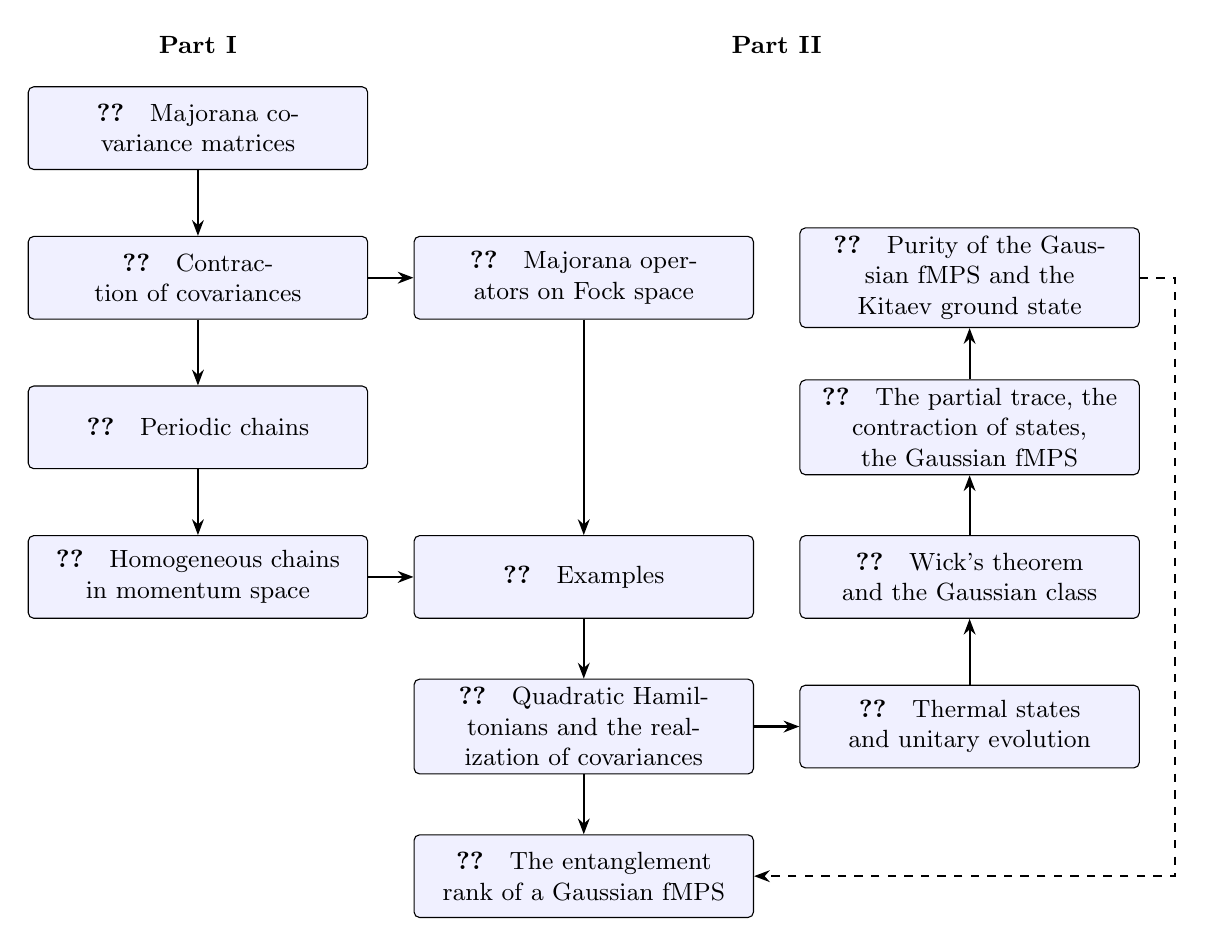
\begin{tikzpicture}[
  font=\small,
  done/.style={draw, rounded corners=2pt, fill=Blue!6, text width=4.1cm, align=center,
    minimum height=1.05cm, inner sep=3pt},
  dep/.style={-{Stealth[length=2mm]}, thick},
  ex/.style={dep, dashed}]
  \node[done] (s1) at (0,0) {\ref*{sec:majorana}\quad Majorana covariance matrices};
  \node[done] (s2) at (0,-1.9) {\ref*{sec:contraction}\quad Contraction of covariances};
  \node[done] (s3) at (0,-3.8) {\ref*{sec:chain}\quad Periodic chains};
  \node[done] (s4) at (0,-5.7) {\ref*{sec:fourier}\quad Homogeneous chains in momentum space};
  \node[done] (s5) at (4.9,-1.9) {\ref*{sec:fock}\quad Majorana operators on Fock space};
  \node[done] (s6) at (4.9,-5.7) {\ref*{sec:examples}\quad Examples};
  \node[done] (s7) at (4.9,-7.6) {\ref*{sec:hamiltonian}\quad Quadratic Hamiltonians and the realization of covariances};
  \node[done] (s12) at (4.9,-9.5) {\ref*{sec:entrank}\quad The entanglement rank of a Gaussian fMPS};
  \node[done] (s8) at (9.8,-7.6) {\ref*{sec:thermal}\quad Thermal states and unitary evolution};
  \node[done] (s9) at (9.8,-5.7) {\ref*{sec:wick}\quad Wick's theorem and the Gaussian class};
  \node[done] (s10) at (9.8,-3.8) {\ref*{sec:gaussianmap}\quad The partial trace, the contraction of states, the Gaussian fMPS};
  \node[done] (s11) at (9.8,-1.9) {\ref*{sec:fmps}\quad Purity of the Gaussian fMPS and the Kitaev ground state};
  \node[font=\small\bfseries] at (0,1.05) {Part I};
  \node[font=\small\bfseries] at (7.35,1.05) {Part II};
  \draw[dep] (s1) -- (s2);
  \draw[dep] (s2) -- (s3);
  \draw[dep] (s3) -- (s4);
  \draw[dep] (s2) -- (s5);
  \draw[dep] (s4) -- (s6);
  \draw[dep] (s5) -- (s6);
  \draw[dep] (s6) -- (s7);
  \draw[dep] (s7) -- (s8);
  \draw[dep] (s8) -- (s9);
  \draw[dep] (s9) -- (s10);
  \draw[dep] (s10) -- (s11);
  \draw[dep] (s7) -- (s12);
  \draw[ex] (s11.east) -- ++(0.45,0) |- (s12.east);
\end{tikzpicture}
\caption{\revs{Dependence of the sections. An arrow means that the later section uses the earlier
one, and arrows implied by chains of solid arrows are omitted; a chain records a possible
dependence through intermediate sections, not a use of every section on it. The dashed arrow is a
use in an example only: Corollary~\ref{cor:ent-rank} names the pure on-site covariances of
Corollary~\ref{cor:chain-pure} as one case of its hypothesis.}}
\label{fig:roadmap}
\end{figure}

\noindent\motiv{\revs{Several uses are narrower than the chains suggest. Sections~\ref{sec:hamiltonian}
to~\ref{sec:wick} use none of Sections~\ref{sec:contraction} to~\ref{sec:fourier}, and
Section~\ref{sec:hamiltonian} uses Section~\ref{sec:examples} only for Theorems~\ref{thm:gate}
and~\ref{thm:congruence}, which rest on Section~\ref{sec:fock} alone; Section~\ref{sec:fock} uses
Section~\ref{sec:contraction} only for Definition~\ref{def:bond}. Section~\ref{sec:gaussianmap}
uses Section~\ref{sec:chain} for the definitions of the chain and Lemma~\ref{lem:relabel}.
Theorem~\ref{thm:cross-rank} uses only Sections~\ref{sec:contraction} and~\ref{sec:chain};
Section~\ref{sec:entrank} uses Section~\ref{sec:hamiltonian} only for the normal form
(Theorem~\ref{thm:normal-form}) and Section~\ref{sec:examples} only in remarks \vet{and asides}.}}

\part{Covariance matrices}
\section{Majorana covariance matrices}
\label{sec:majorana}
For $n\geq0$, use coordinates $(x_1,\ldots,x_n,y_1,\ldots,y_n)$ on $\R^{2n}$; for
each mode $j$ we label its two Majorana operators $x_j$ and $y_j$. All matrices are
real unless stated otherwise, and $\|v\|^2=v^{\T}v$ is the squared Euclidean norm.
For a real symmetric matrix $A$, the notation $A\succeq0$ means $v^{\T}Av\geq0$ for
every real column vector $v$. For a complex matrix $H$, $H\succeq0$ means that
$H=H^*$ and $z^*Hz\geq0$ for every complex column vector $z$, where $H^*$ is the
conjugate transpose. We regard real matrices as complex matrices when they enter
the complex inequality. The case $n=0$ is included throughout: the empty matrix
satisfies every condition below.

\motiv{The two conditions of Definition~\ref{def:admissible} are the ones a state imposes. If
$c_1,\ldots,c_{2n}$ are Hermitian operators with $c_jc_k+c_kc_j=2\delta_{jk}$ and
$\rho$ is a density operator, the numbers $\Gamma_{jk}=\tfrac{\ii}{2}\tr(\rho[c_j,c_k])$
are real and antisymmetric, and $1+\ii\Gamma\succeq0$ is exactly the statement
$\tr(\rho A^*A)\geq0$ for the operators $A=\sum_j\overline{z_j}\,c_j$. Section~\ref{sec:fock}
proves both facts (Theorems~\ref{thm:reality} and~\ref{thm:admissible});
this section derives only what follows from the matrix conditions.}

\begin{definition}[Admissible covariance]\label{def:admissible}
A real $2n\times2n$ matrix $\Gamma$ is called \emph{admissible} (a physical covariance) if
\begin{equation}\label{eq:admissibility}
 \Gamma^{\T}=-\Gamma,\qquad 1-\Gamma^{\T}\Gamma\succeq0 .
\end{equation}
\end{definition}
The matrix $1-\Gamma^{\T}\Gamma$ is symmetric for every $\Gamma$, so the second
condition is the real positive semidefiniteness of a symmetric matrix.

\motiv{\revs{A second condition singles out the covariances of pure states: for a Gaussian state,
$\Gamma^2=-1$ holds exactly when the state is pure~\cite[Sec.~2]{bravyi}
(Theorem~\ref{thm:idempotent} in Section~\ref{sec:fmps}). Here the condition is taken as the
definition.}}

\begin{definition}[Pure covariance]\label{def:pure}
A real $2n\times2n$ matrix $\Gamma$ is called \emph{pure} if
$\Gamma^{\T}=-\Gamma$ and $\Gamma^2=-1$.
\end{definition}
\revs{A pure covariance is orthogonal, since $\Gamma^{\T}\Gamma=-\Gamma^2=1$, and it is a complex
structure on $\R^{2n}$: since $(\Gamma-\ii)(\Gamma+\ii)=\Gamma^2+1=0$, $\Gamma$ is diagonalizable
over $\C$ with eigenvalues $\pm\ii$ (a matrix annihilated by a polynomial with distinct roots is
diagonalizable), and complex conjugation maps the $\ii$-eigenspace onto the $-\ii$-eigenspace
because $\Gamma$ is real, so each has dimension $n$.}

For any real matrix $A$ and real vector $v$, $v^{\T}Av=v^{\T}A^{\T}v$; hence
$v^{\T}\Gamma v=0$ when $\Gamma$ is antisymmetric, and $a^{\T}\Gamma b=-b^{\T}\Gamma a$
for all real $a,b$. For any real matrix $O$ and real symmetric $A\succeq0$, the
congruence $OAO^{\T}$ is symmetric and
$v^{\T}OAO^{\T}v=(O^{\T}v)^{\T}A(O^{\T}v)\geq0$, so $OAO^{\T}\succeq0$.

\subsection{Equivalent forms of admissibility}

\begin{theorem}[Norm form]\label{thm:norm-form}
Let $\Gamma^{\T}=-\Gamma$. Then $\Gamma$ is admissible if and only if
$\|\Gamma v\|\leq\|v\|$ for every $v\in\R^{2n}$.
\end{theorem}
\begin{proof}
For real $v$, $v^{\T}(1-\Gamma^{\T}\Gamma)v=\|v\|^2-\|\Gamma v\|^2$.
\end{proof}

\motiv{The real form is the one the
operations of Section~\ref{subsec:operations} preserve
(Theorems~\ref{thm:orthogonal}--\ref{thm:sum}); the Hermitian form is the one a state
delivers, since $z^*(1+\ii\Gamma)z=\tr(\rho A^*A)$ for $A=\sum_j\overline{z_j}c_j$
(Theorem~\ref{thm:admissible}).}

\begin{theorem}[Hermitian form]\label{thm:hermitian-form}
Let $\Gamma^{\T}=-\Gamma$. Then $\Gamma$ is admissible if and only if
$1+\ii\Gamma\succeq0$ as a complex matrix.
\end{theorem}
\begin{proof}
The matrix $1+\ii\Gamma$ is Hermitian, since
$(\ii\Gamma)^*=-\ii\Gamma^{\T}=\ii\Gamma$. Write $z=a+\ii b$ with $a,b$ real.
Then $z^*=a^{\T}-\ii b^{\T}$ and
\[
 z^*(1+\ii\Gamma)z
 =(a^{\T}-\ii b^{\T})(a+\ii b)+\ii(a^{\T}-\ii b^{\T})\Gamma(a+\ii b)
 =\|a\|^2+\|b\|^2+\ii\bigl(\ii\,a^{\T}\Gamma b-\ii\,b^{\T}\Gamma a\bigr),
\]
using $a^{\T}\Gamma a=b^{\T}\Gamma b=0$. With $a^{\T}\Gamma b=-b^{\T}\Gamma a$ this gives
\begin{equation}\label{eq:hermitian-form}
 z^*(1+\ii\Gamma)z=\|a\|^2+\|b\|^2+2\,b^{\T}\Gamma a .
\end{equation}
Suppose $\|\Gamma a\|\leq\|a\|$ for all $a$. Expanding $0\leq\|b+\Gamma a\|^2$ gives
$2\,b^{\T}\Gamma a\geq-\|b\|^2-\|\Gamma a\|^2$, so the right side of
\eqref{eq:hermitian-form} is at least $\|a\|^2-\|\Gamma a\|^2\geq0$. Conversely, if
the right side is nonnegative for all $a,b$, the choice $b=-\Gamma a$ gives
$\|a\|^2-\|\Gamma a\|^2\geq0$. Theorem~\ref{thm:norm-form} completes both directions.
\end{proof}
\begin{remark}\label{rem:bosonic}
For bosonic covariances the corresponding condition is $\gamma-\ii\Omega_n\succeq0$
with $\Omega_n$ the symplectic form on the quadratures; for fermions the identity and
the symplectic form exchange roles. The coordinates $x_j,y_j$ of these notes label the
two Majorana operators of a mode and are not quadratures.
\end{remark}

\begin{theorem}[Purity]\label{thm:purity}
Every pure covariance is admissible, satisfies $\Gamma^{\T}\Gamma=1$, and is an
isometry: $\|\Gamma v\|=\|v\|$ for all $v$.
\end{theorem}
\begin{proof}
$\Gamma^{\T}\Gamma=-\Gamma^2=1$, so $1-\Gamma^{\T}\Gamma=0\succeq0$, and
$\|\Gamma v\|^2=v^{\T}\Gamma^{\T}\Gamma v=\|v\|^2$.
\end{proof}

\subsection{Changes of basis, subsystems and direct sums}
\label{subsec:operations}
\noindent A unitary $U$ that maps each Majorana operator to a real linear combination,
$Uc_jU^*=\sum_kO_{jk}c_k$ with $O$ real, has $O$ orthogonal, because the images again
satisfy $c_jc_k+c_kc_j=2\delta_{jk}$; the state $U^*\rho U$ then has covariance
$O\Gamma O^{\T}$~\cite[Sec.~2]{bravyi} ($U$ implements $O$ in the terminology of
Section~\ref{sec:hamiltonian}). Admissibility and purity survive this congruence
(Theorem~\ref{thm:orthogonal}). Discarding modes restricts $\Gamma$ to the remaining
coordinates; admissibility survives (Theorem~\ref{thm:subsystem}), purity need not
(Remark~\ref{rem:purity-subsystem}). Preparing two systems independently gives the direct
sum of their covariances, and admissibility and purity are decided blockwise
(Theorem~\ref{thm:sum}). We build matrix product states from these three operations
and a fourth, contraction (Section~\ref{sec:contraction}).

\begin{theorem}[Orthogonal congruence]\label{thm:orthogonal}
Let $O$ be a real $2n\times2n$ matrix with $OO^{\T}=1$. If $\Gamma$ is admissible,
then $O\Gamma O^{\T}$ is admissible; if $\Gamma$ is pure, then $O\Gamma O^{\T}$ is pure.
\end{theorem}
\begin{proof}
Since $O$ is square, $OO^{\T}=1$ makes $O$ invertible with inverse $O^{\T}$, so
$O^{\T}O=1$ as well. Antisymmetry:
$(O\Gamma O^{\T})^{\T}=O\Gamma^{\T}O^{\T}=-O\Gamma O^{\T}$. Inserting $O^{\T}O=1$,
$(O\Gamma O^{\T})^{\T}(O\Gamma O^{\T})=O\Gamma^{\T}\Gamma O^{\T}$, hence
$1-(O\Gamma O^{\T})^{\T}(O\Gamma O^{\T})=O(1-\Gamma^{\T}\Gamma)O^{\T}\succeq0$
by the congruence fact above. For purity,
$(O\Gamma O^{\T})^2=O\Gamma^2O^{\T}=-OO^{\T}=-1$.
\end{proof}

To select a subsystem, we take both Majorana coordinates of each chosen mode
together. An injective map $e:\{1,\ldots,m\}\to\{1,\ldots,n\}$ lists $m$ distinct
modes; write $\bar e(x_a)=x_{e(a)}$ and $\bar e(y_a)=y_{e(a)}$ for the induced map on
coordinates.

\begin{theorem}[Mode selection]\label{thm:subsystem}
Let $e$ be injective and let $\Gamma$ be admissible. Then the $2m\times2m$ matrix
$\Gamma'_{\alpha\beta}=\Gamma_{\bar e(\alpha)\bar e(\beta)}$ is admissible. The empty
selection $m=0$ is included.
\end{theorem}
\begin{proof}
Antisymmetry passes to the restriction, since
$\Gamma'_{\beta\alpha}=\Gamma_{\bar e(\beta)\bar e(\alpha)}=-\Gamma_{\bar e(\alpha)\bar e(\beta)}$.
For $v\in\R^{2m}$ let $\tilde v\in\R^{2n}$ have $\tilde v_{\bar e(\alpha)}=v_\alpha$ and
all other entries zero; this is well defined because $\bar e$ is injective, and
$\|\tilde v\|=\|v\|$. For each $\alpha$,
$(\Gamma'v)_\alpha=\sum_\beta\Gamma_{\bar e(\alpha)\bar e(\beta)}v_\beta=(\Gamma\tilde v)_{\bar e(\alpha)}$.
A sum of squares over the coordinates $\bar e(\alpha)$ is at most the sum over all
coordinates, so
$\|\Gamma'v\|^2\leq\|\Gamma\tilde v\|^2\leq\|\tilde v\|^2=\|v\|^2$ by
Theorem~\ref{thm:norm-form}, which then also gives admissibility of $\Gamma'$.
\end{proof}
\begin{remark}\label{rem:purity-subsystem}
Purity does not pass to subsystems: the reduced covariance of an entangled pure
state is not pure.
\end{remark}

For $\Gamma_1$ of size $2n_1$ and $\Gamma_2$ of size $2n_2$, the
\emph{direct sum} $\Gamma_1\oplus\Gamma_2$ (the covariance of two uncorrelated systems) is the $2(n_1+n_2)$ matrix with
entries $(\Gamma_1)$ on the coordinates of the first $n_1$ modes, $(\Gamma_2)$ on
those of the last $n_2$ modes, and zero cross entries, in the $(x,y)$ ordering of
the composite system.

\begin{theorem}[Independent sums]\label{thm:sum}
$\Gamma_1\oplus\Gamma_2$ is admissible if and only if $\Gamma_1$ and $\Gamma_2$ are
admissible, and pure if and only if both are pure.
\end{theorem}
\begin{proof}
Conjugation by the permutation matrix that groups the coordinates of each subsystem
together carries $\Gamma_1\oplus\Gamma_2$ to $\operatorname{diag}(\Gamma_1,\Gamma_2)$.
This conjugation is a ring isomorphism of matrices that commutes with
transposition and fixes $1$; it therefore carries antisymmetry,
$1-\Gamma^{\T}\Gamma$ and $\Gamma^2$ to the corresponding block-diagonal
quantities, and it preserves $\succeq0$ by the congruence fact with $O$ the
permutation matrix or its transpose. It remains to decide each property blockwise.
Transposition and products of block-diagonal matrices are blockwise, so
$\operatorname{diag}(\Gamma_1,\Gamma_2)$ is antisymmetric, or squares to $-1$,
exactly when both blocks do. For $v=(v_1,v_2)$,
\[
 v^{\T}\operatorname{diag}(A_1,A_2)v=v_1^{\T}A_1v_1+v_2^{\T}A_2v_2,
\]
so $\operatorname{diag}(A_1,A_2)\succeq0$ when both blocks are, and conversely
taking $v_2=0$ or $v_1=0$ isolates each block. Apply this with
$A_i=1-\Gamma_i^{\T}\Gamma_i$.
\end{proof}

\subsection{The standard covariance and one mode}
Let
\begin{equation}\label{eq:standard}
 \Omega_n=\begin{pmatrix}0&1_n\\-1_n&0\end{pmatrix}
\end{equation}
in the coordinates $(x,y)$. It is antisymmetric and $\Omega_n^2=-1$, so $\Omega_n$
is pure. On Fock
space, $\Omega_n$ is the covariance of the state with every mode occupied and $-\Omega_n$
that of the vacuum (Corollary~\ref{cor:vacuum}).
\motiv{The covariance of every state with a definite occupation in each mode is
$\Omega_n$ with the sign of each mode's $2\times2$ block chosen independently
(Theorem~\ref{thm:occupation}); Proposition~\ref{prop:one-mode} shows that these signed
blocks are the only pure one-mode covariances.}

\begin{proposition}[One mode]\label{prop:one-mode}
Every real antisymmetric $2\times2$ matrix has the form
$\Gamma_\lambda=\lambda\Omega_1$ with $\lambda\in\R$. $\Gamma_\lambda$ is admissible
if and only if $|\lambda|\leq1$, and pure if and only if $|\lambda|=1$.
\end{proposition}
\begin{proof}
Antisymmetry forces zero diagonal entries and opposite off-diagonal entries, which
is the stated form with $\lambda$ the $(x_1,y_1)$ entry. Then
$\Gamma_\lambda^{\T}\Gamma_\lambda=\lambda^2\cdot1$ and
$\Gamma_\lambda^2=-\lambda^2\cdot1$. For a real number $c$, the matrix $c\cdot1$
satisfies $c\cdot1\succeq0$ exactly when $c\geq0$, since $v^{\T}(c\cdot1)v=c\|v\|^2$;
with $c=1-\lambda^2$ this gives admissibility exactly when $\lambda^2\leq1$. Purity
is $-\lambda^2\cdot1=-1$, that is $\lambda^2=1$.
\end{proof}

\section{Contraction of covariances}
\label{sec:contraction}
\motiv{To build a matrix product state on a chain, we join the virtual indices of on-site
tensors by maximally entangled pairs and then sum over them. For Gaussian
states the on-site tensors are covariances, the pairs are the bond covariance of
Definition~\ref{def:bond}, and the summation is one operation on matrices, the
contraction of Definition~\ref{def:contract}: it eliminates the labels of the joined
modes and returns a covariance on the labels that remain. The result is
admissible whenever the inputs are (Theorem~\ref{thm:contract}), so that a chain built by
repeated contraction is a covariance at every stage, and contracting two bonds through a
bond returns a bond (Theorem~\ref{thm:teleport}), which fixes the sign of the bond.
That the contraction is the covariance of the state obtained by projecting the
eliminated modes onto the pair is the fermionic linear-optics
calculus~\cite[Sec.~4]{bravyi}, \cite[Sec.~II]{ksvc}; Section~\ref{sec:gaussianmap} proves it on
Fock space (Theorem~\ref{thm:state-contract}).}

In this section we call a real matrix $\Gamma$ indexed by an
arbitrary finite set $I$ \emph{admissible} if $\Gamma^{\T}=-\Gamma$ and
$1-\Gamma^{\T}\Gamma\succeq0$, and \emph{pure} if $\Gamma^{\T}=-\Gamma$ and
$\Gamma^2=-1$; on the Majorana labels of $n$ modes these are the conditions of
Section~\ref{sec:majorana}, and the norm form of Theorem~\ref{thm:norm-form} holds for
every finite $I$ with the same proof. ``$M$ invertible'' means $\det M\neq0$, and
$M^{-1}$ is then the inverse matrix. For disjoint index sets $I_1,I_2$, $I_1\sqcup I_2$
is their union, and we write a matrix on $I_1\sqcup I_2$ in blocks with the $I_1$
labels first. The \emph{direct sum} of $\Gamma_1$ on $I_1$ and $\Gamma_2$ on $I_2$
is $\operatorname{diag}(\Gamma_1,\Gamma_2)$ on $I_1\sqcup I_2$, the matrix
$\Gamma_1\oplus\Gamma_2$ of Theorem~\ref{thm:sum} after grouping each system's labels
together. A set of modes $L$ carries the Majorana labels $x_a,y_a$ for $a\in L$,
written $x_L,y_L$ collectively; $1_L$ is the identity matrix indexed by $L$.

\subsection{The contraction and its admissibility}
Let $I=R\sqcup E$ be split into \emph{retained} and \emph{eliminated} labels (in the chains of
Section~\ref{sec:chain}: the physical and the virtual Majorana labels), and write
a matrix on $I$ in blocks
\[
 \Gamma=\begin{pmatrix}A&B\\C&D\end{pmatrix},\qquad
 A\in\R^{R\times R},\ B\in\R^{R\times E},\ C\in\R^{E\times R},\ D\in\R^{E\times E}.
\]
Let $\Gamma_p$ be a matrix on $E$, the \emph{pair covariance}.

\begin{definition}[Contraction]\label{def:contract}
If $1-D\Gamma_p$ is invertible,
\[
 \Gamma\star\Gamma_p=A+B\,\Gamma_p\,(1-D\Gamma_p)^{-1}C ,
\]
a matrix on $R$.
\end{definition}
\motiv{The formula is the Schur complement of the eliminated block of a $2\times2$
block system: if $(x,w)\mapsto(u,v)$ is the linear map $\Gamma$ and we impose $w=\Gamma_pv$
on the eliminated coordinates, then $u=(\Gamma\star\Gamma_p)x$
(displayed in the proof of Theorem~\ref{thm:contract}). The contraction preserves
admissibility because $\Gamma$ and $\Gamma_p$ are norm-nonincreasing (Theorem~\ref{thm:norm-form}),
hence so is $x\mapsto u$. For a pure $\Gamma_p$ the formula becomes
$A+B\,(D+\Gamma_p)^{-1}B^{\T}$ (Theorem~\ref{thm:pure-bond}), the form
of~\cite[Sec.~II]{ksvc}; the sign agrees with that reference once the pair is oriented as
in Definition~\ref{def:bond}, with $+1$ from the first copy to the second, and reversing the
orientation replaces $\Gamma_p$ by $-\Gamma_p$.}

\begin{lemma}[Push-through]\label{lem:push}
For square $X,Y$ of the same size, $\det(1-XY)=\det(1-YX)$, and if $1-XY$ is invertible
then $Y(1-XY)^{-1}=(1-YX)^{-1}Y$.
\end{lemma}
\begin{proof}
The determinant identity is Sylvester's: both sides equal the determinant of the block
matrix $\begin{pmatrix}1&X\\Y&1\end{pmatrix}$, obtained by eliminating either diagonal
block. From $Y(1-XY)=Y-YXY=(1-YX)Y$, multiply by $(1-YX)^{-1}$ on the left and
$(1-XY)^{-1}$ on the right.
\end{proof}

\begin{theorem}[Antisymmetry]\label{thm:antisym}
Let $\Gamma^{\T}=-\Gamma$, $\Gamma_p^{\T}=-\Gamma_p$, and $1-D\Gamma_p$ invertible. Then
$(\Gamma\star\Gamma_p)^{\T}=-\Gamma\star\Gamma_p$.
\end{theorem}
\begin{proof}
Antisymmetry of $\Gamma$ gives $A^{\T}=-A$, $D^{\T}=-D$ and $C=-B^{\T}$, so
$C^{\T}=-B$; antisymmetry of $\Gamma_p$ and $D$ gives
$(1-D\Gamma_p)^{\T}=1-\Gamma_p^{\T}D^{\T}=1-\Gamma_pD$. Then
\begin{align*}
 \bigl(B\Gamma_p(1-D\Gamma_p)^{-1}C\bigr)^{\T}
 &=C^{\T}\bigl((1-D\Gamma_p)^{\T}\bigr)^{-1}\Gamma_p^{\T}B^{\T}
 =(-B)(1-\Gamma_pD)^{-1}(-\Gamma_p)B^{\T}\\
 &=B\,(1-\Gamma_pD)^{-1}\Gamma_p\,B^{\T}
 =B\,\Gamma_p(1-D\Gamma_p)^{-1}B^{\T}
 =-B\,\Gamma_p(1-D\Gamma_p)^{-1}C ,
\end{align*}
using Lemma~\ref{lem:push} with $X=D$, $Y=\Gamma_p$ in the second line and then
$B^{\T}=-C$. So the second term changes sign under transposition, as does $A$.
\end{proof}

\begin{theorem}[Admissibility of the contraction]\label{thm:contract}
Let $\Gamma$ and $\Gamma_p$ be admissible and $1-D\Gamma_p$ invertible. Then
$\Gamma\star\Gamma_p$ is admissible.
\end{theorem}
\begin{proof}
Antisymmetry is Theorem~\ref{thm:antisym}; by the norm form it remains to show
$\|(\Gamma\star\Gamma_p)x\|\leq\|x\|$ for real $x\in\R^R$.
\begin{enumerate}
\item[(a)] Put
\[
 v=(1-D\Gamma_p)^{-1}Cx\in\R^E,\qquad w=\Gamma_pv\in\R^E,\qquad u=Ax+Bw\in\R^R .
\]
Then $u=(\Gamma\star\Gamma_p)x$ by definition, and $(1-D\Gamma_p)v=Cx$ gives
$v=Cx+Dw$. Hence
\[
 \Gamma\begin{pmatrix}x\\w\end{pmatrix}
 =\begin{pmatrix}Ax+Bw\\Cx+Dw\end{pmatrix}=\begin{pmatrix}u\\v\end{pmatrix}.
\]
\item[(b)] Admissibility of $\Gamma$ in norm form gives
$\|u\|^2+\|v\|^2\leq\|x\|^2+\|w\|^2$, and admissibility of $\Gamma_p$ gives
$\|w\|^2=\|\Gamma_pv\|^2\leq\|v\|^2$. Adding, $\|u\|^2\leq\|x\|^2$.
\end{enumerate}
\end{proof}
\begin{remark}\label{rem:invertibility}
Admissibility of $\Gamma$ and $\Gamma_p$ does not imply that $1-D\Gamma_p$ is
invertible: for $\Gamma=\begin{pmatrix}0&0\\0&D\end{pmatrix}$ with $D$ pure and
$\Gamma_p=-D$, $1-D\Gamma_p=1-1=0$. \motiv{For a pure pair covariance, Theorem~\ref{thm:pure-bond} turns the hypothesis into the
invertibility of $D+\Gamma_p$, which we check directly in each example.}
\end{remark}

\begin{theorem}[Pure pair covariances]\label{thm:pure-bond}
Let $\Gamma^{\T}=-\Gamma$ and let $\Gamma_p$ be pure. Then $1-D\Gamma_p$ is invertible
if and only if $D+\Gamma_p$ is, and in that case
\[
 \Gamma\star\Gamma_p=A+B\,(D+\Gamma_p)^{-1}B^{\T} .
\]
\end{theorem}
\begin{proof}
\begin{enumerate}
\item[(a)] Since $\Gamma_p^2=-1$, $\Gamma_p(-\Gamma_p)=1$, so $-\Gamma_p$ is invertible
with $(-\Gamma_p)^{-1}=\Gamma_p$, and
$(D+\Gamma_p)(-\Gamma_p)=-D\Gamma_p+1=1-D\Gamma_p$. Taking determinants, $\det(1-D\Gamma_p)$
and $\det(D+\Gamma_p)$ vanish together.
\item[(b)] When they do not vanish,
$(1-D\Gamma_p)^{-1}=(-\Gamma_p)^{-1}(D+\Gamma_p)^{-1}=\Gamma_p(D+\Gamma_p)^{-1}$, hence
$\Gamma_p(1-D\Gamma_p)^{-1}=\Gamma_p^2(D+\Gamma_p)^{-1}=-(D+\Gamma_p)^{-1}$ and, with
$C=-B^{\T}$, $B\Gamma_p(1-D\Gamma_p)^{-1}C=B(D+\Gamma_p)^{-1}B^{\T}$.
\end{enumerate}
\end{proof}
For a pair covariance that is not pure the two expressions differ \revs{in general}.

\subsection{The bond covariance and teleportation}
Let $L$ and $L'$ be two sets of modes matched by a bijection $a\mapsto a'$, with
Majorana labels $(x_L,x_{L'},y_L,y_{L'})$. In the chain of Section~\ref{sec:chain} the
first copy $L$ is the left virtual set of a site and the second copy $L'$ the right
virtual set of the previous site; we orient the bond from the first copy to the second,
$\beta_{x_ax_{a'}}=+1$.

\begin{definition}[Bond covariance]\label{def:bond}
The bond covariance on $L\sqcup L'$ is
\[
 \beta=\begin{pmatrix}J&0\\0&-J\end{pmatrix},\qquad
 J=\begin{pmatrix}0&1_L\\-1_L&0\end{pmatrix},
\]
where the outer blocks are the $x$ and $y$ labels and the inner blocks of $J$ are
$L$ and $L'$: $\beta_{x_ax_{a'}}=+1$, $\beta_{y_ay_{a'}}=-1$, all other entries zero.
\end{definition}
\motiv{For one pair of modes, $\beta$ has $\ii c_{x_a}c_{x_{a'}}$ and
$-\ii c_{y_a}c_{y_{a'}}$ both of expectation $1$; in the vacuum of
Corollary~\ref{cor:vacuum} the nonzero expectations are instead $\ii c_{x_a}c_{y_a}$
within one mode. The two-mode state with covariance $\beta$ is Theorem~\ref{thm:bondstate}.}

\begin{theorem}[Purity of the bond]\label{thm:bond-pure}
$\beta$ is pure.
\end{theorem}
\begin{proof}
$J^{\T}=-J$ and $J^2=-1$, so $\beta^{\T}=-\beta$ and
$\beta^2=\operatorname{diag}(J^2,J^2)=-1$.
\end{proof}

\begin{figure}[t]
\centering
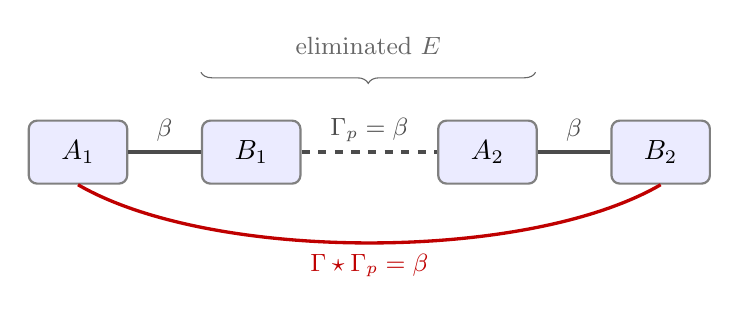
\begin{tikzpicture}[
  blk/.style={draw=black!50,fill=blue!8,thick,rounded corners=3pt,minimum width=1.25cm,minimum height=0.8cm},
  bond/.style={very thick,black!70},
  elim/.style={very thick,black!70,dashed},
  res/.style={very thick,red!75!black},
  lab/.style={font=\small}]
  \node[blk] (A1) at (0,0) {$A_1$};
  \node[blk] (B1) at (2.2,0) {$B_1$};
  \node[blk] (A2) at (5.2,0) {$A_2$};
  \node[blk] (B2) at (7.4,0) {$B_2$};
  \draw[bond] (A1) -- node[above,lab] {$\beta$} (B1);
  \draw[elim] (B1) -- node[above,lab] {$\Gamma_p=\beta$} (A2);
  \draw[bond] (A2) -- node[above,lab] {$\beta$} (B2);
  \draw[res] (A1.south) .. controls (1.7,-1.4) and (5.7,-1.4) .. node[below,lab] {$\Gamma\star\Gamma_p=\beta$} (B2.south);
  \draw[decorate,decoration={brace,amplitude=4pt,mirror},black!60] (B1.north west) ++(0,0.6) -- node[above=3pt,lab] {eliminated $E$} ++(4.25,0);
\end{tikzpicture}
\caption{Teleportation (Theorem~\ref{thm:teleport}). Each block is a copy of the
virtual label set $L$; solid lines are the bonds $\beta$ on $(A_1,B_1)$ and $(A_2,B_2)$,
the dashed line is the pair covariance $\Gamma_p=\beta$ on the eliminated labels
$E=B_1\sqcup A_2$. Contracting returns the bond $\beta$ on the retained pair $(A_1,B_2)$,
with the same sign and the same $x,y$ roles.}
\label{fig:teleport}
\end{figure}
\begin{theorem}[Teleportation]\label{thm:teleport}
Let two systems $I_1=A_1\sqcup B_1$ and $I_2=A_2\sqcup B_2$, each a matched pair of
copies of $L$, carry the bond covariance $\beta$ on $(A_1,B_1)$ and on $(A_2,B_2)$, and
let $\Gamma$ be their direct sum on $I_1\sqcup I_2$. Retain $R=A_1\sqcup B_2$,
eliminate $E=B_1\sqcup A_2$, and take $\Gamma_p=\beta$ on $(B_1,A_2)$. Then
$1-D\Gamma_p$ is invertible and $\Gamma\star\Gamma_p=\beta$ on $(A_1,B_2)$.
\end{theorem}
\begin{proof}
Neither bond has an entry within $A_1\sqcup B_2$ or within $B_1\sqcup A_2$, so $A=0$
and $D=0$; hence $1-D\Gamma_p=1$ is invertible and
$\Gamma\star\Gamma_p=B\Gamma_pC=-B\Gamma_pB^{\T}$. All matrices are block diagonal in the
$x$ and $y$ labels. In the $x$ sector the two bonds contribute $J$ on $(A_1,B_1)$ and on
$(A_2,B_2)$, so the retained--eliminated block is
\[
 B=\begin{array}{c|cc}
    & x_{B_1} & x_{A_2}\\ \hline
  x_{A_1} & 1_L & 0\\
  x_{B_2} & 0 & -1_L
 \end{array}
\]
and $\Gamma_p=J$ on $(B_1,A_2)$. Then
\[
 -BJB^{\T}
 =-\begin{pmatrix}1_L&0\\0&-1_L\end{pmatrix}\begin{pmatrix}0&1_L\\-1_L&0\end{pmatrix}\begin{pmatrix}1_L&0\\0&-1_L\end{pmatrix}
 =-\begin{pmatrix}0&-1_L\\1_L&0\end{pmatrix}=J
\]
on $(x_{A_1},x_{B_2})$. In the $y$ sector $B$ and $\Gamma_p$ both change sign, so
$-B\Gamma_pB^{\T}$ changes sign and equals $-J$ on $(y_{A_1},y_{B_2})$. Together,
$\Gamma\star\Gamma_p=\beta$ on $(A_1,B_2)$.
\end{proof}
Theorem~\ref{thm:teleport} (Figure~\ref{fig:teleport}) fixes the convention: with the bond of
Definition~\ref{def:bond} used both as the on-site resource and as the contracted pair,
contraction reproduces the bond without a change of sign or of the $x,y$ roles. Here
we orient the contracted pair from $B_1$ to $A_2$. The chain of Section~\ref{sec:chain}
orients its inter-site pairs the other way, from $A_{i+1}$ to $B_i$; since $A=0$ and $D=0$
here, the contraction is linear in $\Gamma_p$, and with the chain orientation the same
computation returns $-\beta$ on $(A_1,B_2)$, that is $\beta$ on $(B_2,A_1)$.

\section{Periodic chains}
\label{sec:chain}
\motiv{\rev{A Gaussian fermionic matrix product state on a ring of $N$ sites has, at each
site, $P$ physical modes and two sets of $M$ virtual modes; neighbouring sites share a
maximally entangled pair of virtual sets, and projecting every pair gives the state of the
physical modes (Figure~\ref{fig:ring}). On covariances this is one contraction
against the bond covariance $\beta$ (Definition~\ref{def:periodic}).}
The result is admissible whenever the on-site covariances are, since the bond is pure
(Theorem~\ref{thm:periodic}); we compute a three-site example in closed form
(Proposition~\ref{prop:three}).}

\revs{The sites of the ring are $i\in\mathbb Z/N$, identified with $\{0,\ldots,N-1\}$ (the empty
set for $N=0$), with successor $i+1$ read modulo $N$, and the numbers $N,M,P\geq0$ are arbitrary. As in Figure~\ref{fig:ring}, site $i$ carries $M$ left virtual modes
$A_i$, $M$ right virtual modes $B_i$ and $P$ physical modes $C_i$, with the Majorana labels
$I_{\mathrm{site}}=(x_A,x_B,x_C,y_A,y_B,y_C)$; a family of labels indexed by (site, site label) is
ordered \emph{site by site} when all labels of site $0$ come first, then those of site $1$, and so
on. The pairs (site, mode) form the sets $Q=\{(i,c):i\in\mathbb Z/N,\ c\in\{1,\ldots,P\}\}$ for the
physical modes and $L=\{(i,a):i\in\mathbb Z/N,\ a\in\{1,\ldots,M\}\}$ for the virtual ones; the bond
of Definition~\ref{def:bond} will be placed on $L\sqcup L'$ with $L'$ a second copy of $L$, and
$x^{L}_{(i,a)}$, $x^{L'}_{(i,a)}$ denote the $x$-labels of the two copies.}

\subsection{\rev{The covariance of a periodic chain}}
\revs{Collecting the labels of all sites into the split $R\sqcup E$ of
Section~\ref{sec:contraction} reorders them, and one notation records the reordering. For an index
bijection $e:I\to I'$ and a matrix $\Gamma$ on $I'$, the relabelled matrix $\Gamma^e$ on $I$ has
entries $(\Gamma^e)_{ab}=\Gamma_{e(a)e(b)}$.}
\begin{definition}[\rev{On-site covariances and the input matrix}]\label{def:input}
\rev{The on-site covariances are matrices $\Gamma_i$ on $I_{\mathrm{site}}$, one per site.} The input
matrix is obtained by stacking them block-diagonally, site by site, and then permuting
rows and columns so that the physical labels come first and the virtual labels follow,
grouped as the pairs $(A_i,B_{i-1})$ that the bonds join. In symbols, let
$R=(x_Q,y_Q)$ and $E=(x_L,x_{L'},y_L,y_{L'})$, and define $e:R\sqcup E\to\bigsqcup_iI_i$ by
\[
 e(x_{(i,c)})=x_{C_i,c},\quad e(x_{(i,a)}^{L})=x_{A_i,a},\quad e(x_{(i,a)}^{L'})=x_{B_{i-1},a},
\]
and the same with $y$ in place of $x$; $e$ is a bijection. The \emph{\rev{input matrix}}
is $\Gamma_{\mathrm{in}}=\bigl(\operatorname{diag}(\Gamma_i)_{i}\bigr)^{e}$, a matrix
on $R\sqcup E$.
\end{definition}
$\operatorname{diag}(\Gamma_i)$ is the direct sum over sites, ordered site by site; the
shift $i-1$ in the $L'$ labels makes $(A_i,B_{i-1})$ the matched pair $(L,L')$ of
Definition~\ref{def:bond}, $L$ the left virtual set of site $i$ and $L'$ the right
virtual set of site $i-1$.

\begin{definition}[\rev{Bonds of the chain and its covariance}]\label{def:periodic}
\rev{The bonds of the chain form the matrix} $\beta_N=\beta$ on $E$, the bond covariance of $L\sqcup L'$:
$(\beta_N)_{x_{A_i,a}\,x_{B_{i-1},a}}=1$, $(\beta_N)_{y_{A_i,a}\,y_{B_{i-1},a}}=-1$, all
other entries zero. If $1-D\beta_N$ is invertible, where $D$ is the $E\times E$ block of
$\Gamma_{\mathrm{in}}$, the \emph{\rev{covariance of the chain}} \rev{with on-site covariances $\Gamma_\bullet$} is
\[
 \Gamma_N(\Gamma_\bullet)=\Gamma_{\mathrm{in}}\star\beta_N ,
\]
a matrix on $R$.
\end{definition}

\begin{figure}[t]
\centering
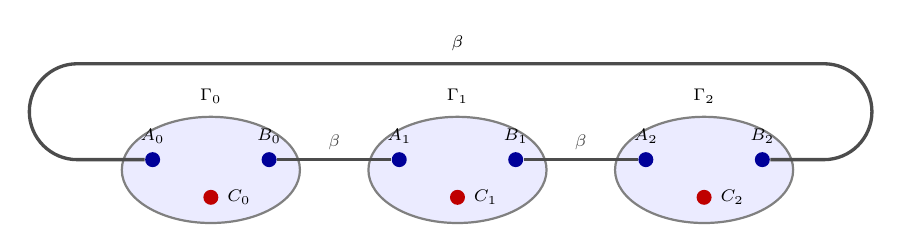
\begin{tikzpicture}[scale=0.87,transform shape,
  blob/.style={draw=black!50,fill=blue!8,thick,ellipse,minimum width=2.6cm,minimum height=1.55cm},
  virt/.style={circle,fill=blue!60!black,inner sep=2.2pt},
  phys/.style={circle,fill=red!75!black,inner sep=2.2pt},
  pair/.style={very thick,black!70},
  lab/.style={font=\scriptsize}]
  \foreach \i/\x in {0/0,1/3.6,2/7.2} {
    \node[blob] (G\i) at (\x,0) {};
    \node[lab,anchor=south] at (\x,0.85) {$\Gamma_{\i}$};
    \node[virt] (A\i) at (\x-0.85,0.15) {};
    \node[virt] (B\i) at (\x+0.85,0.15) {};
    \node[phys] (C\i) at (\x,-0.4) {};
    \node[lab,anchor=south] at (A\i.north) {$A_{\i}$};
    \node[lab,anchor=south] at (B\i.north) {$B_{\i}$};
    \node[lab,anchor=west] at (C\i.east) {$C_{\i}$};
  }
  \draw[pair] (B0) -- node[above,lab] {$\beta$} (A1);
  \draw[pair] (B1) -- node[above,lab] {$\beta$} (A2);
  \draw[pair] (B2) -- ++(0.9,0) arc (-90:90:0.7) -- ++(-10.9,0) arc (90:270:0.7) -- (A0);
  \node[lab] at (3.6,1.85) {$\beta$};
\end{tikzpicture}
\caption{The periodic chain for $N=3$, $M=P=1$, drawn as in \cite[Fig.~1]{ksvc}. Dots are
modes: the virtual modes $A_i,B_i$ (blue) and the physical mode $C_i$ (red). A line joining
$B_i$ to $A_{i+1}$ is the maximally entangled pair of Theorem~\ref{thm:bondstate}, whose
covariance is $\beta$ on the ordered pair $(L,L')=(A_{i+1},B_i)$, $\beta_{x_{A_{i+1}}x_{B_i}}=1$.
The shaded region around site $i$ is the on-site covariance $\Gamma_i$ on $A_i,B_i,C_i$;
projecting every pair leaves a state of the physical modes, and on covariances this is the
contraction of Definition~\ref{def:periodic}.}
\label{fig:ring}
\end{figure}

\begin{lemma}[Relabelling and direct sums]\label{lem:relabel}
Let $e:I\to I'$ be a bijection. $\Gamma$ on $I'$ is admissible (pure) if and only if
$\Gamma^e$ is. If $\Gamma_i$ are matrices on $I_i$, then $\operatorname{diag}(\Gamma_i)_i$ on
$\bigsqcup_iI_i$ is admissible if and only if every $\Gamma_i$ is.
\end{lemma}
\begin{proof}
\begin{enumerate}
\item[(a)] $(\Gamma^e)^{\T}=(\Gamma^{\T})^e$, $\Gamma^e\Delta^e=(\Gamma\Delta)^e$,
$1^e=1$, and $(\Gamma^ev)\cdot(\Gamma^ev)=(\Gamma\tilde v)\cdot(\Gamma\tilde v)$,
$v\cdot v=\tilde v\cdot\tilde v$ for $\tilde v=v\circ e^{-1}$. Antisymmetry and
$\Gamma^2=-1$ transfer by the first three identities; the norm form of
Theorem~\ref{thm:norm-form} transfers by the last two.
\item[(b)] Transposition of a block-diagonal matrix is blockwise, and
$(\operatorname{diag}(\Gamma_i)v)\cdot(\operatorname{diag}(\Gamma_i)v)=\sum_i(\Gamma_iv_i)\cdot(\Gamma_iv_i)$,
$v\cdot v=\sum_iv_i\cdot v_i$ with $v_i$ the restriction of $v$ to $I_i$. The norm
inequality for $\operatorname{diag}(\Gamma_i)$ follows from those of the blocks by
summing; conversely $v$ supported on one block isolates that block.
\end{enumerate}
\end{proof}

\begin{theorem}[\rev{The chain covariance is admissible}]\label{thm:periodic}
Let every $\Gamma_i$ be admissible and $1-D\beta_N$ invertible. Then
$\Gamma_N(\Gamma_\bullet)$ is admissible.
\end{theorem}
\begin{proof}
$\beta_N$ is pure (Theorem~\ref{thm:bond-pure}), hence admissible.
$\Gamma_{\mathrm{in}}$ is admissible by Lemma~\ref{lem:relabel}. Apply
Theorem~\ref{thm:contract}.
\end{proof}
\begin{remark}\label{rem:small-chains}
\revf{For $N=1$ the bond joins $B_0$ to $A_0$ within the site.}
\end{remark}


\subsection{\rev{Three sites}}
Take $N=3$ and $M=P=1$. Then $I_{\mathrm{site}}=(x_A,x_B,x_C,y_A,y_B,y_C)$, $R$ consists of the six
labels $x_{C_0},x_{C_1},x_{C_2},y_{C_0},y_{C_1},y_{C_2}$, and $E$ of the twelve labels
$x^{L}_i,\ x^{L'}_i,\ y^{L}_i,\ y^{L'}_i$ ($i\in\mathbb Z/3$, in this order of groups),
with $x^{L}_i=x_{A_i}$ and $x^{L'}_i=x_{B_{i-1}}$. Let $\Gamma_{\mathrm{seed}}$ be the direct sum of the
bond covariance $\beta$ on $(A,B)$ (Definition~\ref{def:bond}) and $-\Omega_1$ on $C$, that is
$(\Gamma_{\mathrm{seed}})_{x_Cy_C}=-1$ (Corollary~\ref{cor:vacuum}), and let $O$ be the rotation with
$O_{x_Ax_A}=O_{y_Cy_C}=\tfrac35$, $O_{x_Ay_C}=-\tfrac45$, $O_{y_Cx_A}=\tfrac45$ and
$O=1$ on the other four labels. The on-site covariance at every site is
\[
 \Gamma_{\mathrm{site}}=O\,\Gamma_{\mathrm{seed}}\,O^{\T}=\frac15\begin{pmatrix}
 0&3&-4&0&0&0\\ -3&0&0&0&0&-4\\ 4&0&0&0&0&-3\\ 0&0&0&0&-5&0\\ 0&0&0&5&0&0\\ 0&4&3&0&0&0
 \end{pmatrix},
\]
pure by Theorem~\ref{thm:orthogonal}.

\begin{proposition}[Three-site chain]\label{prop:three}
\rev{For the on-site covariances} $\Gamma_i=\Gamma_{\mathrm{site}}$, $i\in\mathbb Z/3$:
$\det(1-D\beta_3)=(304/125)^2\neq0$, and in the labels $(x_{C_0},x_{C_1},x_{C_2},y_{C_0},y_{C_1},y_{C_2})$
\[
 \Gamma_3(\Gamma_\bullet)=\begin{pmatrix}0&-\Theta\\\Theta^{\T}&0\end{pmatrix},\qquad
 \Theta=\frac1{19}\begin{pmatrix}15&-6&10\\10&15&-6\\-6&10&15\end{pmatrix},
\]
which is pure ($\Theta\Theta^{\T}=1$) and translation invariant ($\Theta$ is circulant).
\end{proposition}
\begin{proof}
\begin{enumerate}
\item[(a)] The blocks of $\Gamma_{\mathrm{in}}$: $A=-\tfrac35\Omega_3$, with $\Omega_3$ as in~\eqref{eq:standard}, from the
$(x_C,y_C)$ entry of $\Gamma_{\mathrm{site}}$ at each site; $B$ has the entries
$B_{x_{C_i}x^{L}_i}=\tfrac45$ and $B_{y_{C_i}x^{L'}_{i+1}}=\tfrac45$ (the entries
$(x_C,x_A)$ and $(y_C,x_B)$ of $\Gamma_{\mathrm{site}}$; the label $x_{B_i}$ is
$x^{L'}_{i+1}$) and no others; $C=-B^{\T}$; $D$ is the $(x_A,x_B,y_A,y_B)$ block of
$\Gamma_{\mathrm{site}}$ at each site, relabelled by $e$. \revs{Let $\mathsf S$ be the cyclic shift on $\mathbb Z/3$,
$\mathsf S_{i,i+1}=1$, so that $\mathsf S^{\T}=\mathsf S^{-1}=\mathsf S^2$. With the eliminated labels in the groups
$(x^L,x^{L'},y^L,y^{L'})$ and the retained labels in the groups $(x_C,y_C)$,}
\[\revs{
 B=\tfrac45\begin{pmatrix}1&0&0&0\\0&\mathsf S&0&0\end{pmatrix},\qquad
 D=\begin{pmatrix}0&\tfrac35\mathsf S&0&0\\-\tfrac35\mathsf S^{\T}&0&0&0\\0&0&0&-\mathsf S\\0&0&\mathsf S^{\T}&0\end{pmatrix},\qquad
 \beta_3=\begin{pmatrix}0&1&0&0\\-1&0&0&0\\0&0&0&-1\\0&0&1&0\end{pmatrix}.}
\]
\item[(b)] $D$ couples $x^{L}_i=x_{A_i}$ to $x^{L'}_{i+1}=x_{B_i}$ and $\beta_3$ couples
$x^{L'}_{i+1}$ back to $x^{L}_{i+1}$, and likewise for $y$, so $D\beta_3$ maps each of the
four label groups $x^{L},x^{L'},y^{L},y^{L'}$ to itself by a circulant matrix. Hence
$1-D\beta_3$ and its inverse $Y$ are block diagonal in these four groups with circulant
blocks, and $\det(1-D\beta_3)=(304/125)^2$. \revs{Explicitly,
$1-D\beta_3=\operatorname{diag}\bigl(1+\tfrac35\mathsf S,\,1+\tfrac35\mathsf S^{\T},\,1+\mathsf S,\,1+\mathsf S^{\T}\bigr)$. Since
$\mathsf S^3=1$ and the eigenvalues of $\mathsf S$ are the cube roots of unity,
$\det(1+\tfrac35\mathsf S)=1+(\tfrac35)^3=\tfrac{152}{125}$ and $\det(1+\mathsf S)=2$, the same for
$\mathsf S^{\T}$, and $(1+\tfrac35\mathsf S)^{-1}=\tfrac{125}{152}(1-\tfrac35\mathsf S+\tfrac9{25}\mathsf S^2)$,
$(1+\mathsf S)^{-1}=\tfrac12(1-\mathsf S+\mathsf S^2)$. Hence
$\det(1-D\beta_3)=(152/125)^2\cdot2^2$ and}
\[\revs{
 152\,Y=\operatorname{diag}\bigl(125-75\mathsf S+45\mathsf S^2,\ 125-75\mathsf S^{\T}+45\mathsf S,\ 76(1-\mathsf S+\mathsf S^2),\
 76(1-\mathsf S^{\T}+\mathsf S)\bigr).}
\]
\item[(c)] $\Gamma_3=A+B\beta_3YC$ is the stated matrix. The blocks of $152Y$ are integer circulant
matrices, and we evaluate the products blockwise. \revs{Only the $x^L$ and $x^{L'}$ blocks
$Y_L=(1+\tfrac35\mathsf S)^{-1}$ and $Y_{L'}=(1+\tfrac35\mathsf S^{\T})^{-1}$ of $Y$ enter, and}
\[\revs{
 B\beta_3YC=-\tfrac{16}{25}\begin{pmatrix}0&Y_{L'}\mathsf S^{\T}\\-\mathsf SY_L&0\end{pmatrix}
 =\frac1{95}\begin{pmatrix}0&-(18-30\mathsf S+50\mathsf S^{\T})\\(18-30\mathsf S+50\mathsf S^{\T})^{\T}&0\end{pmatrix}.}
\]
\revs{Adding $A=-\tfrac35\Omega_3$ gives $\Theta=\tfrac35+\tfrac1{95}(18-30\mathsf S+50\mathsf S^{\T})=\tfrac1{19}(15-6\mathsf S+10\mathsf S^{\T})$, the
stated circulant matrix, and $\Theta\Theta^{\T}=\tfrac1{361}\bigl(361+60(\mathsf S+\mathsf S^{\T})-60(\mathsf S^2+(\mathsf S^{\T})^2)\bigr)=1$
since $\mathsf S^2=\mathsf S^{\T}$.}

{\sloppy\artefact{\revs{In the formalization},
$5\Gamma_{\mathrm{site}}$, $152Y$ and $19\Theta$ are integer matrices; the identities
$(1-D\beta_3)(152Y)=152\cdot1$ and $72200\,(A+B\beta_3YC)=72200\,\Gamma_3$ are decided
over $\mathbb Z$ by evaluation and then divided.}\par}
\end{enumerate}
\end{proof}
The physical modes are correlated: $\Gamma_{x_{C_i}y_{C_{i+1}}}=6/19$ and
$\Gamma_{x_{C_i}y_{C_{i-1}}}=-10/19$.
\motiv{For pure on-site covariances $\Gamma_N$ is pure (Corollary~\ref{cor:chain-pure}; \revs{like
Corollary~\ref{cor:cov-pure}, a fact about the matrices of Part~I whose proof in these notes goes
through Fock space}), and
Section~\ref{sec:gaussianmap} constructs the state of the physical modes whose
covariance is $\Gamma_N$.}

\paragraph{Checks.} {\small\sloppy\revs{Every quantity in the proof of Proposition~\ref{prop:three}, the
determinant included, is recomputed in exact rational arithmetic by
\path{checks/three_site_exact.py}, which also prints the full matrices $1-D\beta_3$, $Y$ and
$B\beta_3YC$.}}

\section{Homogeneous chains in momentum space}
\label{sec:fourier}
\motiv{When every site of the periodic chain of Section~\ref{sec:chain} carries the same
on-site covariance $\Gamma$, the chain covariance commutes with the shift of sites, and
the discrete Fourier transform over sites splits it into $N$ blocks of size $2P\times2P$,
one per momentum $k$. Each block is again a contraction (Definition~\ref{def:contract}),
now of a single site against a single bond, with the shift of the right virtual modes
turned into a phase, and the inverse transform recovers $\Gamma_N$ from its blocks;
antisymmetry and admissibility of $\Gamma$ pass to every block.}

Throughout this section $N\geq1$ and $M,P\geq0$; the on-site covariances are
$\Gamma_i=\Gamma$ for every site, a fixed real matrix on $I_{\mathrm{site}}=(x_A,x_B,x_C,y_A,y_B,y_C)$, and
$\Gamma_N=\Gamma_N(\Gamma,\ldots,\Gamma)$ is the covariance of the chain
(Definition~\ref{def:periodic}), with $D$ the $E\times E$ block of $\Gamma_{\mathrm{in}}$.
We write retained labels as $(i,a)$ with $i\in\mathbb Z/N$ the site and
$a\in R_0=(x_C,y_C)$ one of the $2P$ physical labels of a site. The site labels split as
$I_{\mathrm{site}}=R_0\sqcup E_0$ with $E_0=(x_A,x_B,y_A,y_B)$; $\beta_M$ is the real bond covariance of
$E_0$ (Definition~\ref{def:bond} with $L=A$, $L'=B$ and the index set $\{1,\ldots,M\}$).
For a complex matrix $X$, $X^*$ is the conjugate transpose, $\overline X$ the entrywise
conjugate, and $X^{-1}$ the inverse of an invertible $X$.

\subsection{Twisted on-site covariances}
\begin{definition}[Characters and the twisted on-site covariance]\label{def:twist}
For $k,i\in\mathbb Z/N$ let $\chi_k(i)=e^{-2\pi\ii\,ki/N}$ and $\omega_k=\chi_k(1)$.
The \emph{twist} $t_k:I_{\mathrm{site}}\to\C$ is $t_k(u)=\omega_k$ for $u\in\{x_B,y_B\}$ and
$t_k(u)=1$ otherwise, and the \emph{twisted on-site covariance} at momentum $k$ (the on-site covariance conjugated by
the momentum phase on the right virtual modes) is
\[
 \Gamma^{(k)}=\operatorname{diag}(t_k)\,\Gamma\,\operatorname{diag}(t_k)^*,\qquad
 \Gamma^{(k)}_{uv}=t_k(u)\,\Gamma_{uv}\,\overline{t_k(v)} .
\]
\end{definition}
With this sign of $\chi_k$, Theorem~\ref{thm:reconstruct} expands $\Gamma_N$ in
$e^{+2\pi\ii\,k(i-j)/N}\,\Sigma(k)$. \vet{The opposite convention expands in} $e^{-2\pi\ii\,k(i-j)/N}$, and
in that convention the block at momentum $k$ is $\Sigma(-k)=\overline{\Sigma(k)}$
(Theorem~\ref{thm:blocks}(a)).

\begin{definition}[Momentum-space covariance]\label{def:symbol}
Write $\Gamma^{(k)}=\begin{pmatrix}A_k&B_k\\C_k&D_k\end{pmatrix}$ in the split
$I_{\mathrm{site}}=R_0\sqcup E_0$. The \emph{momentum-space covariance} at $k$ (the symbol of the
block-circulant matrix $\Gamma_N$) is the complex $R_0\times R_0$ matrix
\[
 \Sigma(k)=A_k+B_k\,\beta_M\,(1-D_k\beta_M)^{-1}\,C_k ,
\]
the contraction formula of Definition~\ref{def:contract} applied over $\C$ to $\Gamma^{(k)}$
and the bond of one site.
\end{definition}
\artefact{When $1-D_k\beta_M$ is singular, we read $\Sigma(k)$ with $(1-D_k\beta_M)^{-1}=0$,
the value of the formalization's inverse on singular matrices; only
Theorem~\ref{thm:blocks}(a) uses $\Sigma(k)$ in that case.}

\begin{definition}[Fourier coefficients of the chain]\label{def:fourier}
For $k,l\in\mathbb Z/N$ and $a,b\in R_0$,
\[
 \widehat{\Gamma}_N(k,l)_{ab}=\frac1N\sum_{i,j\in\mathbb Z/N}\chi_k(i)\,(\Gamma_N)_{(i,a)(j,b)}\,\overline{\chi_l(j)} .
\]
\end{definition}

\subsection{The Fourier transform of the chain}
Let $\Phi_N$ be the $N\times N$ matrix with entries $(\Phi_N)_{ki}=\chi_k(i)/\sqrt N$; by the
orthogonality of characters, $\sum_i\chi_k(i)\overline{\chi_l(i)}=N\delta_{kl}$, it is
unitary. Identify the retained labels with pairs, $R\cong(\mathbb Z/N)\times R_0$ by
$(i,a)$, and the eliminated labels likewise, $E\cong(\mathbb Z/N)\times E_0$ by
$x^{L}_{(i,a)}\mapsto(i,x_{A,a})$, $x^{L'}_{(i,a)}\mapsto(i,x_{B,a})$ and the same for $y$;
a label $(i,u)$ with $u\in\{x_B,y_B\}$ is thus the right virtual mode of site $i-1$
(Definition~\ref{def:input}). Let $\Phi_R=\Phi_N\otimes1_{R_0}$,
$\Phi_E=\Phi_N\otimes1_{E_0}$ and $\Phi=\Phi_R\oplus\Phi_E$ on $R\sqcup E$.

\begin{lemma}[Block diagonalization of the input]\label{lem:input-blocks}
$\Phi_E\beta_N\Phi_E^*=\beta_N$, and $\Phi\Gamma_{\mathrm{in}}\Phi^*=\bigoplus_{k}\Gamma^{(k)}$ in the
split $R\sqcup E$, that is, the four blocks of $\Phi\Gamma_{\mathrm{in}}\Phi^*$ are
$\bigoplus_kA_k$, $\bigoplus_kB_k$, $\bigoplus_kC_k$, $\bigoplus_kD_k$.
\end{lemma}
\begin{proof}
\begin{enumerate}
\item[(a)] In the pair identification, $\beta_N=1_N\otimes\beta_M$, because the bond
pairs $x^{L}_{(i,a)}$ with $x^{L'}_{(i,a)}$ at the same pair $(i,a)$
(Definition~\ref{def:periodic}); it commutes with $\Phi_N\otimes1$.
\item[(b)] Let $s(u)=1$ for $u\in\{x_B,y_B\}$ and $s(u)=0$ otherwise. The label $(i,u)$
with $u\in\{x_B,y_B\}$ names a mode of site $i-1$, and $\operatorname{diag}(\Gamma_\bullet)$
is site diagonal, so
$(\Gamma_{\mathrm{in}})_{(i,u)(j,v)}=\Gamma_{uv}\,[\,i-s(u)=j-s(v)\,]$. Hence
\[
 (\Phi\Gamma_{\mathrm{in}}\Phi^*)_{(k,u)(l,v)}
 =\frac{\Gamma_{uv}}N\sum_{i}\chi_k(i)\,\overline{\chi_l(i-s(u)+s(v))}
 =\delta_{kl}\,\Gamma_{uv}\,\omega_k^{\,s(u)}\,\overline{\omega_k}^{\,s(v)}
 =\delta_{kl}\,\Gamma^{(k)}_{uv},
\]
by $\chi_l(i+m)=\chi_l(i)\chi_l(m)$, $\chi_l(1)=\omega_l$, and orthogonality; the last
equality is Definition~\ref{def:twist}. \qedhere
\end{enumerate}
\end{proof}

\begin{lemma}[Contraction and relabelling]\label{lem:contract-conj}
Let $\Gamma$ be a matrix on $R\sqcup E$, $\Gamma_p$ a matrix on $E$ with $1-D\Gamma_p$
invertible, and $Y_R$, $Y_E$ invertible matrices on the retained and on the eliminated
labels. Then, with the contraction formula taken over $\C$,
\[
 \begin{pmatrix}Y_RAY_R^{-1}&Y_RBY_E^{-1}\\Y_ECY_R^{-1}&Y_EDY_E^{-1}\end{pmatrix}\star(Y_E\Gamma_pY_E^{-1})
 =Y_R\,(\Gamma\star\Gamma_p)\,Y_R^{-1} .
\]
If $\Gamma=\bigoplus_k\Gamma_k$ and $\Gamma_p=\bigoplus_k\Gamma_{p,k}$ are block diagonal
in a common index $k$, then $\det(1-D\Gamma_p)=\prod_k\det(1-D_k\Gamma_{p,k})$, and when
this is nonzero, $\Gamma\star\Gamma_p=\bigoplus_k\Gamma_k\star\Gamma_{p,k}$.
\end{lemma}
\begin{proof}
$1-Y_EDY_E^{-1}\,Y_E\Gamma_pY_E^{-1}=Y_E(1-D\Gamma_p)Y_E^{-1}$, whose inverse is
$Y_E(1-D\Gamma_p)^{-1}Y_E^{-1}$; the four products then telescope. For block
diagonal data, determinants multiply over blocks, the inverse of an invertible block
diagonal matrix is block diagonal with the inverse blocks, and sums and products are
blockwise.
\end{proof}

\begin{theorem}[Determinant factorization]\label{thm:det-factor}
$\det(1-D\beta_N)=\prod_{k\in\mathbb Z/N}\det(1-D_k\beta_M)$. In particular, if
$1-D\beta_N$ is invertible then $1-D_k\beta_M$ is invertible for every $k$.
\end{theorem}
\begin{proof}
$\Phi_E(1-D\beta_N)\Phi_E^*=1-\bigoplus_kD_k\beta_M$ by Lemma~\ref{lem:input-blocks};
$\Phi_E$ is unitary, so the determinants agree, and the block determinant is the product
(Lemma~\ref{lem:contract-conj}). A nonzero product has nonzero factors.
\end{proof}

\begin{theorem}[Translation invariance and diagonalization]\label{thm:diagonal}
Let $1-D\beta_N$ be invertible. Then for all $i,j\in\mathbb Z/N$, $k,l\in\mathbb Z/N$
and $a,b\in R_0$,
\[
 (\Gamma_N)_{(i+1,a)(j+1,b)}=(\Gamma_N)_{(i,a)(j,b)},
 \qquad
 \widehat{\Gamma}_N(k,l)=\begin{cases}\Sigma(k)&k=l,\\0&k\neq l.\end{cases}
\]
\end{theorem}
\begin{theorem}[Reconstruction]\label{thm:reconstruct}
Let $1-D\beta_N$ be invertible. Then for all $i,j\in\mathbb Z/N$ and $a,b\in R_0$,
\[
 (\Gamma_N)_{(i,a)(j,b)}=\frac1N\sum_{k\in\mathbb Z/N}\overline{\chi_k(i)}\,\Sigma(k)_{ab}\,\chi_k(j).
\]
\end{theorem}
\begin{proof}[Proof of Theorems~\ref{thm:diagonal} and~\ref{thm:reconstruct}]
\begin{enumerate}
\item[(a)] By Lemma~\ref{lem:input-blocks}, Lemma~\ref{lem:contract-conj} with
$Y=\Phi$ (so $Y^{-1}=\Phi^*$), and Theorem~\ref{thm:det-factor},
\[
 \Phi_R\,\Gamma_N\,\Phi_R^*=(\Phi\Gamma_{\mathrm{in}}\Phi^*)\star(\Phi_E\beta_N\Phi_E^*)
 =\Bigl(\bigoplus_k\Gamma^{(k)}\Bigr)\star\Bigl(\bigoplus_k\beta_M\Bigr)=\bigoplus_k\Sigma(k).
\]
\item[(b)] The $((k,a),(l,b))$ entry of the left side is $\widehat{\Gamma}_N(k,l)_{ab}$
by the definition of $\Phi_R$; this is the second part of Theorem~\ref{thm:diagonal}.
\item[(c)] Multiplying (a) by $\Phi_R^*$ on the left and $\Phi_R$ on the right gives
$\Gamma_N=\Phi_R^*\bigl(\bigoplus_k\Sigma(k)\bigr)\Phi_R$, whose $((i,a),(j,b))$ entry is the
sum of Theorem~\ref{thm:reconstruct}.
\item[(d)] $\overline{\chi_k(i+1)}\,\chi_k(j+1)=\overline{\chi_k(i)}\,\overline{\omega_k}\,\chi_k(j)\,\omega_k=\overline{\chi_k(i)}\,\chi_k(j)$,
so replacing $(i,j)$ by $(i+1,j+1)$ leaves the sum in (c) unchanged; this is the first
part of Theorem~\ref{thm:diagonal}. \qedhere
\end{enumerate}
\end{proof}
\begin{remark}\label{rem:singular}
The invertibility hypothesis enters translation invariance only through this route; the
chain construction is shift symmetric, and we make no claim here about the singular case.
\end{remark}

\subsection{Admissibility in momentum space}
\begin{theorem}[Symmetries and admissibility of the momentum-space covariance]\label{thm:blocks}
\begin{enumerate}
\item[(a)] If $1-D_k\beta_M$ is invertible then $\Sigma(-k)=\overline{\Sigma(k)}$;
\artefact{the \revs{formalized} statement holds for every $k$, with the inverse of a singular matrix read as $0$.}
\item[(b)] If $\Gamma^{\T}=-\Gamma$ and $1-D\beta_N$ is invertible, then
$\Sigma(k)^*=-\Sigma(k)$ for every $k$.
\item[(c)] If $\Gamma$ is admissible (Definition~\ref{def:admissible}) and $1-D\beta_N$
is invertible, then $1-\Sigma(k)^*\Sigma(k)\succeq0$ for every $k$, that is,
$\|\Sigma(k)z\|\leq\|z\|$ for every $z\in\C^{R_0}$.
\end{enumerate}
\end{theorem}
\begin{proof}
\begin{enumerate}
\item[(a)] $\omega_{-k}=\overline{\omega_k}$, so $t_{-k}=\overline{t_k}$ and, $\Gamma$
being real, $\revs{\Gamma^{(-k)}}=\overline{\Gamma^{(k)}}$; $\beta_M$ is real, and the inverse, read as
$0$ on singular matrices, commutes with entrywise conjugation, so
the formula of Definition~\ref{def:symbol} commutes with conjugation.
\item[(b)] $\Gamma_N^{\T}=-\Gamma_N$ (Theorem~\ref{thm:antisym}, applied to
$\Gamma_{\mathrm{in}}$, which is antisymmetric with $\Gamma$, and to $\beta_N$), and
$\Gamma_N$ is real, so $\Gamma_N^*=-\Gamma_N$ and $\Phi_R\Gamma_N\Phi_R^*$ is skew-Hermitian;
by step (a) of the proof of Theorem~\ref{thm:diagonal} its blocks $\Sigma(k)$ are skew-Hermitian.
\item[(c)] $\Gamma_N$ is admissible (Theorem~\ref{thm:periodic}), so
$1-\Gamma_N^{\T}\Gamma_N\succeq0$ over $\R$, hence over $\C$: for $z=a+\ii b$ with $a,b$
real, $z^*Xz=a^{\T}Xa+b^{\T}Xb$ when $X$ is real symmetric. Conjugating by $\Phi_R$ and
using step (a) of the proof of Theorem~\ref{thm:diagonal},
$\Phi_R(1-\Gamma_N^{\T}\Gamma_N)\Phi_R^*=1-\bigoplus_k\Sigma(k)^*\Sigma(k)\succeq0$, and a
block diagonal matrix is positive semidefinite exactly when each block is (test with
vectors supported on one block). \qedhere
\end{enumerate}
\end{proof}
\motiv{Part (c) is the momentum-space form of admissibility. For pure $\Gamma$ the chain
covariance $\Gamma_N$ is pure (Corollary~\ref{cor:chain-pure}, a matrix fact whose proof in these notes
goes through Fock space), and the argument of (c) with
$1-\Gamma_N^{\T}\Gamma_N=0$ gives $\Sigma(k)^*\Sigma(k)=1$ for every $k$.}

\part{States on Fock space}
\section{Majorana operators on Fock space}
\label{sec:fock}
A \emph{configuration} of $n$ modes is a map $s:\{1,\ldots,n\}\to\{0,1\}$; $s_j$ is
the occupation of mode $j$. Fock space is $\mathcal F_n=\C^{\{0,1\}^n}$ with the standard basis
$\{|s\rangle\}$, and operators on it are complex matrices indexed by configurations.
For a matrix $M$, $M^*$ is its conjugate transpose, and $1$ denotes the identity of
whatever size the context requires. For a configuration $s$ let $s^{(j)}$ be $s$
with the occupation of mode $j$ replaced by $s_j+1$ modulo $2$; then
$(s^{(j)})^{(j)}=s$ and $(s^{(j)})^{(k)}=(s^{(k)})^{(j)}$. Write $\varsigma(b)=(-1)^b$
for $b\in\{0,1\}$, so $\varsigma(s_j+1)=-\varsigma(s_j)$, and $[\,\cdot\,]$ for the number $1$ if
the statement in the bracket holds and $0$ otherwise.

\begin{definition}[Pauli matrices and the string]\label{def:pauli}
For each mode $j$ define
\[
 (X_j)_{st}=[t=s^{(j)}],\qquad
 Z_j=\operatorname{diag}\bigl(\varsigma(s_j)\bigr)_s,\qquad
 Z_{<j}=\operatorname{diag}\Bigl(\prod_{k<j}\varsigma(s_k)\Bigr)_s .
\]
\end{definition}
$X_j$ is the permutation matrix of the flip of mode $j$; $Z_j$ and $Z_{<j}$ are real
diagonal, and $Z_{<1}=1$.
\motiv{The matrices $X_j$ and $X_k$ of
different modes commute (Lemma~\ref{lem:pauli}(b)), and so do the diagonal matrices
$Z_j$ and $Z_k$; operators built from these alone would commute across modes, whereas
Theorem~\ref{thm:car} requires $c_\alpha c_\beta=-c_\beta c_\alpha$ for labels of
different modes. $Z_{<j}$ records the parity of the modes before $j$, and
Lemma~\ref{lem:pauli}(e) says that $X_j$ reverses that parity exactly when $j$ lies
before the string's mode; this is the sign rule Theorem~\ref{thm:car} uses. The
ordering of modes is a convention; a different ordering gives operators related to
these by a unitary conjugation, which we do not prove here.}

\begin{lemma}[Commutation rules]\label{lem:pauli}
For all modes $j,k$:
\begin{enumerate}
\item[(a)] $X_j^2=Z_j^2=Z_{<j}^2=1$, and $X_j,Z_j,Z_{<j}$ are real symmetric.
\item[(b)] $(X_jX_k)_{st}=[t=(s^{(j)})^{(k)}]$; hence $X_jX_k=X_kX_j$, and
 $(X_jX_k)_{ss}=[j=k]$.
\item[(c)] For a diagonal matrix $D=\operatorname{diag}(d_s)$,
 $X_jD=D'X_j$ with $D'=\operatorname{diag}(d_{s^{(j)}})$.
\item[(d)] $X_jZ_j=-Z_jX_j$, and $X_jZ_k=Z_kX_j$ for $k\neq j$.
\item[(e)] $X_jZ_{<k}=\eta_{jk}Z_{<k}X_j$, where $\eta_{jk}=-1$ if $j<k$ and
 $\eta_{jk}=1$ otherwise.
\end{enumerate}
\end{lemma}
\begin{proof}
\begin{enumerate}
\item[(a)] $(X_j^2)_{st}=\sum_u[u=s^{(j)}][t=u^{(j)}]=[t=s]$; $Z_j^2$ and $Z_{<j}^2$ are
diagonal with entries $\varsigma(\cdot)^2=1$. Symmetry of $X_j$: $t=s^{(j)}$ if and only
if $s=t^{(j)}$.
\item[(b)] $(X_jX_k)_{st}=\sum_u[u=s^{(j)}][t=u^{(k)}]=[t=(s^{(j)})^{(k)}]$. The two
flips commute, and $(s^{(j)})^{(k)}=s$ exactly when $j=k$, since for $j\neq k$ the
configuration $(s^{(j)})^{(k)}$ differs from $s$ at mode $j$.
\item[(c)] $(X_jD)_{st}=\sum_u[u=s^{(j)}]\,d_u[u=t]=d_{s^{(j)}}[t=s^{(j)}]=(D'X_j)_{st}$.
\item[(d)] By (c) with $d_s=\varsigma(s_j)$, $d_{s^{(j)}}=-\varsigma(s_j)$; for $k\neq j$,
$d_s=\varsigma(s_k)$ is unchanged by flipping mode $j$.
\item[(e)] By (c) with $d_s=\prod_{k'<k}\varsigma(s_{k'})$: flipping mode $j$ changes the
sign of the factor $k'=j$ if $j<k$ and of no factor otherwise.
\end{enumerate}
\end{proof}

\begin{definition}[Majorana operators]\label{def:majorana}
With Majorana labels $x_1,\ldots,x_n,y_1,\ldots,y_n$ as in Section~\ref{sec:majorana},
the Jordan--Wigner operators are
\[
 c_{x_j}=Z_{<j}X_j,\qquad c_{y_j}=\ii\,Z_{<j}X_jZ_j .
\]
\end{definition}
$X_j$, $Z_j$ and $\ii X_jZ_j=\sigma^y_j$ are the Pauli matrices $\sigma^x_j,\sigma^z_j,\sigma^y_j$
of mode $j$, so $c_{x_j}=Z_{<j}\sigma^x_j$ and $c_{y_j}=Z_{<j}\sigma^y_j$ with $Z_{<j}$ the
Jordan--Wigner string.
For one mode, in the basis $(|0\rangle,|1\rangle)$,
\[
 c_{x_1}=X_1=\begin{pmatrix}0&1\\1&0\end{pmatrix},\qquad
 c_{y_1}=\ii X_1Z_1=\begin{pmatrix}0&-\ii\\ \ii&0\end{pmatrix}.
\] The annihilation operator of mode $j$ is
$a_j=\tfrac12(c_{x_j}+\ii c_{y_j})=\tfrac12Z_{<j}X_j(1-Z_j)$; since $Z_{<j}$ and $X_j$ commute
(Lemma~\ref{lem:pauli}(e)),
\[
 a_j^*a_j=\tfrac14(1-Z_j)X_jZ_{<j}Z_{<j}X_j(1-Z_j)=\tfrac14(1-Z_j)^2=\tfrac12(1-Z_j)
 =\operatorname{diag}(s_j)_s ,
\]
the number operator of mode $j$, and
$\ii\,c_{x_j}c_{y_j}=\ii\cdot\ii\,Z_{<j}X_jZ_{<j}X_jZ_j=-Z_j=2a_j^*a_j-1$. For one mode
$a_1=|0\rangle\langle1|$, and $c_{x_1}=a_1+a_1^*$, $c_{y_1}=\ii(a_1^*-a_1)$.

Every Majorana operator is a \emph{signed flip}, a permutation matrix of one bit flip with signs on the entries. By Lemma~\ref{lem:pauli}(c),
\begin{equation}\label{eq:signed-flip}
 c_{x_j}=\operatorname{diag}(f_{x_j})\,X_j,\qquad c_{y_j}=\operatorname{diag}(f_{y_j})\,X_j,
 \qquad
 f_{x_j}(s)=\prod_{k<j}\varsigma(s_k),\quad
 f_{y_j}(s)=-\ii\,\varsigma(s_j)\prod_{k<j}\varsigma(s_k),
\end{equation}
where for $c_{y_j}$ we move the factor $Z_j=\operatorname{diag}(\varsigma(s_j))$ through
$X_j$, which turns it into $\operatorname{diag}(\varsigma(s_j+1))=\operatorname{diag}(-\varsigma(s_j))$.
For labels $\alpha,\beta$ with modes
$j,k$, Lemma~\ref{lem:pauli}(c) gives the product formula
\begin{equation}\label{eq:product}
 c_\alpha c_\beta=\operatorname{diag}\bigl(f_\alpha(s)\,f_\beta(s^{(j)})\bigr)\,X_jX_k .
\end{equation}

Within one mode, $\sigma^x_j$ and $\sigma^y_j$ are Pauli matrices: they square to $1$ and
anticommute. For $j<k$ the string $Z_{<k}$ contains the factor $Z_j$, which anticommutes with
the $X_j$ in $c_{x_j}$ and $c_{y_j}$, while every other factor of one operator commutes with
every factor of the other; the string supplies the sign between different modes.

\begin{theorem}[Canonical anticommutation relations]\label{thm:car}
For all Majorana labels $\alpha,\beta$,
\[
 c_\alpha c_\beta+c_\beta c_\alpha=2\delta_{\alpha\beta}\,1,\qquad c_\alpha^*=c_\alpha .
\]
\end{theorem}
\begin{proof}
By \eqref{eq:product} and Lemma~\ref{lem:pauli}(b), the anticommutator equals
$\operatorname{diag}(g_{\alpha\beta})\,X_jX_k$ with
\[
 g_{\alpha\beta}(s)=f_\alpha(s)f_\beta(s^{(j)})+f_\beta(s)f_\alpha(s^{(k)}) .
\]
Flipping mode $j$ multiplies $\prod_{k'<k}\varsigma(s_{k'})$ by $\eta_{jk}$ and
$\varsigma(s_j)$ by $-1$; for $j\neq k$, $\eta_{jk}+\eta_{kj}=0$. Write
$p_j=\prod_{k'<j}\varsigma(s_{k'})$ and $\sigma_j=\varsigma(s_j)$. Then $g_{\alpha\beta}(s)$ is:
\begin{enumerate}
\item[(i)] $j\neq k$, $\alpha=x_j$, $\beta=x_k$: $p_jp_k(\eta_{jk}+\eta_{kj})=0$.
\item[(ii)] $j\neq k$, $\alpha=x_j$, $\beta=y_k$: $-\ii\,p_jp_k\sigma_k(\eta_{jk}+\eta_{kj})=0$;
 the case $\alpha=y_j$, $\beta=x_k$ is the same with $\sigma_j$.
\item[(iii)] $j\neq k$, $\alpha=y_j$, $\beta=y_k$: $(-\ii)^2p_jp_k\sigma_j\sigma_k(\eta_{jk}+\eta_{kj})=0$.
\item[(iv)] $j=k$, $\{\alpha,\beta\}=\{x_j,y_j\}$: $-\ii\,p_j^2\bigl(\varsigma(s_j+1)+\sigma_j\bigr)=0$.
\item[(v)] $\alpha=\beta=x_j$: $2p_j^2=2$; $\alpha=\beta=y_j$:
 $2(-\ii)^2p_j^2\sigma_j\varsigma(s_j+1)=2$.
\end{enumerate}
For $\alpha\neq\beta$ the anticommutator is therefore $0$; for $\alpha=\beta$ it is
$\operatorname{diag}(2)\,X_j^2=2\cdot1$ by (a).

Hermiticity: by (a) and (c),
$c_\alpha^*=X_j\operatorname{diag}(\overline{f_\alpha})
=\operatorname{diag}\bigl(\overline{f_\alpha(s^{(j)})}\bigr)X_j$, and
$\overline{f_\alpha(s^{(j)})}=f_\alpha(s)$: for $x_j$ the product $p_j$ does not involve
mode $j$; for $y_j$,
$\overline{-\ii\,\varsigma(s_j+1)p_j}=\ii\,(-\sigma_j)p_j=f_{y_j}(s)$.
\end{proof}

\subsection{Covariance of a density operator}
\motiv{The covariance collects the second moments $\tr(\rho\,c_\alpha c_\beta)$; by
Theorem~\ref{thm:car} their symmetric part is fixed, $\tr(\rho\,c_\alpha c_\beta)+\tr(\rho\,c_\beta c_\alpha)=2\delta_{\alpha\beta}$,
so only the antisymmetric part carries information about $\rho$, and the factor
$\tfrac{\ii}{2}$ makes it real. A state is Gaussian when Wick's rule (Definition~\ref{def:wick})
determines all its higher moments from these; in closed form,
$\tr(\rho\,c_{\alpha_1}\cdots c_{\alpha_{2k}})$ is then the Pfaffian
of the $2k\times2k$ submatrix of $-\ii\Gamma$ on the \vet{distinct} labels $\alpha_1,\ldots,\alpha_{2k}$,
and odd moments vanish~\cite[Sec.~2]{bravyi}.}

\begin{definition}[Density operator and covariance]\label{def:density}
A \emph{density operator} is a matrix $\rho$ on $\mathcal F_n$ with $\rho\succeq0$ and
$\tr\rho=1$. Its \emph{Majorana covariance} is the real $2n\times2n$ matrix
\begin{equation}\label{eq:covariance}
 \Gamma(\rho)_{\alpha\beta}=\Re\Bigl(\tfrac{\ii}{2}\tr\bigl(\rho\,[c_\alpha,c_\beta]\bigr)\Bigr),
 \qquad [c_\alpha,c_\beta]=c_\alpha c_\beta-c_\beta c_\alpha .
\end{equation}
\end{definition}
A density operator is a \emph{pure state} when $\rho=|\psi\rangle\langle\psi|$ for a unit
vector $\psi$; equivalently $\rho^2=\rho$, since a positive
semidefinite matrix with $\rho^2=\rho$ and $\tr\rho=1$ has eigenvalues in $\{0,1\}$ summing
to $1$.

\begin{theorem}[Reality and antisymmetry]\label{thm:reality}
Let $\rho=\rho^*$. Then $\tfrac{\ii}{2}\tr(\rho[c_\alpha,c_\beta])$ is real, and
$\Gamma(\rho)^{\T}=-\Gamma(\rho)$, $\Gamma(\rho)_{\alpha\alpha}=0$, and
$\Gamma(\rho)_{\alpha\beta}=\Re\bigl(\ii\tr(\rho\,c_\alpha c_\beta)\bigr)$ for $\alpha\neq\beta$.
\end{theorem}
\begin{proof}
Put $T=\tr(\rho[c_\alpha,c_\beta])$. Since $\tr(M^*)=\overline{\tr M}$ and
$[c_\alpha,c_\beta]^*=c_\beta c_\alpha-c_\alpha c_\beta$ by Theorem~\ref{thm:car},
$\overline T=\tr\bigl([c_\alpha,c_\beta]^*\rho\bigr)=-\tr\bigl([c_\alpha,c_\beta]\rho\bigr)=-T$
using $\tr(AB)=\tr(BA)$. Hence $T$ is purely imaginary and $\tfrac{\ii}{2}T$ is real.
Antisymmetry is $[c_\beta,c_\alpha]=-[c_\alpha,c_\beta]$; the diagonal vanishes since
$[c_\alpha,c_\alpha]=0$; for $\alpha\neq\beta$, Theorem~\ref{thm:car} gives
$[c_\alpha,c_\beta]=2c_\alpha c_\beta$. The last three statements hold for every $\rho$.
\end{proof}

\motiv{Restricted to a single mode, the inequality of Theorem~\ref{thm:admissible} reads as follows.
With $z$ supported on the labels $x_j,y_j$ and $z_{x_j}=\tfrac12$,
$z_{y_j}=-\tfrac{\ii}{2}$, the operator $A=\sum_\alpha\overline{z_\alpha}c_\alpha$ is
$a_j=\tfrac12(c_{x_j}+\ii c_{y_j})$ and
$z^*(1+\ii\Gamma)z=\tfrac12\bigl(1+\Gamma_{x_jy_j}\bigr)=\tr(\rho\,a_j^*a_j)$, the occupation
of mode $j$. Theorem~\ref{thm:admissible}
is this positivity for every $A=\sum_\alpha\overline{z_\alpha}c_\alpha$ at once, and
Theorem~\ref{thm:occupation} shows that the bound is attained.}

\begin{theorem}[Admissibility]\label{thm:admissible}
For every density operator $\rho$, the covariance $\Gamma(\rho)$ is admissible.
\end{theorem}
\begin{proof}
Write $\Gamma=\Gamma(\rho)$; it is antisymmetric by Theorem~\ref{thm:reality}, so by
Theorem~\ref{thm:hermitian-form} it suffices to show $1+\ii\Gamma\succeq0$. Fix
$z\in\C^{2n}$ and put $A=\sum_\alpha\overline{z_\alpha}\,c_\alpha$, so
$A^*=\sum_\alpha z_\alpha c_\alpha$. Theorem~\ref{thm:car} gives
$c_\alpha c_\beta=\delta_{\alpha\beta}\,1+\tfrac12[c_\alpha,c_\beta]$, hence
\[
 A^*A=\sum_{\alpha,\beta}z_\alpha\overline{z_\beta}\,c_\alpha c_\beta
 =\|z\|^2\,1+\tfrac12\sum_{\alpha,\beta}z_\alpha\overline{z_\beta}\,[c_\alpha,c_\beta] .
\]
Taking the trace against $\rho$, with $\tr\rho=1$ and
$\tfrac12\tr(\rho[c_\alpha,c_\beta])=-\ii\,\Gamma_{\alpha\beta}$ by
\eqref{eq:covariance} and Theorem~\ref{thm:reality},
\[
 \tr(\rho A^*A)=\|z\|^2-\ii\sum_{\alpha,\beta}\overline{z_\beta}\,\Gamma_{\alpha\beta}\,z_\alpha
 =\|z\|^2-\ii\,z^*\Gamma^{\T}z=\|z\|^2+\ii\,z^*\Gamma z=z^*(1+\ii\Gamma)z .
\]
Finally $\tr(\rho A^*A)=\tr(A\rho A^*)\geq0$: for every vector $w$,
$w^*(A\rho A^*)w=(A^*w)^*\rho\,(A^*w)\geq0$, so $A\rho A^*\succeq0$, and a positive
semidefinite matrix has nonnegative diagonal entries, hence nonnegative trace.
\end{proof}
\revf{Conversely, every admissible matrix is the covariance of some density operator
(Theorem~\ref{thm:realization}).}

\subsection{Occupation-number states}
For a configuration $s$ let $\rho_s=|s\rangle\langle s|$, the matrix with a single
entry $1$ at position $(s,s)$. It is a pure state, and $\tr(\rho_sM)=M_{ss}$; for $s\equiv0$
it is the vacuum $\rho_{\mathrm{vac}}$.
\motiv{These are product states: each mode is definitely empty or definitely
occupied, and Theorem~\ref{thm:occupation} shows that the covariance is a direct sum of
the one-mode blocks $\pm\Omega_1$ of Proposition~\ref{prop:one-mode}. Every pure
Gaussian state has covariance $O\,\D(\eta)\,O^{\T}$ with $\eta_j=\pm1$ and $O$ orthogonal, a
rotated occupation covariance (Corollary~\ref{cor:converse}(b)).}

\begin{theorem}[Covariance of occupation states]\label{thm:occupation}
Write $\nu(b)=-\varsigma(b)=2b-1$ for the \emph{occupation sign}, $-1$ for an empty mode and $+1$
for an occupied one, and let $\Lambda_s=\operatorname{diag}\bigl(\nu(s_j)\bigr)_{j=1}^n$. In the $(x,y)$ block
ordering,
\[
 \Gamma(\rho_s)=\begin{pmatrix}0&\Lambda_s\\-\Lambda_s&0\end{pmatrix}:
\]
$\Gamma(\rho_s)_{x_jy_j}=\nu(s_j)=-\Gamma(\rho_s)_{y_jx_j}$, and all other entries
vanish.
\end{theorem}
\begin{proof}
By Theorem~\ref{thm:reality} the diagonal entries vanish and for $\alpha\neq\beta$ the
entry is $(c_\alpha c_\beta)_{ss}$. By \eqref{eq:product} and Lemma~\ref{lem:pauli}(b) this is
$f_\alpha(s)f_\beta(s^{(j)})\,[j=k]$, so all cross-mode entries vanish. For the same mode,
$f_{x_j}(s)f_{y_j}(s^{(j)})=-\ii\,\varsigma(s_j+1)p_j^2=\ii\,\varsigma(s_j)$ and
$f_{y_j}(s)f_{x_j}(s^{(j)})=-\ii\,\varsigma(s_j)$. Then
$\Gamma_{x_jy_j}=\Re(\ii\cdot\ii\,\varsigma(s_j))=-\varsigma(s_j)$ and $\Gamma_{y_jx_j}=\varsigma(s_j)$.
\end{proof}

\begin{corollary}[Vacuum and purity]\label{cor:vacuum}
The vacuum $s\equiv0$ has covariance $\Gamma(\rho_{\mathrm{vac}})=-\Omega_n$, with $\Omega_n$ the
standard covariance \eqref{eq:standard}. Every occupation state has a pure covariance.
\end{corollary}
\begin{proof}
For $s\equiv0$, $\Lambda_s=-1$. In general $\Lambda_s^2=1$, so
$\Gamma(\rho_s)^2=\operatorname{diag}(-\Lambda_s^2,-\Lambda_s^2)=-1$; antisymmetry is
Theorem~\ref{thm:reality}.
\end{proof}
We therefore work with the sign convention $\Gamma_{x_jy_j}=-1$ for an empty mode and
$+1$ for an occupied one: $\Gamma_{x_jy_j}(\rho)=\tr(\rho\,\ii c_{x_j}c_{y_j})=\tr\bigl(\rho\,(2a_j^*a_j-1)\bigr)$
is twice the occupation of mode $j$ minus one, and the sign of the vacuum covariance is that
of the factor $\ii$ in $c_{y_j}=\ii(a_j^*-a_j)$.

\subsection{The bond as a state of two modes}
The bond covariance $\beta$ of Definition~\ref{def:bond} is the covariance of a
pure state of two modes, $\tfrac1{\sqrt2}(|00\rangle+\ii|11\rangle)$. The phase $\ii$ is what
pairs $x$ with $x$ and $y$ with $y$: for $|00\rangle+|11\rangle$ the nonzero expectations
would be those of $c_{x_1}c_{y_2}$ and $c_{y_1}c_{x_2}$. With the Jordan--Wigner operators
of Definition~\ref{def:majorana}:
$c_{x_1}=X_1$, $c_{y_1}=\ii X_1Z_1$, $c_{x_2}=Z_1X_2$, $c_{y_2}=\ii Z_1X_2Z_2$.

\begin{theorem}[Fock-space realization of the bond]\label{thm:bondstate}
Let $\psi=\tfrac1{\sqrt2}\bigl(|00\rangle+\ii\,|11\rangle\bigr)$ and $\rho=|\psi\rangle\langle\psi|$.
Then $\rho$ is a density operator and, in the labels $(x_1,x_2,y_1,y_2)$,
\[
 \Gamma(\rho)=\begin{pmatrix}0&1&0&0\\-1&0&0&0\\0&0&0&-1\\0&0&1&0\end{pmatrix}=\beta
 \quad\text{for }L=\{1\},\ L'=\{2\}.
\]
\end{theorem}
\begin{proof}
$\rho\succeq0$ and $\tr\rho=\|\psi\|^2=1$. Since the $c_\alpha$ anticommute for
$\alpha\neq\beta$, $\Gamma(\rho)_{\alpha\beta}=\Re\bigl(\ii\,\langle\psi|c_\alpha c_\beta|\psi\rangle\bigr)$
for $\alpha\neq\beta$, and the diagonal vanishes. With $XZ=\begin{pmatrix}0&-1\\1&0\end{pmatrix}$:
\begin{enumerate}
\item[(a)] $c_{x_1}c_{x_2}=X_1Z_1X_2$. Since $XZ|0\rangle=|1\rangle$ and $XZ|1\rangle=-|0\rangle$,
 $X_1Z_1X_2|00\rangle=|11\rangle$ and $X_1Z_1X_2|11\rangle=-|00\rangle$, so
 $X_1Z_1X_2\psi=\tfrac1{\sqrt2}(|11\rangle-\ii|00\rangle)=-\ii\psi$ and
 $\Gamma_{x_1x_2}=\Re\bigl(\ii\cdot(-\ii)\bigr)=1$.
\item[(b)] $c_{y_1}c_{y_2}=(\ii X_1Z_1)(\ii Z_1X_2Z_2)=-X_1X_2Z_2$;
 $X_1X_2Z_2|00\rangle=|11\rangle$, $X_1X_2Z_2|11\rangle=-|00\rangle$, so
 $X_1X_2Z_2\psi=-\ii\psi$, $\langle\psi|c_{y_1}c_{y_2}|\psi\rangle=\ii$, and
 $\Gamma_{y_1y_2}=\Re(\ii\cdot\ii)=-1$.
\item[(c)] $c_{x_1}c_{y_1}=\ii Z_1$ and $c_{x_2}c_{y_2}=\ii Z_2$; $\langle\psi|Z_j|\psi\rangle=\tfrac12(1-1)=0$.
\item[(d)] $c_{x_1}c_{y_2}=\ii X_1Z_1X_2Z_2$ and $c_{x_2}c_{y_1}=\ii Z_1X_2X_1Z_1=-\ii X_1X_2$
 (using $Z_1X_1=-X_1Z_1$ and $Z_1^2=1$). Both $X_1Z_1X_2Z_2\psi$ and $X_1X_2\psi$ equal
 $\tfrac1{\sqrt2}(|11\rangle+\ii|00\rangle)$, which is orthogonal to $\psi$:
 $\langle\psi|(|11\rangle+\ii|00\rangle)=\tfrac1{\sqrt2}(-\ii+\ii)=0$.
\end{enumerate}
Antisymmetry gives the remaining entries.
\end{proof}

\section{Examples}
\label{sec:examples}
\motiv{Two families of states are chains of Section~\ref{sec:chain}: the occupation states
of Section~\ref{sec:fock}, as chains without virtual modes (Theorem~\ref{thm:product}), and
the Kitaev chain at its solvable point, as a chain with one virtual mode per bond
(Theorem~\ref{thm:kitaev}). The third example is the hopping gate on $\mathcal F_n$, a
Gaussian unitary (Theorem~\ref{thm:gate}); such unitaries act on covariances by orthogonal
congruence (Theorem~\ref{thm:congruence}).}

\subsection{Product states}
\label{sec:product}
A chain with $M=0$ virtual modes has no bonds.

\begin{proposition}[Chains without virtual modes]\label{prop:M0}
Let $M=0$ and $P\geq0$. For any on-site covariances $\Gamma_\bullet$ (matrices on
$I_{\mathrm{site}}=(x_C,y_C)$), $1-D\beta_N=1$ is invertible and
\[
 \Gamma_N(\Gamma_\bullet)_{(i,a)(j,b)}=\begin{cases}(\Gamma_i)_{ab}&i=j\\0&i\neq j,\end{cases}
\]
the direct sum of the on-site covariances. It is admissible (pure) if and only if
every $\Gamma_i$ is.
\end{proposition}
\begin{proof}
$E$ is empty, so $D$, $\beta_N$ and the term $B\beta_N(1-D\beta_N)^{-1}C$ are empty
matrices and $\Gamma_N=A=\Gamma_{\mathrm{in}}$, which is $\operatorname{diag}(\Gamma_i)$
relabelled by $e$ restricted to $R$ (Definition~\ref{def:input}). Admissibility and
purity transfer by Lemma~\ref{lem:relabel}.
\end{proof}

\begin{theorem}[Occupation states as chains]\label{thm:product}
Let $s:\mathbb Z/N\times\{1,\ldots,P\}\to\{0,1\}$ and let $s_i$ be its restriction to
site $i$. Identify the $NP$ modes with the pairs $(i,c)$ site by site,
$(i,c)\mapsto c+Pi$. Then the covariance of the occupation state $|s\rangle\langle s|$ on
$NP$ modes equals $\Gamma_N(\Gamma_\bullet)$ with $M=0$ and
$\Gamma_i=\begin{pmatrix}0&\Lambda_{s_i}\\-\Lambda_{s_i}&0\end{pmatrix}$, the occupation
covariance of the site (Theorem~\ref{thm:occupation}). In particular the vacuum on $NP$
modes is the chain with $\Gamma_i=-\Omega_P$ at every site.
\end{theorem}
\begin{proof}
Theorem~\ref{thm:occupation} gives
$\Gamma(|s\rangle\langle s|)=\begin{pmatrix}0&\Lambda_s\\-\Lambda_s&0\end{pmatrix}$ on the
$NP$ modes; $\Lambda_s$ is diagonal, so the $(x,y)$ block couples only equal modes, and
after the site-by-site relabelling this is the right side of Proposition~\ref{prop:M0}.
The vacuum is Corollary~\ref{cor:vacuum}.
\end{proof}

\subsection{The Kitaev chain}
\label{sec:kitaev}
The Kitaev chain at the point where the chemical potential vanishes and the hopping equals
the pairing amplitude has a ground state in which $y_i$ is paired with $x_{i+1}$ around the
ring~\cite[Sec.~2]{kitaev}. With sites $i\in\mathbb Z/N$ and the labels
$(x_0,\ldots,x_{N-1},y_0,\ldots,y_{N-1})$, this pairing is the matrix $K_N$ with
\[
 (K_N)_{y_i\,x_{i+1}}=1,\qquad (K_N)_{x_{i+1}\,y_i}=-1,\qquad\text{all other entries }0
\]
(Figure~\ref{fig:kitaev}); for $N=1$, $K_1=-\Omega_1$ is the vacuum covariance. $K_N$ is the
ground covariance of the quadratic Hamiltonian
$H_{-K_N}=-\tfrac{\ii}{2}\sum_ic_{y_i}c_{x_{i+1}}$ (\vet{Lemma~\ref{lem:kitaev-explicit} and} Theorem~\ref{thm:kitaev-ground}); Kitaev's
$H=\ii t\sum_jc_{2j}c_{2j+1}$ with $t>0$, which in the dictionary $c_{2j-1}=x_j$, $c_{2j}=y_j$
reads $\ii t\sum_ic_{y_i}c_{x_{i+1}}=2t\,H_{+K_N}$, has ground covariance $-K_N$; we remove the sign of $t$
by reflecting the $y$ Majoranas (Remark~\ref{rem:kitaev-convention}). The chain construction of
Section~\ref{sec:chain} produces $K_N$ from one virtual mode per bond and an on-site
covariance that is admissible but not pure.

\begin{figure}[t]
\centering
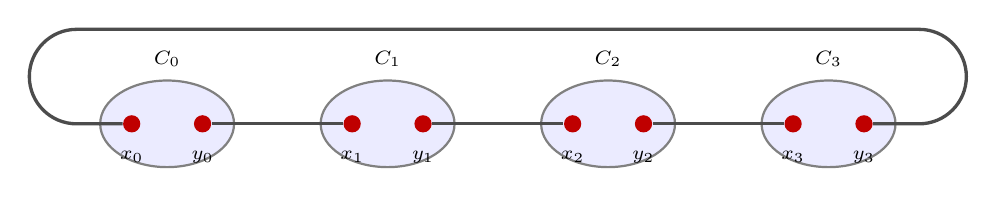
\begin{tikzpicture}[
  site/.style={draw=black!50,fill=blue!8,thick,ellipse,minimum width=1.7cm,minimum height=1.1cm},
  maj/.style={circle,fill=red!75!black,inner sep=2.2pt},
  pair/.style={very thick,black!70},
  lab/.style={font=\scriptsize}]
  \foreach \i/\x in {0/0,1/2.8,2/5.6,3/8.4} {
    \node[site] at (\x,0) {};
    \node[lab,anchor=south] at (\x,0.6) {$C_{\i}$};
    \node[maj] (x\i) at (\x-0.45,0) {};
    \node[maj] (y\i) at (\x+0.45,0) {};
    \node[lab,anchor=north] at ([yshift=-3pt]x\i.south) {$x_{\i}$};
    \node[lab,anchor=north] at ([yshift=-3pt]y\i.south) {$y_{\i}$};
  }
  \draw[pair] (y0) -- (x1);
  \draw[pair] (y1) -- (x2);
  \draw[pair] (y2) -- (x3);
  \draw[pair] (y3) -- ++(0.7,0) arc (-90:90:0.6) -- ++(-10.7,0) arc (90:270:0.6) -- (x0);
\end{tikzpicture}
\caption{The Kitaev chain covariance $K_N$ for $N=4$. Dots are the Majorana labels
$x_i,y_i$ of the physical mode $C_i$, $i\in\mathbb Z/N$; a line joining $y_i$ to $x_{i+1}$ is
the pair $(K_N)_{y_ix_{i+1}}=1$. Every label lies on exactly one line, which is the purity
$K_N^2=-1$.}
\label{fig:kitaev}
\end{figure}

\begin{definition}[Kitaev on-site covariance]\label{def:kitaev}
Let $M=P=1$. $\Gamma_K$ is the matrix on the labels $I_{\mathrm{site}}=(x_A,x_B,x_C,y_A,y_B,y_C)$ with
\[
 (\Gamma_K)_{x_C\,x_A}=1,\qquad(\Gamma_K)_{y_C\,x_B}=1,
\]
their antisymmetric partners $-1$, and every other entry $0$; the rows and columns of
$y_A$ and $y_B$ are zero.
\end{definition}

\begin{lemma}\label{lem:kitaev-adm}
$\Gamma_K$ is admissible and not pure: $\Gamma_K^{\T}=-\Gamma_K$, $1-\Gamma_K^{\T}\Gamma_K$ is
the projector onto $(y_A,y_B)$, and $\Gamma_K^2\neq-1$.
\end{lemma}
\begin{proof}
Antisymmetry is by construction. Each nonzero column of $\Gamma_K$ has a single entry
$\pm1$, and the four nonzero columns $x_A,x_C,x_B,y_C$ are supported on the rows
$x_C,x_A,y_C,x_B$ respectively, so $\Gamma_K^{\T}\Gamma_K=\operatorname{diag}(1,1,1,0,0,1)$ on
$(x_A,x_B,x_C,y_A,y_B,y_C)$ and $1-\Gamma_K^{\T}\Gamma_K$ is the projector onto $(y_A,y_B)$,
positive semidefinite. $\Gamma_K^2=-\Gamma_K^{\T}\Gamma_K\neq-1$.
\end{proof}

\begin{theorem}[The Kitaev chain as a chain with one virtual mode]\label{thm:kitaev}
For every $N\geq1$, with $\Gamma_i=\Gamma_K$ at every site: $\det(1-D\beta_N)=1$ and
\[
 \Gamma_N(\Gamma_K,\ldots,\Gamma_K)=K_N .
\]
$K_N$ is pure and translation invariant, and its momentum-space covariance
(Definition~\ref{def:symbol}) is
\[
 \Sigma(k)=\begin{pmatrix}0&-\omega_k\\ \overline{\omega_k}&0\end{pmatrix}
 \quad\text{on }(x_C,y_C),\qquad k\in\mathbb Z/N .
\]
\end{theorem}
\begin{proof}
\begin{enumerate}
\item[(a)] $\Gamma_K$ has no entry between two virtual labels and none between $x_C$ and
$y_C$, so the retained block $A$ and the eliminated block $D$ of $\Gamma_{\mathrm{in}}$
vanish: $\det(1-D\beta_N)=\det1=1$ and $\Gamma_N=B\beta_NC$. In the labels of
Definition~\ref{def:input}, the only entries of $B$ are
$B_{y_{C_i}x_{B_i}}=(\Gamma_K)_{y_Cx_B}=1$ and $B_{x_{C_i}x_{A_i}}=(\Gamma_K)_{x_Cx_A}=1$,
$C=-B^{\T}$, and $\beta_N$ pairs $x_{A_{i+1}}$ with $x_{B_i}$:
$(\beta_N)_{x_{A_{i+1}}x_{B_i}}=1$ (Definition~\ref{def:periodic}). Each row of $B\beta_NC$
therefore has a single nonzero entry,
\begin{align*}
 (\Gamma_N)_{y_{C_i}\,x_{C_{i+1}}}&=B_{y_{C_i}x_{B_i}}\,(\beta_N)_{x_{B_i}x_{A_{i+1}}}\,C_{x_{A_{i+1}}x_{C_{i+1}}}
 =1\cdot(-1)\cdot(-1)=1,\\
 (\Gamma_N)_{x_{C_{i+1}}\,y_{C_i}}&=B_{x_{C_{i+1}}x_{A_{i+1}}}\,(\beta_N)_{x_{A_{i+1}}x_{B_i}}\,C_{x_{B_i}y_{C_i}}
 =1\cdot1\cdot(-1)=-1,
\end{align*}
which is $K_N$; for $N=1$ the same computation pairs $y_{C_0}$ with $x_{C_0}$ and gives $-\Omega_1$.
\item[(b)] $K_N^2=-1$: every label is paired with exactly one other label, with product of
entries $-1$. The entries depend on $i,j$ only through $j-i$, which is translation
invariance.
\item[(c)] The twisted on-site covariance $\revs{\Gamma_K^{(k)}}$ of Definition~\ref{def:twist} has
$A_k=0$ and $D_k=0$ as in (a), so $\Sigma(k)=B_k\beta_1C_k$. $B_k$ has the entries
$(B_k)_{x_C\,x_A}=1$ and $(B_k)_{y_C\,x_B}=\overline{\omega_k}$ (the twist puts
$\overline{\omega_k}$ on the $x_B$ column), $C_k=-B_k^*$, and $\beta_1$ pairs $x_A$ with
$x_B$ with $(\beta_1)_{x_Ax_B}=1$. Hence
\begin{align*}
 \Sigma(k)_{y_Cx_C}&=(B_k)_{y_Cx_B}(\beta_1)_{x_Bx_A}(C_k)_{x_Ax_C}=\overline{\omega_k}\cdot(-1)\cdot(-1)=\overline{\omega_k},\\
 \Sigma(k)_{x_Cy_C}&=(B_k)_{x_Cx_A}(\beta_1)_{x_Ax_B}(C_k)_{x_By_C}=1\cdot1\cdot(-\omega_k)=-\omega_k,
\end{align*}
and the diagonal entries vanish. \qedhere
\end{enumerate}
\end{proof}

\begin{proposition}[A pure on-site choice closes a virtual loop]\label{prop:loop}
Let $\Gamma'_K$\vet{, the pure completion of $\Gamma_K$,} be $\Gamma_K$ with the additional entries
$(\Gamma'_K)_{y_Ay_B}=-1$, $(\Gamma'_K)_{y_By_A}=1$, which is pure. Then, for the on-site
covariances $\Gamma_i=\Gamma'_K$,
\[
 \det(1-D\beta_N)=2\bigl(1-(-1)^N\bigr)=\begin{cases}4&N\text{ odd}\\0&N\text{ even,}\end{cases}
\]
so the chain covariance is defined only for odd $N$, where it equals $K_N$.
\end{proposition}
\begin{proof}
\begin{enumerate}
\item[(a)] The twisted virtual block of $\Gamma'_K$ has the single pair
$(D_k)_{y_Ay_B}=-\overline{\omega_k}$, $(D_k)_{y_By_A}=\omega_k$, and $\beta_1$ pairs $y_A$
with $y_B$ with entry $-1$; so $1-D_k\beta_1=\operatorname{diag}(1,1,1+\overline{\omega_k},1+\omega_k)$
on $(x_A,x_B,y_A,y_B)$ and $\det(1-D_k\beta_1)=|1+\omega_k|^2$. By
Theorem~\ref{thm:det-factor}, $\det(1-D\beta_N)=\bigl|\prod_k(1+\omega_k)\bigr|^2$.
\item[(b)] The $\omega_k$, $k\in\mathbb Z/N$, are the $N$ distinct $N$-th roots of unity
(they satisfy $\omega_k^N=1$, and $\omega_k=\omega_l$ forces $k=l$ since
$|k-l|<N$), so $z^N-1=\prod_k(z-\omega_k)$; at $z=-1$,
$(-1)^N-1=(-1)^N\prod_k(1+\omega_k)$, that is $\prod_k(1+\omega_k)=1-(-1)^N$. Hence
$\det(1-D\beta_N)=(1-(-1)^N)^2=2(1-(-1)^N)$, as $1-(-1)^N\in\{0,2\}$.
\item[(c)] For odd $N$ every $1-D_k\beta_1$ is invertible, and
$(1-D_k\beta_1)^{-1}=\operatorname{diag}(1,1,(1+\overline{\omega_k})^{-1},(1+\omega_k)^{-1})$ acts as the
identity on the labels $x_A,x_B$, the only virtual labels coupled to $C$; so
$\Sigma(k)=B_k\beta_1(1-D_k\beta_1)^{-1}C_k$ is the matrix of Theorem~\ref{thm:kitaev}(c).
By Theorem~\ref{thm:reconstruct},
$(\Gamma_N)_{(i,y)(j,x)}=\frac1N\sum_k\overline{\chi_k(i)}\,\overline{\omega_k}\,\chi_k(j)
=\frac1N\sum_k\overline{\chi_k(i+1)}\,\chi_k(j)=[\,j=i+1\,]$ by
$\chi_k(i+1)=\chi_k(i)\omega_k$ and orthogonality, likewise
$(\Gamma_N)_{(i,x)(j,y)}=-[\,i=j+1\,]$, and the $(x,x)$ and $(y,y)$ blocks vanish: this is
$K_N$. \qedhere
\end{enumerate}
\end{proof}
The pairs $(y_{A_i},y_{B_i})$ of $\Gamma'_K$ and the bonds $(y_{B_i},y_{A_{i+1}})$ form a
closed loop of Majorana pairs around the ring with no physical label on it, and the
determinant is the product over momenta of the loop's factors $|1+\omega_k|^2$. The three-site family of Section~\ref{sec:chain} contains such a
loop as well: the rotation of $\Gamma_{\mathrm{seed}}$ leaves the pair $(y_A,y_B)$ untouched,
so $D_k\beta_1$ is block diagonal with the same $(y_A,y_B)$ block as in (a),
$\det(1-D_k\beta_1)$ carries the factor $|1+\omega_k|^2$, and the chain determinant of that
family vanishes for even $N$.

\subsection{Hopping gates}
\label{sec:gate}
Fix $n$ modes and two distinct modes $j\neq k$, with the Jordan--Wigner operators $c_a$ of
Definition~\ref{def:majorana}, and $\varphi\in\R$.

\begin{definition}[Hopping gate]\label{def:gate}
\[
 U_{jk}(\varphi)=\bigl(\cos\varphi+\sin\varphi\,c_{x_j}c_{x_k}\bigr)\bigl(\cos\varphi+\sin\varphi\,c_{y_j}c_{y_k}\bigr),
\]
a matrix on $\mathcal F_n$. The rotation $O_{jk}(\varphi)\in\R^{2n\times2n}$ acts on the labels
$(x_j,x_k)$ and on $(y_j,y_k)$ by
\[
 \Rot=\begin{pmatrix}\cos2\varphi&-\sin2\varphi\\
\sin2\varphi&\cos2\varphi\end{pmatrix}
\]
and as the identity on all other labels;
in $(x,y)$ blocks, $O_{jk}(\varphi)=\operatorname{diag}(\Rot_n,\Rot_n)$ with $\Rot_n$ the
rotation by $2\varphi$ in the plane $(j,k)$ of $\R^n$.
\end{definition}
$U_{jk}(\varphi)=\exp\bigl(\varphi\,(c_{x_j}c_{x_k}+c_{y_j}c_{y_k})\bigr)
=\exp\bigl(2\varphi\,(a_j^*a_k-a_k^*a_j)\bigr)$ with
$a_j=\tfrac12(c_{x_j}+\ii c_{y_j})$, the number-conserving hopping gate of angle
$2\varphi$; on covariances the hopping gate is the Givens rotation by $2\varphi$ of the modes
$j,k$ (Theorem~\ref{thm:congruence}). We do not prove the exponential form in these notes.

\begin{theorem}[The hopping gate is a Gaussian unitary]\label{thm:gate}
$U_{jk}(\varphi)$ is unitary, and for every label $a$,
\[
 U_{jk}(\varphi)\,c_a\,U_{jk}(\varphi)^*=\sum_b\bigl(O_{jk}(\varphi)\bigr)_{ab}\,c_b ,
\]
that is, $U c_{x_j}U^*=\cos2\varphi\,c_{x_j}-\sin2\varphi\,c_{x_k}$,
$U c_{x_k}U^*=\sin2\varphi\,c_{x_j}+\cos2\varphi\,c_{x_k}$, the same with $y$, and
$Uc_aU^*=c_a$ for the other labels.
\end{theorem}
\begin{proof}
Let $g=c_{x_j}c_{x_k}$. By Theorem~\ref{thm:car}, $g^2=-1$, $g^*=-g$, $g$ anticommutes with
$c_{x_j}$ and $c_{x_k}$ and commutes with every other $c_a$, including $c_{y_j},c_{y_k}$;
moreover $gc_{x_j}=-c_{x_k}$, $c_{x_j}g=c_{x_k}$, $gc_{x_k}=c_{x_j}$, $c_{x_k}g=-c_{x_j}$.
Hence $V=\cos\varphi+\sin\varphi\,g$ satisfies
$VV^*=(\cos\varphi+\sin\varphi\,g)(\cos\varphi-\sin\varphi\,g)=\cos^2\varphi-\sin^2\varphi\,g^2=1$,
likewise $V^*V=1$, and
\begin{align*}
 Vc_{x_j}V^*&=(\cos\varphi\,c_{x_j}+\sin\varphi\,gc_{x_j})(\cos\varphi-\sin\varphi\,g)
 =(\cos\varphi\,c_{x_j}-\sin\varphi\,c_{x_k})(\cos\varphi-\sin\varphi\,g)\\
 &=(\cos^2\varphi-\sin^2\varphi)\,c_{x_j}-2\sin\varphi\cos\varphi\,c_{x_k}=\cos2\varphi\,c_{x_j}-\sin2\varphi\,c_{x_k};
\end{align*}
similarly $Vc_{x_k}V^*=\sin2\varphi\,c_{x_j}+\cos2\varphi\,c_{x_k}$, and $Vc_aV^*=c_aVV^*=c_a$
for the other labels. The same computation applies to the $y$ factor
$W=\cos\varphi+\sin\varphi\,c_{y_j}c_{y_k}$, which commutes with $c_{x_j},c_{x_k}$; $U=VW$ is unitary as a product of
unitaries, and $Uc_aU^*=V(Wc_aW^*)V^*$ gives the formulas label by label.
\end{proof}

\begin{theorem}[Gaussian unitaries act by orthogonal congruence]\label{thm:congruence}
Let $U$ be unitary and $O\in\R^{2n\times2n}$ with $Uc_aU^*=\sum_bO_{ab}c_b$ for all $a$.
Then $OO^{\T}=1$, and for every density operator $\rho$, $U\rho U^*$ is a density operator with
\[
 \Gamma(U\rho U^*)=O^{\T}\,\Gamma(\rho)\,O .
\]
\end{theorem}
\begin{proof}
\begin{enumerate}
\item[(a)] $\tr(c_ac_b)=2^n\delta_{ab}$: $\tr(c_ac_b)=\tr(c_bc_a)$, so
$2\tr(c_ac_b)=\tr(c_ac_b+c_bc_a)=2\delta_{ab}\tr 1$ (Theorem~\ref{thm:car}).
\item[(b)] $OO^{\T}=1$: $\tr\bigl((Uc_aU^*)(Uc_bU^*)\bigr)=\tr(Uc_ac_bU^*)=\tr(c_ac_b)=2^n\delta_{ab}$,
and by the hypothesis the same trace is
$\sum_{a',b'}O_{aa'}O_{bb'}\tr(c_{a'}c_{b'})=2^n\sum_{a'}O_{aa'}O_{ba'}=2^n(OO^{\T})_{ab}$.
\item[(c)] $U^*c_aU=\sum_bO_{ba}c_b$: conjugating the hypothesis by $U^*$ gives
$c_b=\sum_{b'}O_{bb'}\,U^*c_{b'}U$, and $O^{\T}O=1$ inverts this relation.
\item[(d)] Density: $U\rho U^*\succeq0$ and $\tr(U\rho U^*)=\tr\rho=1$.\linebreak Covariance:
$\Gamma(U\rho U^*)_{ab}=\tfrac\ii2\tr(U\rho U^*[c_a,c_b])$
$=\tfrac\ii2\tr(\rho\,U^*[c_a,c_b]U)$,
and by (c)
\[
 U^*[c_a,c_b]U=[U^*c_aU,U^*c_bU]=\sum_{a'b'}O_{a'a}O_{b'b}[c_{a'},c_{b'}];
\]
taking the trace gives $\sum_{a'b'}O_{a'a}\Gamma(\rho)_{a'b'}O_{b'b}=(O^{\T}\Gamma(\rho)O)_{ab}$,
both sides being real (Theorem~\ref{thm:reality}). \qedhere
\end{enumerate}
\end{proof}

\begin{corollary}[One gate on an occupation state]\label{cor:gate-example}
For $n=2$, $j=1$, $k=2$ and $\rho=|10\rangle\langle10|$,
\[
 \Gamma\bigl(U_{12}(\varphi)\rho U_{12}(\varphi)^*\bigr)
 =\begin{pmatrix}0&X\\-X^{\T}&0\end{pmatrix},\qquad
 X=\begin{pmatrix}\cos4\varphi&-\sin4\varphi\\-\sin4\varphi&-\cos4\varphi\end{pmatrix},
\]
in the labels $(x_1,x_2,y_1,y_2)$. The vacuum is fixed by every hopping gate:
$\Gamma(U_{jk}(\varphi)\,|0\rangle\langle0|\,U_{jk}(\varphi)^*)=-\Omega_n$.
\end{corollary}
\begin{proof}
Theorem~\ref{thm:congruence} with $\Gamma(\rho)=\begin{pmatrix}0&\Lambda_{10}\\-\Lambda_{10}&0\end{pmatrix}$,
$\Lambda_{10}=\operatorname{diag}(1,-1)$ (Theorem~\ref{thm:occupation}), and $O=\operatorname{diag}(\Rot,\Rot)$
with $\Rot$ the rotation by $2\varphi$: the $(x,y)$ block is $\Rot^{\T}\Lambda_{10}\Rot=X$, with
$\cos^22\varphi-\sin^22\varphi=\cos4\varphi$ and $2\sin2\varphi\cos2\varphi=\sin4\varphi$. For
the vacuum, $\Lambda=-1_n$ and $\Rot_n^{\T}(-1)\Rot_n=-1$ since $\Rot_n^{\T}\Rot_n=1$, which follows from
$O^{\T}O=1$.
\end{proof}
A composition of gates acts by the product of the rotations, by
Theorem~\ref{thm:congruence} applied to each factor.

\section{Quadratic Hamiltonians and the realization of covariances}
\label{sec:hamiltonian}
\motiv{Every admissible matrix is the covariance of a density operator
(Theorem~\ref{thm:realization}), the converse of Theorem~\ref{thm:admissible}, and every
quadratic Hamiltonian has a Gaussian ground state (Theorem~\ref{thm:ground-state} \vet{and
Corollary~\ref{cor:families}(c)}). Both rest
on one matrix fact, the normal form $\Gamma=O\,\D(\varepsilon)\,O^{\T}$ of a real
antisymmetric matrix (Theorem~\ref{thm:normal-form}), and on one Fock-space fact, that every
rotation $O$ is implemented by a unitary (Theorem~\ref{thm:implement}).}

Throughout, $n$ modes carry the labels $x_1,\ldots,x_n,y_1,\ldots,y_n$, vectors of $\R^{2n}$
are indexed by the labels, $e_a$ is the unit vector of the label $a$, $u\cdot v$ is the
Euclidean inner product, and $\langle u,v\rangle=\sum_a\overline{u_a}v_a$ is the inner product of
$\C^{2n}$, conjugate-linear in the first argument. For a function $d$ on the configurations $s\in\{0,1\}^n$,
$\operatorname{diag}(d)$ is the matrix on $\mathcal F_n$ with $d(s)$ at the position $(s,s)$
and zero elsewhere. The Majorana operators $c_a$ are those of Definition~\ref{def:majorana},
$\rho$ is a density operator and $\Gamma(\rho)$ its covariance (Definition~\ref{def:density}).
A unitary $U$ \emph{implements} a real matrix $O$ when
$Uc_aU^*=\sum_bO_{ab}c_b$ for every label $a$ ($U$ is the Gaussian unitary, or Bogoliubov
transformation, of the rotation $O$; Theorem~\ref{thm:congruence}); then
$OO^{\T}=1$, $U^*c_aU=\sum_bO_{ba}c_b$, $U^*$ implements $O^{\T}$, and
$\Gamma(U\rho U^*)=O^{\T}\Gamma(\rho)O$, $\Gamma(U^*\rho U)=O\,\Gamma(\rho)\,O^{\T}$.

\subsection{The canonical form and the energy of a quadratic Hamiltonian}
\label{sec:blockform}

\begin{definition}[Canonical form]\label{def:block}
For $\varepsilon\in\R^n$, $\D(\varepsilon)$ is the matrix on the labels with
\[
 \D(\varepsilon)_{x_jy_j}=\varepsilon_j,\qquad \D(\varepsilon)_{y_jx_j}=-\varepsilon_j,
\]
and every other entry $0$; in $(x,y)$ blocks,
$\D(\varepsilon)=\begin{pmatrix}0&\operatorname{diag}(\varepsilon)\\-\operatorname{diag}(\varepsilon)&0\end{pmatrix}$.
\end{definition}
The covariances of Section~\ref{sec:fock} are of this form: $\Omega_n=\D(1,\ldots,1)$
(equation~\eqref{eq:standard}), the vacuum has $\D(-1,\ldots,-1)$, and the occupation state $|s\rangle\langle s|$ has $\D(\nu(s))$ with
$\nu_j(s)=-1$ for $s_j=0$ and $+1$ for $s_j=1$ (Theorem~\ref{thm:occupation}). Since
$\D(\varepsilon)^{\T}\D(\varepsilon)=\operatorname{diag}(\varepsilon^2,\varepsilon^2)$,
$\D(\varepsilon)$ is admissible if and only if $|\varepsilon_j|\leq1$ for all $j$ and pure if and
only if $|\varepsilon_j|=1$ for all $j$.

\begin{definition}[Quadratic Hamiltonian]\label{def:ham}
For a real matrix $h$ on the labels,
\[
 H_h=\frac\ii4\sum_{a,b}h_{ab}\,c_ac_b ,
\]
a matrix on $\mathcal F_n$. The results below assume $h^{\T}=-h$.
\end{definition}
For one mode and $h=\D(\varepsilon)$, $H_h=\tfrac\ii4\varepsilon(c_xc_y-c_yc_x)=\tfrac\ii2\varepsilon\,c_xc_y$;
with $c_x=X$ and $c_y=\ii XZ$ (Definition~\ref{def:majorana}, $n=1$) this is
$-\tfrac12\varepsilon Z=\operatorname{diag}(-\tfrac\varepsilon2,\tfrac\varepsilon2)$ on
$(|0\rangle,|1\rangle)$: the empty mode has energy $-\varepsilon/2$, the filled mode
$+\varepsilon/2$. Lemma~\ref{lem:diagonal} is this computation for $n$ modes.

\begin{lemma}[Hermiticity, energy, conjugation]\label{lem:energy}
Let $h^{\T}=-h$.
\begin{enumerate}
\item[(a)] $H_h^*=H_h$.
\item[(b)] For every Hermitian $\rho$,
$\tr(\rho H_h)=\tfrac14\sum_{a,b}h_{ab}\,\Gamma(\rho)_{ab}$, a real number.
\item[(c)] If the unitary $U$ implements $O$, then $UH_hU^*=H_{O^{\T}hO}$.
\end{enumerate}
\end{lemma}
\begin{proof}
(a) $(c_ac_b)^*=c_bc_a$, so
$H_h^*=-\tfrac\ii4\sum_{ab}h_{ab}c_bc_a=-\tfrac\ii4\sum_{ab}h_{ba}c_ac_b=H_h$.
(b) By Theorem~\ref{thm:car}, $c_ac_b=\delta_{ab}+\tfrac12[c_a,c_b]$; the diagonal terms
carry $h_{aa}=0$, so $\tr(\rho H_h)=\tfrac\ii8\sum_{ab}h_{ab}\tr(\rho[c_a,c_b])
=\tfrac14\sum_{ab}h_{ab}\Gamma(\rho)_{ab}$, real by Theorem~\ref{thm:reality}.
(c) $Uc_ac_bU^*=(Uc_aU^*)(Uc_bU^*)=\sum_{c,d}O_{ac}O_{bd}\,c_cc_d$, hence
$UH_hU^*=\tfrac\ii4\sum_{c,d}\bigl(\sum_{a,b}O_{ac}h_{ab}O_{bd}\bigr)c_cc_d=H_{O^{\T}hO}$.
\end{proof}

\begin{lemma}[The Hamiltonian of a canonical form is diagonal]\label{lem:diagonal}
Let $n_j=\operatorname{diag}(s\mapsto s_j)$ be the number operator of mode $j$. Then
$\ii\,c_{x_j}c_{y_j}=2n_j-1$, and for every $\varepsilon\in\R^n$
\[
 H_{\D(\varepsilon)}=\sum_j\varepsilon_j\bigl(n_j-\tfrac12\bigr)
 =\operatorname{diag}\Bigl(s\mapsto\sum_j\varepsilon_j\bigl(s_j-\tfrac12\bigr)\Bigr).
\]
\end{lemma}
\begin{proof}
$Z_{<j}$ commutes with $X_j$ (Lemma~\ref{lem:pauli}), so
$c_{x_j}c_{y_j}=\ii\,Z_{<j}X_jZ_{<j}X_jZ_j=\ii Z_j$ and
$\ii c_{x_j}c_{y_j}=-Z_j=\operatorname{diag}(-(-1)^{s_j})=2n_j-1$. The only nonzero entries of
$\D(\varepsilon)$ are $\varepsilon_j$ at $(x_j,y_j)$ and $-\varepsilon_j$ at $(y_j,x_j)$, so
$H_{\D(\varepsilon)}=\tfrac\ii4\sum_j\varepsilon_j(c_{x_j}c_{y_j}-c_{y_j}c_{x_j})
=\tfrac\ii2\sum_j\varepsilon_jc_{x_j}c_{y_j}=\tfrac12\sum_j\varepsilon_j(2n_j-1)$.
\end{proof}
\revs{Write $d_\varepsilon(s)=\sum_j\varepsilon_j(s_j-\tfrac12)$ for the diagonal entry of
$H_{\D(\varepsilon)}$ at the configuration $s$.}

\subsection{Ground states of a canonical form}
\label{sec:groundstate}

\begin{lemma}[Ground state of a diagonal operator]\label{lem:diag-min}
Let $d:\{0,1\}^n\to\R$, $D=\operatorname{diag}(d)$, and let $s^\star$ satisfy
$d(s)\geq d(s^\star)$ for all $s$. For every density operator $\rho$,
$\tr(\rho D)=\sum_sd(s)\rho_{ss}\geq d(s^\star)$. If moreover $d(s)>d(s^\star)$ for every
$s\neq s^\star$, then $\tr(\rho D)=d(s^\star)$ implies $\rho=|s^\star\rangle\langle s^\star|$.
\end{lemma}
\begin{proof}
$\rho_{ss}\geq0$ and $\sum_s\rho_{ss}=1$, so
$\tr(\rho D)-d(s^\star)=\sum_s\bigl(d(s)-d(s^\star)\bigr)\rho_{ss}\geq0$. Under the strict
gaps, equality forces $\rho_{ss}=0$ for $s\neq s^\star$. For $\rho\succeq0$ a vanishing
diagonal entry $\rho_{ss}$ forces the row and column $s$ to vanish: the $2\times2$ principal
submatrix on $\{s,t\}$ is positive semidefinite, so $\rho_{ss}\rho_{tt}-|\rho_{st}|^2\geq0$,
that is $\rho_{st}=0$. Hence $\rho=\rho_{s^\star s^\star}|s^\star\rangle\langle s^\star|$, and
$\tr\rho=1$ gives $\rho_{s^\star s^\star}=1$.
\end{proof}

\begin{definition}[Ground configuration and energy of a canonical form]\label{def:ground}
For $\varepsilon\in\R^n$ let $s^\varepsilon\in\{0,1\}^n$ have $s^\varepsilon_j=1$ if
$\varepsilon_j<0$ and $s^\varepsilon_j=0$ otherwise, and let
$\mathcal E_{\mathrm{gs}}(\varepsilon)=-\tfrac12\sum_j|\varepsilon_j|$. With the convention $\sgn0=1$,
$\nu(s^\varepsilon)=-\sgn\varepsilon$ entrywise.
\end{definition}

\begin{theorem}[Ground states of a canonical form]\label{thm:block-gs}
Let $\varepsilon\in\R^n$.
\begin{enumerate}
\item[(a)] For every density operator $\rho$, $\tr(\rho H_{\D(\varepsilon)})\geq \mathcal E_{\mathrm{gs}}(\varepsilon)$,
with equality for $\rho=|s^\varepsilon\rangle\langle s^\varepsilon|$, whose covariance is
$\D(-\sgn\varepsilon)$.
\item[(b)] If $\varepsilon_j\neq0$ for all $j$, then $\tr(\rho H_{\D(\varepsilon)})=\mathcal E_{\mathrm{gs}}(\varepsilon)$
implies $\rho=|s^\varepsilon\rangle\langle s^\varepsilon|$.
\end{enumerate}
\end{theorem}
\begin{proof}
By Lemma~\ref{lem:diagonal}, $H_{\D(\varepsilon)}=\operatorname{diag}(d)$ with
$d(s)=\sum_j\varepsilon_j(s_j-\tfrac12)$. For each $j$, $\varepsilon_j(s_j-s^\varepsilon_j)$
equals $|\varepsilon_j|$ if $s_j\neq s^\varepsilon_j$ and $0$ otherwise. Hence
$d(s)-d(s^\varepsilon)=\sum_{j:\,s_j\neq s^\varepsilon_j}|\varepsilon_j|\geq0$ and
$d(s^\varepsilon)=-\tfrac12\sum_j|\varepsilon_j|$. (a) is Lemma~\ref{lem:diag-min} with
$s^\star=s^\varepsilon$, and the covariance is Theorem~\ref{thm:occupation}. (b) When every
$\varepsilon_j\neq0$ the gap $d(s)-d(s^\varepsilon)$ is positive for $s\neq s^\varepsilon$.
\end{proof}

\begin{theorem}[Ground states of a rotated canonical form]\label{thm:rotated-gs}
Let $h=O\,\D(\varepsilon)\,O^{\T}$ with $OO^{\T}=1$, and let the unitary $U$ implement $O$.
\begin{enumerate}
\item[(a)] For every density operator $\rho$, $\tr(\rho H_h)\geq \mathcal E_{\mathrm{gs}}(\varepsilon)$.
\item[(b)] Equality holds for the pure state
$\rho_{\mathrm{gs}}=U^*|s^\varepsilon\rangle\langle s^\varepsilon|U$, and
$\Gamma(\rho_{\mathrm{gs}})=O\,\D(-\sgn\varepsilon)\,O^{\T}$.
\item[(c)] If $\varepsilon_j\neq0$ for all $j$, then $\tr(\rho H_h)=\mathcal E_{\mathrm{gs}}(\varepsilon)$ implies
$\rho=\rho_{\mathrm{gs}}$.
\end{enumerate}
\end{theorem}
\begin{proof}
By Lemma~\ref{lem:energy}(c) and $O^{\T}O=1$, $UH_hU^*=H_{\D(\varepsilon)}$, so
$\tr(\rho H_h)=\tr\bigl((U\rho U^*)H_{\D(\varepsilon)}\bigr)$ with $U\rho U^*$ a density operator
(Theorem~\ref{thm:congruence}). (a) is Theorem~\ref{thm:block-gs}(a) for $U\rho U^*$.
(b) $U\rho_{\mathrm{gs}}U^*=|s^\varepsilon\rangle\langle s^\varepsilon|$ attains $\mathcal E_{\mathrm{gs}}(\varepsilon)$, and
$\Gamma(U^*\rho U)=O\,\Gamma(\rho)\,O^{\T}$ with
$\Gamma(|s^\varepsilon\rangle\langle s^\varepsilon|)=\D(-\sgn\varepsilon)$. (c)
Theorem~\ref{thm:block-gs}(b) gives $U\rho U^*=|s^\varepsilon\rangle\langle s^\varepsilon|$.
\end{proof}

The energy $\tfrac14\sum_{ab}h_{ab}\Gamma_{ab}$ of Lemma~\ref{lem:energy}(b) is a function of
the covariance alone, and in the frame of $O$ it is a weighted sum of the $(x_j,y_j)$ entries.
\begin{lemma}[Energy in the rotated frame]\label{lem:rotated-form}
Let $h=O\,\D(\varepsilon)\,O^{\T}$ with $OO^{\T}=1$, let $\Gamma^{\T}=-\Gamma$, and put
$\Gamma'=O^{\T}\Gamma O$.
\begin{enumerate}
\item[(a)] $(\Gamma')^{\T}=-\Gamma'$, and $\Gamma'$ is admissible (pure) if and only if $\Gamma$ is.
\item[(b)] $\tfrac14\sum_{a,b}h_{ab}\Gamma_{ab}=\tfrac12\sum_j\varepsilon_j\Gamma'_{x_jy_j}$.
\item[(c)] If $\Gamma=O\,\D(\lambda)\,O^{\T}$, then $\Gamma'=\D(\lambda)$ and
$\tfrac14\sum_{a,b}h_{ab}\Gamma_{ab}=\tfrac12\sum_j\varepsilon_j\lambda_j$.
\end{enumerate}
\end{lemma}
\begin{proof}
(a) $(O^{\T}\Gamma O)^{\T}=O^{\T}\Gamma^{\T}O=-\Gamma'$; admissibility and purity transfer
by Theorem~\ref{thm:orthogonal} in both directions, since $\Gamma=O\Gamma'O^{\T}$.
(b) $\sum_{ab}h_{ab}\Gamma_{ab}=\tr(h^{\T}\Gamma)=\tr(O\D(\varepsilon)^{\T}O^{\T}\Gamma)
=\tr(\D(\varepsilon)^{\T}\Gamma')=\sum_{cd}\D(\varepsilon)_{cd}\Gamma'_{cd}
=\sum_j\varepsilon_j(\Gamma'_{x_jy_j}-\Gamma'_{y_jx_j})=2\sum_j\varepsilon_j\Gamma'_{x_jy_j}$.
(c) $O^{\T}O=1$ gives $\Gamma'=\D(\lambda)$, whose $(x_j,y_j)$ entry is $\lambda_j$.
\end{proof}

\begin{theorem}[The variational bound on covariances]\label{thm:variational}
Let $h=O\,\D(\varepsilon)\,O^{\T}$ with $OO^{\T}=1$, and let $\Gamma$ be admissible. Then
\[
 \tfrac14\sum_{a,b}h_{ab}\Gamma_{ab}\;\geq\;\mathcal E_{\mathrm{gs}}(\varepsilon).
\]
If $\varepsilon_j\neq0$ for all $j$, equality holds if and only if
$\Gamma=O\,\D(-\sgn\varepsilon)\,O^{\T}$.
\end{theorem}
\begin{proof}
Put $\Gamma'=O^{\T}\Gamma O$; by Lemma~\ref{lem:rotated-form}, $\Gamma'$ is admissible and
$\tfrac14\sum h_{ab}\Gamma_{ab}=\tfrac12\sum_j\varepsilon_j\Gamma'_{x_jy_j}$.
Every entry of an admissible matrix has modulus at most $1$, since
$|\Gamma'_{ab}|\leq\|\Gamma'e_b\|\leq1$ (Theorem~\ref{thm:norm-form}). Hence
$\tfrac12\sum_j\varepsilon_j\Gamma'_{x_jy_j}\geq-\tfrac12\sum_j|\varepsilon_j|$,
with equality if and only if $\Gamma'_{x_jy_j}=-\sgn\varepsilon_j$ for every $j$ with
$\varepsilon_j\neq0$. Suppose all $\varepsilon_j\neq0$ and equality holds. Fix $j$. The
column $\Gamma'e_{y_j}$ has norm at most $1$ and the entry $-\sgn\varepsilon_j$ at $x_j$, so
all its other entries vanish; by antisymmetry $\Gamma'_{y_jx_j}=\sgn\varepsilon_j$, and the
same argument on the column $\Gamma'e_{x_j}$ leaves only that entry. Doing this for every
$j$ pins every column of $\Gamma'$, including the entries between different modes, and
gives $\Gamma'=\D(-\sgn\varepsilon)$, that is $\Gamma=O\,\D(-\sgn\varepsilon)\,O^{\T}$.
Conversely this matrix is admissible and has $\Gamma'_{x_jy_j}=-\sgn\varepsilon_j$
(Lemma~\ref{lem:rotated-form}(a),(c)).
\end{proof}

The covariance is linear in the state, so a mode that is occupied with probability
$\tfrac12(1+\lambda_j)$ and empty otherwise contributes the entry $\lambda_j$; a product of
such one-mode mixtures realizes every admissible canonical form.
\begin{definition}[Product mixture]\label{def:mixture}
For $\lambda\in[-1,1]^n$ put $p_j(0)=\tfrac12(1-\lambda_j)$, $p_j(1)=\tfrac12(1+\lambda_j)$,
and $\rho_\lambda=\sum_{s\in\{0,1\}^n}\bigl(\prod_jp_j(s_j)\bigr)|s\rangle\langle s|$.
\end{definition}

\begin{theorem}[Canonical forms are realized by product mixtures]\label{thm:mixture}
For $\lambda\in[-1,1]^n$, $\rho_\lambda$ is a density operator with
$\Gamma(\rho_\lambda)=\D(\lambda)$. If $|\lambda_j|=1$ for all $j$, then
$\rho_\lambda=|s\rangle\langle s|$ with $s_j=1$ if $\lambda_j=1$ and $s_j=0$ if $\lambda_j=-1$.
\end{theorem}
\begin{proof}
The weights are nonnegative and $\sum_s\prod_jp_j(s_j)=\prod_j\bigl(p_j(0)+p_j(1)\bigr)=1$;
a convex combination of density operators is a density operator. The covariance is linear
in $\rho$, so $\Gamma(\rho_\lambda)=\D\bigl(\sum_sp(s)\nu(s)\bigr)$ with $j$-th entry
$\bigl(\sum_bp_j(b)\nu(b)\bigr)\prod_{k\neq j}\bigl(\sum_bp_k(b)\bigr)=-p_j(0)+p_j(1)=\lambda_j$.
If $|\lambda_j|=1$ then $p_j$ is concentrated on one bit and the sum has one term.
\end{proof}

\subsection{The normal form}
\label{sec:normalform}
\motiv{Theorems~\ref{thm:rotated-gs} and~\ref{thm:variational} assume $h$ is a rotation of a
canonical form. Every real antisymmetric matrix is one (Theorem~\ref{thm:normal-form}): the Hermitian
matrix $\ii\Gamma$ has an orthonormal eigenbasis whose real and imaginary parts pair the
labels.}

\begin{theorem}[Real antisymmetric normal form]\label{thm:normal-form}
Let $\Gamma\in\R^{2n\times2n}$ with $\Gamma^{\T}=-\Gamma$. There exist $O$ with $OO^{\T}=1$ and
$\varepsilon\in\R^n$ with $\varepsilon_j\geq0$ such that $\Gamma=O\,\D(\varepsilon)\,O^{\T}$.
\begin{enumerate}
\item[(a)] There also exist such $O,\varepsilon$ with $\det O=1$, one entry of $\varepsilon$
possibly negative.
\item[(b)] For every decomposition $\Gamma=O\D(\varepsilon)O^{\T}$ with $OO^{\T}=1$: if
$\Gamma$ is admissible then $|\varepsilon_j|\leq1$ for all $j$, and if $\Gamma$ is pure
then $|\varepsilon_j|=1$ for all $j$.
\end{enumerate}
\end{theorem}
\begin{proof}
$M=\ii\Gamma$ is Hermitian with $\overline M=-M$. Let $v_1,\ldots,v_{2n}$ be an orthonormal
eigenbasis of $\C^{2n}$, $Mv_k=\mu_kv_k$, $\mu_k\in\R$. Conjugating, $M\overline{v_k}=-\mu_k\overline{v_k}$,
so $\overline{v_k}$ is an eigenvector for $-\mu_k$, and eigenvectors for different eigenvalues
are orthogonal. Let $\mathcal P=\{k:\mu_k>0\}$, and for $k\in\mathcal P$ let $p_k=\sqrt2\,\mathrm{Re}\,v_k$ and
$q_k=-\sqrt2\,\mathrm{Im}\,v_k$, so that $v_k=(p_k-\ii q_k)/\sqrt2$.
\begin{enumerate}
\item[(i)] Pairing. The real and imaginary parts of $\ii\Gamma(p_k-\ii q_k)=\mu_k(p_k-\ii q_k)$
give $\Gamma q_k=\mu_kp_k$ and $\Gamma p_k=-\mu_kq_k$.
\item[(ii)] Orthonormality. For $j,k\in\mathcal P$, $\langle v_j,v_k\rangle=\delta_{jk}$ and
$\langle\overline{v_j},v_k\rangle=0$. In real terms,
$2\langle v_j,v_k\rangle=(p_j\cdot p_k+q_j\cdot q_k)+\ii(q_j\cdot p_k-p_j\cdot q_k)$ and
$2\langle\overline{v_j},v_k\rangle=(p_j\cdot p_k-q_j\cdot q_k)-\ii(p_j\cdot q_k+q_j\cdot p_k)$;
adding and subtracting, $p_j\cdot p_k=q_j\cdot q_k=\delta_{jk}$ and $p_j\cdot q_k=0$. So
$\{p_k,q_k\}_{k\in\mathcal P}$ is orthonormal in $\R^{2n}$ and $|\mathcal P|\leq n$.
\item[(iii)] Completion. Choose an injection $\phi:\mathcal P\to\{1,\ldots,n\}$, place $p_k$ at the
label $x_{\phi(k)}$ and $q_k$ at $y_{\phi(k)}$, and extend to an orthonormal basis
$(b_\ell)_\ell$ of $\R^{2n}$ indexed by the labels.
\item[(iv)] Kernel. Let $x\in\R^{2n}$ be orthogonal to every $p_k,q_k$, $k\in\mathcal P$. Then
$\langle v_k,x\rangle=0$ and $\langle\overline{v_k},x\rangle=0$ for $k\in\mathcal P$. For $\mu_l<0$,
expanding $\overline{v_l}$ in the eigenbasis gives
$\langle\overline{v_l},x\rangle=\sum_k\langle\overline{v_l},v_k\rangle\langle v_k,x\rangle$
with only $k\in\mathcal P$ contributing, so $\langle\overline{v_l},x\rangle=0$ and
$\langle v_l,x\rangle=\overline{\langle\overline{v_l},x\rangle}=0$ ($x$ is real). Hence
$Mx=\sum_l\mu_l\langle v_l,x\rangle v_l=0$, that is $\Gamma x=0$; this applies to every
$b_\ell$ at a label outside the image of $\phi$.
\item[(v)] The matrix. Let $O$ have the columns $b_\ell$, so $OO^{\T}=1$, and let
$\varepsilon_j=\mu_k$ if $j=\phi(k)$ and $\varepsilon_j=0$ otherwise. The entry
$(O^{\T}\Gamma O)_{\ell\ell'}=b_\ell\cdot\Gamma b_{\ell'}$ is determined by the column
$\ell'$: for a kernel label it vanishes by (iv); for $\ell'=y_{\phi(k)}$, $\Gamma b_{\ell'}=\mu_kp_k$
by (i), and $b_\ell\cdot p_k=[\ell=x_{\phi(k)}]$ by the orthonormality of the basis; for
$\ell'=x_{\phi(k)}$, $\Gamma b_{\ell'}=-\mu_kq_k$ and $b_\ell\cdot q_k=[\ell=y_{\phi(k)}]$. Every
label $\ell'$ is of one of the three kinds, so $O^{\T}\Gamma O=\D(\varepsilon)$ entry by entry.
\end{enumerate}
(a) For $n=0$, $O=1$. For $n\geq1$ and $\det O=-1$, let $\mathcal R$ be the reflection of the
label $y_1$; then $O\mathcal R$ is orthogonal with determinant $1$,
$\mathcal R\D(\varepsilon)\mathcal R=\D(\varepsilon')$ with $\varepsilon'_1=-\varepsilon_1$ and
$\varepsilon'_j=\varepsilon_j$ otherwise, and $\Gamma=(O\mathcal R)\D(\varepsilon')(O\mathcal R)^{\T}$.
(b) $\D(\varepsilon)=O^{\T}\Gamma O$ is admissible (pure) with $\Gamma$
(Theorem~\ref{thm:orthogonal}), and the criterion after Definition~\ref{def:block} gives the
bounds.
\end{proof}
For one mode, $\Gamma=\begin{pmatrix}0&\gamma\\-\gamma&0\end{pmatrix}$ and
$\ii\Gamma$ has the eigenvectors $v=(1,-\ii)/\sqrt2$ with eigenvalue $\gamma$ and $\bar v$
with eigenvalue $-\gamma$; for $\gamma>0$ the vectors $p=\sqrt2\,\mathrm{Re}\,v=(1,0)$ and
$q=-\sqrt2\,\mathrm{Im}\,v=(0,1)$ give $O=1$, $\varepsilon=\gamma$; for $\gamma<0$ the
eigenvector for the positive eigenvalue $-\gamma$ is $\bar v=(1,\ii)/\sqrt2$, so $p=(1,0)$,
$q=(0,-1)$, $O=\operatorname{diag}(1,-1)$ and $\varepsilon=-\gamma$; this $O$ has determinant
$-1$, and (a) restores $\det O=1$ by reflecting $y_1$, which returns $O=1$, $\varepsilon=\gamma$.

\subsection{Rotations are implemented by Gaussian unitaries}
\label{sec:rotation}
\motiv{Theorem~\ref{thm:gate} implemented the rotations of two hopping gates. Every rotation
in $SO(2n)$ is a product of plane rotations (Theorem~\ref{thm:givens}), and each plane
rotation is implemented by one factor $\cos\varphi+\sin\varphi\,c_ac_b$
(Lemma~\ref{lem:factor}); hence every rotation is implemented (Theorem~\ref{thm:implement}).}

\begin{definition}[Plane rotations]\label{def:plane}
For labels $a\neq b$ and $(p,q)\in\R^2$ with $p^2+q^2=1$, $\Rot_{ab}(p,q)$ is the matrix on the
labels equal to the identity except for the rows $a$ and $b$, which are $(p,-q)$ and $(q,p)$
on the columns $(a,b)$ (a Givens rotation). A \emph{rotation product} is a finite product of
plane rotations, the empty product being $1$.
\end{definition}
$\Rot_{ab}(p,q)$ is orthogonal with determinant $1$ and $\Rot_{ab}(p,q)^{\T}=\Rot_{ab}(p,-q)$, so
rotation products form a group; a plane rotation of the labels other than $i$, extended by
the identity on $i$, is a plane rotation of all labels. We state the definition and
Theorem~\ref{thm:givens} for an arbitrary finite set of labels, of size $m$.

\begin{theorem}[$SO(m)$ is generated by plane rotations]\label{thm:givens}
Let $O$ be a real matrix on a finite label set of size $m$ with $OO^{\T}=1$ and
$\det O=1$. Then $O$ is a rotation product.
\end{theorem}
\begin{proof}
Induction on $m$. For $m=0$, $O=1$; for $m=1$, $O=(\det O)=(1)$. Let $m\geq2$ and fix a
label $i$.

\emph{Sweep.} For every unit vector $v$ there is a rotation product $W$ of plane rotations
in planes $(a,i)$, $a\neq i$, with $Wv=e_i$. For a set $S$ of labels not containing $i$,
we build a rotation product $W_S$ with $(W_Sv)_a=0$ for all $a\in S$ and, if $S\neq\emptyset$,
$(W_Sv)_i\geq0$, one label at a time: $W_\emptyset=1$; given $W_S$ and a label
$a\notin S\cup\{i\}$, put $w=W_Sv$ and $r=\sqrt{w_a^2+w_i^2}$; if $r=0$ keep $W_S$,
otherwise $W_{S\cup\{a\}}=\Rot_{ai}(w_i/r,\,w_a/r)\,W_S$, since $\Rot_{ai}(w_i/r,w_a/r)$ sends
$(w_a,w_i)$ to $(0,r)$ and fixes the other coordinates. With $S$ the set of all labels
other than $i$, $W_Sv$ has zeros outside $i$, norm $1$ and $(W_Sv)_i\geq0$, so $W_Sv=e_i$.

\emph{Reduction.} Apply the sweep to $v=Oe_i$. Then $\tilde O=WO$ is orthogonal with $\tilde Oe_i=e_i$,
so its column $i$ is $e_i$; the rows of an orthogonal matrix are orthonormal too, and the
row $i$ has $\tilde O_{ii}=1$, so $\tilde O_{ia}=0$ for $a\neq i$. Hence $\tilde O=O'\oplus1$ with $O'$
orthogonal on the labels other than $i$ and $\det O'=\det \tilde O=\det W\,\det O=1$.

\emph{Induction.} By the induction hypothesis $O'$ is a rotation product on $m-1$ labels,
hence so is $\tilde O=O'\oplus1$, and $O=W^{\T}\tilde O$ is a rotation product, $W^{\T}$ being the
product of the transposed plane rotations in reverse order.
\end{proof}

\begin{lemma}[One factor implements one plane rotation]\label{lem:factor}
Let $a\neq b$ and $\varphi\in\R$. The unitary $V=\cos\varphi+\sin\varphi\,c_ac_b$ implements
$\Rot_{ab}(\cos2\varphi,\sin2\varphi)$. For every $(p,q)$ with $p^2+q^2=1$ there is $\varphi$
with $(\cos2\varphi,\sin2\varphi)=(p,q)$. If $U$ implements $O$ and $V$ implements $O'$,
then $UV$ implements $O'O$; the identity implements $1$.
\end{lemma}
\begin{proof}
The conjugation formulas of Theorem~\ref{thm:gate}'s proof, which use only the
anticommutation relations of two distinct labels, are the rows of
$\Rot_{ab}(\cos2\varphi,\sin2\varphi)$: row $a$ is $(\cos2\varphi,-\sin2\varphi)$ on $(a,b)$,
row $b$ is $(\sin2\varphi,\cos2\varphi)$, every other row is a unit vector. For the angle take
$\theta=\arccos p$ if $q\geq0$ and $\theta=-\arccos p$ otherwise, so that $\cos\theta=p$,
$\sin\theta=\pm\sqrt{1-p^2}=q$, and $\varphi=\theta/2$. Product rule:
$(UV)c_a(UV)^*=U\bigl(\sum_bO'_{ab}c_b\bigr)U^*=\sum_d(O'O)_{ad}c_d$.
\end{proof}

\begin{theorem}[Every rotation is implemented by a Gaussian unitary]\label{thm:implement}
For every real matrix $O$ on the Majorana labels with $OO^{\T}=1$ and $\det O=1$ there is a
unitary $U$, a product of factors $\cos\varphi+\sin\varphi\,c_ac_b$, that implements $O$.
\end{theorem}
\begin{proof}
By Theorem~\ref{thm:givens}, $O=\Rot_1\Rot_2\cdots\Rot_T$ with plane rotations $\Rot_t$; by
Lemma~\ref{lem:factor} choose $U_t$ implementing $\Rot_t$; then $U_T\cdots U_2U_1$ implements
$\Rot_1\Rot_2\cdots\Rot_T$ by the product rule.
\end{proof}
\begin{remark}\label{rem:reflections}
We do not implement reflections ($\det O=-1$) here; Theorem~\ref{thm:normal-form}(a) supplies
a decomposition with $\det O=1$.
\end{remark}

\subsection{Realization and ground states}
\label{sec:realization}

\begin{theorem}[Realization of admissible covariances]\label{thm:realization}
Let $\Gamma$ be admissible. Write $\Gamma=O\D(\varepsilon)O^{\T}$ with $\det O=1$ and
$|\varepsilon_j|\leq1$ (Theorem~\ref{thm:normal-form}), and let $U$ implement $O$
(Theorem~\ref{thm:implement}). Then $\rho=U^*\rho_\varepsilon U$ (Definition~\ref{def:mixture})
is a density operator with $\Gamma(\rho)=\Gamma$. If $\Gamma$ is pure then
$\rho=U^*|s\rangle\langle s|U$ with $s_j=1$ if $\varepsilon_j=1$ and $s_j=0$ if
$\varepsilon_j=-1$, a pure state.
\end{theorem}
\begin{proof}
By Theorem~\ref{thm:mixture}, $\rho_\varepsilon$ is a density operator with covariance
$\D(\varepsilon)$; $U^*$ implements $O^{\T}$, so $U^*\rho_\varepsilon U$ is a density operator
with covariance $O\,\D(\varepsilon)\,O^{\T}=\Gamma$ (Theorem~\ref{thm:congruence}). If
$\Gamma$ is pure then $|\varepsilon_j|=1$ and $\rho_\varepsilon=|s\rangle\langle s|$.
\end{proof}
With Theorem~\ref{thm:admissible}: the covariances of density operators on $n$ modes are
exactly the admissible matrices on $2n$ labels, and every pure covariance is the covariance
of a pure state.

\begin{theorem}[Ground state of a quadratic Hamiltonian]\label{thm:ground-state}
Let $h^{\T}=-h$. There exist $O$ with $OO^{\T}=1$, $\det O=1$, $\varepsilon\in\R^n$ with
$h=O\D(\varepsilon)O^{\T}$, and a unitary $U$ implementing $O$; for every such choice
Theorems~\ref{thm:rotated-gs} and~\ref{thm:variational} hold. In particular:
\begin{enumerate}
\item[(a)] $\min\{\tr(\rho H_h):\rho\text{ a density operator}\}$ exists, equals
$-\tfrac12\sum_j|\varepsilon_j|$, and is attained by the pure state
$\rho_{\mathrm{gs}}=U^*|s^\varepsilon\rangle\langle s^\varepsilon|U$, whose covariance
$O\D(-\sgn\varepsilon)O^{\T}$ is pure.
\item[(b)] If $\varepsilon_j\neq0$ for all $j$, the minimizer is unique, and among admissible
matrices the minimizer of $\Gamma\mapsto\tfrac14\sum_{ab}h_{ab}\Gamma_{ab}$ is unique and
equals $\Gamma(\rho_{\mathrm{gs}})$.
\end{enumerate}
\end{theorem}
\begin{proof}
Theorem~\ref{thm:normal-form}(a) and Theorem~\ref{thm:implement} supply $O,\varepsilon,U$;
Theorems~\ref{thm:rotated-gs} and~\ref{thm:variational} give (a) and (b).
\end{proof}
For a Hermitian matrix $M$ write $\sgn(M)$ for the Hermitian matrix with the eigenvectors of
$M$ and the signs of its eigenvalues. When all $\varepsilon_j\neq0$, the ground covariance is
$\Gamma(\rho_{\mathrm{gs}})=\ii\,\sgn(\ii h)$: $\ii h=O\,(\ii\D(\varepsilon))\,O^{\T}$ with $O$ real
orthogonal, so $\sgn(\ii h)=O\,\sgn(\ii\D(\varepsilon))\,O^{\T}$; on the labels of mode $j$,
$(\ii\D(\varepsilon))^2=\varepsilon_j^2\,1$, so $\sgn(\ii\D(\varepsilon))=\ii\D(\sgn\varepsilon)
=-\ii\D(-\sgn\varepsilon)$, and $\sgn(\ii h)=-\ii\,O\D(-\sgn\varepsilon)O^{\T}=-\ii\,\Gamma(\rho_{\mathrm{gs}})$.
The sign in this formula is that of the covariance convention of Definition~\ref{def:density};
with $\Gamma$ defined with the opposite sign, the ground covariance is $-\ii\,\sgn(\ii h)$.

\begin{corollary}[A pure covariance determines the state]\label{cor:pure-determines}
Let $\rho$ be a density operator whose covariance is pure. Write
$\Gamma(\rho)=O\D(\eta)O^{\T}$ with $\det O=1$, $\eta_j=\pm1$ (Theorem~\ref{thm:normal-form}(a),(b)),
and let $U$ implement $O$ (Theorem~\ref{thm:implement}).
Then $\rho=U^*|s\rangle\langle s|U$ with $s_j=1$ if $\eta_j=1$ and $s_j=0$ otherwise. In
particular two density operators with the same pure covariance are equal.
\end{corollary}
\begin{proof}
Let $h=O\D(-\eta)O^{\T}$, so $\varepsilon=-\eta$ has no zero entry, $s^\varepsilon=s$ and
$-\sgn\varepsilon=\eta$. By Lemma~\ref{lem:energy}(b) and Lemma~\ref{lem:rotated-form}(c)
with $\Gamma(\rho)=O\D(\eta)O^{\T}$,
$\tr(\rho H_h)=\tfrac12\sum_j(-\eta_j)\eta_j=-\tfrac n2=\mathcal E_{\mathrm{gs}}(\varepsilon)$, and
Theorem~\ref{thm:rotated-gs}(c) gives $\rho=U^*|s\rangle\langle s|U$.
\end{proof}
\begin{remark}\label{rem:mixed-not-determined}
A covariance that is not pure does not determine the state: for $n=1$, every
$\rho=\tfrac12(1+tX)$ with $|t|\leq1$ has $\Gamma(\rho)=0$, since $c_xc_y=\ii Z$ and
$\tr Z=\tr(XZ)=0$.
\end{remark}

\section{Thermal states and unitary evolution}
\label{sec:thermal}
\motiv{For $h=O\D(\varepsilon)O^{\T}$, the Gibbs state $e^{-H_h}/\tr e^{-H_h}$ of the quadratic
Hamiltonian $H_h$ has covariance $O\,\D(-\tanh(\varepsilon/2))\,O^{\T}$
(Theorem~\ref{thm:thermal}), and the unitary $e^{-\ii tH_h}$ implements the rotation $e^{-th}$
of the Majorana operators (Theorem~\ref{thm:evolution}). Both reduce to the canonical form by
the conjugation $U^*H_{\D(\varepsilon)}U=H_h$ of Section~\ref{sec:hamiltonian}, since
$H_{\D(\varepsilon)}$ is diagonal and we compute its exponentials entrywise.}

The conventions of Section~\ref{sec:hamiltonian} are in force. For a square matrix $A$, real
or complex, $e^A=\sum_{k\geq0}A^k/k!$; we use the facts $e^{\operatorname{diag}(v)}
=\operatorname{diag}(e^{v})$ entrywise, $e^{WAW^{-1}}=We^AW^{-1}$ for invertible $W$,
$e^{A+B}=e^Ae^B$ when $AB=BA$, $(e^A)^*=e^{A^*}$, $(e^A)^{\T}=e^{A^{\T}}$, and
$\tr(WAW^{-1})=\tr A$.

\subsection{The Gibbs family}
\label{sec:exponential-family}

\begin{definition}[Partition function, Gibbs state, thermal state]\label{def:thermal}
For a real matrix $h$ on the labels, the \emph{partition function} and the \emph{Gibbs
state} of $H_h$ are
\[
 \mathcal Z(h)=\tr e^{-H_h},\qquad \rho_h=\mathcal Z(h)^{-1}e^{-H_h},
\]
and for $\tau\in\R$ (the inverse temperature, written $\beta$ in the literature; here
$\beta$ is the bond covariance) the \emph{thermal state} of $H_h$ at inverse temperature
$\tau$ is $\rho_{\tau h}=e^{-\tau H_h}/\tr e^{-\tau H_h}$. The results below assume $h^{\T}=-h$.
\end{definition}
For one mode and $h=\D(\varepsilon)$, $H_h=\operatorname{diag}(-\tfrac\varepsilon2,\tfrac\varepsilon2)$
on $(|0\rangle,|1\rangle)$ (Lemma~\ref{lem:diagonal} for $n=1$), so
$e^{-H_h}=\operatorname{diag}(e^{\varepsilon/2},e^{-\varepsilon/2})$ and $\mathcal Z=2\cosh(\varepsilon/2)$.
Hence $\rho_h=\operatorname{diag}\bigl(\tfrac12(1+\tanh\tfrac\varepsilon2),\tfrac12(1-\tanh\tfrac\varepsilon2)\bigr)$,
and for $\varepsilon>0$ the empty mode has the larger weight, as in the ground state of
Theorem~\ref{thm:block-gs} ($s^\varepsilon_j=0$ for $\varepsilon_j>0$). $\rho_h$ is the thermal state at $\tau=1$; Corollary~\ref{cor:beta} passes to
$\rho_{\tau h}$ by the substitution $\varepsilon\mapsto\tau\varepsilon$.

\begin{lemma}[The Gibbs state of a canonical form]\label{lem:block-exp}
Let $\varepsilon\in\R^n$ and $\lambda_j=-\tanh(\varepsilon_j/2)$. Then
\begin{enumerate}
\item[(a)] $e^{-H_{\D(\varepsilon)}}=\operatorname{diag}\bigl(s\mapsto e^{-d_\varepsilon(s)}\bigr)$;
\item[(b)] $\mathcal Z(\D(\varepsilon))=\prod_j2\cosh(\varepsilon_j/2)$, a positive real number;
\item[(c)] $\rho_{\D(\varepsilon)}=\rho_\lambda$, the product mixture with parameter
$\lambda$; hence $\rho_{\D(\varepsilon)}$ is a density operator with covariance $\D(\lambda)$.
\end{enumerate}
\end{lemma}
\begin{proof}
(a) $-H_{\D(\varepsilon)}=\operatorname{diag}(-d_\varepsilon)$ (Lemma~\ref{lem:diagonal}) and the
exponential of a diagonal matrix is the diagonal matrix of the exponentials of its entries.
(b) $e^{-d_\varepsilon(s)}=\prod_je^{-\varepsilon_j(s_j-1/2)}$, so
\[
 \tr e^{-H_{\D(\varepsilon)}}=\sum_s\prod_je^{-\varepsilon_j(s_j-1/2)}
 =\prod_j\bigl(e^{\varepsilon_j/2}+e^{-\varepsilon_j/2}\bigr)=\prod_j2\cosh(\varepsilon_j/2),
\]
the sum over $s\in\{0,1\}^n$ of a product factorizing over $j$.
(c) By (a) and (b), $\rho_{\D(\varepsilon)}=\sum_sp(s)|s\rangle\langle s|$ with
$p(s)=\prod_je^{-\varepsilon_j(s_j-1/2)}/(2\cosh(\varepsilon_j/2))$. For one factor and
$b\in\{0,1\}$,
\[
 \frac{e^{-\varepsilon(b-1/2)}}{2\cosh(\varepsilon/2)}
 =\frac{\cosh(\varepsilon/2)\mp\sinh(\varepsilon/2)}{2\cosh(\varepsilon/2)}
 =\frac{1\mp\tanh(\varepsilon/2)}2=p_j(b)\quad(\text{sign }-\text{ for }b=1,\ +\text{ for }b=0),
\]
with $p_j$ the Bernoulli weight of parameter $\lambda_j=-\tanh(\varepsilon_j/2)$ of
Definition~\ref{def:mixture}. Hence $p(s)=\prod_jp_j(s_j)$ and
$\rho_{\D(\varepsilon)}=\rho_\lambda$. Theorem~\ref{thm:mixture} gives
the rest.
\end{proof}

\begin{theorem}[The Gibbs family]\label{thm:thermal}
Let $h^{\T}=-h$.
\begin{enumerate}
\item[(a)] Let $h=O\D(\varepsilon)O^{\T}$ with $OO^{\T}=1$ and let the unitary $U$ implement
$O$. Then $\mathcal Z(h)=\prod_j2\cosh(\varepsilon_j/2)$ and
\[
 \rho_h=U^*\rho_{\D(\varepsilon)}U=U^*\rho_\lambda U,\qquad \lambda_j=-\tanh(\varepsilon_j/2),
\]
so $\rho_h$ is a density operator with
$\Gamma(\rho_h)=O\,\D(-\tanh(\varepsilon/2))\,O^{\T}$ and energy
$\tr(\rho_hH_h)=-\tfrac12\sum_j\varepsilon_j\tanh(\varepsilon_j/2)$.
\item[(b)] For every real antisymmetric $h$: $\mathcal Z(h)$ is a positive real number, $\rho_h$ is a
density operator, and there are $O$ with $OO^{\T}=1$, $\det O=1$, and $\varepsilon\in\R^n$ with
$h=O\D(\varepsilon)O^{\T}$ and $\Gamma(\rho_h)=O\,\D(-\tanh(\varepsilon/2))\,O^{\T}$.
\end{enumerate}
\end{theorem}
\begin{proof}
(a) $U^*H_{\D(\varepsilon)}U=H_h$ (proof of Theorem~\ref{thm:rotated-gs}) and $U^*=U^{-1}$, so
$e^{-H_h}=U^*e^{-H_{\D(\varepsilon)}}U$ and $\mathcal Z(h)=\tr e^{-H_{\D(\varepsilon)}}=\mathcal Z(\D(\varepsilon))$ by
Lemma~\ref{lem:block-exp}(b). Hence $\rho_h=U^*\rho_{\D(\varepsilon)}U=U^*\rho_\lambda U$ by
Lemma~\ref{lem:block-exp}(c), which is \vet{the state built in the proof of Theorem~\ref{thm:realization}
(the proof uses only that $U$ implements $O$, not $\det O=1$)} for the
admissible matrix $O\D(\lambda)O^{\T}$: a density operator with covariance $O\D(\lambda)O^{\T}$.
For the energy, Lemma~\ref{lem:energy}(b) and Lemma~\ref{lem:rotated-form}(c) with
$\Gamma(\rho_h)=O\D(\lambda)O^{\T}$ give
$\tr(\rho_hH_h)=\tfrac14\sum_{ab}h_{ab}\Gamma(\rho_h)_{ab}
=\tfrac12\sum_j\varepsilon_j\lambda_j=-\tfrac12\sum_j\varepsilon_j\tanh(\varepsilon_j/2)$.
(b) Theorem~\ref{thm:normal-form}(a) and Theorem~\ref{thm:implement} supply $O$, $\varepsilon$,
$U$; apply (a).
\end{proof}

\begin{corollary}[Thermal states]\label{cor:beta}
Let $h=O\D(\varepsilon)O^{\T}$ with $OO^{\T}=1$, $U$ implementing $O$, and $\tau\in\R$.
The thermal state $\rho_{\tau h}$ is a density operator with
\[
 \Gamma(\rho_{\tau h})=O\,\D\bigl(-\tanh(\tau\varepsilon/2)\bigr)\,O^{\T}
 \qquad\text{and}\qquad
 \tr(\rho_{\tau h}H_h)=-\tfrac12\sum_j\varepsilon_j\tanh(\tau\varepsilon_j/2).
\]
For $h=0$ (or $\tau=0$) the thermal state is $2^{-n}\,1$, with covariance $\Gamma(2^{-n}1)=0$.
\end{corollary}
\begin{proof}
$\tau h=O\D(\tau\varepsilon)O^{\T}$, and Theorem~\ref{thm:thermal}(a) applies. The energy is
\[
 \tfrac14\sum_{ab}h_{ab}\Gamma_{ab}=\tfrac12\sum_j\varepsilon_j\bigl(-\tanh(\tau\varepsilon_j/2)\bigr)
\]
by Lemma~\ref{lem:rotated-form}(c) with $\Gamma(\rho_{\tau h})=O\D(-\tanh(\tau\varepsilon/2))O^{\T}$. For $h=0$: $H_0=0$, $e^0=1$, $\mathcal Z(0)=2^n$, and
Theorem~\ref{thm:thermal}(a) with $O=1$, $U=1$, $\varepsilon=0$ gives $\Gamma(2^{-n}1)=\D(0)=0$.
\end{proof}
\begin{remark}\label{rem:zero-temperature}
As $\tau\to\infty$, $-\tanh(\tau\varepsilon_j/2)\to-\sgn\varepsilon_j$ for every
$\varepsilon_j\neq0$, so \vet{when every $\varepsilon_j\neq0$} the thermal covariance tends entrywise to the ground covariance
$O\D(-\sgn\varepsilon)O^{\T}$ of Theorem~\ref{thm:rotated-gs} and the energy to the ground
energy $-\tfrac12\sum_j|\varepsilon_j|$. For $h=\D(\varepsilon)$ with all $\varepsilon_j>0$ the
limit is the vacuum covariance $-\Omega_n$ of Corollary~\ref{cor:vacuum}.
\end{remark}

\begin{proposition}[Strict admissibility]\label{prop:strict}
Call $\Gamma$ \emph{strictly admissible} when $\Gamma^{\T}=-\Gamma$ and $1-\Gamma^{\T}\Gamma\succ0$
(positive definite). For $h^{\T}=-h$:
\begin{enumerate}
\item[(a)] $\Gamma(\rho_h)$ is strictly admissible;
\item[(b)] if $n\geq1$, $\Gamma(\rho_h)$ is not pure;
\item[(c)] $O\Gamma O^{\T}$ is strictly admissible with $\Gamma$ when $OO^{\T}=1$, and
$\D(\lambda)$ is strictly admissible if and only if $|\lambda_j|<1$ for all $j$.
\end{enumerate}
\end{proposition}
\begin{proof}
(c) $1-(O\Gamma O^{\T})^{\T}(O\Gamma O^{\T})=O(1-\Gamma^{\T}\Gamma)O^{\T}$, and $M\mapsto OMO^{\T}$
preserves positive definiteness for invertible $O$;
$1-\D(\lambda)^{\T}\D(\lambda)=\operatorname{diag}(1-\lambda^2,1-\lambda^2)$ is positive definite
if and only if every $1-\lambda_j^2>0$. (a) By Theorem~\ref{thm:thermal}(b),
$\Gamma(\rho_h)=O\D(\lambda)O^{\T}$ with $|\lambda_j|=|{-\tanh(\varepsilon_j/2)}|<1$; apply (c).
(b) If $\Gamma(\rho_h)$ were pure, $\D(\lambda)=O^{\T}\Gamma(\rho_h)O$ would be pure
(Theorem~\ref{thm:orthogonal} with $O^{\T}$, since $OO^{\T}=1$ gives $O^{\T}O=1$), forcing
$|\lambda_j|=1$ for every $j$; with $n\geq1$ there is a $j$, and $|\lambda_j|<1$ by (a), a
contradiction. Hence $\Gamma(\rho_h)$ is not pure.
\end{proof}
\begin{remark}\label{rem:coordinate-free}
In the normal form, $(\ii\D(\varepsilon))^2=\operatorname{diag}(\varepsilon^2,\varepsilon^2)$,
so for an odd function $f$ the matrix function $f(\ii\D(\varepsilon))$ of the Hermitian matrix
$\ii\D(\varepsilon)$ is $\ii\D(f(\varepsilon))$. Theorem~\ref{thm:thermal} therefore reads
$\Gamma(\rho_h)=\ii\tanh(\ii h/2)$, and Theorem~\ref{thm:exp-realization}(a) reads
$h=2\ii\,\artanh(\ii\Gamma(\rho_h))$: the coordinate-free form of the two theorems.
\end{remark}

\begin{theorem}[Realization by the Gibbs family]\label{thm:exp-realization}
\begin{enumerate}
\item[(a)] Let $\Gamma=O\D(\eta)O^{\T}$ with $OO^{\T}=1$, $|\eta_j|<1$ for all $j$, and let $U$
implement $O$. Put $\varepsilon_j=-2\artanh(\eta_j)$ and $h=O\D(\varepsilon)O^{\T}$. Then
$h^{\T}=-h$ and $\Gamma(\rho_h)=\Gamma$.
\item[(b)] Every strictly admissible $\Gamma$ is the covariance of a Gibbs state:
there is $h$ with $h^{\T}=-h$ and $\Gamma(\rho_h)=\Gamma$.
\item[(c)] (Uniqueness of the parameter in a frame.) Let $OO^{\T}=1$, $U$ implement $O$, and
$\varepsilon,\varepsilon'\in\R^n$. If
$\Gamma(\rho_{O\D(\varepsilon)O^{\T}})=\Gamma(\rho_{O\D(\varepsilon')O^{\T}})$ then
$\varepsilon=\varepsilon'$.
\end{enumerate}
\end{theorem}
\begin{proof}
(a) $\D(\varepsilon)^{\T}=-\D(\varepsilon)$ gives $h^{\T}=-h$. By Theorem~\ref{thm:thermal}(a),
\[
 \Gamma(\rho_h)=O\D(-\tanh(-\artanh\eta))O^{\T}=O\D(\eta)O^{\T},
\]
since $\tanh$ is odd and $\tanh(\artanh x)=x$ for $|x|<1$. (b) Theorem~\ref{thm:normal-form}(a) gives
$\Gamma=O\D(\eta)O^{\T}$ with $OO^{\T}=1$, $\det O=1$; $\D(\eta)=O^{\T}\Gamma O$ is strictly
admissible by Proposition~\ref{prop:strict}(c), so $|\eta_j|<1$; Theorem~\ref{thm:implement}
gives $U$; apply (a). (c) Theorem~\ref{thm:thermal}(a) gives
$O\D(\lambda)O^{\T}=O\D(\lambda')O^{\T}$ with $\lambda_j=-\tanh(\varepsilon_j/2)$,
$\lambda'_j=-\tanh(\varepsilon'_j/2)$; multiplying by $O^{\T}$ on the left and $O$ on the right
($O^{\T}O=1$), $\D(\lambda)=\D(\lambda')$, so $\lambda=\lambda'$ (the entries $x_jy_j$), and
$\tanh$ is injective.
\end{proof}
Uniqueness of the Gibbs state with a given covariance, beyond the fixed frame of (c), is
Corollary~\ref{cor:converse}(c).

\subsection{Unitary evolution}
\label{sec:evolution}
\motiv{In the canonical form the unitary $e^{-\ii tH_{\D(\varepsilon)}}$ is diagonal with the phases
$e^{-\ii td_\varepsilon(s)}$, a product of the factors $\cos\varphi_j+\sin\varphi_j\,c_{x_j}c_{y_j}$
of Lemma~\ref{lem:factor} with $\varphi_j=t\varepsilon_j/2$, and it rotates each plane
$(x_j,y_j)$ by the angle $t\varepsilon_j$ (Lemma~\ref{lem:block-evolution}). For
$h=O\D(\varepsilon)O^{\T}$ the conjugation by $U$ turns this into the rotation $e^{-th}$
(Theorem~\ref{thm:evolution}), so a covariance evolves as $\Gamma\mapsto e^{th}\Gamma e^{-th}$
and the Gibbs states are stationary (Corollary~\ref{cor:stationary}).}

\begin{definition}[Evolution operator, rotation of the planes]\label{def:evolution}
For a real matrix $h$ on the labels and $t\in\R$, $U_h(t)=e^{-\ii tH_h}$. For $\theta\in\R^n$,
$\Rot(\theta)$ is the matrix on the labels written in $(x,y)$ blocks as
\[
 \Rot(\theta)=\begin{pmatrix}\operatorname{diag}(\cos\theta)&-\operatorname{diag}(\sin\theta)\\
 \operatorname{diag}(\sin\theta)&\operatorname{diag}(\cos\theta)\end{pmatrix},
\]
that is, the rows $x_j$ and $y_j$ are $(\cos\theta_j,-\sin\theta_j)$ and
$(\sin\theta_j,\cos\theta_j)$ on the columns $(x_j,y_j)$ and zero elsewhere: the product
of the plane rotations $\Rot_{x_jy_j}(\cos\theta_j,\sin\theta_j)$ of Definition~\ref{def:plane}
over $j$.
\end{definition}

\begin{lemma}[Unitarity and the group law]\label{lem:unitary}
Let $h^{\T}=-h$ and $t,t'\in\R$. Then $U_h(t)^*=U_h(-t)$, $U_h(t)U_h(t)^*=U_h(t)^*U_h(t)=1$,
$U_h(t)U_h(t')=U_h(t+t')$ and $U_h(0)=1$.
\end{lemma}
\begin{proof}
$H_h^*=H_h$ (Lemma~\ref{lem:energy}(a)), so $(-\ii tH_h)^*=\ii tH_h$ and
$U_h(t)^*=e^{\ii tH_h}=U_h(-t)$. The exponents $-\ii tH_h$ and $-\ii t'H_h$ commute, so
$U_h(t)U_h(t')=e^{-\ii(t+t')H_h}=U_h(t+t')$; with $t'=-t$ this gives $U_h(t)U_h(t)^*=U_h(0)=e^0=1$,
and the other order likewise.
\end{proof}

\begin{lemma}[The exponential of a canonical form is a rotation]\label{lem:block-rot}
For $\theta\in\R^n$, $e^{\D(\theta)}=\Rot(-\theta)$; hence $e^{-t\D(\varepsilon)}=\Rot(t\varepsilon)$
for $t\in\R$, $\varepsilon\in\R^n$. Moreover $\Rot(\theta)\Rot(\theta)^{\T}=1$ and
$\Rot(\theta)^{\T}=\Rot(-\theta)$.
\end{lemma}
\begin{proof}
Let $\Upsilon=\operatorname{diag}(\theta,\theta)$, the block-diagonal matrix with $\theta_j$ at $x_j$
and at $y_j$. Then $\D(\theta)^2=-\Upsilon^2$ and $\Upsilon$ commutes with $\D(\theta)$, so for $m\geq0$
\[
 \D(\theta)^{2m}=(-1)^m\Upsilon^{2m}=(-1)^m\operatorname{diag}(\theta^{2m},\theta^{2m}),\quad
 \D(\theta)^{2m+1}=(-1)^m\Upsilon^{2m}\D(\theta)=(-1)^m\D(\theta^{2m+1}),
\]
by induction on $m$, with $\theta^{k}$ entrywise. The exponential series converges
absolutely, so we may split it into its even and odd terms:
\[
 e^{\D(\theta)}=\sum_{m\geq0}\frac{(-1)^m}{(2m)!}\operatorname{diag}(\theta^{2m},\theta^{2m})
 +\sum_{m\geq0}\frac{(-1)^m}{(2m+1)!}\D(\theta^{2m+1}).
\]
Both sums are entrywise: the first is $\operatorname{diag}(\cos\theta,\cos\theta)$ and the
second is $\D(\sin\theta)$, by the series $\cos x=\sum_m(-1)^mx^{2m}/(2m)!$ and
$\sin x=\sum_m(-1)^mx^{2m+1}/(2m+1)!$ applied to each $\theta_j$ (the maps
$v\mapsto\operatorname{diag}(v,v)$ and $v\mapsto\D(v)$ are linear and continuous, so they
commute with the sums). Hence $e^{\D(\theta)}$ has the blocks $\operatorname{diag}(\cos\theta)$,
$\operatorname{diag}(\sin\theta)$, $-\operatorname{diag}(\sin\theta)$,
$\operatorname{diag}(\cos\theta)$, which is $\Rot(-\theta)$; and
$e^{-t\D(\varepsilon)}=e^{\D(-t\varepsilon)}=\Rot(t\varepsilon)$. The block products
$\Rot(\theta)\Rot(\theta)^{\T}$ have the diagonal blocks
$\operatorname{diag}(\cos^2\theta+\sin^2\theta)=1$ and the off-diagonal blocks
$\operatorname{diag}(-\cos\theta\sin\theta+\sin\theta\cos\theta)=0$;
$\Rot(\theta)^{\T}=\Rot(-\theta)$ by inspection of the blocks.
\end{proof}
For one mode, $\D(\theta)=\begin{pmatrix}0&\theta\\-\theta&0\end{pmatrix}$ and
$e^{\D(\theta)}=\begin{pmatrix}\cos\theta&\sin\theta\\-\sin\theta&\cos\theta\end{pmatrix}$,
the rotation of the plane $(x,y)$ by the angle $-\theta$.

\begin{lemma}[Evolution in the canonical form]\label{lem:block-evolution}
Let $\varepsilon\in\R^n$, $t\in\R$, and $\varphi_j=t\varepsilon_j/2$. Then
\[
 U_{\D(\varepsilon)}(t)=\operatorname{diag}\bigl(s\mapsto e^{-\ii t\,d_\varepsilon(s)}\bigr)
 =\operatorname{diag}\Bigl(s\mapsto\prod_je^{\ii\varphi_j(-1)^{s_j}}\Bigr),
\]
and $U_{\D(\varepsilon)}(t)$ implements $\Rot(t\varepsilon)$: for every $j$,
\[
 U\,c_{x_j}U^*=\cos(t\varepsilon_j)\,c_{x_j}-\sin(t\varepsilon_j)\,c_{y_j},\qquad
 U\,c_{y_j}U^*=\sin(t\varepsilon_j)\,c_{x_j}+\cos(t\varepsilon_j)\,c_{y_j},
\]
with $U=U_{\D(\varepsilon)}(t)$.
\end{lemma}
\begin{proof}
$-\ii tH_{\D(\varepsilon)}=\operatorname{diag}(-\ii t\,d_\varepsilon)$ (Lemma~\ref{lem:diagonal}),
whose exponential is the diagonal of the entrywise exponentials; and
$d_\varepsilon(s)=-\tfrac12\sum_j\varepsilon_j(-1)^{s_j}$ since $s_j-\tfrac12=-\tfrac12(-1)^{s_j}$,
so $e^{-\ii td_\varepsilon(s)}=\prod_je^{\ii\varphi_j(-1)^{s_j}}$.
Write $f(s)$ for this entry and $G=\operatorname{diag}(f)$; $|f(s)|=1$, so
$G^*=\operatorname{diag}(\bar f)$. Fix $j$. The diagonal matrices $G$, $G^*$, $Z_{<j}$, $Z_j$
commute with one another, and $GX_j=X_j\operatorname{diag}(f\circ\mathrm{flip}_j)$
(Lemma~\ref{lem:pauli}(c), read from right to left). Hence
\begin{gather*}
 Gc_{x_j}G^*=Z_{<j}\,GX_jG^*=Z_{<j}X_j\,\operatorname{diag}\bigl((f\circ\mathrm{flip}_j)\,\bar f\bigr),\\
 Gc_{y_j}G^*=\ii Z_{<j}\,GX_jG^*\,Z_j=c_{y_j}\,\operatorname{diag}\bigl((f\circ\mathrm{flip}_j)\,\bar f\bigr)
\end{gather*}
(in the second, the diagonal factor commutes with $Z_j$). Now
$f(\mathrm{flip}_js)\overline{f(s)}=e^{\ii\varphi_j((-1)^{s_j+1}-(-1)^{s_j})}=e^{-2\ii\varphi_j(-1)^{s_j}}$,
so $\operatorname{diag}((f\circ\mathrm{flip}_j)\bar f)=\cos2\varphi_j-\ii\sin2\varphi_j\,Z_j$.
Therefore
\[
 Gc_{x_j}G^*=\cos2\varphi_j\,c_{x_j}-\ii\sin2\varphi_j\,c_{x_j}Z_j
 =\cos2\varphi_j\,c_{x_j}-\sin2\varphi_j\,c_{y_j},
\]
using $c_{x_j}Z_j=Z_{<j}X_jZ_j=-\ii c_{y_j}$, and
\[
 Gc_{y_j}G^*=\cos2\varphi_j\,c_{y_j}-\ii\sin2\varphi_j\,c_{y_j}Z_j
 =\cos2\varphi_j\,c_{y_j}+\sin2\varphi_j\,c_{x_j},
\]
using $c_{y_j}Z_j=\ii Z_{<j}X_jZ_jZ_j=\ii c_{x_j}$. With $2\varphi_j=t\varepsilon_j$ these are the
rows $x_j$ and $y_j$ of $\Rot(t\varepsilon)$.
\end{proof}
Equivalently, $U_{\D(\varepsilon)}(t)=\prod_j(\cos\varphi_j+\sin\varphi_j\,c_{x_j}c_{y_j})$, since
$c_{x_j}c_{y_j}=\ii Z_j$ and each factor is $\operatorname{diag}(e^{\ii\varphi_j(-1)^{s_j}})$;
Lemma~\ref{lem:factor} then gives the same rotation.

\begin{theorem}[Unitary evolution is a rotation]\label{thm:evolution}
Let $h^{\T}=-h$ and $t\in\R$.
\begin{enumerate}
\item[(a)] $U_h(t)$ implements $e^{-th}$: $U_h(t)\,c_a\,U_h(t)^*=\sum_b(e^{-th})_{ab}c_b$ for
every label $a$. If $h=O\D(\varepsilon)O^{\T}$ with $OO^{\T}=1$ and $U$ implements $O$, then
$U_h(t)=U^*U_{\D(\varepsilon)}(t)U$ and $e^{-th}=O\Rot(t\varepsilon)O^{\T}$.
\item[(b)] (Heisenberg picture.) $U_h(t)^*\,c_a\,U_h(t)=\sum_b(e^{th})_{ab}c_b$.
\item[(c)] For every density operator $\sigma$, the operator $U_h(t)\sigma U_h(t)^*$ is a
density operator with covariance $e^{th}\,\Gamma(\sigma)\,e^{-th}$.
\item[(d)] (Generator.) $\ii[H_h,c_a]=\sum_bh_{ab}c_b$ for every label $a$.
\end{enumerate}
\end{theorem}
\begin{proof}
(a) Theorem~\ref{thm:normal-form}(a) and Theorem~\ref{thm:implement} supply
$h=O\D(\varepsilon)O^{\T}$, $OO^{\T}=1$, $\det O=1$, and $U$ implementing $O$; fix any such data.
$U^*H_{\D(\varepsilon)}U=H_h$ gives $-\ii tH_h=U^*(-\ii tH_{\D(\varepsilon)})U$, so
$U_h(t)=U^*U_{\D(\varepsilon)}(t)U$. By Lemma~\ref{lem:block-evolution},
$V=U_{\D(\varepsilon)}(t)$ implements $\Rot(t\varepsilon)$; by the product rule of
Lemma~\ref{lem:factor}, $VU$ implements $O\Rot(t\varepsilon)$, and since $U^*$ implements
$O^{\T}$, $U^*(VU)$ implements $O\Rot(t\varepsilon)O^{\T}$. Finally
$O\Rot(t\varepsilon)O^{\T}=Oe^{-t\D(\varepsilon)}O^{\T}=e^{-tO\D(\varepsilon)O^{\T}}=e^{-th}$ by
Lemma~\ref{lem:block-rot} and $O^{\T}=O^{-1}$.
(b) For $U$ implementing $O$, $U^*c_aU=\sum_bO_{ba}c_b$, and
$(e^{-th})_{ba}=\bigl((e^{-th})^{\T}\bigr)_{ab}=(e^{-th^{\T}})_{ab}=(e^{th})_{ab}$.
(c) $U_h(t)$ is unitary (Lemma~\ref{lem:unitary}) and implements $O=e^{-th}$, so
Theorem~\ref{thm:congruence} gives a density operator with covariance
$O^{\T}\Gamma(\sigma)O=e^{th}\Gamma(\sigma)e^{-th}$.
(d) By Theorem~\ref{thm:car},
$[c_bc_c,c_a]=c_b\{c_c,c_a\}-\{c_b,c_a\}c_c=2\delta_{ca}c_b-2\delta_{ba}c_c$, so
$[H_h,c_a]=\tfrac\ii4\sum_{b,c}h_{bc}(2\delta_{ca}c_b-2\delta_{ba}c_c)
=\tfrac\ii2\bigl(\sum_bh_{ba}c_b-\sum_ch_{ac}c_c\bigr)=-\ii\sum_bh_{ab}c_b$,
using $h_{ba}=-h_{ab}$; multiply by $\ii$.
\end{proof}
Parts (b) and (d) together are the Heisenberg equation: differentiating the closed form
$c_a(t)=U_h(t)^*c_aU_h(t)=\sum_b(e^{th})_{ab}c_b$ of (b) gives
$\dot c_a(t)=\sum_bh_{ab}c_b(t)=\ii[H_h,c_a(t)]$, the commutator of (d) at time $t$.

\begin{corollary}[Stationarity of the Gibbs family]\label{cor:stationary}
Let $h^{\T}=-h$ and $t\in\R$. Then $U_h(t)\rho_hU_h(t)^*=\rho_h$, and
$e^{th}\,\Gamma(\rho_h)\,e^{-th}=\Gamma(\rho_h)$.
\end{corollary}
\begin{proof}
$-\ii tH_h$ and $-H_h$ commute, so $e^{-\ii tH_h}e^{-H_h}=e^{-\ii tH_h-H_h}=e^{-H_h}e^{-\ii tH_h}$;
hence $U_h(t)\rho_h=\rho_hU_h(t)$ and $U_h(t)\rho_hU_h(t)^*=\rho_h$ by Lemma~\ref{lem:unitary}.
Theorem~\ref{thm:evolution}(c) applied to $\sigma=\rho_h$ (a density operator by
Theorem~\ref{thm:thermal}(b)) gives the covariance identity.
\end{proof}

\section{Wick's theorem and the Gaussian class}
\label{sec:wick}
\motiv{A state is \emph{Gaussian} when all its Majorana moments are given by Wick's rule
from its covariance. The rotated product mixtures $U^*\rho_\lambda U$ of
Section~\ref{sec:hamiltonian} are Gaussian (Theorem~\ref{thm:mixture-gaussian}), and with
them the Gibbs and thermal states \vet{and the pure states $U^*|s\rangle\langle s|U$}. Since the Majorana monomials form a basis of the
operators on $\mathcal F_n$, a Gaussian state is determined by its covariance
(Theorem~\ref{thm:unique}); hence every Gaussian state is a rotated product mixture, and the
Gibbs state with a given covariance is unique.}

The conventions of Sections~\ref{sec:hamiltonian} and~\ref{sec:thermal} are in force.
Vectors $v\in\C^{2n}$ are indexed by the labels $x_1,\ldots,x_n,y_1,\ldots,y_n$; $e_a$ is the
unit vector of the label $a$, and $v\cdot c=\sum_av_ac_a$. The annihilation operator of mode
$j$ is $a_j=\tfrac12(c_{x_j}+\ii c_{y_j})$, so that $a_j=u\cdot c$ with
$u=\tfrac12(e_{x_j}+\ii e_{y_j})$. For a density operator $\rho$,
$\tr(\rho c_ac_b)=\delta_{ab}-\ii\Gamma(\rho)_{ab}$ (Theorem~\ref{thm:reality} and
$c_ac_b=\delta_{ab}+\tfrac12[c_a,c_b]$), which motivates the \emph{two-point matrix}
\[
 \G(\rho)=1-\ii\,\Gamma(\rho),
\]
a complex matrix on the labels with $\G(\rho)_{ab}=\tr(\rho c_ac_b)$.

\subsection{Wick's rule and the Gaussian class}
\label{sec:gaussian-class}

\begin{definition}[Wick expansion, Gaussian state]\label{def:wick}
For a complex matrix $\G$ on the labels and vectors $v_1,\ldots,v_m\in\C^{2n}$, the
\emph{Wick expansion} is defined by $\W_\G()=1$ and, for $m\geq1$,
\[
 \W_\G(v_1,\ldots,v_m)=\sum_{j=2}^m(-1)^j\,(v_1^{\T}\G v_j)\,
 \W_\G(v_2,\ldots,\widehat{v_j},\ldots,v_m),
\]
where the hat removes the entry. A density operator $\rho$ is \emph{Gaussian} when
\[
 \tr\bigl(\rho\,(v_1\cdot c)(v_2\cdot c)\cdots(v_m\cdot c)\bigr)=\W_{\G(\rho)}(v_1,\ldots,v_m)
 \qquad\text{for all }m\geq0\text{ and all }v_1,\ldots,v_m\in\C^{2n}.
\]
\end{definition}
For $m=1$ the sum is empty and $\W_\G(v_1)=0$; by induction $\W_\G$ vanishes for every odd
$m$. For $m=2$, $\W_\G(v_1,v_2)=v_1^{\T}\G v_2$, and for $m=4$,
\[
 \W_\G(v_1,v_2,v_3,v_4)=(v_1^{\T}\G v_2)(v_3^{\T}\G v_4)-(v_1^{\T}\G v_3)(v_2^{\T}\G v_4)
 +(v_1^{\T}\G v_4)(v_2^{\T}\G v_3),
\]
the sum over pairings with the sign of the pairing. \revf{For every even $m$, $\W_\G(v_1,\ldots,v_m)$ is the Pfaffian
of the antisymmetric $m\times m$ matrix whose entries above the diagonal are
$v_i^{\T}\G v_j$~\cite{bravyi}: the recursion of Definition~\ref{def:wick} is the expansion of
that Pfaffian along its first row.} With $v_i=e_{a_i}$ the rule reads
$\tr(\rho\,c_{a_1}\cdots c_{a_m})=\W_{\G(\rho)}(e_{a_1},\ldots,e_{a_m})$, Wick's rule in its usual
form with the pairing $\tr(\rho c_ac_b)=\delta_{ab}-\ii\Gamma_{ab}$; repeated labels are allowed.
We state the rule for vectors rather than labels because a Gaussian unitary acts on the
vectors, $U(v\cdot c)U^*=(O^{\T}v)\cdot c$ (Theorem~\ref{thm:transport}), and because the
relation that drives Theorem~\ref{thm:mixture-gaussian} involves the combinations
$c_{x_j}\pm\ii\lambda_jc_{y_j}$; the label form is the special case $v_i=e_{a_i}$.

\begin{lemma}[Multilinearity and the two-point rule]\label{lem:wick-basic}
\begin{enumerate}
\item[(a)] $\W_\G(v_1,\ldots,v_m)=0$ for odd $m$, $\W_\G$ is linear in $v_1$, and
$\W_\G(v,w)=v^{\T}\G w$.
\item[(b)] For every density operator $\rho$ and all $v,w$,
$\tr\bigl(\rho\,(v\cdot c)(w\cdot c)\bigr)=v^{\T}\G(\rho)w$; in particular Wick's rule holds
for $m=0$ and $m=2$ for every density operator.
\item[(c)] $(u\cdot c)(w\cdot c)+(w\cdot c)(u\cdot c)=2(u^{\T}w)\,1$ for all $u,w\in\C^{2n}$.
\end{enumerate}
\end{lemma}
\begin{proof}
(a) We noted odd vanishing above; linearity in $v_1$ is linearity of $v_1^{\T}\G v_j$ in each
term; $m=2$ is the definition with one term, $j=2$.
(b) $\tr(\rho(v\cdot c)(w\cdot c))=\sum_{ab}v_aw_b\tr(\rho c_ac_b)=\sum_{ab}v_a\G(\rho)_{ab}w_b$;
for $m=0$ both sides are $\tr\rho=1$.
(c) By Theorem~\ref{thm:car},
$\sum_{ab}u_aw_b(c_ac_b+c_bc_a)=\sum_{ab}u_aw_b\,2\delta_{ab}=2(u^{\T}w)$.
\end{proof}
\begin{remark}\label{rem:wick-condition}
Beyond $m=2$, Wick's rule is a condition. For $n=1$, $\rho=\tfrac12(1+c_{x_1})$ is a
density operator ($c_{x_1}$ is Hermitian with $c_{x_1}^2=1$) with $\tr(\rho c_{x_1})=1\neq0$. For
$n=2$, $M=c_{x_1}c_{y_1}c_{x_2}c_{y_2}$ is Hermitian with $M^2=1$, so
$\rho=\tfrac14(1+M)$ is a density operator; $\Gamma(\rho)=0$ since $c_ac_bM$ is $\pm$ a monomial
of two labels for $a\neq b$ (Lemma~\ref{lem:monomial-trace}), while
$\tr(\rho M)=1\neq0=\W_1(e_{x_1},e_{y_1},e_{x_2},e_{y_2})$. Theorem~\ref{thm:mixture-gaussian}
proves the rule for the product mixtures.
\end{remark}

\begin{theorem}[Transport by a Gaussian unitary]\label{thm:transport}
Let the unitary $U$ implement $O$ and let $\rho$ be a density operator. Then
$U(v\cdot c)U^*=(O^{\T}v)\cdot c$ for every $v$,
$\W_\G(O^{\T}v_1,\ldots,O^{\T}v_m)=\W_{O\G O^{\T}}(v_1,\ldots,v_m)$ for every $\G$, and
$\G(U^*\rho U)=O\,\G(\rho)\,O^{\T}$. If $\rho$ is Gaussian, so is $U^*\rho U$.
\end{theorem}
\begin{proof}
$U(v\cdot c)U^*=\sum_av_a\sum_bO_{ab}c_b=\sum_b(O^{\T}v)_bc_b$. The identity for $\W$ follows
by induction on $m$ from $(O^{\T}v_1)^{\T}\G(O^{\T}v_j)=v_1^{\T}(O\G O^{\T})v_j$. The two-point
matrix transforms with the covariance, $\Gamma(U^*\rho U)=O\Gamma(\rho)O^{\T}$
(Theorem~\ref{thm:congruence}), and $O\,1\,O^{\T}=1$. Finally, with $X=\prod_i(v_i\cdot c)$,
cyclicity of the trace gives
\begin{align*}
 \tr(U^*\rho U\,X)&=\tr(\rho\,UXU^*)=\tr\Bigl(\rho\prod_i\bigl((O^{\T}v_i)\cdot c\bigr)\Bigr)\\
 &=\W_{\G(\rho)}(O^{\T}v_1,\ldots,O^{\T}v_m)=\W_{O\G(\rho)O^{\T}}(v_1,\ldots,v_m),
\end{align*}
which is $\W_{\G(U^*\rho U)}(v_1,\ldots,v_m)$.
\end{proof}

Removing one factor at a time reduces Wick's rule to two identities
(Lemma~\ref{lem:move}) and a criterion (Lemma~\ref{lem:criterion}).

\begin{lemma}[Moving a factor through a product]\label{lem:move}
Let $b=u\cdot c$, $X=(w_1\cdot c)\cdots(w_k\cdot c)$, and let $X_{\hat\imath}$ be the product
with the $i$-th factor removed. Then
\[
 bX=\sum_{i=1}^k(-1)^{i-1}\,2(u^{\T}w_i)\,X_{\hat\imath}+(-1)^kXb,\qquad
 Xb=\sum_{i=1}^k(-1)^{k-i}\,2(u^{\T}w_i)\,X_{\hat\imath}+(-1)^kbX.
\]
\end{lemma}
\begin{proof}
Induction on $k$; for $k=0$ both identities read $b=b$. Write $X=(w_1\cdot c)X'$ with
$X'=(w_2\cdot c)\cdots(w_k\cdot c)$, so that $X_{\hat1}=X'$ and
$X_{\hat\imath}=(w_1\cdot c)X'_{\widehat{i-1}}$ for $i\geq2$. By Lemma~\ref{lem:wick-basic}(c),
$b(w_1\cdot c)=2(u^{\T}w_1)-(w_1\cdot c)b$, so $bX=2(u^{\T}w_1)X'-(w_1\cdot c)\,bX'$; the
induction hypothesis $bX'=\sum_{i=2}^k(-1)^{i-2}2(u^{\T}w_i)X'_{\widehat{i-1}}+(-1)^{k-1}X'b$,
multiplied by $-(w_1\cdot c)$, turns the signs into $(-1)^{i-1}$ and $(-1)^k$ and the products
into $X_{\hat\imath}$ and $Xb$: the first identity. The second is the first solved for $Xb$:
multiply the first identity by $(-1)^k$ and use $(-1)^k(-1)^{i-1}=-(-1)^{k-i}$.
\end{proof}

\begin{lemma}[A recursion criterion]\label{lem:criterion}
Let $\rho$ be a density operator such that (i) $\tr(\rho X)=0$ for every product $X$ of an odd
number of factors $w\cdot c$, and (ii) for every label $a$ and every product
$X=(w_1\cdot c)\cdots(w_k\cdot c)$ with $k$ odd,
\[
 \tr(\rho\,c_aX)=\sum_{i=1}^k(-1)^{i-1}\,\bigl(e_a^{\T}\G(\rho)w_i\bigr)\,\tr(\rho X_{\hat\imath}).
\]
Then $\rho$ is Gaussian.
\end{lemma}
\begin{proof}
We prove Wick's rule by induction on $m$. For $m$ odd both sides vanish, by (i) and
Lemma~\ref{lem:wick-basic}(a). For $m$ even and $m\geq2$, write $v_1\cdot c=\sum_av_{1a}c_a$
and apply (ii) with $X=(v_2\cdot c)\cdots(v_m\cdot c)$, $k=m-1$ odd:
\[
 \tr\bigl(\rho\,(v_1\cdot c)X\bigr)=\sum_av_{1a}\sum_{i=1}^{m-1}(-1)^{i-1}(e_a^{\T}\G w_i)
 \tr(\rho X_{\hat\imath})=\sum_{j=2}^m(-1)^j(v_1^{\T}\G v_j)\,\tr(\rho X_{\widehat{j-1}}),
\]
with $w_i=v_{i+1}$, $j=i+1$, $(-1)^{i-1}=(-1)^j$. By the induction hypothesis
$\tr(\rho X_{\widehat{j-1}})=\W_\G(v_2,\ldots,\widehat{v_j},\ldots,v_m)$, and the right side is
$\W_\G(v_1,\ldots,v_m)$ by Definition~\ref{def:wick}. For $m=0$ both sides are $1$.
\end{proof}

\subsection{The product mixtures are Gaussian}
\label{sec:mixture-gaussian}

\begin{lemma}[Parity]\label{lem:parity}
Let $\Pi_n=Z_1Z_2\cdots Z_n=\operatorname{diag}\bigl(\prod_j(-1)^{s_j}\bigr)$. Then $\Pi_n^2=1$,
$\Pi_nc_a\Pi_n=-c_a$ for every label $a$, and $\Pi_n\rho_\lambda\Pi_n=\rho_\lambda$ for every
$\lambda\in[-1,1]^n$. Consequently $\tr(\rho_\lambda X)=0$ for every product $X$ of an odd number
of factors $w\cdot c$.
\end{lemma}
\begin{proof}
$\Pi_n$ is diagonal with entries $\pm1$, so $\Pi_n^2=1$ and $\Pi_n$ commutes with the diagonal
matrix $\rho_\lambda$. Writing $c_a=\operatorname{diag}(f_a)X_j$ with $j$ the mode of $a$
(equation~\eqref{eq:signed-flip}) and $\pi(s)=\prod_k(-1)^{s_k}$ for the diagonal entry of $\Pi_n$,
$\Pi_nc_a\Pi_n=\operatorname{diag}(\pi\,f_a)X_j\operatorname{diag}(\pi)=\operatorname{diag}(\pi\,f_a\,(\pi\circ\mathrm{flip}_j))X_j$
and $\pi(\mathrm{flip}_js)=-\pi(s)$, so $\Pi_nc_a\Pi_n=-c_a$. For $X$ of odd length,
$\Pi_nX\Pi_n=(-1)^{\text{length}}X=-X$, by induction on the number of factors: $\Pi_n(w\cdot c)X'\Pi_n
=(\Pi_n(w\cdot c)\Pi_n)(\Pi_nX'\Pi_n)=-(w\cdot c)\,\Pi_nX'\Pi_n$. Hence
$\tr(\rho_\lambda X)=\tr(\Pi_n\rho_\lambda\Pi_n\,X)=\tr(\rho_\lambda\,\Pi_nX\Pi_n)=-\tr(\rho_\lambda X)$.
\end{proof}

\begin{lemma}[The mode relation]\label{lem:mode}
Let $\lambda\in[-1,1]^n$ and fix a mode $j$. Then
\[
 (c_{x_j}-\ii\lambda_jc_{y_j})\,\rho_\lambda=\rho_\lambda\,(c_{x_j}+\ii\lambda_jc_{y_j}),\qquad
 (c_{y_j}+\ii\lambda_jc_{x_j})\,\rho_\lambda=\rho_\lambda\,(c_{y_j}-\ii\lambda_jc_{x_j}).
\]
Moreover $\G(\rho_\lambda)=1-\ii\D(\lambda)$ has the rows
$(\G w)_{x_j}=w_{x_j}-\ii\lambda_jw_{y_j}$ and $(\G w)_{y_j}=w_{y_j}+\ii\lambda_jw_{x_j}$ for every
vector $w$.
\end{lemma}
\begin{proof}
$\rho_\lambda=\operatorname{diag}(p)$ with $p(s)=\prod_kp_k(s_k)$ and
$p_j(s_j)=\tfrac12(1-\lambda_j(-1)^{s_j})$ (Definition~\ref{def:mixture}). The factors
$p_k(s_k)$, $k\neq j$, are common to $p(s)$ and $p(\mathrm{flip}_js)$, so
\begin{equation}\label{eq:weight-flip}
 p_j(s_j)\,p(\mathrm{flip}_js)=p_j(1-s_j)\,p(s)\qquad\text{for every }s,
\end{equation}
that is, $(1-\lambda_jZ_j)\operatorname{diag}(p\circ\mathrm{flip}_j)=\rho_\lambda(1+\lambda_jZ_j)$,
since $2p_j(s_j)=1-\lambda_j(-1)^{s_j}$ is the entry of $1-\lambda_jZ_j$ and $2p_j(1-s_j)$ that of
$1+\lambda_jZ_j$. As $Z_{<j}$ is diagonal and $X_j\operatorname{diag}(p)=\operatorname{diag}(p\circ\mathrm{flip}_j)X_j$
(Lemma~\ref{lem:pauli}),
\[
 (1-\lambda_jZ_j)\,c_{x_j}\rho_\lambda=(1-\lambda_jZ_j)Z_{<j}\operatorname{diag}(p\circ\mathrm{flip}_j)X_j
 =\rho_\lambda(1+\lambda_jZ_j)Z_{<j}X_j=\rho_\lambda(1+\lambda_jZ_j)\,c_{x_j}.
\]
Since $Z_jc_{x_j}=-c_{x_j}Z_j=\ii c_{y_j}$ (Lemma~\ref{lem:pauli} and $c_{y_j}=\ii Z_{<j}X_jZ_j$),
$(1\mp\lambda_jZ_j)c_{x_j}=c_{x_j}\mp\ii\lambda_jc_{y_j}$, which is the first identity; the
second is the same computation with $c_{y_j}$ and $Z_jc_{y_j}=-c_{y_j}Z_j=-\ii c_{x_j}$. The
rows of $\G$: $\Gamma(\rho_\lambda)=\D(\lambda)$ (Theorem~\ref{thm:mixture}) has the only
nonzero entries $\pm\lambda_j$ at $(x_j,y_j)$ and $(y_j,x_j)$.
\end{proof}
\begin{remark}\label{rem:kms-row}
For $|\lambda_j|<1$, solving the relation for $c_a\rho_\lambda$ gives the KMS-type form
$c_a\rho_\lambda=\rho_\lambda\sum_b\mathcal K_{ab}c_b$, where on $(x_j,y_j)$
\[
 \mathcal K=\begin{pmatrix}\cosh\varepsilon&-\ii\sinh\varepsilon\\ \ii\sinh\varepsilon&\cosh\varepsilon\end{pmatrix},
\] $\varepsilon=-2\artanh\lambda_j$, the block of $e^{-\ii h}$ for $h=\D(\varepsilon)$;
for $\lambda_j=-1$ it reads $2a_j\rho_\lambda=2\rho_\lambda a_j^*$, both sides zero because the
mode is empty, and for $\lambda_j=1$ the same with $a_j^*$. The single identity covers all
three cases; Theorem~\ref{thm:mixture-gaussian} needs no case distinction.
\end{remark}

\begin{theorem}[The product mixtures are Gaussian]\label{thm:mixture-gaussian}
For every $\lambda\in[-1,1]^n$ the product mixture $\rho_\lambda$ is Gaussian:
$\tr\bigl(\rho_\lambda\prod_i(v_i\cdot c)\bigr)=\W_{1-\ii\D(\lambda)}(v_1,\ldots,v_m)$ for all
$v_1,\ldots,v_m$.
\end{theorem}
\begin{proof}
We apply Lemma~\ref{lem:criterion} with $\rho=\rho_\lambda$ and $\G=\G(\rho_\lambda)=1-\ii\D(\lambda)$.
Condition (i) is Lemma~\ref{lem:parity}. For (ii) fix a mode $j$, a list $w_1,\ldots,w_k$ with
$k$ odd, $X=\prod_i(w_i\cdot c)$, and write $\langle Y\rangle=\tr(\rho_\lambda Y)$,
$A_a=\langle c_aX\rangle$, $B_a=\langle Xc_a\rangle$ and
$r_a=2\sum_i(-1)^{i-1}(w_i)_a\langle X_{\hat\imath}\rangle$ for $a\in\{x_j,y_j\}$.
Lemma~\ref{lem:move} (second identity, $u=e_a$; $k$ odd, so $(-1)^{k-i}=(-1)^{i-1}$) gives
$B_a=r_a-A_a$. Multiplying the first identity of Lemma~\ref{lem:mode} by $X$ on the right and
taking the trace, with $\tr(Y\rho_\lambda X)=\tr(\rho_\lambda XY)$,
\[
 B_{x_j}-\ii\lambda_jB_{y_j}=A_{x_j}+\ii\lambda_jA_{y_j}.
\]
Substituting $B_a=r_a-A_a$ for both labels, the terms $\pm\ii\lambda_jA_{y_j}$ cancel and
\[
 2A_{x_j}=r_{x_j}-\ii\lambda_jr_{y_j}
 =2\sum_i(-1)^{i-1}\bigl((w_i)_{x_j}-\ii\lambda_j(w_i)_{y_j}\bigr)\langle X_{\hat\imath}\rangle
 =2\sum_i(-1)^{i-1}(e_{x_j}^{\T}\G w_i)\langle X_{\hat\imath}\rangle
\]
by the row of $\G$ in Lemma~\ref{lem:mode}: this is (ii) for $a=x_j$. The second identity of
Lemma~\ref{lem:mode} gives in the same way $2A_{y_j}=r_{y_j}+\ii\lambda_jr_{x_j}$, which is (ii)
for $a=y_j$.
\end{proof}

\begin{corollary}[The Gaussian families]\label{cor:families}
\begin{enumerate}
\item[(a)] For $OO^{\T}=1$, $U$ implementing $O$ and $\lambda\in[-1,1]^n$, the state
$U^*\rho_\lambda U$ \vet{(as in the proof of Theorem~\ref{thm:realization}, which does not use $\det O=1$)} is Gaussian with
$\G=O(1-\ii\D(\lambda))O^{\T}$.
\item[(b)] Every Gibbs state $\rho_h$, $h^{\T}=-h$, and every thermal state
$\rho_{\tau h}$ is Gaussian.
\item[(c)] Every occupation state $|s\rangle\langle s|$ and every pure state
$U^*|s\rangle\langle s|U$ with $U$ implementing an orthogonal $O$ is Gaussian.
\end{enumerate}
\end{corollary}
\begin{proof}
(a) Theorems~\ref{thm:mixture-gaussian} and~\ref{thm:transport}. (b) Theorem~\ref{thm:thermal}:
$\rho_h=U^*\rho_\lambda U$ with $\lambda_j=-\tanh(\varepsilon_j/2)$ for a normal form
$h=O\D(\varepsilon)O^{\T}$ and $U$ implementing $O$; apply (a); $\rho_{\tau h}$ is the Gibbs
state of $\tau h$, and $(\tau h)^{\T}=-\tau h$. (c) $|s\rangle\langle s|=\rho_\lambda$ with $\lambda_j=\pm1$
(Theorem~\ref{thm:mixture}); apply (a).
\end{proof}

\subsection{Moments determine the state}
\label{sec:monomials}

\begin{definition}[Majorana monomials]\label{def:monomial}
Order the labels $x_1<\cdots<x_n<y_1<\cdots<y_n$. For a set $S$ of labels, $c_S$ is the product
of the $c_a$, $a\in S$, in increasing order; $c_\emptyset=1$.
\end{definition}

\begin{lemma}[Traces of monomials]\label{lem:monomial-trace}
\begin{enumerate}
\item[(a)] $\tr(c_S)=0$ for $S\neq\emptyset$.
\item[(b)] $c_S^*c_S=1$ and, for $S\neq T$, $c_S^*c_T=\pm c_{S\triangle T}$ with
$S\triangle T\neq\emptyset$ the symmetric difference. Hence $\tr(c_S^*c_T)=2^n[S=T]$.
\end{enumerate}
\end{lemma}
\begin{proof}
(a) If $|S|$ is odd, $\Pi_nc_S\Pi_n=-c_S$ by Lemma~\ref{lem:parity}, so
$\tr c_S=\tr(\Pi_nc_S\Pi_n)=-\tr c_S$. If $|S|\geq2$ is even, write $c_S=c_ac_{S'}$ with $a\in S$
and
$|S'|$ odd; the labels of $S'$ differ from $a$, so $c_{S'}c_a=(-1)^{|S'|}c_ac_{S'}=-c_ac_{S'}$
and $\tr(c_S)=\tr(c_{S'}c_a)=-\tr(c_S)$.
(b) Insertion rule: for a set $T$ of labels and a label $a$,
$c_ac_T=(-1)^{|\{t\in T:t<a\}|}c_{T\cup\{a\}}$ if $a\notin T$ and
$c_ac_T=(-1)^{|\{t\in T:t<a\}|}c_{T\setminus\{a\}}$ if $a\in T$: move $c_a$ to the right past
the factors $c_t$ with $t<a$ (one sign each, Theorem~\ref{thm:car}), where it either takes
its place in the order or meets $c_a$ and cancels by $c_ac_a=1$. Hence, by induction on $|S|$,
$c_Sc_T=\pm c_{S\triangle T}$ for all $S,T$: for $S=\emptyset$ this is $c_T=c_T$; otherwise
write $c_S=c_ac_{S'}$ with $a=\min S$, apply the
hypothesis to $c_{S'}c_T=\pm c_{S'\triangle T}$ and then the insertion rule to
$c_ac_{S'\triangle T}$, noting $S\triangle T=\{a\}\triangle(S'\triangle T)$. Since
$c_S^*=\pm c_S$ (reversing $|S|$ distinct anticommuting factors, $c_a^*=c_a$),
$c_S^*c_T=\pm c_{S\triangle T}$, with $c_S^*c_S=1$ exactly: $c_S^*c_S=c_{a_m}\cdots c_{a_1}c_{a_1}\cdots c_{a_m}$ for
$S=\{a_1<\cdots<a_m\}$, and the innermost pair $c_{a_1}c_{a_1}=1$ cancels, then the next, and
so on. The trace then follows from (a), $S\triangle T\neq\emptyset$ for $S\neq T$, and
$\tr1=2^n$.
\end{proof}

\begin{theorem}[The monomial basis]\label{thm:basis}
The $4^n$ monomials $c_S$ are linearly independent, hence a basis of the $4^n$-dimensional
space of matrices on $\mathcal F_n$, and every matrix $A$ satisfies
\[
 A=2^{-n}\sum_S\tr(Ac_S^*)\,c_S .
\]
In particular, if $\tr(Ac_S)=\tr(Bc_S)$ for all $S$, then $A=B$.
\end{theorem}
\begin{proof}
If $\sum_S\alpha_Sc_S=0$, multiply by $c_T^*$ on the left and take the trace:
$2^n\alpha_T=0$ by Lemma~\ref{lem:monomial-trace}(b). There are $2^{2n}=(2^n)^2$ subsets and
the matrices on the $2^n$-dimensional space $\mathcal F_n$ form a $(2^n)^2$-dimensional space, so the
independent family is a basis. Writing $A=\sum_S\alpha_Sc_S$ and taking
$\tr(Ac_T^*)=\sum_S\alpha_S\tr(c_Sc_T^*)=\sum_S\alpha_S\tr(c_T^*c_S)=2^n\alpha_T$ (cyclicity and
Lemma~\ref{lem:monomial-trace}(b)) gives the formula; the last statement follows since
$c_S^*=\pm c_S$.
\end{proof}

\begin{theorem}[A Gaussian state is determined by its covariance]\label{thm:unique}
If $\rho$ and $\sigma$ are Gaussian and $\Gamma(\rho)=\Gamma(\sigma)$, then $\rho=\sigma$.
\end{theorem}
\begin{proof}
For every $S=\{a_1<\cdots<a_m\}$, $\tr(\rho c_S)=\W_{\G(\rho)}(e_{a_1},\ldots,e_{a_m})$ by
Wick's rule, and $\G(\rho)=1-\ii\Gamma(\rho)=\G(\sigma)$; so $\tr(\rho c_S)=\tr(\sigma c_S)$ for
all $S$ and Theorem~\ref{thm:basis} gives $\rho=\sigma$.
\end{proof}
For an admissible $\Gamma$ write $\rho[\Gamma]$ for the Gaussian state with covariance
$\Gamma$, unique by Theorem~\ref{thm:unique}; it exists by Theorem~\ref{thm:realization} and
Corollary~\ref{cor:families}(a).

\begin{corollary}[Every Gaussian state is a rotated product mixture]\label{cor:converse}
Let $\rho$ be Gaussian with covariance $\Gamma=O\D(\eta)O^{\T}$, $OO^{\T}=1$, $\det O=1$,
$|\eta_j|\leq1$ (Theorem~\ref{thm:normal-form}), and let $U$ implement $O$. Then
\begin{enumerate}
\item[(a)] $\rho=U^*\rho_\eta U$;
\item[(b)] if $\Gamma$ is pure, $\rho=U^*|s\rangle\langle s|U$ with $s_j=[\eta_j=1]$, and
$\rho^2=\rho$;
\item[(c)] if $\Gamma$ is strictly admissible, $\rho=\rho_h$ for some $h^{\T}=-h$; and for
$h^{\T}=-h$, $h'^{\T}=-h'$ with $\Gamma(\rho_h)=\Gamma(\rho_{h'})$, $\rho_h=\rho_{h'}$.
\end{enumerate}
\end{corollary}
\begin{proof}
(a) $U^*\rho_\eta U$ is a density operator with covariance $\Gamma$
(Theorem~\ref{thm:realization}) and is Gaussian (Corollary~\ref{cor:families}(a)); apply
Theorem~\ref{thm:unique}. (b) For pure $\Gamma$, $|\eta_j|=1$ for all $j$
(Theorem~\ref{thm:normal-form}) and $\rho_\eta=|s\rangle\langle s|$ (Theorem~\ref{thm:mixture});
$\rho^2=U^*|s\rangle\langle s|UU^*|s\rangle\langle s|U=\rho$. (c) By
Theorem~\ref{thm:exp-realization} there is $h^{\T}=-h$ with $\Gamma(\rho_h)=\Gamma$; $\rho_h$ is
Gaussian (Corollary~\ref{cor:families}(b)); apply Theorem~\ref{thm:unique}, and likewise for
$\rho_h,\rho_{h'}$.
\end{proof}
\revf{For a pure covariance the Gaussian hypothesis of Theorem~\ref{thm:unique} can be dropped: two
density operators with the same pure covariance are equal (Corollary~\ref{cor:pure-determines}).}

\section{The partial trace, the contraction of states, and the Gaussian fMPS}
\label{sec:gaussianmap}
\motiv{Section~\ref{sec:contraction} defined the contraction $\Gamma\star\beta$ of an input
covariance with a bond covariance and Section~\ref{sec:chain} built the covariance $\Gamma_N$ of a
periodic chain from it. This section performs the contraction on Fock space. Tracing the bond
modes out of $\rho\,(1\otimes\sigma)$, for Gaussian $\rho$ and $\sigma$ \vet{with $1-D\beta$ invertible}, gives a Gaussian state
whose covariance is $\Gamma(\rho)\star\Gamma(\sigma)$ (Theorem~\ref{thm:state-contract}); the
periodic chain is therefore a Gaussian state on Fock space with covariance $\Gamma_N$
(Theorem~\ref{thm:chain-state}). The tool is a single identity satisfied by every Gaussian
state, $(\G^{\T}v\cdot c)\,\rho=\rho\,(\G v\cdot c)$, which characterizes the class among the
density operators with vanishing odd moments.}

The conventions of Section~\ref{sec:wick} are in force. Throughout, we split $n+m$ modes into
the \emph{retained} modes $1,\ldots,n$ and the \emph{eliminated} modes $n+1,\ldots,n+m$; $R$ and $E$
denote their labels, and a matrix on the labels is written in blocks
$\Gamma=\begin{psmallmatrix}A&B\\C&D\end{psmallmatrix}$ with $A$ on $R$ and $D$ on $E$. For a
matrix $\beta$ on $E$ with $1-D\beta$ invertible, $\Gamma\star\beta=A+B\beta(1-D\beta)^{-1}C$
(Definition~\ref{def:contract}); $1-D\beta$ is invertible iff $1-\beta D$ is, since
$\det(1-D\beta)=\det(1-\beta D)$. The parity of $n+m$ modes is $\Pi_{n+m}=Z_1\cdots Z_{n+m}$
(Lemma~\ref{lem:parity}). The blocks are those of Section~\ref{sec:contraction} with the
eliminated labels placed last; the orientation of the bond covariance $\beta$ is the one fixed
in Definition~\ref{def:bond}.

\subsection{The partial trace}
\label{sec:ptrace}

\begin{definition}[Split, tensor product, partial traces]\label{def:ptrace}
Write a configuration $s\in\{0,1\}^{n+m}$ as $(s_R,s_E)$ with $s_R$ its first $n$ and $s_E$ its last
$m$ bits, so that a matrix $M$ on $\mathcal F_{n+m}$ has entries $M_{(s_R,s_E),(t_R,t_E)}$. For $X$ on
$\mathcal F_n$ and $Y$ on $\mathcal F_m$, $(X\otimes Y)_{(s_R,s_E),(t_R,t_E)}=X_{s_Rt_R}Y_{s_Et_E}$.
The \emph{partial trace over $E$} of $M$ is the matrix on $\mathcal F_n$ with
$(\ptr{E}M)_{s_Rt_R}=\sum_uM_{(s_R,u),(t_R,u)}$, and the partial trace over $R$ is the matrix on
$\mathcal F_m$ with $(\ptr{R}M)_{s_Et_E}=\sum_uM_{(u,s_E),(u,t_E)}$.
\end{definition}

\begin{lemma}[Majorana operators of a split]\label{lem:jw}
Write $c^{(n)}_a$ and $c^{(m)}_e$ for the Majorana operators of $\mathcal F_n$ and $\mathcal F_m$.
For a retained label $a$, $c_a=c^{(n)}_a\otimes1$; for an eliminated label $e$ of mode $n+j$,
$c_e=\Pi_n\otimes c^{(m)}_{e'}$ with $e'$ the label of mode $j$ of $\mathcal F_m$. Consequently,
for $v\in\C^{2n}$ extended by zero to $\bar v\in\C^{2(n+m)}$, $\bar v\cdot c=(v\cdot c^{(n)})\otimes1$ and
$\prod_i(\bar v_i\cdot c)=\bigl(\prod_i(v_i\cdot c^{(n)})\bigr)\otimes1$; for $u\in\C^{2m}$
extended by zero to $\bar u$, $\bar u\cdot c=\Pi_n\otimes(u\cdot c^{(m)})$ and
$\prod_{i=1}^k(\bar u_i\cdot c)=\Pi_n^{\,k}\otimes\prod_i(u_i\cdot c^{(m)})$; $\Pi_{n+m}=\Pi_n\otimes\Pi_m$;
and $X\otimes1$ commutes with $1\otimes Y$.
\end{lemma}
\begin{proof}
$X_j$ and $Z_j$ act on bit $j$ alone: for $j\leq n$, $X_j=X^{(n)}_j\otimes1$, $Z_j=Z^{(n)}_j\otimes1$
and $Z_{<j}=Z^{(n)}_{<j}\otimes1$, so $c_a=c^{(n)}_a\otimes1$ by Definition~\ref{def:majorana}. For
$j>n$, $X_j=1\otimes X^{(m)}_{j-n}$, $Z_j=1\otimes Z^{(m)}_{j-n}$ and
$Z_{<j}=Z_1\cdots Z_n\,Z_{n+1}\cdots Z_{j-1}=\Pi_n\otimes Z^{(m)}_{<j-n}$, so
$c_{x_j}=Z_{<j}X_j=\Pi_n\otimes Z^{(m)}_{<j-n}X^{(m)}_{j-n}=\Pi_n\otimes c^{(m)}_{x_{j-n}}$, and likewise for
$c_{y_j}$. The products follow from $(X\otimes Y)(X'\otimes Y')=XX'\otimes YY'$ and $\Pi_n^2=1$, the
parity from $\Pi_{n+m}=Z_1\cdots Z_n\,Z_{n+1}\cdots Z_{n+m}$, and the commutation from
$(X\otimes1)(1\otimes Y)=X\otimes Y=(1\otimes Y)(X\otimes1)$.
\end{proof}

\begin{lemma}[Partial-trace calculus]\label{lem:ptrace}
For matrices $M,M'$ on $\mathcal F_{n+m}$, $X$ on $\mathcal F_n$, and $Y,V$ on $\mathcal F_m$:
\begin{enumerate}
\item[(a)] $\ptr{E}$ is linear, $\tr(\ptr{E}M)=\tr M$, $\ptr{E}(X\otimes Y)=(\tr Y)X$,
$\ptr{E}\bigl((X\otimes1)M\bigr)=X\,\ptr{E}M$, $\ptr{E}\bigl(M(X\otimes1)\bigr)=(\ptr{E}M)X$,
$\ptr{E}\bigl(M(1\otimes V)\bigr)=\ptr{E}\bigl((1\otimes V)M\bigr)$, and
$\tr\bigl((\ptr{E}M)X\bigr)=\tr\bigl(M(X\otimes1)\bigr)$.
\item[(b)] $(\ptr{E}M)^*=\ptr{E}(M^*)$; if $M\succeq0$ then $\ptr{E}M\succeq0$; if $M$ is a density
operator, so is $\ptr{E}M$.
\item[(c)] The same for $\ptr{R}$ with the roles of the two factors exchanged.
\end{enumerate}
\end{lemma}
\begin{proof}
(a) Entrywise from Definition~\ref{def:ptrace}:
\begin{gather*}
 \textstyle\sum_u(X\otimes Y)_{(s,u),(t,u)}=X_{st}\sum_uY_{uu},\qquad
 \bigl((X\otimes1)M\bigr)_{(s,u),(t,u)}=\sum_{s'}X_{ss'}M_{(s',u),(t,u)},\\
 \textstyle\bigl(M(1\otimes V)\bigr)_{(s,u),(t,u)}=\sum_{u'}M_{(s,u),(t,u')}V_{u'u},\qquad
 \bigl((1\otimes V)M\bigr)_{(s,u),(t,u)}=\sum_{u'}V_{uu'}M_{(s,u'),(t,u)},
\end{gather*}
the second summed over $u$, and the last two summed over $u$ both equal
$\sum_{u,u'}M_{(s,u),(t,u')}V_{u'u}$; finally
$\tr((\ptr{E}M)X)=\sum_{s,t,u}M_{(s,u),(t,u)}X_{ts}=\tr(M(X\otimes1))$.
(b) $\overline{(\ptr{E}M)_{ts}}=\sum_u\overline{M_{(t,u),(s,u)}}=\sum_u(M^*)_{(s,u),(t,u)}$. For
$x\in\C^{2^n}$, $x^*(\ptr{E}M)x=\sum_ux_u^*Mx_u$ with $x_u=x\otimes e_u$, and each term is $\geq0$.
The trace is preserved by (a).
\end{proof}

\begin{theorem}[Marginals of a Gaussian state]\label{thm:marginal}
Let $\rho$ be Gaussian on $n+m$ modes with covariance $\begin{psmallmatrix}A&B\\C&D\end{psmallmatrix}$.
Then $\ptr{E}\rho$ is Gaussian on $n$ modes with covariance $A$, and $\ptr{R}\rho$ is Gaussian on
$m$ modes with covariance $D$.
\end{theorem}
\begin{proof}
Both are density operators (Lemma~\ref{lem:ptrace}(b)). For $v_1,\ldots,v_k\in\C^{2n}$ with
extensions $\bar v_i$, Lemmas~\ref{lem:ptrace}(a) and~\ref{lem:jw} give
$\tr\bigl(\ptr{E}\rho\prod_i(v_i\cdot c^{(n)})\bigr)=\tr\bigl(\rho\prod_i(\bar v_i\cdot c)\bigr)
=\W_{\G(\rho)}(\bar v_1,\ldots,\bar v_k)=\W_{1-\ii A}(v_1,\ldots,v_k)$, the last step because
$\bar v_i^{\T}\G(\rho)\bar v_j=v_i^{\T}(1-\ii A)v_j$ and $\W$ depends on its matrix only through
these pairings; and $1-\ii A=\G(\ptr{E}\rho)$ by the two-point rule
(Lemma~\ref{lem:wick-basic}(b)). For $\ptr{R}$ and $u_1,\ldots,u_k\in\C^{2m}$ with extensions
$\bar u_i$: if $k$ is even, $1\otimes\prod_i(u_i\cdot c^{(m)})=\prod_i(\bar u_i\cdot c)$
(Lemma~\ref{lem:jw}), so the moment is $\W_{\G(\rho)}(\bar u)=\W_{1-\ii D}(u)$; if $k$ is odd,
$1\otimes\prod_i(u_i\cdot c^{(m)})=(\Pi_n\otimes1)\prod_i(\bar u_i\cdot c)$, and
$\Pi_n\otimes1=\prod_{j\leq n}(-\ii\,c_{x_j}c_{y_j})$ is a product of $2n$ retained Majorana
operators, so the moment is a moment of $\rho$ of odd length $2n+k$, hence $0=\W_{1-\ii D}(u)$.
\end{proof}

\subsection{The defining relation}
\label{sec:relation}

\begin{theorem}[The defining relation of a Gaussian state]\label{thm:relation}
Let $\rho$ be Gaussian with $\G=\G(\rho)$. Then $(\G^{\T}v\cdot c)\,\rho=\rho\,(\G v\cdot c)$ for
every $v\in\C^{2(n+m)}$, and $\Pi_{n+m}\rho\Pi_{n+m}=\rho$.
\end{theorem}
\begin{proof}
By Corollary~\ref{cor:converse}(a), $\rho=U^*\rho_\lambda U$ with $\Gamma(\rho)=O\D(\lambda)O^{\T}$,
$OO^{\T}=1$ and $U$ implementing $O$; write $\G_\lambda=1-\ii\D(\lambda)$, so $\G=O\G_\lambda O^{\T}$.
The two identities of Lemma~\ref{lem:mode} are
$(\G_\lambda^{\T}e\cdot c)\rho_\lambda=\rho_\lambda(\G_\lambda e\cdot c)$ for $e=e_{x_j},e_{y_j}$, since
$\D(\lambda)e_{x_j}=-\lambda_je_{y_j}$ and $\D(\lambda)e_{y_j}=\lambda_je_{x_j}$. By linearity in
$e$, the identity holds for every $v$ in place of $e$. Conjugating,
$U^*(w\cdot c)\rho_\lambda U=U^*(w\cdot c)U\,U^*\rho_\lambda U=(Ow\cdot c)\rho$
(Theorem~\ref{thm:transport}, $U^*(w\cdot c)U=(Ow)\cdot c$), so
$(O\G_\lambda^{\T}v\cdot c)\rho=\rho(O\G_\lambda v\cdot c)$; with $v=O^{\T}v'$ and $O^{\T}O=1$,
$O\G_\lambda^{\T}O^{\T}v'=\G^{\T}v'$ and $O\G_\lambda O^{\T}v'=\G v'$. Parity: $\Pi_{n+m}\rho\Pi_{n+m}$
is a density operator with
$\tr(\Pi_{n+m}\rho\Pi_{n+m}c_S)=\tr(\rho\,\Pi_{n+m}c_S\Pi_{n+m})=(-1)^{|S|}\tr(\rho c_S)=\tr(\rho c_S)$
for every monomial, the odd moments of $\rho$ vanishing (Lemma~\ref{lem:wick-basic}(a)); so
$\Pi_{n+m}\rho\Pi_{n+m}=\rho$ by Theorem~\ref{thm:basis}.
\end{proof}
\begin{remark}\label{rem:relation}
For $|\lambda_j|<1$ the relation is the KMS-type relation of Remark~\ref{rem:kms-row}
solved for $c_a\rho$. If $\G u=0$ then $\G^{\T}u=(2-\G)u=2u$ and the relation reads
$(u\cdot c)\rho=0$: $u\cdot c$ annihilates the state. The direction of the transposes matters:
for $n=1$ and $\rho_\lambda=\tfrac12(1-\lambda Z_1)$ with $\lambda\neq0$, the reversed form
$(\G v\cdot c)\rho=\rho(\G^{\T}v\cdot c)$ subtracted from the relation gives
$c_{y_1}\rho_\lambda+\rho_\lambda c_{y_1}=0$, whereas $c_{y_1}Z_1=-Z_1c_{y_1}$ gives
$c_{y_1}\rho_\lambda+\rho_\lambda c_{y_1}=c_{y_1}\neq0$. The relation is a condition on the
state: for the non-Gaussian density operator $\rho=\tfrac14(1+c_{x_1}c_{y_1}c_{x_2}c_{y_2})$ of
Remark~\ref{rem:wick-condition}, $\G=1$, so the relation would say that $\rho$ commutes with
every $c_a$, but $c_{x_1}\rho-\rho c_{x_1}=\tfrac12c_{y_1}c_{x_2}c_{y_2}\neq0$.
\end{remark}

\begin{theorem}[The relation criterion]\label{thm:criterion}
Let $\varrho$ be a matrix on $\mathcal F_{n+m}$ with $\tr(\varrho X)=0$ for every product $X$ of an odd
number of factors $w\cdot c$, and let $\G$ be a matrix on the labels with $\G+\G^{\T}=2$ and
$(\G^{\T}v\cdot c)\,\varrho=\varrho\,(\G v\cdot c)$ for every $v$. Then
$\tr\bigl(\varrho\prod_{i=1}^k(v_i\cdot c)\bigr)=(\tr\varrho)\,\W_\G(v_1,\ldots,v_k)$ for every list. In
particular, a density operator $\rho$ with vanishing odd moments that satisfies the relation with
$\G=\G(\rho)$ is Gaussian.
\end{theorem}
\begin{proof}
Fix an odd list $w_1,\ldots,w_k$, $X=\prod_i(w_i\cdot c)$, and put $\alpha(v)=\tr(\varrho(v\cdot c)X)$ and
$p_i=\tr(\varrho X_{\hat\imath})$; $\alpha$ is linear. By the relation and cyclicity,
$\alpha(\G v)=\tr\bigl((\G^{\T}v\cdot c)\varrho X\bigr)=\tr\bigl(\varrho X(\G^{\T}v\cdot c)\bigr)$, and the
second identity of Lemma~\ref{lem:move} with $u=\G^{\T}v$ and $k$ odd gives
$\tr(\varrho X(u\cdot c))=\sum_i(-1)^{i-1}2(u^{\T}w_i)p_i-\alpha(u)$. Hence
$\alpha(\G v)+\alpha(\G^{\T}v)=2\sum_i(-1)^{i-1}(v^{\T}\G w_i)p_i$, and the left side is
$\alpha((\G+\G^{\T})v)=2\alpha(v)$. With $v=e_a$ this is the recursion (ii) of
Lemma~\ref{lem:criterion}, $\tr(\varrho c_aX)=\sum_i(-1)^{i-1}(e_a^{\T}\G w_i)\tr(\varrho X_{\hat\imath})$.
The induction in the proof of Lemma~\ref{lem:criterion} uses only (i), (ii) and the linearity of
the trace, so it applies to $\varrho$ and $\G$ and gives
$\tr(\varrho\prod(v_i\cdot c))=(\tr\varrho)\W_\G(v)$, the factor $\tr\varrho$ entering at the empty list.
For a density operator, $\tr\rho=1$, and $\G(\rho)+\G(\rho)^{\T}=2$ by antisymmetry of the
covariance.
\end{proof}

\subsection{The contraction of states}
\label{sec:state-contraction}

\begin{definition}[Contraction of states]\label{def:state-contract}
For a matrix $\rho$ on $\mathcal F_{n+m}$ and a matrix $\sigma$ on $\mathcal F_m$,
\[
 \rho\star\sigma=\ptr{E}\bigl(\rho\,(1\otimes\sigma)\bigr),\qquad
 \mathcal N(\rho,\sigma)=\tr(\rho\star\sigma)=\tr\bigl(\rho\,(1\otimes\sigma)\bigr),
\]
a matrix on $\mathcal F_n$ and a number. When $\mathcal N(\rho,\sigma)\neq0$, the
\emph{contracted state} is $\mathcal N(\rho,\sigma)^{-1}\rho\star\sigma$.
\end{definition}
\motiv{For a bond state $\sigma$ on the eliminated modes, $\rho\star\sigma$ is the state of the
retained modes after we trace the eliminated modes out against $\sigma$. For pure
$\sigma=|\varphi\rangle\langle\varphi|$ the partial trace gives
$\rho\star\sigma=(1\otimes\langle\varphi|)\,\rho\,(1\otimes|\varphi\rangle)$, the tensor-network
contraction of $\rho$ with $\varphi$, and the contracted state is this matrix divided by its
trace $\mathcal N(\rho,\sigma)$. Theorem~\ref{thm:state-contract} gives the effect of the operation
on the covariance.}

\begin{lemma}[Positivity]\label{lem:positive}
If $\rho$ and $\sigma$ are density operators, then $\rho\star\sigma$ is Hermitian and positive
semidefinite, $\mathcal N(\rho,\sigma)\geq0$, and $\mathcal N(\rho,\sigma)^{-1}\rho\star\sigma$ is a
density operator when $\mathcal N(\rho,\sigma)\neq0$. If moreover $\Pi_{n+m}\rho\Pi_{n+m}=\rho$ and
$\Pi_m\sigma\Pi_m=\sigma$, then $\tr\bigl((\rho\star\sigma)X\bigr)=0$ for every product $X$ of an
odd number of factors $w\cdot c^{(n)}$.
\end{lemma}
\begin{proof}
Let $\sigma^{1/2}\succeq0$ be the positive square root of $\sigma$. By Lemma~\ref{lem:ptrace}(a),
$\rho\star\sigma=\ptr{E}\bigl((1\otimes\sigma^{1/2})\rho(1\otimes\sigma^{1/2})\bigr)$, the partial
trace of a positive semidefinite matrix, hence positive semidefinite (Lemma~\ref{lem:ptrace}(b));
its trace is $\mathcal N(\rho,\sigma)\geq0$. Parity: $\Pi_{n+m}=\Pi_n\otimes\Pi_m$ commutes with
$1\otimes\sigma$, and $\Pi_n$ anticommutes with each $w\cdot c^{(n)}$, so with $\bar X=X\otimes1$
and $\Pi=\Pi_{n+m}$,
$\tr(\rho(1\otimes\sigma)\bar X)=\tr\bigl(\Pi\rho\Pi\,\Pi(1\otimes\sigma)\Pi\,\Pi\bar X\Pi\bigr)
=-\tr(\rho(1\otimes\sigma)\bar X)$, and by Lemma~\ref{lem:ptrace}(a) the left side is
$\tr((\rho\star\sigma)X)$.
\end{proof}

\begin{theorem}[Contraction of Gaussian states]\label{thm:state-contract}
Let $\rho$ be Gaussian on $n+m$ modes with covariance
$\Gamma=\begin{psmallmatrix}A&B\\C&D\end{psmallmatrix}$, let $\sigma$ be Gaussian on $m$ modes with
covariance $\beta$, and let $1-D\beta$ be invertible. Then, with $\varrho=\rho\star\sigma$ and
$\widetilde\G=1-\ii(\Gamma\star\beta)$,
\[
 \tr\Bigl(\varrho\prod_{i=1}^k(v_i\cdot c^{(n)})\Bigr)=\mathcal N(\rho,\sigma)\,\W_{\widetilde\G}(v_1,\ldots,v_k)
 \qquad\text{for all }v_1,\ldots,v_k\in\C^{2n}.
\]
\end{theorem}
\begin{proof}
The defining relations of $\rho$ and of $\sigma$ (Theorem~\ref{thm:relation}) each move a
Majorana factor across $\tilde\rho=\rho(1\otimes\sigma)$; eliminating the two functionals
supported on the eliminated labels between them leaves the recursion of
Lemma~\ref{lem:criterion} on retained labels, with the Schur complement $\Gamma\star\beta$ as
its pairing matrix. \vet{Steps (E1)--(E3) below record the three identities, and (I)--(III) solve
them for the retained functional.}

Write $\G=\G(\rho)=1-\ii\Gamma$ with blocks $\G_{RR}=1-\ii A$, $\G_{RE}=-\ii B$, $\G_{ER}=-\ii C$,
$\G_{EE}=1-\ii D$, and $\G_\sigma=1-\ii\beta$; by antisymmetry $\G_{RE}^{\T}=\ii C$,
$\G_{ER}^{\T}=\ii B$ and $\G_{RR}+\G_{RR}^{\T}=2$. By
Lemmas~\ref{lem:ptrace}(a) and~\ref{lem:jw},
$\tr(\varrho\prod_i(v_i\cdot c^{(n)}))=\tr(\tilde\rho\prod_i(\bar v_i\cdot c))$ with $\bar v_i$ the
extensions by zero; so it suffices to establish for $\tilde\rho$, on retained lists, the two
hypotheses of the induction of Theorem~\ref{thm:criterion} with the matrix $\widetilde\G$ (extended
by zero to all labels; $\widetilde\G+\widetilde\G^{\T}=2$ on $R$ by Theorem~\ref{thm:antisym}).
Odd retained moments of $\tilde\rho$ vanish by Lemma~\ref{lem:positive}, both states being even by
Theorem~\ref{thm:relation}. It remains to prove the recursion.

Fix a retained label $a$ and an odd list $w_1,\ldots,w_k$ of vectors supported on $R$,
$X=\prod_i(w_i\cdot c)$, $p_i=\tr(\tilde\rho X_{\hat\imath})$ and $\varkappa_i=(-1)^{i-1}p_i$. Define three
linear functionals of $v\in\C^{2(n+m)}$,
\[
 \alpha(v)=\tr\bigl(\tilde\rho\,(v\cdot c)X\bigr),\qquad
 b(v)=\tr\bigl(\rho\,(v\cdot c)(1\otimes\sigma)X\bigr),\qquad
 r(v)=2\sum_i\varkappa_i\,(v^{\T}w_i),
\]
and write $\alpha_R,\alpha_E$ and $b_R,b_E$ for their restrictions to vectors supported on $R$
and on $E$. The relation of $\sigma$ connects $b$ and $\alpha$ on $E$, the relation of $\rho$
connects them on all labels, and the moving lemma supplies $r$:
\begin{enumerate}
\item[(E1)] $b_R=\alpha_R$: a retained $v\cdot c$ commutes with $1\otimes\sigma$ (Lemma~\ref{lem:jw}).
\item[(E2)] $b(\G_\sigma^{\T}u)=\alpha(\G_\sigma u)$ for $u$ supported on $E$: Theorem~\ref{thm:relation}
for $\sigma$ gives $(\G_\sigma^{\T}u_E\cdot c^{(m)})\sigma=\sigma(\G_\sigma u_E\cdot c^{(m)})$; tensoring
with $\Pi_n$ on the left and using Lemma~\ref{lem:jw},
$(\G_\sigma^{\T}u\cdot c)(1\otimes\sigma)=(1\otimes\sigma)(\G_\sigma u\cdot c)$.
\item[(E3)] $b(\G v)=r(\G^{\T}v)-\alpha(\G^{\T}v)$ for every $v$: Theorem~\ref{thm:relation} for
$\rho$ gives $b(\G v)=\tr\bigl((\G^{\T}v\cdot c)\rho(1\otimes\sigma)X\bigr)=\tr\bigl(\tilde\rho X(\G^{\T}v\cdot c)\bigr)$,
and Lemma~\ref{lem:move} with $u=\G^{\T}v$ and $k$ odd gives
$\tr(\tilde\rho X(u\cdot c))=\sum_i(-1)^{i-1}2(u^{\T}w_i)p_i-\alpha(u)$, where $u^{\T}w_i=v^{\T}\G w_i$.
\end{enumerate}
In (E3) split $v=v_R+v_E$ and use (E1); the cross terms
$\alpha_R(\G_{RE}v_E)+\alpha_R(\G_{ER}^{\T}v_E)$ cancel since $\G_{RE}+\G_{ER}^{\T}=-\ii B+\ii B=0$.
The $v_R$-part and the $v_E$-part read
\begin{gather*}
 \alpha_R(\G_{RR}v_R)+b_E(\G_{ER}v_R)+\alpha_R(\G_{RR}^{\T}v_R)+\alpha_E(\G_{RE}^{\T}v_R)=2\textstyle\sum_i\varkappa_iv_R^{\T}\G_{RR}w_i,\\
 b_E(\G_{EE}v_E)+\alpha_E(\G_{EE}^{\T}v_E)=2\textstyle\sum_i\varkappa_iv_E^{\T}\G_{ER}w_i.
\end{gather*}
Writing a functional $f$ on $\C^{2m}$ as the row vector with $f(v)=fv$, and putting
$s=\alpha_E+b_E$, $d=\alpha_E-b_E$:
\begin{align*}
 \text{(I)}\quad& \alpha_E\G_{EE}^{\T}+b_E\G_{EE}=2\ii\textstyle\sum_i\varkappa_iw_i^{\T}B,
 \qquad\text{i.e.}\qquad s+\ii\,dD=2\ii\textstyle\sum_i\varkappa_iw_i^{\T}B;\\
 \text{(II)}\quad& \alpha_E(1-\ii\beta)=b_E(1+\ii\beta),\qquad\text{i.e.}\qquad d=\ii\,s\beta;\\
 \text{(III)}\quad& 2\alpha_R=2\textstyle\sum_i\varkappa_iw_i^{\T}\G_{RR}^{\T}-b_E\G_{ER}-\alpha_E\G_{RE}^{\T}
 =2\sum_i\varkappa_iw_i^{\T}\G_{RR}^{\T}-\ii\,dC,
\end{align*}
where (II) is (E2) in row form. Substituting (II) into (I), $s(1-\beta D)=2\ii\sum_i\varkappa_iw_i^{\T}B$;
since $1-\beta D$ is invertible, $s=2\ii\sum_i\varkappa_iw_i^{\T}B(1-\beta D)^{-1}$ and
$d=\ii s\beta=-2\sum_i\varkappa_iw_i^{\T}B(1-\beta D)^{-1}\beta$. Then (III) gives
\[
 \alpha_R=\sum_i\varkappa_iw_i^{\T}\bigl(\G_{RR}^{\T}+\ii B(1-\beta D)^{-1}\beta C\bigr)
 =\sum_i\varkappa_iw_i^{\T}\bigl(1+\ii A+\ii B\beta(1-D\beta)^{-1}C\bigr)=\sum_i\varkappa_iw_i^{\T}\widetilde\G^{\T},
\]
using $B(1-\beta D)^{-1}\beta=B\beta(1-D\beta)^{-1}$ (Lemma~\ref{lem:push}) and
$\widetilde\G^{\T}=1+\ii(\Gamma\star\beta)$. Evaluating at $v=e_a$,
$\tr(\tilde\rho c_aX)=\sum_i(-1)^{i-1}(e_a^{\T}\widetilde\G w_i)\tr(\tilde\rho X_{\hat\imath})$, the recursion on
retained lists. The induction of Lemma~\ref{lem:criterion} removes one factor at a time and
never leaves the retained lists, so it applies to $\tilde\rho$ with the retained lists alone and gives
$\tr(\tilde\rho\prod_i(\bar v_i\cdot c))=(\tr\tilde\rho)\W_{\widetilde\G}(v)$ with $\tr\tilde\rho=\mathcal N(\rho,\sigma)$.
\end{proof}
The invertibility of $1-D\beta$ enters once, in solving (I)--(II) for $s$.

\begin{corollary}[The contracted state]\label{cor:contract-state}
Under the hypotheses of Theorem~\ref{thm:state-contract}, if $\mathcal N(\rho,\sigma)\neq0$ then the
contracted state $\mathcal N(\rho,\sigma)^{-1}\rho\star\sigma$ is Gaussian with covariance $\Gamma\star\beta$.
\end{corollary}
\begin{proof}
It is a density operator (Lemma~\ref{lem:positive}) with moments $\W_{\widetilde\G}(v)$
(Theorem~\ref{thm:state-contract}). At $k=2$, $\tr(\mathcal N(\rho,\sigma)^{-1}\varrho\,c_ac_b)=\widetilde\G_{ab}
=\delta_{ab}-\ii(\Gamma\star\beta)_{ab}$; as $\Gamma\star\beta$ is real antisymmetric
(Theorem~\ref{thm:antisym}) and $\Gamma(\rho)_{ab}=\Re(\ii\tr(\rho c_ac_b))$ for $a\neq b$
(Theorem~\ref{thm:reality}), the covariance is $\Gamma\star\beta$, and Wick's rule holds with
respect to the state's own two-point matrix.
\end{proof}

\subsection{Positivity of the normalization}
\label{sec:normalization}

\begin{lemma}[Block elimination]\label{lem:schur}
Let $D$ be a matrix on $I_1\sqcup I_2$ with blocks $D_{11}$, $D_{12}$, $D_{21}$, $D_{22}$,
and let $\beta=\beta_1\oplus\beta_2$ be block diagonal with $1-D_{22}\beta_2$ invertible. Then
\[
 \det(1-D\beta)=\det(1-D_{22}\beta_2)\,\det\bigl(1-(D\star\beta_2)\beta_1\bigr),\qquad
 D\star\beta_2=D_{11}+D_{12}\beta_2(1-D_{22}\beta_2)^{-1}D_{21},
\]
the contraction of $D$ with $\beta_2$ over $I_2$.
\end{lemma}
\begin{proof}
$1-D\beta=\begin{psmallmatrix}1-D_{11}\beta_1&-D_{12}\beta_2\\-D_{21}\beta_1&1-D_{22}\beta_2\end{psmallmatrix}$,
and the block determinant formula around the invertible lower-right block gives
$\det(1-D\beta)=\det(1-D_{22}\beta_2)\det\bigl(1-D_{11}\beta_1-D_{12}\beta_2(1-D_{22}\beta_2)^{-1}D_{21}\beta_1\bigr)$.
\end{proof}

\begin{lemma}[The kernel of the relations]\label{lem:kernel}
Let $F$ be a linear map on $\C^{2m}$ with $F\bigl((1-\ii D)v\bigr)=0$ and $F\bigl((1+\ii\beta)u\bigr)=0$
for all $v,u$, where $1-\beta D$ is invertible. Then $F=0$.
\end{lemma}
\begin{proof}
$F(v)=F(\ii Dv)$ and $F(u)=-F(\ii\beta u)$ for all $v,u$; so
$F(v)=F(\ii Dv)=-F(\ii\beta\,\ii Dv)=F(\beta Dv)$, that is $F\bigl((1-\beta D)v\bigr)=0$ for all
$v$, and $1-\beta D$ is onto.
\end{proof}

\begin{theorem}[Positivity of $\mathcal N$]\label{thm:normalization}
Under the hypotheses of Theorem~\ref{thm:state-contract}, $\mathcal N(\rho,\sigma)>0$. The
contracted state
$\mathcal N(\rho,\sigma)^{-1}\rho\star\sigma$ therefore exists, and it is Gaussian with
covariance $\Gamma\star\beta$.
\end{theorem}
\begin{proof}
$\mathcal N(\rho,\sigma)\geq0$ by Lemma~\ref{lem:positive}; suppose $\mathcal N(\rho,\sigma)=0$. Put
$\rho_E=\ptr{R}\rho$, Gaussian with covariance $D$ (Theorem~\ref{thm:marginal}), so that
$\mathcal N(\rho,\sigma)=\tr(\rho_E\sigma)$ (Lemma~\ref{lem:ptrace}(c)). Both matrices being positive
semidefinite, $\tr(\rho_E\sigma)=0$ forces $\rho_E\sigma=0$: with the positive square roots
$\rho_E^{1/2}$ and $\sigma^{1/2}$,
$\tr(\rho_E\sigma)=\tr\bigl((\rho_E^{1/2}\sigma^{1/2})^*(\rho_E^{1/2}\sigma^{1/2})\bigr)$, so
$\rho_E^{1/2}\sigma^{1/2}=0$ and $\rho_E\sigma=\rho_E^{1/2}(\rho_E^{1/2}\sigma^{1/2})\sigma^{1/2}=0$.

Claim: $\rho_E\,X\,\sigma=0$ for every product $X$ of factors $w\cdot c$. We argue by induction on the
number $k$ of factors; $k=0$ is $\rho_E\sigma=0$. For $X=(w\cdot c)Y$ with $Y$ a product of $k-1$
factors, $F(w)=\rho_E(w\cdot c)Y\sigma$ is linear in $w$ and vanishes on the two ranges of
Lemma~\ref{lem:kernel}, with $\G(\rho_E)=1-\ii D$ and $\G(\sigma)=1-\ii\beta$. For $w=\G(\rho_E)v$,
Theorem~\ref{thm:relation} gives $\rho_E(\G(\rho_E)v\cdot c)=(\G(\rho_E)^{\T}v\cdot c)\rho_E$, so
$F(w)=(\G(\rho_E)^{\T}v\cdot c)\,\rho_EY\sigma=0$ by the induction hypothesis. For
$w=\G(\sigma)^{\T}u$, the first identity of Lemma~\ref{lem:move} writes
$(w\cdot c)Y=\sum_i\pm2(w^{\T}y_i)Y_{\hat\imath}+(-1)^{k-1}Y(w\cdot c)$, where
$\rho_EY_{\hat\imath}\sigma=0$ by the induction hypothesis and
$\rho_EY(w\cdot c)\sigma=\rho_EY\sigma(\G(\sigma)u\cdot c)=0$ by Theorem~\ref{thm:relation} for
$\sigma$ and the induction hypothesis. Lemma~\ref{lem:kernel} applies since
$\det(1-\beta D)=\det(1-D\beta)\neq0$, so $F=0$, which is the claim for $k$.

Hence $\rho_Ec_S\sigma=0$ for every monomial $c_S$, and since the monomials span the matrices
(Theorem~\ref{thm:basis}), $\rho_EM\sigma=0$ for every $M$. With $M=|s\rangle\langle t|$,
$(\rho_E)_{is}\,\sigma_{tj}=0$ for all $i,s,t,j$; as $\rho_E\neq0$ this gives $\sigma=0$,
contradicting $\tr\sigma=1$. The last sentence is Corollary~\ref{cor:contract-state}.
\end{proof}
\begin{remark}\label{rem:overlap}
The closed form $\mathcal N(\rho,\sigma)=2^{-m}\sqrt{\det(1-D\beta)}$, with \revs{the positive square root,
which is up to sign the Pfaffian of the antisymmetric matrix
$\begin{psmallmatrix}-\beta&-1\\1&D\end{psmallmatrix}$ on $E\sqcup E$, whose determinant is
$\det(1-D\beta)$,} is expected; for $n=0$ it is the
overlap $\tr(\rho\sigma)=2^{-m}\sqrt{\det(1-\Gamma(\rho)\Gamma(\sigma))}$ of two Gaussian
states~\cite{bravyi}. We verify it numerically for $n+m\leq4$ \revs{(Checks paragraph at the end of this section)} and do not prove it here. One proof
transports $\sigma$ to a product mixture and eliminates one mode at a time, each mode
contributing the factor $\tfrac12(1+\lambda_jg_j)$ with $g_j$ the pivot of
Lemma~\ref{lem:schur}.
\end{remark}

\subsection{The Gaussian fermionic matrix product state}
\label{sec:chain-state}

\begin{definition}[Input state, bond state, Gaussian fMPS]\label{def:chain-state}
In the setting of Definitions~\ref{def:input} and~\ref{def:periodic}: $N$ sites, $P$ physical and
$2M$ virtual modes per site, on-site covariances $\Gamma_i$, input matrix $\Gamma_{\mathrm{in}}$ on
$R\sqcup E$ and bonds $\beta_N$ on $E$. Identify $R$ with the labels of $NP$ modes and $E$ with
the labels of $2NM$ modes (the modes $Q=\mathbb Z/N\times\{1,\ldots,P\}$ and $L\sqcup L'$), and
$R\sqcup E$ with the labels of $\mathcal F_{NP+2NM}$, retained modes first. When every $\Gamma_i$ is
admissible, the \emph{input state} $\rho_{\mathrm{in}}$ is the Gaussian state on
$\mathcal F_{NP+2NM}$ with covariance $\Gamma_{\mathrm{in}}$ and the \emph{bond state} $\sigma_N$ is
the Gaussian state on $\mathcal F_{2NM}$ with covariance $\beta_N$; both exist and are unique
(Theorem~\ref{thm:realization}, Corollary~\ref{cor:families}(a), Theorem~\ref{thm:unique}). When
$1-D\beta_N$ is invertible, with $D$ the $E\times E$ block of $\Gamma_{\mathrm{in}}$, the
\emph{Gaussian fermionic matrix product state} (Gaussian fMPS)~\cite{ksvc} of the on-site
states and bonds is $\rho_N=\mathcal N(\rho_{\mathrm{in}},\sigma_N)^{-1}\rho_{\mathrm{in}}\star\sigma_N$.
\end{definition}
\revs{The definition admits on-site covariances that are not pure; the Kitaev
chain of Section~\ref{sec:kitaev} uses one.}

\begin{theorem}[The Gaussian fMPS is a Gaussian state]\label{thm:chain-state}
Under the hypotheses of Definition~\ref{def:chain-state}, $\mathcal N(\rho_{\mathrm{in}},\sigma_N)>0$ and the
Gaussian fMPS $\rho_N$ is a Gaussian state on $\mathcal F_{NP}$ with covariance
$\Gamma_N(\Gamma_\bullet)=\Gamma_{\mathrm{in}}\star\beta_N$.
\end{theorem}
\begin{proof}
$\Gamma_{\mathrm{in}}$ is admissible (Lemma~\ref{lem:relabel}) and $\beta_N$ is pure
(Theorem~\ref{thm:bond-pure}), so both states exist. Theorem~\ref{thm:normalization} gives
$\mathcal N(\rho_{\mathrm{in}},\sigma_N)>0$ and Corollary~\ref{cor:contract-state} the rest, once
we match the labels: a bijection of the labels preserving the split $R\sqcup E$ permutes the
entries of $A,B,C,D$ and of $\beta$ in the same way, so $\Gamma\star\beta$ relabelled is the
contraction of the relabelled matrices: a relabelling is conjugation by a permutation matrix,
which commutes with products, sums and the inverse.
\end{proof}
\begin{remark}\label{rem:input}
\vet{For even on-site states, the tensor product with the modes reordered by a unitary implementing
the label permutation of Definition~\ref{def:input} has the covariance $\Gamma_{\mathrm{in}}$: this follows
from Theorem~\ref{thm:congruence} once one knows that a tensor product of even states has the
direct-sum covariance, which these notes do not prove (permuting the tensor factors alone changes
the Jordan--Wigner strings and does not suffice).} If that state is Gaussian, it equals
$\rho_{\mathrm{in}}$ by Theorem~\ref{thm:unique}; these notes do not prove
that a tensor product of Gaussian states is Gaussian. On one bond the bond state
is $(|00\rangle+\ii|11\rangle)/\sqrt2$ (Theorem~\ref{thm:bondstate}).
\end{remark}

\paragraph{Checks.} {\small\sloppy\revs{The closed form of Remark~\ref{rem:overlap} is compared with
$\mathcal N(\rho,\sigma)$ by \path{checks/normalization_overlap.py} for every $(n,m)$ with
$n+m\leq4$ and $m\geq1$ (for $m=0$ both sides equal $1$), on $138$ pairs of thermal or ground states of random quadratic
Hamiltonians and of bond states, in floating point with absolute tolerance $10^{-12}$; the positive
square root is the one compared, and pairs of pure states of opposite parity give $0$ on both
sides.}}

\section{Purity of the Gaussian fMPS and the Kitaev ground state}
\label{sec:fmps}
\motiv{Section~\ref{sec:gaussianmap} built the periodic chain as the state
$\rho_N=\mathcal N(\rho_{\mathrm{in}},\sigma_N)^{-1}\rho_{\mathrm{in}}\star\sigma_N$ with covariance
$\Gamma_N$. When the on-site covariances are pure, $\rho_N$ is a pure state and $\Gamma_N$ is
pure (Corollary~\ref{cor:chain-pure}): the contraction of two vectors is a rank-one
computation, and a Gaussian state with $\rho^2=\rho$ has a pure covariance
(Theorem~\ref{thm:idempotent}). For a pure covariance $\Gamma$ the quadratic Hamiltonian
$H_{-\Gamma}$ is the parent Hamiltonian of $\rho[\Gamma]$: its unique ground state is
$\rho[\Gamma]$, separated from the rest of the spectrum by a gap of one unit
(Theorem~\ref{thm:gap}). Applied to $K_N$, the Gaussian fMPS of the Kitaev chain is the ground state of
the Kitaev Hamiltonian $H_{-K_N}$.}

The conventions of Sections~\ref{sec:hamiltonian} and~\ref{sec:gaussianmap} are in force;
$\mathcal E_h(\rho)=\tr(\rho H_h)=\tfrac14\sum_{ab}h_{ab}\Gamma(\rho)_{ab}$ for $h^{\T}=-h$
(Lemma~\ref{lem:energy}), and $\rho_\lambda=\operatorname{diag}(p)$ with $p(s)=\prod_jp_j(s_j)$,
$p_j(s_j)=\tfrac12(1-\lambda_j(-1)^{s_j})\in[0,1]$ and $p_j(0)+p_j(1)=1$
(Definition~\ref{def:mixture}). For a vector $\psi\in\mathcal F_n$, $|\psi\rangle\langle\psi|$ is
the matrix $\psi_s\overline{\psi_t}$.

\subsection{Purity}
\label{sec:purity}

\begin{lemma}[Contraction of two vectors]\label{lem:rank-one}
Let $\psi\in\mathcal F_{n+m}$ and $\varphi\in\mathcal F_m$, and let $\xi\in\mathcal F_n$ be the
partial inner product $\xi_s=\sum_u\overline{\varphi_u}\,\psi_{(s,u)}$. Then
$|\psi\rangle\langle\psi|\star|\varphi\rangle\langle\varphi|=|\xi\rangle\langle\xi|$ and
$\mathcal N\bigl(|\psi\rangle\langle\psi|,|\varphi\rangle\langle\varphi|\bigr)=\|\xi\|^2$.
\end{lemma}
\begin{proof}
With $M=|\psi\rangle\langle\psi|\,(1\otimes|\varphi\rangle\langle\varphi|)$,
$M_{(s,u),(t,u')}=\sum_{u''}\psi_{(s,u)}\overline{\psi_{(t,u'')}}\,\varphi_{u''}\overline{\varphi_{u'}}
=\psi_{(s,u)}\,\overline{\xi_t}\,\overline{\varphi_{u'}}$, so
$(\ptr{E}M)_{st}=\sum_u\psi_{(s,u)}\overline{\varphi_u}\,\overline{\xi_t}=\xi_s\overline{\xi_t}$
(Definition~\ref{def:ptrace}); the trace is $\sum_s|\xi_s|^2$.
\end{proof}

\begin{theorem}[An idempotent Gaussian state has a pure covariance]\label{thm:idempotent}
A Gaussian state $\rho$ satisfies $\rho^2=\rho$ if and only if $\Gamma(\rho)$ is pure.
\end{theorem}
\begin{proof}
If $\Gamma(\rho)$ is pure, $\rho=U^*|s\rangle\langle s|U$ (Corollary~\ref{cor:converse}(b)) and
$\rho^2=\rho$. Conversely let $\rho^2=\rho$ and write $\rho=U^*\rho_\lambda U$ with
$\Gamma(\rho)=O\D(\lambda)O^{\T}$ (Corollary~\ref{cor:converse}(a)). Then
$\rho_\lambda^2=U\rho^2U^*=U\rho U^*=\rho_\lambda$, so $p(s)^2=p(s)$, that is $p(s)\in\{0,1\}$, for
every configuration $s$. Suppose $|\lambda_j|<1$ for some $j$. For $k\neq j$ choose $s_k$ with
$p_k(s_k)>0$, possible since $p_k(0)+p_k(1)=1$, and take any $s_j$; then
$p_j(s_j)=\tfrac12(1\mp\lambda_j)\in(0,1)$ and $p(s)=p_j(s_j)\prod_{k\neq j}p_k(s_k)$ satisfies
$0<p(s)\leq p_j(s_j)<1$, a contradiction. Hence $|\lambda_j|=1$ for all $j$, $\D(\lambda)$ is pure,
and so is $\Gamma(\rho)=O\D(\lambda)O^{\T}$ (Theorem~\ref{thm:orthogonal}).
\end{proof}
Outside the Gaussian class a projection need not have a pure covariance: for one mode,
$\rho=\tfrac12(1+c_{x_1})$ satisfies $\rho^2=\tfrac14(1+2c_{x_1}+c_{x_1}^2)=\rho$, while
$\Gamma(\rho)_{x_1y_1}=\ii\tr(\rho c_{x_1}c_{y_1})=\tfrac{\ii}{2}\tr(c_{x_1}c_{y_1}+c_{y_1})=0$
(Lemma~\ref{lem:monomial-trace}), so $\Gamma(\rho)=0$.

\begin{theorem}[Contraction of pure Gaussian states]\label{thm:pure-contract}
Let $\rho$ on $n+m$ modes and $\sigma$ on $m$ modes be Gaussian with pure covariances
$\Gamma=\begin{psmallmatrix}A&B\\C&D\end{psmallmatrix}$ and $\beta$, and let $1-D\beta$ be
invertible. Then $\rho=|\psi\rangle\langle\psi|$ and $\sigma=|\varphi\rangle\langle\varphi|$ for
vectors $\psi,\varphi$; the contracted state is $\mathcal N(\rho,\sigma)^{-1}|\xi\rangle\langle\xi|$ with
$\xi=(1\otimes\langle\varphi|)\psi\neq0$ and $\mathcal N(\rho,\sigma)=\|\xi\|^2$; it is a
projection; and its covariance $\Gamma\star\beta$ is pure.
\end{theorem}
\begin{proof}
$\rho=U^*|s\rangle\langle s|U=|\psi\rangle\langle\psi|$ with $\psi=U^*|s\rangle$
(Corollary~\ref{cor:converse}(b)), likewise $\sigma$. Lemma~\ref{lem:rank-one} gives
$\rho\star\sigma=|\xi\rangle\langle\xi|$ and $\mathcal N(\rho,\sigma)=\|\xi\|^2$;
$\mathcal N(\rho,\sigma)>0$ by Theorem~\ref{thm:normalization}, so $\xi\neq0$ and
$\mathcal N(\rho,\sigma)^{-1}|\xi\rangle\langle\xi|$ is a projection. It is Gaussian with
covariance $\Gamma\star\beta$ (Corollary~\ref{cor:contract-state}), so
Theorem~\ref{thm:idempotent} gives purity.
\end{proof}

\begin{corollary}[Purity of the contraction]\label{cor:cov-pure}
If $\Gamma$ on $R\sqcup E$ and $\beta$ on $E$ are pure and $1-D\beta$ is invertible, then
$\Gamma\star\beta$ is pure.
\end{corollary}
\begin{proof}
Take Gaussian states with covariances $\Gamma$ and $\beta$ (Theorem~\ref{thm:realization},
Corollary~\ref{cor:families}(a)) and apply Theorem~\ref{thm:pure-contract}.
\end{proof}

\begin{corollary}[The Gaussian fMPS of pure on-site covariances]\label{cor:chain-pure}
In the setting of Definition~\ref{def:chain-state}, let every on-site covariance $\Gamma_i$ be
pure and $1-D\beta_N$ invertible. Then $\rho_N^2=\rho_N$ and $\Gamma_N(\Gamma_\bullet)$ is pure.
\end{corollary}
\begin{proof}
$\Gamma_{\mathrm{in}}$ is pure, being a relabelled direct sum of pure matrices
(Lemma~\ref{lem:relabel}), and $\beta_N$ is pure (Theorem~\ref{thm:bond-pure}); the input and
bond states are Gaussian with these covariances. Theorem~\ref{thm:pure-contract} and the
relabelling of Theorem~\ref{thm:chain-state} complete the proof.
\end{proof}

\subsection{Pure covariances are ground covariances}
\label{sec:pure-ground}

\begin{theorem}[The ground state of $H_{-\Gamma}$ for pure $\Gamma$]\label{thm:pure-ground}
Let $\Gamma$ be pure on $n$ modes. Then the ground energy of $H_{-\Gamma}$ is $-n/2$; every
density operator $\rho$ with $\mathcal E_{-\Gamma}(\rho)=-n/2$ equals the Gaussian state $\rho[\Gamma]$
with covariance $\Gamma$; and every admissible $\Gamma'$ satisfies
$\tfrac14\sum_{ab}(-\Gamma)_{ab}\Gamma'_{ab}\geq-n/2$, with equality iff $\Gamma'=\Gamma$.
\end{theorem}
\begin{proof}
$-\Gamma$ is pure, so its normal form $-\Gamma=O\D(\varepsilon)O^{\T}$ ($OO^{\T}=1$, $\det O=1$)
has $|\varepsilon_j|=1$ for all $j$ (Theorem~\ref{thm:normal-form}), in particular
$\varepsilon_j\neq0$. We apply Theorem~\ref{thm:ground-state} with $h=-\Gamma$ and $U$ implementing $O$:
the ground energy is $-\tfrac12\sum_j|\varepsilon_j|=-n/2$; every density operator of that
energy is $\rho_{\mathrm{gs}}=U^*|s^\varepsilon\rangle\langle s^\varepsilon|U$; and an admissible $\Gamma'$
has $\tfrac14\sum_{ab}(-\Gamma)_{ab}\Gamma'_{ab}\geq-n/2$ with equality iff $\Gamma'=\Gamma(\rho_{\mathrm{gs}})$.
Finally $\Gamma(\rho_{\mathrm{gs}})=O\D(-\sgn\varepsilon)O^{\T}=-O\D(\varepsilon)O^{\T}=\Gamma$, since
$\D(-\sgn\varepsilon)=-\D(\varepsilon)$ when $|\varepsilon_j|=1$; and $\rho_{\mathrm{gs}}$ is Gaussian
(Corollary~\ref{cor:families}(c)) with covariance $\Gamma$, hence $\rho_{\mathrm{gs}}=\rho[\Gamma]$
(Theorem~\ref{thm:unique}).
\end{proof}
\begin{remark}\label{rem:sign}
Since $\mathcal E_h(\rho)=-\tfrac14\tr\bigl(h\,\Gamma(\rho)\bigr)$, the choice $h=-\Gamma$ gives
$\mathcal E(\rho)=\tfrac14\tr\bigl(\Gamma\,\Gamma(\rho)\bigr)=-\tfrac14\sum_a(\Gamma e_a)^{\T}(\Gamma(\rho)e_a)$.
Each column of $\Gamma$ is a unit vector and each column of $\Gamma(\rho)$ has norm at most $1$
(Theorem~\ref{thm:norm-form}), so by the Cauchy--Schwarz inequality $\mathcal E(\rho)\geq-\tfrac14\cdot2n=-n/2$,
with equality exactly when $\Gamma(\rho)e_a=\Gamma e_a$ for every $a$, that is at $\Gamma(\rho)=\Gamma$. For $H_{+\Gamma}$ the same bound reads
$-\tfrac14\tr\bigl(\Gamma\,\Gamma(\rho)\bigr)\geq-n/2$ with equality at $\Gamma(\rho)=-\Gamma$, so
the ground covariance of $H_{+\Gamma}$ is $-\Gamma$.
\end{remark}

A gap that does not depend on $\Gamma$ or on $n$ separates the ground state from the rest
of the spectrum. We call a density operator $\rho$ \emph{orthogonal} to the ground state when
$\tr(\rho\,\rho[\Gamma])=0$. Since $\rho\succeq0$ and $\tr(\rho\,\rho[\Gamma])=\langle\psi_\Gamma|\rho|\psi_\Gamma\rangle$ for the
ground vector $\psi_\Gamma$, this holds exactly when $\rho\psi_\Gamma=0$, that is, when $\rho$ is supported on
the orthogonal complement of the ground vector; for a pure state $\rho=|\psi\rangle\langle\psi|$ it says
that $\psi\perp\psi_\Gamma$.
\begin{theorem}[The gap of $H_{-\Gamma}$]\label{thm:gap}
Let $\Gamma$ be pure on $n$ modes and let $\rho$ be a density operator with
$\tr(\rho\,\rho[\Gamma])=0$. Then $\mathcal E_{-\Gamma}(\rho)\geq-\tfrac n2+1$. For $n\geq1$ the bound is
attained: some density operator $\rho'$ has $\tr(\rho'\rho[\Gamma])=0$ and
$\mathcal E_{-\Gamma}(\rho')=-\tfrac n2+1$.
\end{theorem}
\begin{proof}
As in the proof of Theorem~\ref{thm:pure-ground}, write $-\Gamma=O\D(\varepsilon)O^{\T}$ with
$|\varepsilon_j|=1$, let $U$ implement $O$, and recall that
$\rho[\Gamma]=U^*|s^\varepsilon\rangle\langle s^\varepsilon|U$. Put $\rho''=U\rho U^*$, a density
operator with $\mathcal E_{-\Gamma}(\rho)=\mathcal E_{\D(\varepsilon)}(\rho'')$
(Lemma~\ref{lem:energy}(c)). Since $H_{\D(\varepsilon)}=\operatorname{diag}(d_\varepsilon)$
(Lemma~\ref{lem:diagonal}),
\[
 \mathcal E_{\D(\varepsilon)}(\rho'')=\sum_s\rho''_{ss}\,d_\varepsilon(s),\qquad
 \rho''_{ss}\geq0,\qquad \sum_s\rho''_{ss}=1,
\]
and the weight of the ground configuration vanishes:
\[
 \rho''_{s^\varepsilon s^\varepsilon}=\tr\bigl(\rho''\,|s^\varepsilon\rangle\langle s^\varepsilon|\bigr)
 =\tr\bigl(\rho\,U^*|s^\varepsilon\rangle\langle s^\varepsilon|U\bigr)=\tr(\rho\,\rho[\Gamma])=0.
\]
Every other configuration differs from $s^\varepsilon$ in at least one mode, and each such mode
costs $|\varepsilon_j|=1$ (Definition~\ref{def:ground}): $d_\varepsilon(s)\geq d_\varepsilon(s^\varepsilon)+1=-\tfrac n2+1$.
Hence $\mathcal E_{\D(\varepsilon)}(\rho'')\geq(-\tfrac n2+1)\sum_{s\neq s^\varepsilon}\rho''_{ss}=-\tfrac n2+1$.
For the attainment let $s'$ be $s^\varepsilon$ with the occupation of mode $1$ flipped and
$\rho'=U^*|s'\rangle\langle s'|U$; then $\tr(\rho'\rho[\Gamma])=|\langle s'|s^\varepsilon\rangle|^2=0$
and $\mathcal E_{-\Gamma}(\rho')=d_\varepsilon(s')=-\tfrac n2+1$.
\end{proof}
The same argument gives the gap $\min_j|\varepsilon_j|$ of a general quadratic Hamiltonian
$H_{O\D(\varepsilon)O^{\T}}$.

\begin{definition}[The Kitaev Hamiltonian]\label{def:kitaev-ham}
For $N\geq1$ the \emph{Kitaev Hamiltonian} is $H_{-K_N}$ on $\mathcal F_N$, the quadratic Hamiltonian
of $h=-K_N$, with $K_N$ the Kitaev chain covariance of
Section~\ref{sec:kitaev}.
\end{definition}
\begin{lemma}[$H_{-K_N}$ as a sum over the pairs $(y_i,x_{i+1})$]\label{lem:kitaev-explicit}
\[
 H_{-K_N}=\tfrac{\ii}{2}\sum_{i\in\mathbb Z/N}c_{x_{i+1}}c_{y_i}=-\tfrac{\ii}{2}\sum_{i\in\mathbb Z/N}c_{y_i}c_{x_{i+1}} .
\]
\end{lemma}
\begin{proof}
The nonzero entries of $-K_N$ are $(-K_N)_{y_i,x_{i+1}}=-1$ and $(-K_N)_{x_{i+1},y_i}=1$, so
$H_{-K_N}=\tfrac{\ii}{4}\sum_i\bigl(c_{x_{i+1}}c_{y_i}-c_{y_i}c_{x_{i+1}}\bigr)
=\tfrac{\ii}{2}\sum_ic_{x_{i+1}}c_{y_i}$, since $x_{i+1}\neq y_i$ and distinct Majorana operators
anticommute (Theorem~\ref{thm:car}); this holds also for $N=1$, where $x_{i+1}=x_i$.
\end{proof}
\begin{remark}[The sign of the hopping]\label{rem:kitaev-convention}
Kitaev's Hamiltonian $H=\ii t\sum_jc_{2j}c_{2j+1}$ reads, in the dictionary $c_{2j-1}=x_j$,
$c_{2j}=y_j$, $\ii t\sum_jc_{y_j}c_{x_{j+1}}=2t\,H_{+K_N}$; so $H_{-K_N}$ is Kitaev's Hamiltonian
at $t=-\tfrac12$, and for $t>0$ the ground covariance is $-K_N$ (Remark~\ref{rem:sign}). The
sign of $t$ is a choice of gauge, not of physics: the unitary $U=c_{x_1}c_{x_2}\cdots c_{x_N}$
satisfies $Uc_{x_j}U^*=(-1)^{N-1}c_{x_j}$ and $Uc_{y_j}U^*=(-1)^Nc_{y_j}$ (each $c_{x_j}$
anticommutes with the other $N-1$ factors, each $c_{y_j}$ with all $N$), so $U$ implements
$O=\operatorname{diag}((-1)^{N-1}1_N,(-1)^N1_N)$, which reverses the relative sign of the $x$
and $y$ labels and sends $K_N$ to $OK_NO=-K_N$. Since $O$ is diagonal with $O^2=1$,
$\Gamma(U\rho U^*)=O\Gamma(\rho)O$ and
$\mathcal E_{K_N}(U\rho U^*)=-\tfrac14\tr\bigl(K_N\,O\Gamma(\rho)O\bigr)=\mathcal E_{-K_N}(\rho)$.
Hence $\rho$ is the ground state of $H_{-K_N}$ if and only if $U\rho U^*$ is the ground state
of $H_{+K_N}$: the ground state of Kitaev's Hamiltonian for $t>0$ is $U\rho_NU^*=\rho[-K_N]$,
the Gaussian fMPS of Theorem~\ref{thm:kitaev-ground} with the $y$ Majoranas reflected. The
pairing of $y_i$ with $x_{i+1}$ is the same for both signs of $t$.
\end{remark}

\begin{theorem}[The Gaussian fMPS of the Kitaev chain is the Kitaev ground state]\label{thm:kitaev-ground}
Let $N\geq1$ and let $\rho_N$ be the Gaussian fMPS of Definition~\ref{def:chain-state} with the
on-site covariance $\Gamma_K$ of Definition~\ref{def:kitaev} at every site. Then $\rho_N$ is
well defined, $\rho_N^2=\rho_N$, $\Gamma(\rho_N)=K_N$, $\mathcal E_{-K_N}(\rho_N)=-N/2$ is the ground
energy of $H_{-K_N}$, and every density operator $\rho$ with $\mathcal E_{-K_N}(\rho)=-N/2$ equals $\rho_N$.
\end{theorem}
\begin{proof}
$1-D\beta_N$ is invertible and $\Gamma_N=K_N$ by Theorem~\ref{thm:kitaev}, and $K_N$ is pure
(Theorem~\ref{thm:kitaev}). By Theorem~\ref{thm:chain-state}, $\rho_N$ is Gaussian with
covariance $K_N$, so $\rho_N=\rho[K_N]$ (Theorem~\ref{thm:unique}) and $\rho_N^2=\rho_N$
(Theorem~\ref{thm:idempotent}). Theorem~\ref{thm:pure-ground} with $\Gamma=K_N$ gives the rest.
\end{proof}

\begin{corollary}[The gap of the Kitaev chain]\label{cor:kitaev-gap}
For $N\geq1$, every density operator $\rho$ on $\mathcal F_N$ with $\tr(\rho\,\rho_N)=0$ has
$\mathcal E_{-K_N}(\rho)\geq-\tfrac N2+1$, and the value is attained. The gap of $H_{-K_N}$ is $1$,
independent of $N$.
\end{corollary}
\begin{proof}
$K_N$ is pure (Theorem~\ref{thm:kitaev}) and $\rho_N=\rho[K_N]$ (Theorem~\ref{thm:kitaev-ground});
apply Theorem~\ref{thm:gap}.
\end{proof}
In Kitaev's normalization $H=2t\,H_{+K_N}$ the gap is $2|t|$, the energy of one broken pair.
\begin{remark}\label{rem:mixed-input}
The on-site covariance $\Gamma_K$ is not pure (Lemma~\ref{lem:kitaev-adm}), so the input
state is not pure, yet the Gaussian fMPS is a pure state, since $\Gamma_N=K_N$ is pure
(Theorem~\ref{thm:kitaev}) and Theorem~\ref{thm:idempotent} applies. The pure completion of $\Gamma_K$
(Proposition~\ref{prop:loop}) gives the same $K_N$ for odd $N$ and a singular $1-D\beta_N$ for
even $N$; the on-site covariance $\Gamma_K$, which is not pure, is the one valid for every $N$.
\end{remark}

\section{The entanglement rank of a Gaussian fMPS}
\label{sec:entrank}
\motiv{A bond of $M$ virtual modes cannot carry unlimited correlations across it. For a set
$S$ of sites cut off from the rest of the ring by $b(S)$ bonds, the block of $\Gamma_N$
between the physical labels of $S$ and of its complement has rank at most $2M\,b(S)$
(Theorem~\ref{thm:cross-rank}), whatever the on-site matrices are; and when $\Gamma_N$ is pure,
at most $M\,b(S)$ of the block's normal modes are entangled with the outside
(Corollary~\ref{cor:ent-rank}). This is the fermionic form of the bound ``Schmidt rank at most
the bond dimension'' for matrix product states. The proof runs through the contraction formula
and a fact of linear algebra worth stating on its own: the off-diagonal block of an inverse
has the rank of the off-diagonal block.}

\subsection{Two lemmas of linear algebra}
\begin{lemma}[Nullity lemma]\label{lem:nullity}
Let $W=\begin{pmatrix}W_{11}&W_{12}\\W_{21}&W_{22}\end{pmatrix}$ be an invertible real matrix with square diagonal
blocks of sizes $p$ and $q$, and let $V=W^{-1}=\begin{pmatrix}V_{11}&V_{12}\\V_{21}&V_{22}\end{pmatrix}$
be partitioned the same way. Then $\operatorname{rank}V_{12}=\operatorname{rank}W_{12}$.
\end{lemma}
\begin{proof}
Let $v\in\R^q$ with $W_{12}v=0$. Then $W\binom{0}{v}=\binom{W_{12}v}{W_{22}v}=\binom{0}{W_{22}v}$, so
$\binom0v=V\binom{0}{W_{22}v}=\binom{V_{12}W_{22}v}{V_{22}W_{22}v}$: $V_{12}(W_{22}v)=0$ and $V_{22}(W_{22}v)=v$. The
linear map $v\mapsto W_{22}v$ therefore sends $\ker W_{12}$ into $\ker V_{12}$, and it is injective there,
since $W_{22}v=0$ forces $v=V_{22}W_{22}v=0$. Hence $\dim\ker W_{12}\leq\dim\ker V_{12}$. The same argument
with $W$ and $V$ exchanged gives $\dim\ker V_{12}\leq\dim\ker W_{12}$. Both $W_{12}$ and $V_{12}$ are
$p\times q$, so the ranks agree.
\end{proof}
The lemma holds when $W_{11}$ and $W_{22}$ are singular, which is the case for a chain whose on-site
matrices have no virtual--virtual entries (the Kitaev chain, Section~\ref{sec:kitaev}); this is
why we can bound the cross block without a Schur complement of the on-site matrices.

\begin{lemma}[Contraction against a pure pair covariance]\label{lem:pure-inverse}
Let $\Gamma_p$ be pure on $E$ and $D$ a matrix on $E$ with $1-D\Gamma_p$ invertible. Then
$\Gamma_p+D$ is invertible and $\Gamma_p(1-D\Gamma_p)^{-1}=-(\Gamma_p+D)^{-1}$.
\end{lemma}
\begin{proof}
$(\Gamma_p+D)\Gamma_p=\Gamma_p^2+D\Gamma_p=-(1-D\Gamma_p)$, so
$\Gamma_p+D=(1-D\Gamma_p)\Gamma_p$ is a product of invertible matrices ($\Gamma_p^{-1}=-\Gamma_p$),
and $(\Gamma_p+D)^{-1}=\Gamma_p^{-1}(1-D\Gamma_p)^{-1}=-\Gamma_p(1-D\Gamma_p)^{-1}$.
\end{proof}

\subsection{The cross-block rank bound}
We work in the setting of Definitions~\ref{def:input} and~\ref{def:periodic}: $N$ sites, $P$
physical and $2M$ virtual modes per site, on-site matrices $\Gamma_i$, input matrix
$\Gamma_{\mathrm{in}}=\begin{pmatrix}A&B\\C&D\end{pmatrix}$ on $R\sqcup E$, bonds $\beta_N$ on
$E$, and $\Gamma_N=A+B\beta_N(1-D\beta_N)^{-1}C$ when $1-D\beta_N$ is invertible. Every label
belongs to a site: a physical label $(i,c)$ and a left virtual label $L(i,a)$ to site $i$, a
right virtual label $L'(i,a)$ to site $i-1$; the bond $i$ joins $L(i,a)$ to \vet{$L'(i,a)$}, that
is, site $i$ to site $i-1$. Since $\Gamma_{\mathrm{in}}$ is a relabelling of
$\operatorname{diag}(\Gamma_i)_i$, an entry of $\Gamma_{\mathrm{in}}$ whose two labels belong to
different sites is zero.

\begin{definition}[Site sets, blocks, cut bonds]\label{def:siteset}
For $S\subseteq\mathbb Z/N$ let $R_S$ be the physical labels of the sites in $S$, $E_S$ the
virtual labels belonging to sites in $S$, and $S^c=\mathbb Z/N\setminus S$. The \emph{block
covariance} of $S$ is $\Gamma_S=(\Gamma_N)_{R_SR_S}$ and its \emph{cross block} is
$C_S=(\Gamma_N)_{R_SR_{S^c}}$. The bond $i$ is \emph{cut} by $S$ when exactly one of $i-1,i$
lies in $S$; $b(S)$ is the number of cut bonds (the bonds crossing the boundary of $S$).
\end{definition}
A set of $k$ consecutive sites with $1\leq k\leq N-1$ has $b(S)=2$; $b(\emptyset)=b(\mathbb Z/N)=0$.

\begin{theorem}[Cross-block rank]\label{thm:cross-rank}
Let the on-site matrices $\Gamma_i$ be arbitrary real matrices with $1-D\beta_N$ invertible.
Then $\operatorname{rank}C_S\leq2M\,b(S)$ for every $S\subseteq\mathbb Z/N$.
\end{theorem}
\begin{proof}
The correlations between $S$ and $S^c$ enter $\Gamma_N$ only through the inverse
$(\beta_N+D)^{-1}$, whose $(E_S,E_{S^c})$ block is hard to compute but easy to bound: by
Lemma~\ref{lem:nullity} its rank is that of the $(E_S,E_{S^c})$ block of $\beta_N+D$ itself, and
there only the cut bonds contribute. Lemma~\ref{lem:pure-inverse} puts the contraction in the
form that exposes this inverse.

By Lemma~\ref{lem:pure-inverse} ($\beta_N$ is pure, Theorem~\ref{thm:bond-pure}),
$\Gamma_N=A-B(\beta_N+D)^{-1}C$. Take the $(R_S,R_{S^c})$ block of each term.
$A_{R_SR_{S^c}}=0$, since a physical label of $S$ and one of $S^c$ lie at different sites. In the
product $B(\beta_N+D)^{-1}C$, the row $a\in R_S$ of $B$ is supported on the columns $E_S$ and the
column $a'\in R_{S^c}$ of $C$ on the rows $E_{S^c}$, by the same-site support, so
\[
 C_S=-\,B_{R_SE_S}\,\bigl[(\beta_N+D)^{-1}\bigr]_{E_SE_{S^c}}\,C_{E_{S^c}R_{S^c}},\qquad
 \operatorname{rank}C_S\leq\operatorname{rank}\bigl[(\beta_N+D)^{-1}\bigr]_{E_SE_{S^c}} .
\]
Partition $E=E_S\sqcup E_{S^c}$ and apply Lemma~\ref{lem:nullity} to the invertible matrix
$\beta_N+D$: the rank on the right equals $\operatorname{rank}(\beta_N+D)_{E_SE_{S^c}}
=\operatorname{rank}(\beta_N)_{E_SE_{S^c}}$, because $D_{E_SE_{S^c}}=0$. Finally, the nonzero
entries of $\beta_N$ are \vet{$\beta_{x_{L(i,a)}x_{L'(i,a)}}=1$} and
\vet{$\beta_{y_{L(i,a)}y_{L'(i,a)}}=-1$} with their transposes, one $x$-entry and one $y$-entry per
bond $i$ and $a\in\{1,\ldots,M\}$, in distinct rows and columns. Such an entry lies in the
$(E_S,E_{S^c})$ block only if its bond is cut, and a cut bond contributes at most $2M$ nonzero
rows, so $\operatorname{rank}(\beta_N)_{E_SE_{S^c}}\leq2M\,b(S)$.
\end{proof}

\begin{corollary}[Entanglement rank of a pure Gaussian fMPS]\label{cor:ent-rank}
If in addition $\Gamma_N$ is pure (for instance all $\Gamma_i$ pure, Corollary~\ref{cor:chain-pure}),
then for every $S$: $\Gamma_S$ is admissible, $1+\Gamma_S^2=C_SC_S^{\T}$, and with a normal
form $\Gamma_S=O\D(\lambda)O^{\T}$ (Theorem~\ref{thm:normal-form}; $|\lambda_j|\leq1$)
\[
 \#\{j:|\lambda_j|<1\}=\tfrac12\operatorname{rank}(1+\Gamma_S^2)\leq M\,b(S).
\]
\end{corollary}
\begin{proof}
$\Gamma_S$ is a principal submatrix of the admissible $\Gamma_N$, hence admissible
(Theorem~\ref{thm:subsystem}). Order the physical labels as $R_S\sqcup R_{S^c}$; then
$\Gamma_N=\begin{pmatrix}\Gamma_S&C_S\\-C_S^{\T}&\Gamma_{S^c}\end{pmatrix}$ by antisymmetry, and
the $(R_S,R_S)$ block of $\Gamma_N^2=-1$ reads $\Gamma_S^2-C_SC_S^{\T}=-1$. So
$1+\Gamma_S^2=C_SC_S^{\T}$, whose rank is $\operatorname{rank}C_S$ because $C_SC_S^{\T}v=0$ forces
$\|C_S^{\T}v\|^2=v^{\T}C_SC_S^{\T}v=0$, so $C_SC_S^{\T}$ and $C_S^{\T}$ have the same kernel. With
$\Gamma_S=O\D(\lambda)O^{\T}$, $1+\Gamma_S^2=O\operatorname{diag}(1-\lambda_j^2,1-\lambda_j^2)_jO^{\T}$
has rank $2\#\{j:\lambda_j^2\neq1\}=2\#\{j:|\lambda_j|<1\}$. Theorem~\ref{thm:cross-rank}
gives the bound.
\end{proof}
\begin{remark}\label{rem:schmidt}
\revg{Corollary~\ref{cor:ent-rank} counts the normal-form modes of $\Gamma_S$ (the columns of $O$)
with $|\lambda_j|<1$, which we call the \emph{entangled modes} of $S$: there are at most
$M\,b(S)$ of them, so a bond of $M$ virtual modes lets at most $M$ modes be entangled across it.}

\revg{The name comes from the following reading. If the reduced state of $S$ is Gaussian
(Theorem~\ref{thm:marginal} proves this when $S$ consists of the first or the last modes; for a
general $S$ it is not proved here), then in the normal-form modes of $\Gamma_S$ it is a product
over modes. A mode with $|\lambda_j|=1$ is in a pure state; a pure factor of the marginal of the
pure state with covariance $\Gamma_N$ is a tensor factor of that state (a standard fact about pure
states, not proved here), so such a mode is uncorrelated with $S^c$. The modes with
$|\lambda_j|<1$ are mixed, hence each is entangled with $S^c$.}

\revg{Since each entangled mode can contribute a factor at most $2$ to the Schmidt rank of the cut,
one expects the Schmidt rank to be at most $2^{M\,b(S)}$, the counterpart of ``Schmidt rank at
most the bond dimension'' for matrix product states with bond dimension $2^M$; this is not proved
here.}
\end{remark}
\begin{remark}\label{rem:kitaev-block}
\revs{The following computation is not formalized.} For the Kitaev chain ($M=P=1$, $\Gamma_N=K_N$) a block $S$ of $k$ consecutive sites,
$1\leq k\leq N-1$, has exactly one entangled mode, with $\lambda=0$: the $k-1$ pairs
$(y_i,x_{i+1})$ inside $S$ give modes with $\lambda=\pm1$, while the boundary labels
$x_{\mathrm{first}}$ and $y_{\mathrm{last}}$ are paired with labels outside $S$, so their rows
and columns of $\Gamma_S$ vanish and they form one mode with $\lambda=0$. The Kitaev chain does not attain
the bound $M\,b(S)=2$.

\revg{For $M=P=1$ the bound can be attained only if the block and its complement each contain at
least two sites, that is $N\geq4$ and $2\leq k\leq N-2$: $C_S$ has $2k$ rows and $2(N-k)$
columns, so by Corollary~\ref{cor:ent-rank} at most $\min(k,N-k)$ modes are entangled.} The theorem
bounds a rank, not a norm: for a single site of a ring with \vet{$N\geq2$}, $b(S)=2$ and the bound
\vet{$M\,b(S)=2M$ of Corollary~\ref{cor:ent-rank}} may exceed the site's own mode count $P$, in which case it says nothing.

\revg{That the condition above also suffices is observed numerically and not proved here: for
$M=P=1$, pure on-site covariances drawn at random attain the bound for every $N\geq4$ and
$2\leq k\leq N-2$ in the computations named in the Checks paragraph below ($N\leq6$).}
\end{remark}

\paragraph{Checks.} {\small\sloppy\revs{The statements of Remark~\ref{rem:kitaev-block} are computed in
exact rational arithmetic by \path{checks/kitaev_block_modes.py}: for the Kitaev chain with
$N=2,\ldots,9$ and every block of consecutive sites, and for random pure on-site covariances with
$(M,P)=(1,1)$ and $N=2,\ldots,6$.}}

\clearpage
\section*{Index of terms}\addcontentsline{toc}{section}{Index of terms}

\noindent\revs{Each term is defined where it first appears; the number is that of the definition, or
of the statement, equation or section where the term is introduced. Terms marked $^*$ are
introduced in these notes or used in a narrower sense than usual.}

\medskip
{\small
\noindent\begin{minipage}[t]{0.49\textwidth}
\begin{tabular}[t]{@{}l@{\quad}l@{}}
admissible$^*$ & Def.~\ref{def:admissible}\\
block covariance$^*$ & Def.~\ref{def:siteset}\\
bond covariance$^*$ & Def.~\ref{def:bond}\\
bond state$^*$ & Def.~\ref{def:chain-state}\\
bonds of a chain$^*$ & Def.~\ref{def:periodic}\\
canonical form $\D(\varepsilon)^*$ & Def.~\ref{def:block}\\
contracted state$^*$ & Def.~\ref{def:state-contract}\\
contraction of covariances$^*$ & Def.~\ref{def:contract}\\
contraction of states$^*$ & Def.~\ref{def:state-contract}\\
covariance of the chain$^*$ & Def.~\ref{def:periodic}\\
cross block$^*$ & Def.~\ref{def:siteset}\\
cut bond$^*$ & Def.~\ref{def:siteset}\\
defining relation$^*$ & Thm.~\ref{thm:relation}\\
density operator & Def.~\ref{def:density}\\
direct sum of covariances & \S\ref{subsec:operations}\\
eliminated labels$^*$ & \S\ref{sec:contraction}\\
entangled modes$^*$ & Rem.~\ref{rem:schmidt}\\
Fock space & \S\ref{sec:fock}\\
Fourier coefficients of the chain & Def.~\ref{def:fourier}\\
Gaussian fMPS & Def.~\ref{def:chain-state}\\
Gaussian state & Def.~\ref{def:wick}\\
\vet{Gaussian unitary} & \vet{\S\ref{sec:hamiltonian}}\\
Gibbs state & Def.~\ref{def:thermal}\\
ground configuration$^*$ & Def.~\ref{def:ground}\\
hopping gate & Def.~\ref{def:gate}\\
implements$^*$ & \S\ref{sec:hamiltonian}\\
input matrix$^*$ & Def.~\ref{def:input}\\
input state$^*$ & Def.~\ref{def:chain-state}\\
Jordan--Wigner operators & Def.~\ref{def:majorana}\\
\end{tabular}
\end{minipage}\hfill
\begin{minipage}[t]{0.49\textwidth}
\begin{tabular}[t]{@{}l@{\quad}l@{}}
Kitaev chain covariance $K_N^*$ & \S\ref{sec:kitaev}\\
Kitaev Hamiltonian$^*$ & Def.~\ref{def:kitaev-ham}\\
Kitaev on-site covariance$^*$ & Def.~\ref{def:kitaev}\\
Majorana covariance & Def.~\ref{def:density}\\
Majorana operators & Def.~\ref{def:majorana}\\
momentum-space covariance$^*$ & Def.~\ref{def:symbol}\\
\vet{monomial basis} & \vet{Thm.~\ref{thm:basis}}\\
\vet{normal form} & \vet{Thm.~\ref{thm:normal-form}}\\
normalization $\mathcal N^*$ & Def.~\ref{def:state-contract}\\
occupation sign$^*$ & Thm.~\ref{thm:occupation}\\
on-site covariances$^*$ & Def.~\ref{def:input}\\
orthogonal to the ground state$^*$ & \S\ref{sec:pure-ground}\\
pair covariance$^*$ & \S\ref{sec:contraction}\\
parent Hamiltonian$^*$ & \S\ref{sec:fmps}\\
partial trace & Def.~\ref{def:ptrace}\\
partition function & Def.~\ref{def:thermal}\\
plane rotation & Def.~\ref{def:plane}\\
product mixture$^*$ & Def.~\ref{def:mixture}\\
pure (covariance)$^*$ & Def.~\ref{def:pure}\\
pure completion $\Gamma'_K{}^*$ & Prop.~\ref{prop:loop}\\
quadratic Hamiltonian & Def.~\ref{def:ham}\\
relabelled matrix $\Gamma^{e*}$ & \S\ref{sec:chain}\\
retained labels$^*$ & \S\ref{sec:contraction}\\
rotation product$^*$ & Def.~\ref{def:plane}\\
signed flip$^*$ & Eq.~\eqref{eq:signed-flip}\\
site by site$^*$ & \S\ref{sec:chain}\\
standard covariance $\Omega_n^*$ & Eq.~\eqref{eq:standard}\\
strictly admissible$^*$ & Prop.~\ref{prop:strict}\\
teleportation identity$^*$ & Thm.~\ref{thm:teleport}\\
thermal state & Def.~\ref{def:thermal}\\
twisted on-site covariance$^*$ & Def.~\ref{def:twist}\\
two-point matrix $\G^*$ & \S\ref{sec:wick}\\
Wick expansion$^*$ & Def.~\ref{def:wick}\\
\vet{Wick's rule (Wick's theorem)} & \vet{Def.~\ref{def:wick}, \S\ref{sec:wick}}\\
\end{tabular}
\end{minipage}}

\clearpage
\phantomsection\addcontentsline{toc}{section}{References}
\begin{thebibliography}{9}
\bibitem{bravyi}
S.~Bravyi,
\emph{Lagrangian representation for fermionic linear optics},
Quantum Information and Computation \textbf{5}, 216 (2005).
\href{https://arxiv.org/abs/quant-ph/0404180}{arXiv:quant-ph/0404180}.

\bibitem{bravyikitaev}
S.~Bravyi and A.~Kitaev,
\emph{Fermionic quantum computation},
Annals of Physics \textbf{298}, 210 (2002).
\href{https://doi.org/10.1006/aphy.2002.6254}{doi:10.1006/aphy.2002.6254};
\href{https://arxiv.org/abs/quant-ph/0003137}{arXiv:quant-ph/0003137}.

\bibitem{terhal}
B.~M.~Terhal and D.~P.~DiVincenzo,
\emph{Classical simulation of noninteracting-fermion quantum circuits},
Physical Review A \textbf{65}, 032325 (2002).
\href{https://doi.org/10.1103/PhysRevA.65.032325}{doi:10.1103/PhysRevA.65.032325};
\href{https://arxiv.org/abs/quant-ph/0108010}{arXiv:quant-ph/0108010}.

\bibitem{ksvc}
C.~V.~Kraus, N.~Schuch, F.~Verstraete and J.~I.~Cirac,
\emph{Fermionic projected entangled pair states},
Physical Review A \textbf{81}, 052338 (2010).
\href{https://doi.org/10.1103/PhysRevA.81.052338}{doi:10.1103/PhysRevA.81.052338};
\href{https://arxiv.org/abs/0904.4667}{arXiv:0904.4667}.
\bibitem{kitaev}
A.~Yu.~Kitaev, \emph{Unpaired Majorana fermions in quantum wires}, Physics-Uspekhi
\textbf{44}\revs{~(10S)}, 131 (2001).
\revs{\href{https://doi.org/10.1070/1063-7869/44/10S/S29}{doi:10.1070/1063-7869/44/10S/S29};
\href{https://arxiv.org/abs/cond-mat/0010440}{arXiv:cond-mat/0010440}}.
\bibitem{surace}
J.~Surace and L.~Tagliacozzo, \emph{Fermionic Gaussian states: an introduction to numerical
approaches}, SciPost Physics Lecture Notes \textbf{54} (2022).
\href{https://doi.org/10.21468/SciPostPhysLectNotes.54}{doi:10.21468/SciPostPhysLectNotes.54}.
\end{thebibliography}

\clearpage
\section*{Lean declarations}\addcontentsline{toc}{section}{Lean declarations}
\noindent The linked \textsf{Lean}\,$\checkmark$ tag marks a theorem whose Lean proof has been checked and whose correspondence with the statement here has been reviewed. It refers to the stated result, not to every surrounding explanation. Definitions and equations are listed for navigation; only marked statements were reviewed. These entries identify the corresponding declarations in FermionicLean.
\medskip

\noindent\revs{\textbf{Lean names.} For a reader of the library: the labels $x_1,\ldots,x_n,y_1,\ldots,y_n$ are
\texttt{MajoranaIndex n = Fin n} $\oplus$ \texttt{Fin n} with \texttt{Sum.inl} the $x$ block; the retained and eliminated
labels $R$, $E$ of a chain are \texttt{Retained N P} and \texttt{Eliminated N M}; the contraction $\star$ is
\texttt{contract} and the hypothesis ``$1-D\Gamma_p$ invertible'' is \texttt{ContractInvertible};
admissibility and purity are \texttt{IsAdmissible}, \texttt{IsPure} on \texttt{MajoranaIndex n} and
\texttt{Admissible}, \texttt{Pure} on an arbitrary finite label type, which coincide on Majorana labels
(\texttt{isAdmissible\_iff\_admissible}, \texttt{isPure\_iff\_pure}); the covariance of a state is
\texttt{covariance}, Gaussian is \texttt{IsGaussian}, the energy is \texttt{energy}.}
\medskip

\noindent\hypertarget{lean:thm:norm-form}{}\textbf{\ref{thm:norm-form}}\quad{\small\texttt{\detokenize{Fermionic.isAdmissible_iff_norm}}}\par
{\small\noindent\path{FermionicLean/Gaussian/Admissible.lean}}\par\medskip
\noindent\hypertarget{lean:thm:hermitian-form}{}\textbf{\ref{thm:hermitian-form}}\quad{\small\texttt{\detokenize{Fermionic.isAdmissible_iff_hermitian}}}\par
{\small\noindent\path{FermionicLean/Gaussian/Admissible.lean}}\par\medskip
\noindent\hypertarget{lean:thm:purity}{}\textbf{\ref{thm:purity}}\quad{\small\texttt{\detokenize{Fermionic.IsPure.isAdmissible}}}\par
{\small\noindent\phantom{\ref{thm:purity}}\quad\texttt{\detokenize{Fermionic.IsPure.transpose_mul_self}}}\par
{\small\noindent\phantom{\ref{thm:purity}}\quad\texttt{\detokenize{Fermionic.IsPure.dotProduct_mulVec}}}\par
{\small\noindent\path{FermionicLean/Gaussian/Admissible.lean}}\par\medskip
\noindent\hypertarget{lean:thm:orthogonal}{}\textbf{\ref{thm:orthogonal}}\quad{\small\texttt{\detokenize{Fermionic.isAdmissible_orthogonalCongruence}}}\par
{\small\noindent\phantom{\ref{thm:orthogonal}}\quad\texttt{\detokenize{Fermionic.isPure_orthogonalCongruence}}}\par
{\small\noindent\path{FermionicLean/Gaussian/Congruence.lean}}\par\medskip
\noindent\hypertarget{lean:thm:subsystem}{}\textbf{\ref{thm:subsystem}}\quad{\small\texttt{\detokenize{Fermionic.isAdmissible_subsystem}}}\par
{\small\noindent\path{FermionicLean/Gaussian/Subsystem.lean}}\par\medskip
\noindent\hypertarget{lean:thm:sum}{}\textbf{\ref{thm:sum}}\quad{\small\texttt{\detokenize{Fermionic.isAdmissible_directSum_iff}}}\par
{\small\noindent\phantom{\ref{thm:sum}}\quad\texttt{\detokenize{Fermionic.isPure_directSum_iff}}}\par
{\small\noindent\path{FermionicLean/Gaussian/DirectSum.lean}}\par\medskip
\noindent Equation~\eqref{eq:standard}\quad{\small\texttt{\detokenize{Fermionic.standardCovariance}}}\par
{\small\noindent\phantom{Equation~\eqref{eq:standard}}\quad\texttt{\detokenize{Fermionic.isPure_standardCovariance}}}\par
{\small\noindent\path{FermionicLean/Gaussian/Examples.lean}}\par
\medskip
\noindent\hypertarget{lean:prop:one-mode}{}\textbf{\ref{prop:one-mode}}\quad{\small\texttt{\detokenize{Fermionic.oneMode_eq_smul}}}\par
{\small\noindent\phantom{\ref{prop:one-mode}}\quad\texttt{\detokenize{Fermionic.isAdmissible_oneMode_iff}}}\par
{\small\noindent\phantom{\ref{prop:one-mode}}\quad\texttt{\detokenize{Fermionic.isPure_oneMode_iff}}}\par
{\small\noindent\path{FermionicLean/Gaussian/Examples.lean}}\par\medskip
\noindent Definition~\ref{def:contract}\quad{\small\texttt{\detokenize{Fermionic.contract}}, \texttt{\detokenize{Fermionic.ContractInvertible}}}\par
{\small\noindent\phantom{Definition~\ref{def:contract}}\quad\texttt{\detokenize{Fermionic.Admissible}}, \texttt{\detokenize{Fermionic.Pure}} (index-generic conditions)}\par
{\small\noindent\path{FermionicLean/Contraction/Defs.lean}, \path{FermionicLean/Contraction/Admissible.lean}}\par\medskip
\noindent\hypertarget{lean:lem:push}{}\textbf{\ref{lem:push}}\quad{\small\texttt{\detokenize{Fermionic.isUnit_det_one_sub_mul_comm}}}\par
{\small\noindent\phantom{\ref{lem:push}}\quad\texttt{\detokenize{Fermionic.mul_inv_one_sub_mul_comm}}}\par
{\small\noindent\path{FermionicLean/Contraction/Basic.lean}}\par\medskip
\noindent\hypertarget{lean:thm:antisym}{}\textbf{\ref{thm:antisym}}\quad{\small\texttt{\detokenize{Fermionic.contract_transpose}}}\par
{\small\noindent\path{FermionicLean/Contraction/Basic.lean}}\par\medskip
\noindent\hypertarget{lean:thm:contract}{}\textbf{\ref{thm:contract}}\quad{\small\texttt{\detokenize{Fermionic.contract_admissible}}}\par
{\small\noindent\phantom{\ref{thm:contract}}\quad\texttt{\detokenize{Fermionic.contract_mulVec}}}\par
{\small\noindent\phantom{\ref{thm:contract}}\quad\texttt{\detokenize{Fermionic.contract_dotProduct_le}}}\par
{\small\noindent\path{FermionicLean/Contraction/Basic.lean}}\par\medskip
\noindent\hypertarget{lean:thm:pure-bond}{}\textbf{\ref{thm:pure-bond}}\quad{\small\texttt{\detokenize{Fermionic.contractInvertible_iff_of_pure}}}\par
{\small\noindent\phantom{\ref{thm:pure-bond}}\quad\texttt{\detokenize{Fermionic.contract_eq_schur_of_pure}}}\par
{\small\noindent\path{FermionicLean/Contraction/Basic.lean}}\par\medskip
\noindent Definition~\ref{def:bond}\quad{\small\texttt{\detokenize{Fermionic.bond}}, \texttt{\detokenize{Fermionic.pairing}}}\par
{\small\noindent\path{FermionicLean/Contraction/Bond.lean}}\par\medskip
\noindent\hypertarget{lean:thm:bond-pure}{}\textbf{\ref{thm:bond-pure}}\quad{\small\texttt{\detokenize{Fermionic.pure_bond}}}\par
{\small\noindent\path{FermionicLean/Contraction/Bond.lean}}\par\medskip
\noindent\hypertarget{lean:thm:teleport}{}\textbf{\ref{thm:teleport}}\quad{\small\texttt{\detokenize{Fermionic.contract_teleportInput}}}\par
{\small\noindent\phantom{\ref{thm:teleport}}\quad\texttt{\detokenize{Fermionic.teleportInput_contractInvertible}}}\par
{\small\noindent\phantom{\ref{thm:teleport}}\quad\texttt{\detokenize{Fermionic.teleportInput_eq_submatrix}}}\par
{\small\noindent\path{FermionicLean/Contraction/Bond.lean}}\par\medskip
\noindent Definition~\ref{def:input}\quad{\small\texttt{\detokenize{Fermionic.periodicInput}}, \texttt{\detokenize{Fermionic.chainEquiv}}, \texttt{\detokenize{Fermionic.siteMajorEquiv}}}\par
{\small\noindent\phantom{Definition~\ref{def:input}}\quad\texttt{\detokenize{Fermionic.Site}}, \texttt{\detokenize{Fermionic.SiteLabel}}, \texttt{\detokenize{Fermionic.Retained}}, \texttt{\detokenize{Fermionic.Eliminated}}}\par
{\small\noindent\path{FermionicLean/Chain/Periodic.lean}}\par\medskip
\noindent Definition~\ref{def:periodic}\quad{\small\texttt{\detokenize{Fermionic.periodicBond}}, \texttt{\detokenize{Fermionic.periodicCovariance}}}\par
{\small\noindent\path{FermionicLean/Chain/Periodic.lean}}\par\medskip
\noindent\hypertarget{lean:lem:relabel}{}\textbf{\ref{lem:relabel}}\quad{\small\texttt{\detokenize{Fermionic.admissible_submatrix_equiv_iff}}}\par
{\small\noindent\phantom{\ref{lem:relabel}}\quad\texttt{\detokenize{Fermionic.pure_submatrix_equiv_iff}}}\par
{\small\noindent\phantom{\ref{lem:relabel}}\quad\texttt{\detokenize{Fermionic.admissible_blockDiagonal_iff}}}\par
{\small\noindent\path{FermionicLean/Chain/Periodic.lean}}\par\medskip
\noindent\hypertarget{lean:thm:periodic}{}\textbf{\ref{thm:periodic}}\quad{\small\texttt{\detokenize{Fermionic.periodicCovariance_admissible}}}\par
{\small\noindent\phantom{\ref{thm:periodic}}\quad\texttt{\detokenize{Fermionic.admissible_periodicInput_iff}}}\par
{\small\noindent\path{FermionicLean/Chain/Periodic.lean}}\par\medskip
\noindent\hypertarget{lean:prop:three}{}\textbf{\ref{prop:three}}\quad{\small\texttt{\detokenize{Fermionic.pure_threeSiteLocal}}}\par
{\small\noindent\phantom{\ref{prop:three}}\quad\texttt{\detokenize{Fermionic.threeSite_contractInvertible}}}\par
{\small\noindent\phantom{\ref{prop:three}}\quad\texttt{\detokenize{Fermionic.threeSite_det}}}\par
{\small\noindent\phantom{\ref{prop:three}}\quad\texttt{\detokenize{Fermionic.periodicCovariance_threeSite}}}\par
{\small\noindent\path{FermionicLean/Chain/ThreeSite.lean}, \path{FermionicLean/Chain/ThreeSiteDet.lean}}\par\medskip
\noindent Definition~\ref{def:twist}\quad{\small \texttt{\detokenize{Fermionic.character}}, \texttt{\detokenize{Fermionic.sitePhase}}, \texttt{\detokenize{Fermionic.twist}}}\par
{\small\noindent\phantom{Definition~\ref{def:twist}}\quad \texttt{\detokenize{Fermionic.twistedLocal}}}\par
{\small\noindent\path{FermionicLean/Chain/Fourier.lean}}\par\medskip
\noindent Definition~\ref{def:symbol}\quad{\small \texttt{\detokenize{Fermionic.momentumCovariance}}, \texttt{\detokenize{Fermionic.contractC}}, \texttt{\detokenize{Fermionic.twistedSplit}}}\par
{\small\noindent\phantom{Definition~\ref{def:symbol}}\quad \texttt{\detokenize{Fermionic.siteSplit}}, \texttt{\detokenize{Fermionic.bondC}}}\par
{\small\noindent\path{FermionicLean/Chain/Fourier.lean}}\par\medskip
\noindent Definition~\ref{def:fourier}\quad{\small \texttt{\detokenize{Fermionic.fourierEntry}}, \texttt{\detokenize{Fermionic.homogeneousCovariance}}, \texttt{\detokenize{Fermionic.retained}}}\par
{\small\noindent\path{FermionicLean/Chain/Fourier.lean}}\par\medskip
\noindent\hypertarget{lean:lem:input-blocks}{}\textbf{\ref{lem:input-blocks}}\quad{\small\texttt{\detokenize{Fermionic.dft_bondPairs}}}\par
{\small\noindent\phantom{\ref{lem:input-blocks}}\quad\texttt{\detokenize{Fermionic.dft_inputPairs_11}}}\par
{\small\noindent\phantom{\ref{lem:input-blocks}}\quad\texttt{\detokenize{Fermionic.dft_inputPairs_12}}}\par
{\small\noindent\phantom{\ref{lem:input-blocks}}\quad\texttt{\detokenize{Fermionic.dft_inputPairs_21}}}\par
{\small\noindent\phantom{\ref{lem:input-blocks}}\quad\texttt{\detokenize{Fermionic.dft_inputPairs_22}}}\par
{\small\noindent\phantom{\ref{lem:input-blocks}}\quad\texttt{\detokenize{Fermionic.dft_mul_shiftDiagonal_mul_dftInv}}}\par
{\small\noindent\phantom{\ref{lem:input-blocks}}\quad\texttt{\detokenize{Fermionic.periodicInput_chainSplit}}}\par
{\small\noindent\path{FermionicLean/Chain/Fourier.lean}}\par\medskip
\noindent\hypertarget{lean:lem:contract-conj}{}\textbf{\ref{lem:contract-conj}}\quad{\small\texttt{\detokenize{Fermionic.contractC_conj}}}\par
{\small\noindent\phantom{\ref{lem:contract-conj}}\quad\texttt{\detokenize{Fermionic.contractC_blockDiagonal}}}\par
{\small\noindent\phantom{\ref{lem:contract-conj}}\quad\texttt{\detokenize{Fermionic.det_one_sub_blockDiagonal_mul}}}\par
{\small\noindent\path{FermionicLean/Chain/Fourier.lean}}\par\medskip
\noindent\hypertarget{lean:thm:det-factor}{}\textbf{\ref{thm:det-factor}}\quad{\small\texttt{\detokenize{Fermionic.det_one_sub_periodic_eq_prod}}}\par
{\small\noindent\phantom{\ref{thm:det-factor}}\quad\texttt{\detokenize{Fermionic.momentum_isUnit_det_of_contractInvertible}}}\par
{\small\noindent\path{FermionicLean/Chain/Fourier.lean}}\par\medskip
\noindent\hypertarget{lean:thm:diagonal}{}\textbf{\ref{thm:diagonal}}\quad{\small\texttt{\detokenize{Fermionic.homogeneousCovariance_translation}}}\par
{\small\noindent\phantom{\ref{thm:diagonal}}\quad\texttt{\detokenize{Fermionic.fourierEntry_eq}}}\par
{\small\noindent\phantom{\ref{thm:diagonal}}\quad\texttt{\detokenize{Fermionic.dft_covariancePairs}}}\par
{\small\noindent\path{FermionicLean/Chain/Fourier.lean}}\par\medskip
\noindent\hypertarget{lean:thm:reconstruct}{}\textbf{\ref{thm:reconstruct}}\quad{\small\texttt{\detokenize{Fermionic.homogeneousCovariance_reconstruct}}}\par
{\small\noindent\path{FermionicLean/Chain/Fourier.lean}}\par\medskip
\noindent\hypertarget{lean:thm:blocks}{}\textbf{\ref{thm:blocks}}\quad{\small\texttt{\detokenize{Fermionic.momentumCovariance_neg}}}\par
{\small\noindent\phantom{\ref{thm:blocks}}\quad\texttt{\detokenize{Fermionic.momentumCovariance_conjTranspose}}}\par
{\small\noindent\phantom{\ref{thm:blocks}}\quad\texttt{\detokenize{Fermionic.momentumCovariance_posSemidef}}}\par
{\small\noindent\path{FermionicLean/Chain/Fourier.lean}}\par\medskip
\noindent\hypertarget{lean:lem:pauli}{}\textbf{\ref{lem:pauli}}\quad{\small\texttt{\detokenize{Fermionic.pauliX_mul_self}}, \texttt{\detokenize{pauliZ_mul_self}}, \texttt{\detokenize{jwString_mul_self}}}\par
{\small\noindent\phantom{\ref{lem:pauli}}\quad\texttt{\detokenize{Fermionic.pauliX_conjTranspose}}, \texttt{\detokenize{pauliZ_conjTranspose}}, \texttt{\detokenize{jwString_conjTranspose}}}\par
{\small\noindent\phantom{\ref{lem:pauli}}\quad\texttt{\detokenize{Fermionic.pauliX_mul_pauliX_comm}}, \texttt{\detokenize{pauliX_mul_pauliX_apply_self}}, \texttt{\detokenize{pauliX_mul_diagonal}}}\par
{\small\noindent\phantom{\ref{lem:pauli}}\quad\texttt{\detokenize{Fermionic.pauliX_mul_pauliZ}}, \texttt{\detokenize{pauliX_mul_pauliZ_of_ne}}, \texttt{\detokenize{pauliX_mul_jwString}}}\par
{\small\noindent\path{FermionicLean/Fock/Pauli.lean}, \path{FermionicLean/Fock/Occupation.lean}}\par\medskip
\noindent Equation~\eqref{eq:signed-flip}\quad{\small\texttt{\detokenize{Fermionic.majorana_eq_diagonal_mul}}, \texttt{\detokenize{Fermionic.majoranaSign}}}\par
{\small\noindent\path{FermionicLean/Fock/Majorana.lean}}\par\medskip
\noindent Equation~\eqref{eq:product}\quad{\small\texttt{\detokenize{Fermionic.diagonal_mul_pauliX_mul_diagonal_mul_pauliX}}}\par
{\small\noindent\path{FermionicLean/Fock/Majorana.lean}}\par\medskip
\noindent\hypertarget{lean:thm:car}{}\textbf{\ref{thm:car}}\quad{\small\texttt{\detokenize{Fermionic.majorana_anticommute}}}\par
{\small\noindent\phantom{\ref{thm:car}}\quad\texttt{\detokenize{Fermionic.majorana_conjTranspose}}}\par
{\small\noindent\path{FermionicLean/Fock/Majorana.lean}}\par\medskip
\noindent Definition~\ref{def:density}\quad{\small\texttt{\detokenize{Fermionic.IsDensity}}, \texttt{\detokenize{Fermionic.covariance}}}\par
{\small\noindent\path{FermionicLean/Fock/Covariance.lean}}\par\medskip
\noindent\hypertarget{lean:thm:reality}{}\textbf{\ref{thm:reality}}\quad{\small\texttt{\detokenize{Fermionic.covariance_im_eq_zero}}}\par
{\small\noindent\phantom{\ref{thm:reality}}\quad\texttt{\detokenize{Fermionic.covariance_transpose}}, \texttt{\detokenize{covariance_diag}}, \texttt{\detokenize{covariance_of_ne}}}\par
{\small\noindent\path{FermionicLean/Fock/Covariance.lean}}\par\medskip
\noindent\hypertarget{lean:thm:admissible}{}\textbf{\ref{thm:admissible}}\quad{\small\texttt{\detokenize{Fermionic.IsDensity.isAdmissible_covariance}}}\par
{\small\noindent\path{FermionicLean/Fock/Covariance.lean}}\par\medskip
\noindent\hypertarget{lean:thm:occupation}{}\textbf{\ref{thm:occupation}}\quad{\small\texttt{\detokenize{Fermionic.isDensity_occupation}}}\par
{\small\noindent\phantom{\ref{thm:occupation}}\quad\texttt{\detokenize{Fermionic.covariance_occupation}}}\par
{\small\noindent\path{FermionicLean/Fock/Occupation.lean}}\par\medskip
\noindent\hypertarget{lean:cor:vacuum}{}\textbf{\ref{cor:vacuum}}\quad{\small\texttt{\detokenize{Fermionic.covariance_vacuum}}}\par
{\small\noindent\phantom{\ref{cor:vacuum}}\quad\texttt{\detokenize{Fermionic.isPure_covariance_occupation}}}\par
{\small\noindent\path{FermionicLean/Fock/Occupation.lean}}\par
\medskip
\noindent\hypertarget{lean:thm:bondstate}{}\textbf{\ref{thm:bondstate}}\quad{\small\texttt{\detokenize{Fermionic.isDensity_bondState}}}\par
{\small\noindent\phantom{\ref{thm:bondstate}}\quad\texttt{\detokenize{Fermionic.covariance_bondState}}}\par
{\small\noindent\path{FermionicLean/Fock/BondState.lean}}\par\medskip
\noindent\hypertarget{lean:prop:M0}{}\textbf{\ref{prop:M0}}\quad{\small\texttt{\detokenize{Fermionic.contractInvertible_zero}}}\par
{\small\noindent\phantom{\ref{prop:M0}}\quad\texttt{\detokenize{Fermionic.periodicCovariance_zero}}}\par
{\small\noindent\phantom{\ref{prop:M0}}\quad\texttt{\detokenize{Fermionic.periodicCovariance_zero_apply}}}\par
{\small\noindent\phantom{\ref{prop:M0}}\quad\texttt{\detokenize{Fermionic.admissible_periodicCovariance_zero_iff}}}\par
{\small\noindent\phantom{\ref{prop:M0}}\quad\texttt{\detokenize{Fermionic.pure_periodicCovariance_zero_iff}}}\par
{\small\noindent\path{FermionicLean/Chain/Product.lean}}\par\medskip
\noindent\hypertarget{lean:thm:product}{}\textbf{\ref{thm:product}}\quad{\small\texttt{\detokenize{Fermionic.covariance_occupation_eq_periodic}}}\par
{\small\noindent\phantom{\ref{thm:product}}\quad\texttt{\detokenize{Fermionic.covariance_vacuum_eq_periodic}}}\par
{\small\noindent\phantom{\ref{thm:product}}\quad\texttt{\detokenize{Fermionic.occupationLocal}}}\par
{\small\noindent\phantom{\ref{thm:product}}\quad\texttt{\detokenize{Fermionic.siteModeEquiv}}}\par
{\small\noindent\phantom{\ref{thm:product}}\quad\texttt{\detokenize{Fermionic.retainedModeEquiv}}}\par
{\small\noindent\path{FermionicLean/Chain/Product.lean}}\par\medskip
\noindent Definition~\ref{def:kitaev}\quad{\small \texttt{\detokenize{Fermionic.kitaevLocal}}}\par
{\small\noindent\path{FermionicLean/Chain/Kitaev.lean}}\par\medskip
\noindent\hypertarget{lean:lem:kitaev-adm}{}\textbf{\ref{lem:kitaev-adm}}\quad{\small\texttt{\detokenize{Fermionic.admissible_kitaevLocal}}}\par
{\small\noindent\phantom{\ref{lem:kitaev-adm}}\quad\texttt{\detokenize{Fermionic.not_pure_kitaevLocal}}}\par
{\small\noindent\path{FermionicLean/Chain/Kitaev.lean}}\par\medskip
\noindent\hypertarget{lean:thm:kitaev}{}\textbf{\ref{thm:kitaev}}\quad{\small\texttt{\detokenize{Fermionic.periodicCovariance_kitaev}}}\par
{\small\noindent\phantom{\ref{thm:kitaev}}\quad\texttt{\detokenize{Fermionic.det_one_sub_kitaev}}}\par
{\small\noindent\phantom{\ref{thm:kitaev}}\quad\texttt{\detokenize{Fermionic.kitaev_contractInvertible}}}\par
{\small\noindent\phantom{\ref{thm:kitaev}}\quad\texttt{\detokenize{Fermionic.pure_kitaevChain}}}\par
{\small\noindent\phantom{\ref{thm:kitaev}}\quad\texttt{\detokenize{Fermionic.kitaevChain_translation}}}\par
{\small\noindent\phantom{\ref{thm:kitaev}}\quad\texttt{\detokenize{Fermionic.momentumCovariance_kitaev}}}\par
{\small\noindent\phantom{\ref{thm:kitaev}}\quad\texttt{\detokenize{Fermionic.kitaevChain}}}\par
{\small\noindent\phantom{\ref{thm:kitaev}}\quad\texttt{\detokenize{Fermionic.kitaevSymbol}}}\par
{\small\noindent\path{FermionicLean/Chain/Kitaev.lean}}\par\medskip
\noindent\hypertarget{lean:prop:loop}{}\textbf{\ref{prop:loop}}\quad{\small\texttt{\detokenize{Fermionic.pure_kitaevPure}}}\par
{\small\noindent\phantom{\ref{prop:loop}}\quad\texttt{\detokenize{Fermionic.det_one_sub_kitaevPure_eq}}}\par
{\small\noindent\phantom{\ref{prop:loop}}\quad\texttt{\detokenize{Fermionic.det_one_sub_kitaevPure}}}\par
{\small\noindent\phantom{\ref{prop:loop}}\quad\texttt{\detokenize{Fermionic.prod_one_add_sitePhase}}}\par
{\small\noindent\phantom{\ref{prop:loop}}\quad\texttt{\detokenize{Fermionic.periodicCovariance_kitaevPure_of_odd}}}\par
{\small\noindent\phantom{\ref{prop:loop}}\quad\texttt{\detokenize{Fermionic.kitaevPure}}}\par
{\small\noindent\path{FermionicLean/Chain/Kitaev.lean}}\par\medskip
\noindent Definition~\ref{def:gate}\quad{\small \texttt{\detokenize{Fermionic.hoppingGate}}, \texttt{\detokenize{Fermionic.hoppingRotation}}, \texttt{\detokenize{Fermionic.planeRotation}}}\par
{\small\noindent\phantom{Definition~\ref{def:gate}}\quad \texttt{\detokenize{Fermionic.rotFactor}}, \texttt{\detokenize{Fermionic.pairGen}}}\par
{\small\noindent\path{FermionicLean/Fock/Gate.lean}}\par\medskip
\noindent\hypertarget{lean:thm:gate}{}\textbf{\ref{thm:gate}}\quad{\small\texttt{\detokenize{Fermionic.hoppingGate_mul_conjTranspose}}}\par
{\small\noindent\phantom{\ref{thm:gate}}\quad\texttt{\detokenize{Fermionic.conjTranspose_mul_hoppingGate}}}\par
{\small\noindent\phantom{\ref{thm:gate}}\quad\texttt{\detokenize{Fermionic.hoppingGate_conj}}}\par
{\small\noindent\path{FermionicLean/Fock/Gate.lean}}\par\medskip
\noindent\hypertarget{lean:thm:congruence}{}\textbf{\ref{thm:congruence}}\quad{\small\texttt{\detokenize{Fermionic.orthogonal_of_conjugatesMajorana}}}\par
{\small\noindent\phantom{\ref{thm:congruence}}\quad\texttt{\detokenize{Fermionic.covariance_conj}}}\par
{\small\noindent\phantom{\ref{thm:congruence}}\quad\texttt{\detokenize{Fermionic.ConjugatesMajorana}}}\par
{\small\noindent\path{FermionicLean/Fock/Gate.lean}}\par\medskip
\noindent\hypertarget{lean:cor:gate-example}{}\textbf{\ref{cor:gate-example}}\quad{\small\texttt{\detokenize{Fermionic.covariance_gate_occ10}}}\par
{\small\noindent\phantom{\ref{cor:gate-example}}\quad\texttt{\detokenize{Fermionic.covariance_gate_vacuum}}}\par
{\small\noindent\phantom{\ref{cor:gate-example}}\quad\texttt{\detokenize{Fermionic.gateExample}}}\par
{\small\noindent\phantom{\ref{cor:gate-example}}\quad\texttt{\detokenize{Fermionic.occ10}}}\par
{\small\noindent\path{FermionicLean/Fock/Gate.lean}}\par\medskip
\noindent Definition~\ref{def:block}\quad{\small \texttt{\detokenize{Fermionic.blockForm}}, \texttt{\detokenize{Fermionic.isAdmissible_blockForm_iff}}}\par
{\small\noindent\phantom{Definition~\ref{def:block}}\quad \texttt{\detokenize{Fermionic.isPure_blockForm_iff}}}\par
{\small\noindent\phantom{Definition~\ref{def:block}}\quad \texttt{\detokenize{Fermionic.standardCovariance_eq_blockForm}}}\par
{\small\noindent\phantom{Definition~\ref{def:block}}\quad \texttt{\detokenize{Fermionic.covariance_occupation_eq_blockForm}}}\par
{\small\noindent\path{FermionicLean/Gaussian/BlockForm.lean}}\par\medskip
\noindent Definition~\ref{def:ham}\quad{\small \texttt{\detokenize{Fermionic.quadHam}}, \texttt{\detokenize{Fermionic.energy}}}\par
{\small\noindent\path{FermionicLean/Fock/Hamiltonian.lean}}\par\medskip
\noindent\hypertarget{lean:lem:energy}{}\textbf{\ref{lem:energy}}\quad{\small\texttt{\detokenize{Fermionic.quadHam_conjTranspose}}}\par
{\small\noindent\phantom{\ref{lem:energy}}\quad\texttt{\detokenize{Fermionic.trace_mul_quadHam}}}\par
{\small\noindent\phantom{\ref{lem:energy}}\quad\texttt{\detokenize{Fermionic.energy_eq}}}\par
{\small\noindent\phantom{\ref{lem:energy}}\quad\texttt{\detokenize{Fermionic.conj_quadHam}}}\par
{\small\noindent\path{FermionicLean/Fock/Hamiltonian.lean}}\par\medskip
\noindent\hypertarget{lean:lem:diagonal}{}\textbf{\ref{lem:diagonal}}\quad{\small\texttt{\detokenize{Fermionic.quadHam_blockForm}}}\par
{\small\noindent\phantom{\ref{lem:diagonal}}\quad\texttt{\detokenize{Fermionic.I_smul_majorana_x_mul_y}}}\par
{\small\noindent\path{FermionicLean/Fock/Hamiltonian.lean}}\par\medskip
\noindent\hypertarget{lean:lem:diag-min}{}\textbf{\ref{lem:diag-min}}\quad{\small\texttt{\detokenize{Fermionic.trace_mul_diagonal_ge}}}\par
{\small\noindent\phantom{\ref{lem:diag-min}}\quad\texttt{\detokenize{Fermionic.eq_occupation_of_trace_mul_diagonal_eq}}}\par
{\small\noindent\path{FermionicLean/Fock/GroundState.lean}}\par\medskip
\noindent Definition~\ref{def:ground}\quad{\small \texttt{\detokenize{Fermionic.groundConfig}}, \texttt{\detokenize{Fermionic.groundEnergy}}}\par
{\small\noindent\phantom{Definition~\ref{def:ground}}\quad \texttt{\detokenize{Fermionic.sgn'}}}\par
{\small\noindent\phantom{Definition~\ref{def:ground}}\quad \texttt{\detokenize{Fermionic.covariance_occupation_groundConfig}}}\par
{\small\noindent\path{FermionicLean/Fock/GroundState.lean}}\par\medskip
\noindent\hypertarget{lean:thm:block-gs}{}\textbf{\ref{thm:block-gs}}\quad{\small\texttt{\detokenize{Fermionic.groundEnergy_le_energy_blockForm}}}\par
{\small\noindent\phantom{\ref{thm:block-gs}}\quad\texttt{\detokenize{Fermionic.energy_blockForm_groundConfig}}}\par
{\small\noindent\phantom{\ref{thm:block-gs}}\quad\texttt{\detokenize{Fermionic.eq_occupation_of_energy_blockForm_eq}}}\par
{\small\noindent\path{FermionicLean/Fock/GroundState.lean}}\par\medskip
\noindent\hypertarget{lean:thm:rotated-gs}{}\textbf{\ref{thm:rotated-gs}}\quad{\small\texttt{\detokenize{Fermionic.groundState}}}\par
{\small\noindent\phantom{\ref{thm:rotated-gs}}\quad\texttt{\detokenize{Fermionic.groundEnergy_le_energy}}}\par
{\small\noindent\phantom{\ref{thm:rotated-gs}}\quad\texttt{\detokenize{Fermionic.isDensity_groundState}}}\par
{\small\noindent\phantom{\ref{thm:rotated-gs}}\quad\texttt{\detokenize{Fermionic.energy_groundState}}}\par
{\small\noindent\phantom{\ref{thm:rotated-gs}}\quad\texttt{\detokenize{Fermionic.covariance_groundState}}}\par
{\small\noindent\phantom{\ref{thm:rotated-gs}}\quad\texttt{\detokenize{Fermionic.eq_groundState_of_energy_eq}}}\par
{\small\noindent\path{FermionicLean/Fock/GroundState.lean}}\par\medskip
\noindent\hypertarget{lean:lem:rotated-form}{}\textbf{\ref{lem:rotated-form}}\quad{\small\texttt{\detokenize{Fermionic.rotatedFrame}}}\par
{\small\noindent\path{FermionicLean/Fock/GroundState.lean}}\par\medskip
\noindent\hypertarget{lean:thm:variational}{}\textbf{\ref{thm:variational}}\quad{\small\texttt{\detokenize{Fermionic.energyForm}}}\par
{\small\noindent\phantom{\ref{thm:variational}}\quad\texttt{\detokenize{Fermionic.groundEnergy_le_energyForm}}}\par
{\small\noindent\phantom{\ref{thm:variational}}\quad\texttt{\detokenize{Fermionic.energyForm_eq_groundEnergy_iff}}}\par
{\small\noindent\path{FermionicLean/Fock/GroundState.lean}}\par\medskip
\noindent Definition~\ref{def:mixture}\quad{\small \texttt{\detokenize{Fermionic.bernoulli}}, \texttt{\detokenize{Fermionic.productWeight}}}\par
{\small\noindent\phantom{Definition~\ref{def:mixture}}\quad \texttt{\detokenize{Fermionic.productMixture}}}\par
{\small\noindent\path{FermionicLean/Fock/Mixture.lean}}\par\medskip
\noindent\hypertarget{lean:thm:mixture}{}\textbf{\ref{thm:mixture}}\quad{\small\texttt{\detokenize{Fermionic.isDensity_productMixture}}}\par
{\small\noindent\phantom{\ref{thm:mixture}}\quad\texttt{\detokenize{Fermionic.covariance_productMixture}}}\par
{\small\noindent\phantom{\ref{thm:mixture}}\quad\texttt{\detokenize{Fermionic.productMixture_of_abs_eq_one}}}\par
{\small\noindent\path{FermionicLean/Fock/Mixture.lean}}\par\medskip
\noindent\hypertarget{lean:thm:normal-form}{}\textbf{\ref{thm:normal-form}}\quad{\small\texttt{\detokenize{Fermionic.exists_normalForm}}}\par
{\small\noindent\phantom{\ref{thm:normal-form}}\quad\texttt{\detokenize{Fermionic.exists_normalForm_special}}}\par
{\small\noindent\phantom{\ref{thm:normal-form}}\quad\texttt{\detokenize{Fermionic.abs_le_one_of_isAdmissible_normalForm}}}\par
{\small\noindent\phantom{\ref{thm:normal-form}}\quad\texttt{\detokenize{Fermionic.abs_eq_one_of_isPure_normalForm}}}\par
{\small\noindent\path{FermionicLean/Gaussian/NormalForm.lean}}\par\medskip
\noindent Definition~\ref{def:plane}\quad{\small \texttt{\detokenize{Fermionic.planeRot}}, \texttt{\detokenize{Fermionic.IsRotProduct}}}\par
{\small\noindent\phantom{Definition~\ref{def:plane}}\quad \texttt{\detokenize{Fermionic.planeRot_transpose}}}\par
{\small\noindent\phantom{Definition~\ref{def:plane}}\quad \texttt{\detokenize{Fermionic.planeRot_mul_transpose}}}\par
{\small\noindent\phantom{Definition~\ref{def:plane}}\quad \texttt{\detokenize{Fermionic.det_planeRot}}}\par
{\small\noindent\phantom{Definition~\ref{def:plane}}\quad \texttt{\detokenize{Fermionic.IsRotProduct.mul}}}\par
{\small\noindent\phantom{Definition~\ref{def:plane}}\quad \texttt{\detokenize{Fermionic.IsRotProduct.transpose}}}\par
{\small\noindent\phantom{Definition~\ref{def:plane}}\quad \texttt{\detokenize{Fermionic.IsRotProduct.mul_transpose_self}}}\par
{\small\noindent\phantom{Definition~\ref{def:plane}}\quad \texttt{\detokenize{Fermionic.IsRotProduct.det}}}\par
{\small\noindent\path{FermionicLean/Gaussian/Rotation.lean}}\par\medskip
\noindent\hypertarget{lean:thm:givens}{}\textbf{\ref{thm:givens}}\quad{\small\texttt{\detokenize{Fermionic.isRotProduct_of_special_orthogonal}}}\par
{\small\noindent\phantom{\ref{thm:givens}}\quad\texttt{\detokenize{Fermionic.isRotProduct_fin}}}\par
{\small\noindent\phantom{\ref{thm:givens}}\quad\texttt{\detokenize{Fermionic.isRotProduct_option}}}\par
{\small\noindent\phantom{\ref{thm:givens}}\quad\texttt{\detokenize{Fermionic.exists_zero_coord}}}\par
{\small\noindent\path{FermionicLean/Gaussian/Rotation.lean}}\par\medskip
\noindent\hypertarget{lean:lem:factor}{}\textbf{\ref{lem:factor}}\quad{\small\texttt{\detokenize{Fermionic.conjugatesMajorana_rotFactor}}}\par
{\small\noindent\phantom{\ref{lem:factor}}\quad\texttt{\detokenize{Fermionic.exists_angle_of_sq_add_sq}}}\par
{\small\noindent\phantom{\ref{lem:factor}}\quad\texttt{\detokenize{Fermionic.conjugatesMajorana_one}}}\par
{\small\noindent\phantom{\ref{lem:factor}}\quad\texttt{\detokenize{Fermionic.conjugatesMajorana_mul}}}\par
{\small\noindent\path{FermionicLean/Fock/Spin.lean}}\par\medskip
\noindent\hypertarget{lean:thm:implement}{}\textbf{\ref{thm:implement}}\quad{\small\texttt{\detokenize{Fermionic.exists_unitary_conjugatesMajorana}}}\par
{\small\noindent\phantom{\ref{thm:implement}}\quad\texttt{\detokenize{Fermionic.exists_unitary_of_isRotProduct}}}\par
{\small\noindent\path{FermionicLean/Fock/Spin.lean}}\par\medskip
\noindent\hypertarget{lean:thm:realization}{}\textbf{\ref{thm:realization}}\quad{\small\texttt{\detokenize{Fermionic.exists_isDensity_covariance_eq}}}\par
{\small\noindent\phantom{\ref{thm:realization}}\quad\texttt{\detokenize{Fermionic.isDensity_realization_and_covariance}}}\par
{\small\noindent\phantom{\ref{thm:realization}}\quad\texttt{\detokenize{Fermionic.exists_pure_state_of_isPure}}}\par
{\small\noindent\phantom{\ref{thm:realization}}\quad\texttt{\detokenize{Fermionic.realization}}}\par
{\small\noindent\path{FermionicLean/Fock/Realization.lean}}\par\medskip
\noindent\hypertarget{lean:thm:ground-state}{}\textbf{\ref{thm:ground-state}}\quad{\small\texttt{\detokenize{Fermionic.exists_normalForm_unitary}}}\par
{\small\noindent\phantom{\ref{thm:ground-state}}\quad\texttt{\detokenize{Fermionic.groundState_of_normalForm}}}\par
{\small\noindent\phantom{\ref{thm:ground-state}}\quad\texttt{\detokenize{Fermionic.groundState_unique_of_normalForm}}}\par
{\small\noindent\phantom{\ref{thm:ground-state}}\quad\texttt{\detokenize{Fermionic.exists_groundState}}}\par
{\small\noindent\path{FermionicLean/Fock/Realization.lean}}\par\medskip
\noindent\hypertarget{lean:cor:pure-determines}{}\textbf{\ref{cor:pure-determines}}\quad{\small\texttt{\detokenize{Fermionic.eq_of_covariance_eq_pure_normalForm}}}\par
{\small\noindent\phantom{\ref{cor:pure-determines}}\quad\texttt{\detokenize{Fermionic.eq_of_covariance_eq_of_isPure}}}\par
{\small\noindent\path{FermionicLean/Fock/Realization.lean}}\par\medskip
\noindent\hypertarget{lean:lem:block-exp}{}\textbf{\ref{lem:block-exp}}\quad{\small\texttt{\detokenize{Fermionic.exp_neg_quadHam_blockForm}}}\par
{\small\noindent\phantom{\ref{lem:block-exp}}\quad\texttt{\detokenize{Fermionic.partitionFunction_blockForm}}}\par
{\small\noindent\phantom{\ref{lem:block-exp}}\quad\texttt{\detokenize{Fermionic.gaussianState_blockForm}}}\par
{\small\noindent\phantom{\ref{lem:block-exp}}\quad\texttt{\detokenize{Fermionic.isDensity_gaussianState_blockForm}}}\par
{\small\noindent\phantom{\ref{lem:block-exp}}\quad\texttt{\detokenize{Fermionic.covariance_gaussianState_blockForm}}}\par
{\small\noindent\path{FermionicLean/Fock/Thermal.lean}}\par\medskip
\noindent\hypertarget{lean:thm:thermal}{}\textbf{\ref{thm:thermal}}\quad{\small\texttt{\detokenize{Fermionic.partitionFunction_conj}}}\par
{\small\noindent\phantom{\ref{thm:thermal}}\quad\texttt{\detokenize{Fermionic.gaussianState_conj}}}\par
{\small\noindent\phantom{\ref{thm:thermal}}\quad\texttt{\detokenize{Fermionic.isDensity_gaussianState_conj}}}\par
{\small\noindent\phantom{\ref{thm:thermal}}\quad\texttt{\detokenize{Fermionic.covariance_gaussianState}}}\par
{\small\noindent\phantom{\ref{thm:thermal}}\quad\texttt{\detokenize{Fermionic.energy_gaussianState}}}\par
{\small\noindent\phantom{\ref{thm:thermal}}\quad\texttt{\detokenize{Fermionic.exists_partitionFunction_eq}}}\par
{\small\noindent\phantom{\ref{thm:thermal}}\quad\texttt{\detokenize{Fermionic.isDensity_gaussianState}}}\par
{\small\noindent\phantom{\ref{thm:thermal}}\quad\texttt{\detokenize{Fermionic.exists_covariance_gaussianState}}}\par
{\small\noindent\path{FermionicLean/Fock/Thermal.lean}}\par\medskip
\noindent\hypertarget{lean:cor:beta}{}\textbf{\ref{cor:beta}}\quad{\small\texttt{\detokenize{Fermionic.isDensity_thermalState}}}\par
{\small\noindent\phantom{\ref{cor:beta}}\quad\texttt{\detokenize{Fermionic.covariance_thermalState}}}\par
{\small\noindent\phantom{\ref{cor:beta}}\quad\texttt{\detokenize{Fermionic.energy_thermalState}}}\par
{\small\noindent\phantom{\ref{cor:beta}}\quad\texttt{\detokenize{Fermionic.partitionFunction_zero}}}\par
{\small\noindent\phantom{\ref{cor:beta}}\quad\texttt{\detokenize{Fermionic.gaussianState_zero}}}\par
{\small\noindent\phantom{\ref{cor:beta}}\quad\texttt{\detokenize{Fermionic.covariance_gaussianState_zero}}}\par
{\small\noindent\path{FermionicLean/Fock/Thermal.lean}}\par\medskip
\noindent\hypertarget{lean:prop:strict}{}\textbf{\ref{prop:strict}}\quad{\small\texttt{\detokenize{Fermionic.isStrictlyAdmissible_covariance_gaussianState}}}\par
{\small\noindent\phantom{\ref{prop:strict}}\quad\texttt{\detokenize{Fermionic.not_isPure_covariance_gaussianState}}}\par
{\small\noindent\phantom{\ref{prop:strict}}\quad\texttt{\detokenize{Fermionic.isStrictlyAdmissible_orthogonalCongruence}}}\par
{\small\noindent\phantom{\ref{prop:strict}}\quad\texttt{\detokenize{Fermionic.isStrictlyAdmissible_blockForm_iff}}}\par
{\small\noindent\path{FermionicLean/Fock/Thermal.lean}}\par\medskip
\noindent\hypertarget{lean:thm:exp-realization}{}\textbf{\ref{thm:exp-realization}}\quad{\small\texttt{\detokenize{Fermionic.covariance_gaussianState_artanh}}}\par
{\small\noindent\phantom{\ref{thm:exp-realization}}\quad\texttt{\detokenize{Fermionic.exists_gaussianState_covariance_eq}}}\par
{\small\noindent\phantom{\ref{thm:exp-realization}}\quad\texttt{\detokenize{Fermionic.eq_of_covariance_gaussianState_eq}}}\par
{\small\noindent\path{FermionicLean/Fock/Thermal.lean}}\par\medskip
\noindent\hypertarget{lean:lem:unitary}{}\textbf{\ref{lem:unitary}}\quad{\small\texttt{\detokenize{Fermionic.evolution_conjTranspose}}}\par
{\small\noindent\phantom{\ref{lem:unitary}}\quad\texttt{\detokenize{Fermionic.evolution_mul_conjTranspose}}}\par
{\small\noindent\phantom{\ref{lem:unitary}}\quad\texttt{\detokenize{Fermionic.conjTranspose_mul_evolution}}}\par
{\small\noindent\phantom{\ref{lem:unitary}}\quad\texttt{\detokenize{Fermionic.evolution_add}}}\par
{\small\noindent\phantom{\ref{lem:unitary}}\quad\texttt{\detokenize{Fermionic.evolution_zero}}}\par
{\small\noindent\path{FermionicLean/Fock/Evolution.lean}}\par\medskip
\noindent\hypertarget{lean:lem:block-rot}{}\textbf{\ref{lem:block-rot}}\quad{\small\texttt{\detokenize{Fermionic.exp_blockForm}}}\par
{\small\noindent\phantom{\ref{lem:block-rot}}\quad\texttt{\detokenize{Fermionic.exp_neg_smul_blockForm}}}\par
{\small\noindent\phantom{\ref{lem:block-rot}}\quad\texttt{\detokenize{Fermionic.blockRotation_mul_transpose}}}\par
{\small\noindent\phantom{\ref{lem:block-rot}}\quad\texttt{\detokenize{Fermionic.blockRotation_transpose}}}\par
{\small\noindent\path{FermionicLean/Gaussian/BlockRotation.lean}}\par\medskip
\noindent\hypertarget{lean:lem:block-evolution}{}\textbf{\ref{lem:block-evolution}}\quad{\small\texttt{\detokenize{Fermionic.evolution_blockForm}}}\par
{\small\noindent\phantom{\ref{lem:block-evolution}}\quad\texttt{\detokenize{Fermionic.conjugatesMajorana_evolution_blockForm}}}\par
{\small\noindent\path{FermionicLean/Fock/Evolution.lean}}\par\medskip
\noindent\hypertarget{lean:thm:evolution}{}\textbf{\ref{thm:evolution}}\quad{\small\texttt{\detokenize{Fermionic.conjugatesMajorana_evolution}}}\par
{\small\noindent\phantom{\ref{thm:evolution}}\quad\texttt{\detokenize{Fermionic.evolution_conj}}}\par
{\small\noindent\phantom{\ref{thm:evolution}}\quad\texttt{\detokenize{Fermionic.exp_neg_smul_conj}}}\par
{\small\noindent\phantom{\ref{thm:evolution}}\quad\texttt{\detokenize{Fermionic.conjTranspose_mul_majorana_mul_evolution}}}\par
{\small\noindent\phantom{\ref{thm:evolution}}\quad\texttt{\detokenize{Fermionic.covariance_evolution}}}\par
{\small\noindent\phantom{\ref{thm:evolution}}\quad\texttt{\detokenize{Fermionic.I_smul_commutator_quadHam}}}\par
{\small\noindent\path{FermionicLean/Fock/Evolution.lean}}\par\medskip
\noindent\hypertarget{lean:cor:stationary}{}\textbf{\ref{cor:stationary}}\quad{\small\texttt{\detokenize{Fermionic.evolution_mul_gaussianState_comm}}}\par
{\small\noindent\phantom{\ref{cor:stationary}}\quad\texttt{\detokenize{Fermionic.evolution_conj_gaussianState}}}\par
{\small\noindent\phantom{\ref{cor:stationary}}\quad\texttt{\detokenize{Fermionic.covariance_gaussianState_evolution_invariant}}}\par
{\small\noindent\path{FermionicLean/Fock/Evolution.lean}}\par\medskip
\noindent\hypertarget{lean:lem:wick-basic}{}\textbf{\ref{lem:wick-basic}}\quad{\small\texttt{\detokenize{Fermionic.wick_odd}}}\par
{\small\noindent\phantom{\ref{lem:wick-basic}}\quad\texttt{\detokenize{Fermionic.wick_add_head}}}\par
{\small\noindent\phantom{\ref{lem:wick-basic}}\quad\texttt{\detokenize{Fermionic.wick_smul_head}}}\par
{\small\noindent\phantom{\ref{lem:wick-basic}}\quad\texttt{\detokenize{Fermionic.wick_pair}}}\par
{\small\noindent\phantom{\ref{lem:wick-basic}}\quad\texttt{\detokenize{Fermionic.trace_mul_lincomb_mul_lincomb}}}\par
{\small\noindent\phantom{\ref{lem:wick-basic}}\quad\texttt{\detokenize{Fermionic.momentList_nil}}}\par
{\small\noindent\phantom{\ref{lem:wick-basic}}\quad\texttt{\detokenize{Fermionic.momentList_pair}}}\par
{\small\noindent\phantom{\ref{lem:wick-basic}}\quad\texttt{\detokenize{Fermionic.lincomb_anticommute}}}\par
{\small\noindent\path{FermionicLean/Fock/Wick.lean}}\par\medskip
\noindent\hypertarget{lean:thm:transport}{}\textbf{\ref{thm:transport}}\quad{\small\texttt{\detokenize{Fermionic.conj_lincomb}}}\par
{\small\noindent\phantom{\ref{thm:transport}}\quad\texttt{\detokenize{Fermionic.wick_map_transpose}}}\par
{\small\noindent\phantom{\ref{thm:transport}}\quad\texttt{\detokenize{Fermionic.twoPoint_conj}}}\par
{\small\noindent\phantom{\ref{thm:transport}}\quad\texttt{\detokenize{Fermionic.isGaussian_conj}}}\par
{\small\noindent\path{FermionicLean/Fock/Wick.lean}}\par\medskip
\noindent\hypertarget{lean:lem:move}{}\textbf{\ref{lem:move}}\quad{\small\texttt{\detokenize{Fermionic.lincomb_mul_prod}}}\par
{\small\noindent\phantom{\ref{lem:move}}\quad\texttt{\detokenize{Fermionic.prod_mul_lincomb}}}\par
{\small\noindent\path{FermionicLean/Fock/Wick.lean}}\par\medskip
\noindent\hypertarget{lean:lem:criterion}{}\textbf{\ref{lem:criterion}}\quad{\small\texttt{\detokenize{Fermionic.isGaussian_of_recursion}}}\par
{\small\noindent\path{FermionicLean/Fock/Wick.lean}}\par\medskip
\noindent\hypertarget{lean:lem:parity}{}\textbf{\ref{lem:parity}}\quad{\small\texttt{\detokenize{Fermionic.parity_mul_self}}}\par
{\small\noindent\phantom{\ref{lem:parity}}\quad\texttt{\detokenize{Fermionic.parity_mul_majorana_mul_parity}}}\par
{\small\noindent\phantom{\ref{lem:parity}}\quad\texttt{\detokenize{Fermionic.parity_mul_list_prod_mul_parity}}}\par
{\small\noindent\phantom{\ref{lem:parity}}\quad\texttt{\detokenize{Fermionic.trace_mul_list_prod_eq_zero_of_odd}}}\par
{\small\noindent\phantom{\ref{lem:parity}}\quad\texttt{\detokenize{Fermionic.parity_mul_productMixture}}}\par
{\small\noindent\phantom{\ref{lem:parity}}\quad\texttt{\detokenize{Fermionic.momentList_productMixture_eq_zero_of_odd}}}\par
{\small\noindent\path{FermionicLean/Fock/Parity.lean, FermionicLean/Fock/Gaussian.lean}}\par\medskip
\noindent\hypertarget{lean:lem:mode}{}\textbf{\ref{lem:mode}}\quad{\small\texttt{\detokenize{Fermionic.productWeight_flip}}}\par
{\small\noindent\phantom{\ref{lem:mode}}\quad\texttt{\detokenize{Fermionic.majorana_x_relation_productMixture}}}\par
{\small\noindent\phantom{\ref{lem:mode}}\quad\texttt{\detokenize{Fermionic.majorana_y_relation_productMixture}}}\par
{\small\noindent\phantom{\ref{lem:mode}}\quad\texttt{\detokenize{Fermionic.twoPoint_productMixture_mulVec_x}}}\par
{\small\noindent\phantom{\ref{lem:mode}}\quad\texttt{\detokenize{Fermionic.twoPoint_productMixture_mulVec_y}}}\par
{\small\noindent\path{FermionicLean/Fock/Gaussian.lean}}\par\medskip
\noindent\hypertarget{lean:thm:mixture-gaussian}{}\textbf{\ref{thm:mixture-gaussian}}\quad{\small\texttt{\detokenize{Fermionic.recursion_of_relation}}}\par
{\small\noindent\phantom{\ref{thm:mixture-gaussian}}\quad\texttt{\detokenize{Fermionic.isGaussian_productMixture}}}\par
{\small\noindent\path{FermionicLean/Fock/Gaussian.lean}}\par\medskip
\noindent\hypertarget{lean:cor:families}{}\textbf{\ref{cor:families}}\quad{\small\texttt{\detokenize{Fermionic.isGaussian_realization}}}\par
{\small\noindent\phantom{\ref{cor:families}}\quad\texttt{\detokenize{Fermionic.isGaussian_gaussianState}}}\par
{\small\noindent\phantom{\ref{cor:families}}\quad\texttt{\detokenize{Fermionic.isGaussian_thermalState}}}\par
{\small\noindent\phantom{\ref{cor:families}}\quad\texttt{\detokenize{Fermionic.isGaussian_occupation}}}\par
{\small\noindent\phantom{\ref{cor:families}}\quad\texttt{\detokenize{Fermionic.isGaussian_pure}}}\par
{\small\noindent\path{FermionicLean/Fock/Gaussian.lean}}\par\medskip
\noindent\hypertarget{lean:lem:monomial-trace}{}\textbf{\ref{lem:monomial-trace}}\quad{\small\texttt{\detokenize{Fermionic.trace_monomial_eq_zero}}}\par
{\small\noindent\phantom{\ref{lem:monomial-trace}}\quad\texttt{\detokenize{Fermionic.majorana_mul_monomial}}}\par
{\small\noindent\phantom{\ref{lem:monomial-trace}}\quad\texttt{\detokenize{Fermionic.monomial_mul_monomial}}}\par
{\small\noindent\phantom{\ref{lem:monomial-trace}}\quad\texttt{\detokenize{Fermionic.conjTranspose_monomial_mul_monomial}}}\par
{\small\noindent\phantom{\ref{lem:monomial-trace}}\quad\texttt{\detokenize{Fermionic.conjTranspose_monomial}}}\par
{\small\noindent\phantom{\ref{lem:monomial-trace}}\quad\texttt{\detokenize{Fermionic.trace_conjTranspose_monomial_mul_monomial}}}\par
{\small\noindent\path{FermionicLean/Fock/Monomial.lean}}\par\medskip
\noindent\hypertarget{lean:thm:basis}{}\textbf{\ref{thm:basis}}\quad{\small\texttt{\detokenize{Fermionic.linearIndependent_monomial}}}\par
{\small\noindent\phantom{\ref{thm:basis}}\quad\texttt{\detokenize{Fermionic.monomialBasis}}}\par
{\small\noindent\phantom{\ref{thm:basis}}\quad\texttt{\detokenize{Fermionic.eq_sum_trace_mul_conjTranspose_monomial_smul}}}\par
{\small\noindent\phantom{\ref{thm:basis}}\quad\texttt{\detokenize{Fermionic.eq_of_trace_mul_monomial_eq}}}\par
{\small\noindent\path{FermionicLean/Fock/Monomial.lean}}\par\medskip
\noindent\hypertarget{lean:thm:unique}{}\textbf{\ref{thm:unique}}\quad{\small\texttt{\detokenize{Fermionic.IsGaussian.eq_of_covariance_eq}}}\par
{\small\noindent\path{FermionicLean/Fock/Gaussian.lean}}\par\medskip
\noindent\hypertarget{lean:cor:converse}{}\textbf{\ref{cor:converse}}\quad{\small\texttt{\detokenize{Fermionic.IsGaussian.exists_realization_eq}}}\par
{\small\noindent\phantom{\ref{cor:converse}}\quad\texttt{\detokenize{Fermionic.IsGaussian.exists_pure_eq_of_isPure}}}\par
{\small\noindent\phantom{\ref{cor:converse}}\quad\texttt{\detokenize{Fermionic.IsGaussian.mul_self_of_isPure}}}\par
{\small\noindent\phantom{\ref{cor:converse}}\quad\texttt{\detokenize{Fermionic.IsGaussian.exists_gaussianState_eq_of_isStrictlyAdmissible}}}\par
{\small\noindent\phantom{\ref{cor:converse}}\quad\texttt{\detokenize{Fermionic.gaussianState_eq_of_covariance_eq}}}\par
{\small\noindent\path{FermionicLean/Fock/Gaussian.lean}}\par\medskip
\noindent\hypertarget{lean:lem:jw}{}\textbf{\ref{lem:jw}}\quad{\small\texttt{\detokenize{Fermionic.majorana_embedR}}}\par
{\small\noindent\phantom{\ref{lem:jw}}\quad\texttt{\detokenize{Fermionic.majorana_embedE}}}\par
{\small\noindent\phantom{\ref{lem:jw}}\quad\texttt{\detokenize{Fermionic.lincomb_extendR}}}\par
{\small\noindent\phantom{\ref{lem:jw}}\quad\texttt{\detokenize{Fermionic.lincomb_extendE}}}\par
{\small\noindent\phantom{\ref{lem:jw}}\quad\texttt{\detokenize{Fermionic.prod_lincomb_extendR}}}\par
{\small\noindent\phantom{\ref{lem:jw}}\quad\texttt{\detokenize{Fermionic.prod_lincomb_extendE_even}}}\par
{\small\noindent\phantom{\ref{lem:jw}}\quad\texttt{\detokenize{Fermionic.prod_lincomb_extendE_odd}}}\par
{\small\noindent\phantom{\ref{lem:jw}}\quad\texttt{\detokenize{Fermionic.parity_split}}}\par
{\small\noindent\phantom{\ref{lem:jw}}\quad\texttt{\detokenize{Fermionic.tensor_one_mul_tensor_one_comm}}}\par
{\small\noindent\path{FermionicLean/Fock/PartialTrace.lean}}\par\medskip
\noindent\hypertarget{lean:lem:ptrace}{}\textbf{\ref{lem:ptrace}}\quad{\small\texttt{\detokenize{Fermionic.ptraceE_add}}}\par
{\small\noindent\phantom{\ref{lem:ptrace}}\quad\texttt{\detokenize{Fermionic.ptraceE_smul}}}\par
{\small\noindent\phantom{\ref{lem:ptrace}}\quad\texttt{\detokenize{Fermionic.trace_ptraceE}}}\par
{\small\noindent\phantom{\ref{lem:ptrace}}\quad\texttt{\detokenize{Fermionic.ptraceE_tensor}}}\par
{\small\noindent\phantom{\ref{lem:ptrace}}\quad\texttt{\detokenize{Fermionic.ptraceE_tensor_one_mul}}}\par
{\small\noindent\phantom{\ref{lem:ptrace}}\quad\texttt{\detokenize{Fermionic.ptraceE_mul_tensor_one}}}\par
{\small\noindent\phantom{\ref{lem:ptrace}}\quad\texttt{\detokenize{Fermionic.ptraceE_mul_one_tensor_comm}}}\par
{\small\noindent\phantom{\ref{lem:ptrace}}\quad\texttt{\detokenize{Fermionic.trace_ptraceE_mul}}}\par
{\small\noindent\phantom{\ref{lem:ptrace}}\quad\texttt{\detokenize{Fermionic.ptraceE_conjTranspose}}}\par
{\small\noindent\phantom{\ref{lem:ptrace}}\quad\texttt{\detokenize{Fermionic.ptraceE_posSemidef}}}\par
{\small\noindent\phantom{\ref{lem:ptrace}}\quad\texttt{\detokenize{Fermionic.isDensity_ptraceE}}}\par
{\small\noindent\phantom{\ref{lem:ptrace}}\quad\texttt{\detokenize{Fermionic.trace_ptraceR}}}\par
{\small\noindent\phantom{\ref{lem:ptrace}}\quad\texttt{\detokenize{Fermionic.ptraceR_tensor}}}\par
{\small\noindent\phantom{\ref{lem:ptrace}}\quad\texttt{\detokenize{Fermionic.trace_ptraceR_mul}}}\par
{\small\noindent\phantom{\ref{lem:ptrace}}\quad\texttt{\detokenize{Fermionic.ptraceR_conjTranspose}}}\par
{\small\noindent\phantom{\ref{lem:ptrace}}\quad\texttt{\detokenize{Fermionic.ptraceR_posSemidef}}}\par
{\small\noindent\phantom{\ref{lem:ptrace}}\quad\texttt{\detokenize{Fermionic.isDensity_ptraceR}}}\par
{\small\noindent\path{FermionicLean/Fock/PartialTrace.lean}}\par\medskip
\noindent\hypertarget{lean:thm:marginal}{}\textbf{\ref{thm:marginal}}\quad{\small\texttt{\detokenize{Fermionic.wick_map_of_dotProduct}}}\par
{\small\noindent\phantom{\ref{thm:marginal}}\quad\texttt{\detokenize{Fermionic.covariance_ptraceE}}}\par
{\small\noindent\phantom{\ref{thm:marginal}}\quad\texttt{\detokenize{Fermionic.covariance_ptraceR}}}\par
{\small\noindent\phantom{\ref{thm:marginal}}\quad\texttt{\detokenize{Fermionic.isGaussian_ptraceE}}}\par
{\small\noindent\phantom{\ref{thm:marginal}}\quad\texttt{\detokenize{Fermionic.isGaussian_ptraceR}}}\par
{\small\noindent\path{FermionicLean/Fock/PartialTrace.lean}}\par\medskip
\noindent\hypertarget{lean:thm:relation}{}\textbf{\ref{thm:relation}}\quad{\small\texttt{\detokenize{Fermionic.relation_productMixture}}}\par
{\small\noindent\phantom{\ref{thm:relation}}\quad\texttt{\detokenize{Fermionic.conjTranspose_mul_lincomb_mul}}}\par
{\small\noindent\phantom{\ref{thm:relation}}\quad\texttt{\detokenize{Fermionic.IsGaussian.relation}}}\par
{\small\noindent\phantom{\ref{thm:relation}}\quad\texttt{\detokenize{Fermionic.IsGaussian.parity_conj}}}\par
{\small\noindent\path{FermionicLean/Fock/Relation.lean}}\par\medskip
\noindent\hypertarget{lean:thm:criterion}{}\textbf{\ref{thm:criterion}}\quad{\small\texttt{\detokenize{Fermionic.momentList_eq_trace_mul_wick_of_recursion}}}\par
{\small\noindent\phantom{\ref{thm:criterion}}\quad\texttt{\detokenize{Fermionic.recursion_of_relation'}}}\par
{\small\noindent\phantom{\ref{thm:criterion}}\quad\texttt{\detokenize{Fermionic.momentList_eq_trace_mul_wick_of_relation}}}\par
{\small\noindent\phantom{\ref{thm:criterion}}\quad\texttt{\detokenize{Fermionic.isGaussian_of_relation}}}\par
{\small\noindent\path{FermionicLean/Fock/Relation.lean}}\par\medskip
\noindent\hypertarget{lean:lem:positive}{}\textbf{\ref{lem:positive}}\quad{\small\texttt{\detokenize{Fermionic.contractRaw_posSemidef}}}\par
{\small\noindent\phantom{\ref{lem:positive}}\quad\texttt{\detokenize{Fermionic.normalization_nonneg}}}\par
{\small\noindent\phantom{\ref{lem:positive}}\quad\texttt{\detokenize{Fermionic.isDensity_contractState}}}\par
{\small\noindent\phantom{\ref{lem:positive}}\quad\texttt{\detokenize{Fermionic.parity_mul_mul_tensor_one}}}\par
{\small\noindent\phantom{\ref{lem:positive}}\quad\texttt{\detokenize{Fermionic.momentList_contractRaw_eq_zero_of_odd}}}\par
{\small\noindent\path{FermionicLean/Fock/GaussianMap.lean}}\par\medskip
\noindent\hypertarget{lean:thm:state-contract}{}\textbf{\ref{thm:state-contract}}\quad{\small\texttt{\detokenize{Fermionic.row_system_solution}}}\par
{\small\noindent\phantom{\ref{thm:state-contract}}\quad\texttt{\detokenize{Fermionic.recursion_contractRaw}}}\par
{\small\noindent\phantom{\ref{thm:state-contract}}\quad\texttt{\detokenize{Fermionic.momentList_contractRaw_eq_wick}}}\par
{\small\noindent\path{FermionicLean/Contraction/RowSolve.lean, FermionicLean/Fock/GaussianMap.lean}}\par\medskip
\noindent\hypertarget{lean:cor:contract-state}{}\textbf{\ref{cor:contract-state}}\quad{\small\texttt{\detokenize{Fermionic.covariance_contractState}}}\par
{\small\noindent\phantom{\ref{cor:contract-state}}\quad\texttt{\detokenize{Fermionic.isGaussian_contractState}}}\par
{\small\noindent\path{FermionicLean/Fock/GaussianMap.lean}}\par\medskip
\noindent\hypertarget{lean:lem:schur}{}\textbf{\ref{lem:schur}}\quad{\small\texttt{\detokenize{Fermionic.det_one_sub_mul_fromBlocks}}}\par
{\small\noindent\path{FermionicLean/Contraction/BlockDet.lean}}\par\medskip
\noindent\hypertarget{lean:lem:kernel}{}\textbf{\ref{lem:kernel}}\quad{\small\texttt{\detokenize{Fermionic.linearMap_eq_zero_of_ranges}}}\par
{\small\noindent\path{FermionicLean/Fock/GaussianMap.lean}}\par\medskip
\noindent\hypertarget{lean:thm:normalization}{}\textbf{\ref{thm:normalization}}\quad{\small\texttt{\detokenize{Fermionic.mul_eq_zero_of_trace_mul_eq_zero}}}\par
{\small\noindent\phantom{\ref{thm:normalization}}\quad\texttt{\detokenize{Fermionic.mul_prod_mul_eq_zero}}}\par
{\small\noindent\phantom{\ref{thm:normalization}}\quad\texttt{\detokenize{Fermionic.normalization_ne_zero}}}\par
{\small\noindent\phantom{\ref{thm:normalization}}\quad\texttt{\detokenize{Fermionic.normalization_pos}}}\par
{\small\noindent\phantom{\ref{thm:normalization}}\quad\texttt{\detokenize{Fermionic.isGaussian_contractState'}}}\par
{\small\noindent\path{FermionicLean/Fock/GaussianMap.lean}}\par\medskip
\noindent\hypertarget{lean:thm:chain-state}{}\textbf{\ref{thm:chain-state}}\quad{\small\texttt{\detokenize{Fermionic.contractCov_inputCov_bondCov}}}\par
{\small\noindent\phantom{\ref{thm:chain-state}}\quad\texttt{\detokenize{Fermionic.normalization_chain_pos}}}\par
{\small\noindent\phantom{\ref{thm:chain-state}}\quad\texttt{\detokenize{Fermionic.isGaussian_chainState}}}\par
{\small\noindent\phantom{\ref{thm:chain-state}}\quad\texttt{\detokenize{Fermionic.covariance_chainState}}}\par
{\small\noindent\path{FermionicLean/Chain/State.lean}}\par\medskip
\noindent\hypertarget{lean:lem:rank-one}{}\textbf{\ref{lem:rank-one}}\quad{\small\texttt{\detokenize{Fermionic.partialInner}}}\par
{\small\noindent\phantom{\ref{lem:rank-one}}\quad\texttt{\detokenize{Fermionic.contractRaw_vecMulVec}}}\par
{\small\noindent\phantom{\ref{lem:rank-one}}\quad\texttt{\detokenize{Fermionic.normalization_vecMulVec}}}\par
{\small\noindent\path{FermionicLean/Fock/Pure.lean}}\par\medskip
\noindent\hypertarget{lean:thm:idempotent}{}\textbf{\ref{thm:idempotent}}\quad{\small\texttt{\detokenize{Fermionic.abs_eq_one_of_productMixture_mul_self}}}\par
{\small\noindent\phantom{\ref{thm:idempotent}}\quad\texttt{\detokenize{Fermionic.IsGaussian.isPure_covariance_of_mul_self}}}\par
{\small\noindent\phantom{\ref{thm:idempotent}}\quad\texttt{\detokenize{Fermionic.IsGaussian.mul_self_iff_isPure}}}\par
{\small\noindent\path{FermionicLean/Fock/Pure.lean}}\par\medskip
\noindent\hypertarget{lean:thm:pure-contract}{}\textbf{\ref{thm:pure-contract}}\quad{\small\texttt{\detokenize{Fermionic.conjTranspose_mul_occupation_mul_eq_vecMulVec}}}\par
{\small\noindent\phantom{\ref{thm:pure-contract}}\quad\texttt{\detokenize{Fermionic.IsGaussian.exists_vecMulVec_eq_of_isPure}}}\par
{\small\noindent\phantom{\ref{thm:pure-contract}}\quad\texttt{\detokenize{Fermionic.contractState_mul_self_of_isPure}}}\par
{\small\noindent\path{FermionicLean/Fock/Pure.lean}}\par\medskip
\noindent\hypertarget{lean:cor:cov-pure}{}\textbf{\ref{cor:cov-pure}}\quad{\small\texttt{\detokenize{Fermionic.isPure_contractCov_of_isPure}}}\par
{\small\noindent\path{FermionicLean/Fock/Pure.lean}}\par\medskip
\noindent\hypertarget{lean:cor:chain-pure}{}\textbf{\ref{cor:chain-pure}}\quad{\small\texttt{\detokenize{Fermionic.pure_periodicInput_iff}}}\par
{\small\noindent\phantom{\ref{cor:chain-pure}}\quad\texttt{\detokenize{Fermionic.isPure_inputCov}}}\par
{\small\noindent\phantom{\ref{cor:chain-pure}}\quad\texttt{\detokenize{Fermionic.isPure_bondCov}}}\par
{\small\noindent\phantom{\ref{cor:chain-pure}}\quad\texttt{\detokenize{Fermionic.chainState_mul_self_of_forall_pure}}}\par
{\small\noindent\phantom{\ref{cor:chain-pure}}\quad\texttt{\detokenize{Fermionic.pure_periodicCovariance_of_forall_pure}}}\par
{\small\noindent\path{FermionicLean/Chain/Pure.lean}}\par\medskip
\noindent\hypertarget{lean:thm:pure-ground}{}\textbf{\ref{thm:pure-ground}}\quad{\small\texttt{\detokenize{Fermionic.groundEnergy_of_abs_eq_one}}}\par
{\small\noindent\phantom{\ref{thm:pure-ground}}\quad\texttt{\detokenize{Fermionic.blockForm_neg_sgn_of_abs_eq_one}}}\par
{\small\noindent\phantom{\ref{thm:pure-ground}}\quad\texttt{\detokenize{Fermionic.groundState_of_isPure}}}\par
{\small\noindent\phantom{\ref{thm:pure-ground}}\quad\texttt{\detokenize{Fermionic.eq_of_energy_neg_eq_of_isPure}}}\par
{\small\noindent\phantom{\ref{thm:pure-ground}}\quad\texttt{\detokenize{Fermionic.energy_neg_eq_of_isPure}}}\par
{\small\noindent\path{FermionicLean/Fock/PureGround.lean}}\par\medskip
\noindent\hypertarget{lean:thm:gap}{}\textbf{\ref{thm:gap}}\quad{\small\texttt{\detokenize{Fermionic.diag_conj_eq_trace_mul}}}\par
{\small\noindent\phantom{\ref{thm:gap}}\quad\texttt{\detokenize{Fermionic.groundEnergy_add_one_le_blockEnergy}}}\par
{\small\noindent\phantom{\ref{thm:gap}}\quad\texttt{\detokenize{Fermionic.blockEnergy_update_groundConfig}}}\par
{\small\noindent\phantom{\ref{thm:gap}}\quad\texttt{\detokenize{Fermionic.energy_neg_ge_of_trace_mul_eq_zero}}}\par
{\small\noindent\phantom{\ref{thm:gap}}\quad\texttt{\detokenize{Fermionic.exists_trace_mul_eq_zero_and_energy_neg_eq}}}\par
{\small\noindent\path{FermionicLean/Fock/Gap.lean}}\par\medskip
\noindent\hypertarget{lean:lem:kitaev-explicit}{}\textbf{\ref{lem:kitaev-explicit}}\quad{\small\texttt{\detokenize{Fermionic.kitaevCov}}}\par
{\small\noindent\phantom{\ref{lem:kitaev-explicit}}\quad\texttt{\detokenize{Fermionic.isPure_kitaevCov}}}\par
{\small\noindent\phantom{\ref{lem:kitaev-explicit}}\quad\texttt{\detokenize{Fermionic.kitaevHam}}}\par
{\small\noindent\phantom{\ref{lem:kitaev-explicit}}\quad\texttt{\detokenize{Fermionic.kitaevHam_eq}}}\par
{\small\noindent\path{FermionicLean/Chain/KitaevState.lean}}\par\medskip
\noindent\hypertarget{lean:thm:kitaev-ground}{}\textbf{\ref{thm:kitaev-ground}}\quad{\small\texttt{\detokenize{Fermionic.kitaevState}}}\par
{\small\noindent\phantom{\ref{thm:kitaev-ground}}\quad\texttt{\detokenize{Fermionic.covariance_kitaevState}}}\par
{\small\noindent\phantom{\ref{thm:kitaev-ground}}\quad\texttt{\detokenize{Fermionic.isGaussian_kitaevState}}}\par
{\small\noindent\phantom{\ref{thm:kitaev-ground}}\quad\texttt{\detokenize{Fermionic.kitaevState_mul_self}}}\par
{\small\noindent\phantom{\ref{thm:kitaev-ground}}\quad\texttt{\detokenize{Fermionic.energy_kitaevState}}}\par
{\small\noindent\phantom{\ref{thm:kitaev-ground}}\quad\texttt{\detokenize{Fermionic.energy_kitaevState'}}}\par
{\small\noindent\phantom{\ref{thm:kitaev-ground}}\quad\texttt{\detokenize{Fermionic.energy_kitaevHam_ge}}}\par
{\small\noindent\phantom{\ref{thm:kitaev-ground}}\quad\texttt{\detokenize{Fermionic.eq_kitaevState_of_energy_eq}}}\par
{\small\noindent\path{FermionicLean/Chain/KitaevState.lean}}\par\medskip
\noindent\hypertarget{lean:cor:kitaev-gap}{}\textbf{\ref{cor:kitaev-gap}}\quad{\small\texttt{\detokenize{Fermionic.energy_kitaevHam_ge_of_trace_mul_eq_zero}}}\par
{\small\noindent\phantom{\ref{cor:kitaev-gap}}\quad\texttt{\detokenize{Fermionic.exists_trace_mul_kitaevState_eq_zero_and_energy_eq}}}\par
{\small\noindent\path{FermionicLean/Chain/KitaevGap.lean}}\par\medskip
\noindent\hypertarget{lean:lem:nullity}{}\textbf{\ref{lem:nullity}}\quad{\small\texttt{\detokenize{Fermionic.finrank_ker_toBlocks12_le_inv}}}\par
{\small\noindent\phantom{\ref{lem:nullity}}\quad\texttt{\detokenize{Fermionic.rank_toBlocks12_inv}}}\par
{\small\noindent\path{FermionicLean/Gaussian/Nullity.lean}}\par\medskip
\noindent\hypertarget{lean:lem:pure-inverse}{}\textbf{\ref{lem:pure-inverse}}\quad{\small\texttt{\detokenize{Fermionic.isUnit_det_add_of_pure}}}\par
{\small\noindent\phantom{\ref{lem:pure-inverse}}\quad\texttt{\detokenize{Fermionic.mul_inv_one_sub_mul_eq_neg_inv_add_of_pure}}}\par
{\small\noindent\path{FermionicLean/Contraction/PureInverse.lean}}\par\medskip
\noindent\hypertarget{lean:thm:cross-rank}{}\textbf{\ref{thm:cross-rank}}\quad{\small\texttt{\detokenize{Fermionic.siteOf}}}\par
{\small\noindent\phantom{\ref{thm:cross-rank}}\quad\texttt{\detokenize{Fermionic.cutBonds}}}\par
{\small\noindent\phantom{\ref{thm:cross-rank}}\quad\texttt{\detokenize{Fermionic.crossBlock}}}\par
{\small\noindent\phantom{\ref{thm:cross-rank}}\quad\texttt{\detokenize{Fermionic.periodicInput_apply_of_siteOf_ne}}}\par
{\small\noindent\phantom{\ref{thm:cross-rank}}\quad\texttt{\detokenize{Fermionic.crossBlock_mul_mul_eq}}}\par
{\small\noindent\phantom{\ref{thm:cross-rank}}\quad\texttt{\detokenize{Fermionic.rank_toBlocks12_periodicBond_submatrix_le}}}\par
{\small\noindent\phantom{\ref{thm:cross-rank}}\quad\texttt{\detokenize{Fermionic.rank_crossBlock_periodicCovariance_le}}}\par
{\small\noindent\path{FermionicLean/Chain/Cut.lean}}\par\medskip
\noindent\hypertarget{lean:cor:ent-rank}{}\textbf{\ref{cor:ent-rank}}\quad{\small\texttt{\detokenize{Fermionic.one_add_blockCov_sq_eq}}}\par
{\small\noindent\phantom{\ref{cor:ent-rank}}\quad\texttt{\detokenize{Fermionic.rank_one_add_blockCov_sq_le}}}\par
{\small\noindent\phantom{\ref{cor:ent-rank}}\quad\texttt{\detokenize{Fermionic.rank_one_add_sq_normalForm}}}\par
{\small\noindent\path{FermionicLean/Chain/Cut.lean}}\par\medskip

\end{document}
